\documentclass[twoside]{book}

% Packages required by doxygen
\usepackage{fixltx2e}
\usepackage{calc}
\usepackage{doxygen}
\usepackage[export]{adjustbox} % also loads graphicx
\usepackage{graphicx}
\usepackage[utf8]{inputenc}
\usepackage{makeidx}
\usepackage{multicol}
\usepackage{multirow}
\PassOptionsToPackage{warn}{textcomp}
\usepackage{textcomp}
\usepackage[nointegrals]{wasysym}
\usepackage[table]{xcolor}

% NLS support packages
\usepackage[italian]{babel}

% Font selection
\usepackage[T1]{fontenc}
\usepackage[scaled=.90]{helvet}
\usepackage{courier}
\usepackage{amssymb}
\usepackage{sectsty}
\renewcommand{\familydefault}{\sfdefault}
\allsectionsfont{%
  \fontseries{bc}\selectfont%
  \color{darkgray}%
}
\renewcommand{\DoxyLabelFont}{%
  \fontseries{bc}\selectfont%
  \color{darkgray}%
}
\newcommand{\+}{\discretionary{\mbox{\scriptsize$\hookleftarrow$}}{}{}}

% Page & text layout
\usepackage{geometry}
\geometry{%
  a4paper,%
  top=2.5cm,%
  bottom=2.5cm,%
  left=2.5cm,%
  right=2.5cm%
}
\tolerance=750
\hfuzz=15pt
\hbadness=750
\setlength{\emergencystretch}{15pt}
\setlength{\parindent}{0cm}
\setlength{\parskip}{3ex plus 2ex minus 2ex}
\makeatletter
\renewcommand{\paragraph}{%
  \@startsection{paragraph}{4}{0ex}{-1.0ex}{1.0ex}{%
    \normalfont\normalsize\bfseries\SS@parafont%
  }%
}
\renewcommand{\subparagraph}{%
  \@startsection{subparagraph}{5}{0ex}{-1.0ex}{1.0ex}{%
    \normalfont\normalsize\bfseries\SS@subparafont%
  }%
}
\makeatother

% Headers & footers
\usepackage{fancyhdr}
\pagestyle{fancyplain}
\fancyhead[LE]{\fancyplain{}{\bfseries\thepage}}
\fancyhead[CE]{\fancyplain{}{}}
\fancyhead[RE]{\fancyplain{}{\bfseries\leftmark}}
\fancyhead[LO]{\fancyplain{}{\bfseries\rightmark}}
\fancyhead[CO]{\fancyplain{}{}}
\fancyhead[RO]{\fancyplain{}{\bfseries\thepage}}
\fancyfoot[LE]{\fancyplain{}{}}
\fancyfoot[CE]{\fancyplain{}{}}
\fancyfoot[RE]{\fancyplain{}{\bfseries\scriptsize Generato da Doxygen }}
\fancyfoot[LO]{\fancyplain{}{\bfseries\scriptsize Generato da Doxygen }}
\fancyfoot[CO]{\fancyplain{}{}}
\fancyfoot[RO]{\fancyplain{}{}}
\renewcommand{\footrulewidth}{0.4pt}
\renewcommand{\chaptermark}[1]{%
  \markboth{#1}{}%
}
\renewcommand{\sectionmark}[1]{%
  \markright{\thesection\ #1}%
}

% Indices & bibliography
\usepackage{natbib}
\usepackage[titles]{tocloft}
\setcounter{tocdepth}{3}
\setcounter{secnumdepth}{5}
\makeindex

% Hyperlinks (required, but should be loaded last)
\usepackage{ifpdf}
\ifpdf
  \usepackage[pdftex,pagebackref=true]{hyperref}
\else
  \usepackage[ps2pdf,pagebackref=true]{hyperref}
\fi
\hypersetup{%
  colorlinks=true,%
  linkcolor=blue,%
  citecolor=blue,%
  unicode%
}

% Custom commands
\newcommand{\clearemptydoublepage}{%
  \newpage{\pagestyle{empty}\cleardoublepage}%
}

\usepackage{caption}
\captionsetup{labelsep=space,justification=centering,font={bf},singlelinecheck=off,skip=4pt,position=top}

%===== C O N T E N T S =====

\begin{document}

% Titlepage & ToC
\hypersetup{pageanchor=false,
             bookmarksnumbered=true,
             pdfencoding=unicode
            }
\pagenumbering{alph}
\begin{titlepage}
\vspace*{7cm}
\begin{center}%
{\Large MedH \\[1ex]\large 0.\+1.\+0 }\\
\vspace*{1cm}
{\large Generato da Doxygen 1.8.14}\\
\end{center}
\end{titlepage}
\clearemptydoublepage
\pagenumbering{roman}
\tableofcontents
\clearemptydoublepage
\pagenumbering{arabic}
\hypersetup{pageanchor=true}

%--- Begin generated contents ---
\chapter{Indice dei namespace}
\section{Lista dei namespace}
Questa è l\textquotesingle{}elenco di tutti i namespace con una loro breve descrizione\+:\begin{DoxyCompactList}
\item\contentsline{section}{\hyperlink{namespacemm}{mm} }{\pageref{namespacemm}}{}
\item\contentsline{section}{\hyperlink{namespacemm_1_1model}{mm\+::model} }{\pageref{namespacemm_1_1model}}{}
\item\contentsline{section}{\hyperlink{namespacemm_1_1model_1_1authentication}{mm\+::model\+::authentication} }{\pageref{namespacemm_1_1model_1_1authentication}}{}
\item\contentsline{section}{\hyperlink{namespacemm_1_1util}{mm\+::util} }{\pageref{namespacemm_1_1util}}{}
\item\contentsline{section}{\hyperlink{namespacemm_1_1util_1_1str}{mm\+::util\+::str} }{\pageref{namespacemm_1_1util_1_1str}}{}
\item\contentsline{section}{\hyperlink{namespacemm_1_1view}{mm\+::view} }{\pageref{namespacemm_1_1view}}{}
\end{DoxyCompactList}

\chapter{Indice della gerarchia}
\section{Gerarchia delle classi}
Questo elenco di ereditarietà è ordinato approssimativamente, ma non completamente, in ordine alfabetico\+:\begin{DoxyCompactList}
\item \contentsline{section}{mm\+:\+:Configuration}{\pageref{classmm_1_1_configuration}}{}
\item \contentsline{section}{mm\+:\+:util\+:\+:Date}{\pageref{structmm_1_1util_1_1_date}}{}
\item \contentsline{section}{mm\+:\+:util\+:\+:Date\+By}{\pageref{structmm_1_1util_1_1_date_by}}{}
\item \contentsline{section}{mm\+:\+:D\+B\+Master}{\pageref{classmm_1_1_d_b_master}}{}
\item Expander\begin{DoxyCompactList}
\item \contentsline{section}{mm\+:\+:view\+:\+:Prescription\+Expander}{\pageref{classmm_1_1view_1_1_prescription_expander}}{}
\end{DoxyCompactList}
\item \contentsline{section}{mm\+:\+:I\+Observer}{\pageref{classmm_1_1_i_observer}}{}
\begin{DoxyCompactList}
\item \contentsline{section}{mm\+:\+:Main\+Window}{\pageref{classmm_1_1_main_window}}{}
\item \contentsline{section}{mm\+:\+:MedH}{\pageref{classmm_1_1_med_h}}{}
\item \contentsline{section}{mm\+:\+:Patient\+Window}{\pageref{classmm_1_1_patient_window}}{}
\end{DoxyCompactList}
\item \contentsline{section}{mm\+:\+:I\+Serializable}{\pageref{classmm_1_1_i_serializable}}{}
\begin{DoxyCompactList}
\item \contentsline{section}{mm\+:\+:model\+:\+:authentication\+:\+:Login}{\pageref{structmm_1_1model_1_1authentication_1_1_login}}{}
\item \contentsline{section}{mm\+:\+:model\+:\+:Doctor}{\pageref{classmm_1_1model_1_1_doctor}}{}
\item \contentsline{section}{mm\+:\+:model\+:\+:Drug}{\pageref{classmm_1_1model_1_1_drug}}{}
\item \contentsline{section}{mm\+:\+:model\+:\+:Patient}{\pageref{classmm_1_1model_1_1_patient}}{}
\item \contentsline{section}{mm\+:\+:model\+:\+:Prescription}{\pageref{classmm_1_1model_1_1_prescription}}{}
\end{DoxyCompactList}
\item \contentsline{section}{mm\+:\+:I\+Subject}{\pageref{classmm_1_1_i_subject}}{}
\begin{DoxyCompactList}
\item \contentsline{section}{mm\+:\+:Dialog}{\pageref{classmm_1_1_dialog}}{}
\begin{DoxyCompactList}
\item \contentsline{section}{mm\+:\+:About\+Dialog}{\pageref{classmm_1_1_about_dialog}}{}
\item \contentsline{section}{mm\+:\+:Add\+Patient\+Dialog}{\pageref{classmm_1_1_add_patient_dialog}}{}
\item \contentsline{section}{mm\+:\+:Add\+Prescription\+Dialog}{\pageref{classmm_1_1_add_prescription_dialog}}{}
\end{DoxyCompactList}
\item \contentsline{section}{mm\+:\+:model\+:\+:authentication\+:\+:Login}{\pageref{structmm_1_1model_1_1authentication_1_1_login}}{}
\item \contentsline{section}{mm\+:\+:Window}{\pageref{classmm_1_1_window}}{}
\begin{DoxyCompactList}
\item \contentsline{section}{mm\+:\+:Login\+Window}{\pageref{classmm_1_1_login_window}}{}
\item \contentsline{section}{mm\+:\+:Main\+Window}{\pageref{classmm_1_1_main_window}}{}
\item \contentsline{section}{mm\+:\+:Patient\+Window}{\pageref{classmm_1_1_patient_window}}{}
\end{DoxyCompactList}
\end{DoxyCompactList}
\item \contentsline{section}{mm\+:\+:Ref\+Builder}{\pageref{classmm_1_1_ref_builder}}{}
\item runtime\+\_\+error\begin{DoxyCompactList}
\item \contentsline{section}{mm\+:\+:key\+\_\+not\+\_\+found\+\_\+error}{\pageref{classmm_1_1key__not__found__error}}{}
\item \contentsline{section}{mm\+:\+:observer\+\_\+not\+\_\+found\+\_\+error}{\pageref{classmm_1_1observer__not__found__error}}{}
\item \contentsline{section}{mm\+:\+:record\+\_\+not\+\_\+found\+\_\+error}{\pageref{classmm_1_1record__not__found__error}}{}
\end{DoxyCompactList}
\item \contentsline{section}{mm\+:\+:Serialized}{\pageref{structmm_1_1_serialized}}{}
\item \contentsline{section}{mm\+:\+:Serialized\+Union}{\pageref{unionmm_1_1_serialized_union}}{}
\item \contentsline{section}{Time}{\pageref{struct_time}}{}
\item trackable\begin{DoxyCompactList}
\item \contentsline{section}{mm\+:\+:Date\+Controller}{\pageref{structmm_1_1_date_controller}}{}
\item \contentsline{section}{mm\+:\+:Dialog}{\pageref{classmm_1_1_dialog}}{}
\item \contentsline{section}{mm\+:\+:Entry\+Controller}{\pageref{structmm_1_1_entry_controller}}{}
\item \contentsline{section}{mm\+:\+:Window}{\pageref{classmm_1_1_window}}{}
\end{DoxyCompactList}
\item Tree\+Model\+Column\+Record\begin{DoxyCompactList}
\item \contentsline{section}{mm\+:\+:model\+:\+:Drug\+:\+:Tree\+Model}{\pageref{structmm_1_1model_1_1_drug_1_1_tree_model}}{}
\item \contentsline{section}{mm\+:\+:model\+:\+:Patient\+:\+:Tree\+Model}{\pageref{structmm_1_1model_1_1_patient_1_1_tree_model}}{}
\item \contentsline{section}{mm\+:\+:model\+:\+:Prescription\+:\+:Tree\+Model}{\pageref{structmm_1_1model_1_1_prescription_1_1_tree_model}}{}
\end{DoxyCompactList}
\end{DoxyCompactList}

\chapter{Indice dei tipi composti}
\section{Elenco dei tipi composti}
Queste sono le classi, le struct, le union e le interfacce con una loro breve descrizione\+:\begin{DoxyCompactList}
\item\contentsline{section}{\mbox{\hyperlink{classmm_1_1_about_dialog}{mm\+::\+About\+Dialog}} }{\pageref{classmm_1_1_about_dialog}}{}
\item\contentsline{section}{\mbox{\hyperlink{classmm_1_1_add_patient_dialog}{mm\+::\+Add\+Patient\+Dialog}} }{\pageref{classmm_1_1_add_patient_dialog}}{}
\item\contentsline{section}{\mbox{\hyperlink{classmm_1_1_add_prescription_dialog}{mm\+::\+Add\+Prescription\+Dialog}} }{\pageref{classmm_1_1_add_prescription_dialog}}{}
\item\contentsline{section}{\mbox{\hyperlink{classmm_1_1_configuration}{mm\+::\+Configuration}} \\*Singleton che mantiene le configurazioni dell\textquotesingle{}intera applicazione }{\pageref{classmm_1_1_configuration}}{}
\item\contentsline{section}{\mbox{\hyperlink{structmm_1_1util_1_1_date}{mm\+::util\+::\+Date}} }{\pageref{structmm_1_1util_1_1_date}}{}
\item\contentsline{section}{\mbox{\hyperlink{structmm_1_1util_1_1_date_by}{mm\+::util\+::\+Date\+By}} }{\pageref{structmm_1_1util_1_1_date_by}}{}
\item\contentsline{section}{\mbox{\hyperlink{structmm_1_1_date_controller}{mm\+::\+Date\+Controller}} }{\pageref{structmm_1_1_date_controller}}{}
\item\contentsline{section}{\mbox{\hyperlink{classmm_1_1_d_b_master}{mm\+::\+D\+B\+Master}} \\*Singleton che rappresenta il database, contiene tutte le funzioni necessarie per scrivere un oggetto di tipo derivato da \mbox{\hyperlink{classmm_1_1_i_serializable}{I\+Serializable}} e per leggerlo. Nasconde le chiamate alle A\+PI C di sqlite3 }{\pageref{classmm_1_1_d_b_master}}{}
\item\contentsline{section}{\mbox{\hyperlink{classmm_1_1_dialog}{mm\+::\+Dialog}} }{\pageref{classmm_1_1_dialog}}{}
\item\contentsline{section}{\mbox{\hyperlink{classmm_1_1model_1_1_doctor}{mm\+::model\+::\+Doctor}} }{\pageref{classmm_1_1model_1_1_doctor}}{}
\item\contentsline{section}{\mbox{\hyperlink{classmm_1_1model_1_1_drug}{mm\+::model\+::\+Drug}} }{\pageref{classmm_1_1model_1_1_drug}}{}
\item\contentsline{section}{\mbox{\hyperlink{classmm_1_1view_1_1_drug_entry}{mm\+::view\+::\+Drug\+Entry}} }{\pageref{classmm_1_1view_1_1_drug_entry}}{}
\item\contentsline{section}{\mbox{\hyperlink{structmm_1_1model_1_1_drug_tree_model}{mm\+::model\+::\+Drug\+Tree\+Model}} }{\pageref{structmm_1_1model_1_1_drug_tree_model}}{}
\item\contentsline{section}{\mbox{\hyperlink{classmm_1_1_drug_window}{mm\+::\+Drug\+Window}} }{\pageref{classmm_1_1_drug_window}}{}
\item\contentsline{section}{\mbox{\hyperlink{structmm_1_1_entry_controller}{mm\+::\+Entry\+Controller}} }{\pageref{structmm_1_1_entry_controller}}{}
\item\contentsline{section}{\mbox{\hyperlink{classmm_1_1view_1_1_interaction_entry}{mm\+::view\+::\+Interaction\+Entry}} }{\pageref{classmm_1_1view_1_1_interaction_entry}}{}
\item\contentsline{section}{\mbox{\hyperlink{classmm_1_1_i_observer}{mm\+::\+I\+Observer}} }{\pageref{classmm_1_1_i_observer}}{}
\item\contentsline{section}{\mbox{\hyperlink{classmm_1_1_i_serializable}{mm\+::\+I\+Serializable}} \\*Funziona come un interfaccia, qualunque classe che erediti da questa potrà essere letta o scritta nel database dal singleton \mbox{\hyperlink{classmm_1_1_d_b_master}{D\+B\+Master}} }{\pageref{classmm_1_1_i_serializable}}{}
\item\contentsline{section}{\mbox{\hyperlink{classmm_1_1_i_subject}{mm\+::\+I\+Subject}} }{\pageref{classmm_1_1_i_subject}}{}
\item\contentsline{section}{\mbox{\hyperlink{classmm_1_1key__not__found__error}{mm\+::key\+\_\+not\+\_\+found\+\_\+error}} \\*Eccezione che indica che non è stata trovata una key nel file json }{\pageref{classmm_1_1key__not__found__error}}{}
\item\contentsline{section}{\mbox{\hyperlink{structmm_1_1model_1_1authentication_1_1_login}{mm\+::model\+::authentication\+::\+Login}} \\*Classe che rappresenta la una sessione di login }{\pageref{structmm_1_1model_1_1authentication_1_1_login}}{}
\item\contentsline{section}{\mbox{\hyperlink{classmm_1_1_login_window}{mm\+::\+Login\+Window}} }{\pageref{classmm_1_1_login_window}}{}
\item\contentsline{section}{\mbox{\hyperlink{classmm_1_1_main_window}{mm\+::\+Main\+Window}} }{\pageref{classmm_1_1_main_window}}{}
\item\contentsline{section}{\mbox{\hyperlink{classmm_1_1_med_h}{mm\+::\+MedH}} \\*Classe che rappresenta il programma in se }{\pageref{classmm_1_1_med_h}}{}
\item\contentsline{section}{\mbox{\hyperlink{classmm_1_1observer__not__found__error}{mm\+::observer\+\_\+not\+\_\+found\+\_\+error}} }{\pageref{classmm_1_1observer__not__found__error}}{}
\item\contentsline{section}{\mbox{\hyperlink{classmm_1_1model_1_1_patient}{mm\+::model\+::\+Patient}} }{\pageref{classmm_1_1model_1_1_patient}}{}
\item\contentsline{section}{\mbox{\hyperlink{classmm_1_1view_1_1_patient_expander}{mm\+::view\+::\+Patient\+Expander}} }{\pageref{classmm_1_1view_1_1_patient_expander}}{}
\item\contentsline{section}{\mbox{\hyperlink{classmm_1_1_patient_window}{mm\+::\+Patient\+Window}} }{\pageref{classmm_1_1_patient_window}}{}
\item\contentsline{section}{\mbox{\hyperlink{classmm_1_1model_1_1_prescription}{mm\+::model\+::\+Prescription}} }{\pageref{classmm_1_1model_1_1_prescription}}{}
\item\contentsline{section}{\mbox{\hyperlink{classmm_1_1view_1_1_prescription_expander}{mm\+::view\+::\+Prescription\+Expander}} }{\pageref{classmm_1_1view_1_1_prescription_expander}}{}
\item\contentsline{section}{\mbox{\hyperlink{classmm_1_1_prescription_window}{mm\+::\+Prescription\+Window}} }{\pageref{classmm_1_1_prescription_window}}{}
\item\contentsline{section}{\mbox{\hyperlink{classmm_1_1record__not__found__error}{mm\+::record\+\_\+not\+\_\+found\+\_\+error}} \\*Eccezione che indica che un oggetto non è presente nel database }{\pageref{classmm_1_1record__not__found__error}}{}
\item\contentsline{section}{\mbox{\hyperlink{classmm_1_1_ref_builder}{mm\+::\+Ref\+Builder}} \\*Singleton che si occupa di gestire il Gtk\+::\+Builder il quale gestisce la creazione della grafica tramite il codice X\+ML editato con il programma Glade }{\pageref{classmm_1_1_ref_builder}}{}
\item\contentsline{section}{\mbox{\hyperlink{structmm_1_1_serialized}{mm\+::\+Serialized}} \\*Rappresenta un dato da scrivere o estratto dal database }{\pageref{structmm_1_1_serialized}}{}
\item\contentsline{section}{\mbox{\hyperlink{unionmm_1_1_serialized_union}{mm\+::\+Serialized\+Union}} \\*Union che permette di stivare i tre diversi tipi di dati della enum Stored\+Types }{\pageref{unionmm_1_1_serialized_union}}{}
\item\contentsline{section}{\mbox{\hyperlink{struct_time}{Time}} }{\pageref{struct_time}}{}
\item\contentsline{section}{\mbox{\hyperlink{structmm_1_1model_1_1_patient_1_1_tree_model}{mm\+::model\+::\+Patient\+::\+Tree\+Model}} }{\pageref{structmm_1_1model_1_1_patient_1_1_tree_model}}{}
\item\contentsline{section}{\mbox{\hyperlink{structmm_1_1model_1_1_prescription_1_1_tree_model}{mm\+::model\+::\+Prescription\+::\+Tree\+Model}} }{\pageref{structmm_1_1model_1_1_prescription_1_1_tree_model}}{}
\item\contentsline{section}{\mbox{\hyperlink{structmm_1_1model_1_1_drug_1_1_tree_model}{mm\+::model\+::\+Drug\+::\+Tree\+Model}} }{\pageref{structmm_1_1model_1_1_drug_1_1_tree_model}}{}
\item\contentsline{section}{\mbox{\hyperlink{classmm_1_1_window}{mm\+::\+Window}} }{\pageref{classmm_1_1_window}}{}
\end{DoxyCompactList}

\chapter{Indice dei file}
\section{Elenco dei file}
Questo è un elenco di tutti i file con una loro breve descrizione\+:\begin{DoxyCompactList}
\item\contentsline{section}{code/\mbox{\hyperlink{_configuration_8cpp}{Configuration.\+cpp}} }{\pageref{_configuration_8cpp}}{}
\item\contentsline{section}{code/\mbox{\hyperlink{_configuration_8hpp}{Configuration.\+hpp}} }{\pageref{_configuration_8hpp}}{}
\item\contentsline{section}{code/\mbox{\hyperlink{_d_b_master_8cpp}{D\+B\+Master.\+cpp}} }{\pageref{_d_b_master_8cpp}}{}
\item\contentsline{section}{code/\mbox{\hyperlink{_d_b_master_8hpp}{D\+B\+Master.\+hpp}} }{\pageref{_d_b_master_8hpp}}{}
\item\contentsline{section}{code/\mbox{\hyperlink{main_8cpp}{main.\+cpp}} }{\pageref{main_8cpp}}{}
\item\contentsline{section}{code/\mbox{\hyperlink{_med_h_8cpp}{Med\+H.\+cpp}} }{\pageref{_med_h_8cpp}}{}
\item\contentsline{section}{code/\mbox{\hyperlink{_med_h_8hpp}{Med\+H.\+hpp}} }{\pageref{_med_h_8hpp}}{}
\item\contentsline{section}{code/gui/\mbox{\hyperlink{_about_dialog_8cpp}{About\+Dialog.\+cpp}} }{\pageref{_about_dialog_8cpp}}{}
\item\contentsline{section}{code/gui/\mbox{\hyperlink{_about_dialog_8hpp}{About\+Dialog.\+hpp}} }{\pageref{_about_dialog_8hpp}}{}
\item\contentsline{section}{code/gui/\mbox{\hyperlink{_add_patient_dialog_8cpp}{Add\+Patient\+Dialog.\+cpp}} }{\pageref{_add_patient_dialog_8cpp}}{}
\item\contentsline{section}{code/gui/\mbox{\hyperlink{_add_patient_dialog_8hpp}{Add\+Patient\+Dialog.\+hpp}} }{\pageref{_add_patient_dialog_8hpp}}{}
\item\contentsline{section}{code/gui/\mbox{\hyperlink{_add_prescription_dialog_8cpp}{Add\+Prescription\+Dialog.\+cpp}} }{\pageref{_add_prescription_dialog_8cpp}}{}
\item\contentsline{section}{code/gui/\mbox{\hyperlink{_add_prescription_dialog_8hpp}{Add\+Prescription\+Dialog.\+hpp}} }{\pageref{_add_prescription_dialog_8hpp}}{}
\item\contentsline{section}{code/gui/\mbox{\hyperlink{_dialog_8hpp}{Dialog.\+hpp}} }{\pageref{_dialog_8hpp}}{}
\item\contentsline{section}{code/gui/\mbox{\hyperlink{_drug_window_8cpp}{Drug\+Window.\+cpp}} }{\pageref{_drug_window_8cpp}}{}
\item\contentsline{section}{code/gui/\mbox{\hyperlink{_drug_window_8hpp}{Drug\+Window.\+hpp}} }{\pageref{_drug_window_8hpp}}{}
\item\contentsline{section}{code/gui/\mbox{\hyperlink{_login_window_8cpp}{Login\+Window.\+cpp}} }{\pageref{_login_window_8cpp}}{}
\item\contentsline{section}{code/gui/\mbox{\hyperlink{_login_window_8hpp}{Login\+Window.\+hpp}} }{\pageref{_login_window_8hpp}}{}
\item\contentsline{section}{code/gui/\mbox{\hyperlink{_main_window_8cpp}{Main\+Window.\+cpp}} }{\pageref{_main_window_8cpp}}{}
\item\contentsline{section}{code/gui/\mbox{\hyperlink{_main_window_8hpp}{Main\+Window.\+hpp}} }{\pageref{_main_window_8hpp}}{}
\item\contentsline{section}{code/gui/\mbox{\hyperlink{_patient_window_8cpp}{Patient\+Window.\+cpp}} }{\pageref{_patient_window_8cpp}}{}
\item\contentsline{section}{code/gui/\mbox{\hyperlink{_patient_window_8hpp}{Patient\+Window.\+hpp}} }{\pageref{_patient_window_8hpp}}{}
\item\contentsline{section}{code/gui/\mbox{\hyperlink{_prescription_window_8cpp}{Prescription\+Window.\+cpp}} }{\pageref{_prescription_window_8cpp}}{}
\item\contentsline{section}{code/gui/\mbox{\hyperlink{_prescription_window_8hpp}{Prescription\+Window.\+hpp}} }{\pageref{_prescription_window_8hpp}}{}
\item\contentsline{section}{code/gui/\mbox{\hyperlink{_ref_builder_8cpp}{Ref\+Builder.\+cpp}} }{\pageref{_ref_builder_8cpp}}{}
\item\contentsline{section}{code/gui/\mbox{\hyperlink{_ref_builder_8hpp}{Ref\+Builder.\+hpp}} }{\pageref{_ref_builder_8hpp}}{}
\item\contentsline{section}{code/gui/\mbox{\hyperlink{_widgets_8cpp}{Widgets.\+cpp}} }{\pageref{_widgets_8cpp}}{}
\item\contentsline{section}{code/gui/\mbox{\hyperlink{_widgets_8hpp}{Widgets.\+hpp}} }{\pageref{_widgets_8hpp}}{}
\item\contentsline{section}{code/gui/\mbox{\hyperlink{_window_8hpp}{Window.\+hpp}} }{\pageref{_window_8hpp}}{}
\item\contentsline{section}{code/gui/view/\mbox{\hyperlink{_custom_widgets_8cpp}{Custom\+Widgets.\+cpp}} }{\pageref{_custom_widgets_8cpp}}{}
\item\contentsline{section}{code/gui/view/\mbox{\hyperlink{_custom_widgets_8hpp}{Custom\+Widgets.\+hpp}} }{\pageref{_custom_widgets_8hpp}}{}
\item\contentsline{section}{code/interfaces/\mbox{\hyperlink{_i_observer_8hpp}{I\+Observer.\+hpp}} }{\pageref{_i_observer_8hpp}}{}
\item\contentsline{section}{code/interfaces/\mbox{\hyperlink{_i_serializable_8cpp}{I\+Serializable.\+cpp}} }{\pageref{_i_serializable_8cpp}}{}
\item\contentsline{section}{code/interfaces/\mbox{\hyperlink{_i_serializable_8hpp}{I\+Serializable.\+hpp}} }{\pageref{_i_serializable_8hpp}}{}
\item\contentsline{section}{code/interfaces/\mbox{\hyperlink{_i_subject_8cpp}{I\+Subject.\+cpp}} }{\pageref{_i_subject_8cpp}}{}
\item\contentsline{section}{code/interfaces/\mbox{\hyperlink{_i_subject_8hpp}{I\+Subject.\+hpp}} }{\pageref{_i_subject_8hpp}}{}
\item\contentsline{section}{code/model/\mbox{\hyperlink{_authentication_8cpp}{Authentication.\+cpp}} }{\pageref{_authentication_8cpp}}{}
\item\contentsline{section}{code/model/\mbox{\hyperlink{_authentication_8hpp}{Authentication.\+hpp}} }{\pageref{_authentication_8hpp}}{}
\item\contentsline{section}{code/model/\mbox{\hyperlink{_doctor_8cpp}{Doctor.\+cpp}} }{\pageref{_doctor_8cpp}}{}
\item\contentsline{section}{code/model/\mbox{\hyperlink{_doctor_8hpp}{Doctor.\+hpp}} }{\pageref{_doctor_8hpp}}{}
\item\contentsline{section}{code/model/\mbox{\hyperlink{_drug_8cpp}{Drug.\+cpp}} }{\pageref{_drug_8cpp}}{}
\item\contentsline{section}{code/model/\mbox{\hyperlink{_drug_8hpp}{Drug.\+hpp}} }{\pageref{_drug_8hpp}}{}
\item\contentsline{section}{code/model/\mbox{\hyperlink{_patient_8cpp}{Patient.\+cpp}} }{\pageref{_patient_8cpp}}{}
\item\contentsline{section}{code/model/\mbox{\hyperlink{_patient_8hpp}{Patient.\+hpp}} }{\pageref{_patient_8hpp}}{}
\item\contentsline{section}{code/model/\mbox{\hyperlink{_prescription_8cpp}{Prescription.\+cpp}} }{\pageref{_prescription_8cpp}}{}
\item\contentsline{section}{code/model/\mbox{\hyperlink{_prescription_8hpp}{Prescription.\+hpp}} }{\pageref{_prescription_8hpp}}{}
\item\contentsline{section}{code/utils/\mbox{\hyperlink{_date_8cpp}{Date.\+cpp}} }{\pageref{_date_8cpp}}{}
\item\contentsline{section}{code/utils/\mbox{\hyperlink{_date_8hpp}{Date.\+hpp}} }{\pageref{_date_8hpp}}{}
\item\contentsline{section}{code/utils/\mbox{\hyperlink{_date_by_8cpp}{Date\+By.\+cpp}} }{\pageref{_date_by_8cpp}}{}
\item\contentsline{section}{code/utils/\mbox{\hyperlink{_date_by_8hpp}{Date\+By.\+hpp}} }{\pageref{_date_by_8hpp}}{}
\item\contentsline{section}{code/utils/\mbox{\hyperlink{os_8hpp}{os.\+hpp}} }{\pageref{os_8hpp}}{}
\item\contentsline{section}{code/utils/\mbox{\hyperlink{string_utils_8hpp}{string\+Utils.\+hpp}} }{\pageref{string_utils_8hpp}}{}
\item\contentsline{section}{code/utils/\mbox{\hyperlink{_time_8cpp}{Time.\+cpp}} }{\pageref{_time_8cpp}}{}
\item\contentsline{section}{code/utils/\mbox{\hyperlink{_time_8hpp}{Time.\+hpp}} }{\pageref{_time_8hpp}}{}
\end{DoxyCompactList}

\chapter{Documentazione dei namespace}
\hypertarget{namespacemm}{}\section{Riferimenti per il namespace mm}
\label{namespacemm}\index{mm@{mm}}
\subsection*{Namespace}
\begin{DoxyCompactItemize}
\item 
 \hyperlink{namespacemm_1_1model}{model}
\item 
 \hyperlink{namespacemm_1_1util}{util}
\item 
 \hyperlink{namespacemm_1_1view}{view}
\end{DoxyCompactItemize}
\subsection*{Composti}
\begin{DoxyCompactItemize}
\item 
class \hyperlink{classmm_1_1_about_dialog}{About\+Dialog}
\item 
class \hyperlink{classmm_1_1_add_patient_dialog}{Add\+Patient\+Dialog}
\item 
class \hyperlink{classmm_1_1_add_prescription_dialog}{Add\+Prescription\+Dialog}
\item 
class \hyperlink{classmm_1_1_configuration}{Configuration}
\begin{DoxyCompactList}\small\item\em Singleton che mantiene le configurazioni dell\textquotesingle{}intera applicazione. \end{DoxyCompactList}\item 
struct \hyperlink{structmm_1_1_date_controller}{Date\+Controller}
\item 
class \hyperlink{classmm_1_1_d_b_master}{D\+B\+Master}
\begin{DoxyCompactList}\small\item\em Singleton che rappresenta il database, contiene tutte le funzioni necessarie per scrivere un oggetto di tipo derivato da \hyperlink{classmm_1_1_i_serializable}{I\+Serializable} e per leggerlo. Nasconde le chiamate alle A\+PI C di sqlite3. \end{DoxyCompactList}\item 
class \hyperlink{classmm_1_1_dialog}{Dialog}
\item 
struct \hyperlink{structmm_1_1_entry_controller}{Entry\+Controller}
\item 
class \hyperlink{classmm_1_1_i_observer}{I\+Observer}
\item 
class \hyperlink{classmm_1_1_i_serializable}{I\+Serializable}
\begin{DoxyCompactList}\small\item\em Funziona come un interfaccia, qualunque classe che erediti da questa potrà essere letta o scritta nel database dal singleton \hyperlink{classmm_1_1_d_b_master}{D\+B\+Master}. \end{DoxyCompactList}\item 
class \hyperlink{classmm_1_1_i_subject}{I\+Subject}
\item 
class \hyperlink{classmm_1_1key__not__found__error}{key\+\_\+not\+\_\+found\+\_\+error}
\begin{DoxyCompactList}\small\item\em Eccezione che indica che non è stata trovata una key nel file json. \end{DoxyCompactList}\item 
class \hyperlink{classmm_1_1_login_window}{Login\+Window}
\item 
class \hyperlink{classmm_1_1_main_window}{Main\+Window}
\item 
class \hyperlink{classmm_1_1_med_h}{MedH}
\begin{DoxyCompactList}\small\item\em Classe che rappresenta il programma in se. \end{DoxyCompactList}\item 
class \hyperlink{classmm_1_1observer__not__found__error}{observer\+\_\+not\+\_\+found\+\_\+error}
\item 
class \hyperlink{classmm_1_1_patient_window}{Patient\+Window}
\item 
class \hyperlink{classmm_1_1record__not__found__error}{record\+\_\+not\+\_\+found\+\_\+error}
\begin{DoxyCompactList}\small\item\em eccezione che indica che un oggetto non è presente nel database \end{DoxyCompactList}\item 
class \hyperlink{classmm_1_1_ref_builder}{Ref\+Builder}
\begin{DoxyCompactList}\small\item\em Singleton che si occupa di gestire il Gtk\+::\+Builder il quale gestisce la creazione della grafica tramite il codice X\+ML editato con il programma Glade. \end{DoxyCompactList}\item 
struct \hyperlink{structmm_1_1_serialized}{Serialized}
\begin{DoxyCompactList}\small\item\em Rappresenta un dato da scrivere o estratto dal database. \end{DoxyCompactList}\item 
union \hyperlink{unionmm_1_1_serialized_union}{Serialized\+Union}
\begin{DoxyCompactList}\small\item\em Union che permette di stivare i tre diversi tipi di dati della enum Stored\+Types. \end{DoxyCompactList}\item 
class \hyperlink{classmm_1_1_window}{Window}
\end{DoxyCompactItemize}
\subsection*{Tipi enumerati (enum)}
\begin{DoxyCompactItemize}
\item 
enum \hyperlink{namespacemm_a4e9d92e04f65dbf2fc1963947da0d93c}{Window\+Name} \{ \newline
\hyperlink{namespacemm_a4e9d92e04f65dbf2fc1963947da0d93ca625866ddfe14a6b663c4b95ee85c96f3}{L\+O\+G\+IN} = 0, 
\hyperlink{namespacemm_a4e9d92e04f65dbf2fc1963947da0d93cafd935ea5cffd64386f1549c51642164e}{M\+A\+IN}, 
\hyperlink{namespacemm_a4e9d92e04f65dbf2fc1963947da0d93cadde39aa33fd198a60d8046fbdf5e631f}{P\+A\+T\+I\+E\+NT}, 
\hyperlink{namespacemm_a4e9d92e04f65dbf2fc1963947da0d93ca59fb5a42d012d17664b7e9e30b54928b}{P\+R\+E\+S\+C\+R\+I\+P\+T\+I\+ON}, 
\newline
\hyperlink{namespacemm_a4e9d92e04f65dbf2fc1963947da0d93ca72cf6d0691540154498bec70aa8556f6}{D\+R\+UG}
 \}
\item 
enum \hyperlink{namespacemm_ad5a796af6d7145f51e84a73ed35a601c}{Stored\+Types} \{ \hyperlink{namespacemm_ad5a796af6d7145f51e84a73ed35a601ca119c99336926ef6e9520a5bbf9518a9a}{I\+N\+T\+E\+G\+ER}, 
\hyperlink{namespacemm_ad5a796af6d7145f51e84a73ed35a601caac9e9001649c4d59b7b51aabfb92f331}{R\+E\+AL}, 
\hyperlink{namespacemm_ad5a796af6d7145f51e84a73ed35a601ca7c167dd1f2b3ccf8ed3938f0c4838ef5}{T\+E\+XT}
 \}\begin{DoxyCompactList}\small\item\em Enumerazione dei tipi che utilizati di S\+Q\+Lite3. \end{DoxyCompactList}
\end{DoxyCompactItemize}
\subsection*{Funzioni}
\begin{DoxyCompactItemize}
\item 
std\+::ostream \& \hyperlink{namespacemm_a7ab9a5d20c82db4778995f35e6aa6abb}{operator$<$$<$} (std\+::ostream \&os, const \hyperlink{structmm_1_1_serialized}{Serialized} \&data)
\end{DoxyCompactItemize}


\subsection{Descrizione dettagliata}
Project Elaborato\+\_\+\+I\+N\+G\+\_\+\+SW \begin{DoxyAuthor}{Autore}
Noè Murr, Mirko Morati 
\end{DoxyAuthor}


\subsection{Documentazione dei tipi enumerati}
\mbox{\Hypertarget{namespacemm_ad5a796af6d7145f51e84a73ed35a601c}\label{namespacemm_ad5a796af6d7145f51e84a73ed35a601c}} 
\index{mm@{mm}!Stored\+Types@{Stored\+Types}}
\index{Stored\+Types@{Stored\+Types}!mm@{mm}}
\subsubsection{\texorpdfstring{Stored\+Types}{StoredTypes}}
{\footnotesize\ttfamily enum \hyperlink{namespacemm_ad5a796af6d7145f51e84a73ed35a601c}{mm\+::\+Stored\+Types}}



Enumerazione dei tipi che utilizati di S\+Q\+Lite3. 

È un enumerazione che contiene i tipi di dato che vengono utilizzati nel database. La mappatura è la seguente\+:
\begin{DoxyEnumerate}
\item I\+N\+T\+E\+G\+ER --$>$ int;
\item R\+E\+AL --$>$ double;
\item T\+E\+XT --$>$ char $\ast$ (c string); 
\end{DoxyEnumerate}\begin{DoxyEnumFields}{Valori del tipo enumerato}
\raisebox{\heightof{T}}[0pt][0pt]{\index{I\+N\+T\+E\+G\+ER@{I\+N\+T\+E\+G\+ER}!mm@{mm}}\index{mm@{mm}!I\+N\+T\+E\+G\+ER@{I\+N\+T\+E\+G\+ER}}}\mbox{\Hypertarget{namespacemm_ad5a796af6d7145f51e84a73ed35a601ca119c99336926ef6e9520a5bbf9518a9a}\label{namespacemm_ad5a796af6d7145f51e84a73ed35a601ca119c99336926ef6e9520a5bbf9518a9a}} 
I\+N\+T\+E\+G\+ER&\\
\hline

\raisebox{\heightof{T}}[0pt][0pt]{\index{R\+E\+AL@{R\+E\+AL}!mm@{mm}}\index{mm@{mm}!R\+E\+AL@{R\+E\+AL}}}\mbox{\Hypertarget{namespacemm_ad5a796af6d7145f51e84a73ed35a601caac9e9001649c4d59b7b51aabfb92f331}\label{namespacemm_ad5a796af6d7145f51e84a73ed35a601caac9e9001649c4d59b7b51aabfb92f331}} 
R\+E\+AL&\\
\hline

\raisebox{\heightof{T}}[0pt][0pt]{\index{T\+E\+XT@{T\+E\+XT}!mm@{mm}}\index{mm@{mm}!T\+E\+XT@{T\+E\+XT}}}\mbox{\Hypertarget{namespacemm_ad5a796af6d7145f51e84a73ed35a601ca7c167dd1f2b3ccf8ed3938f0c4838ef5}\label{namespacemm_ad5a796af6d7145f51e84a73ed35a601ca7c167dd1f2b3ccf8ed3938f0c4838ef5}} 
T\+E\+XT&\\
\hline

\end{DoxyEnumFields}
\mbox{\Hypertarget{namespacemm_a4e9d92e04f65dbf2fc1963947da0d93c}\label{namespacemm_a4e9d92e04f65dbf2fc1963947da0d93c}} 
\index{mm@{mm}!Window\+Name@{Window\+Name}}
\index{Window\+Name@{Window\+Name}!mm@{mm}}
\subsubsection{\texorpdfstring{Window\+Name}{WindowName}}
{\footnotesize\ttfamily enum \hyperlink{namespacemm_a4e9d92e04f65dbf2fc1963947da0d93c}{mm\+::\+Window\+Name}}

Classe astratta utilizzata come base per tutti gli altri controllori delle finestre. \begin{DoxyEnumFields}{Valori del tipo enumerato}
\raisebox{\heightof{T}}[0pt][0pt]{\index{L\+O\+G\+IN@{L\+O\+G\+IN}!mm@{mm}}\index{mm@{mm}!L\+O\+G\+IN@{L\+O\+G\+IN}}}\mbox{\Hypertarget{namespacemm_a4e9d92e04f65dbf2fc1963947da0d93ca625866ddfe14a6b663c4b95ee85c96f3}\label{namespacemm_a4e9d92e04f65dbf2fc1963947da0d93ca625866ddfe14a6b663c4b95ee85c96f3}} 
L\+O\+G\+IN&\\
\hline

\raisebox{\heightof{T}}[0pt][0pt]{\index{M\+A\+IN@{M\+A\+IN}!mm@{mm}}\index{mm@{mm}!M\+A\+IN@{M\+A\+IN}}}\mbox{\Hypertarget{namespacemm_a4e9d92e04f65dbf2fc1963947da0d93cafd935ea5cffd64386f1549c51642164e}\label{namespacemm_a4e9d92e04f65dbf2fc1963947da0d93cafd935ea5cffd64386f1549c51642164e}} 
M\+A\+IN&\\
\hline

\raisebox{\heightof{T}}[0pt][0pt]{\index{P\+A\+T\+I\+E\+NT@{P\+A\+T\+I\+E\+NT}!mm@{mm}}\index{mm@{mm}!P\+A\+T\+I\+E\+NT@{P\+A\+T\+I\+E\+NT}}}\mbox{\Hypertarget{namespacemm_a4e9d92e04f65dbf2fc1963947da0d93cadde39aa33fd198a60d8046fbdf5e631f}\label{namespacemm_a4e9d92e04f65dbf2fc1963947da0d93cadde39aa33fd198a60d8046fbdf5e631f}} 
P\+A\+T\+I\+E\+NT&\\
\hline

\raisebox{\heightof{T}}[0pt][0pt]{\index{P\+R\+E\+S\+C\+R\+I\+P\+T\+I\+ON@{P\+R\+E\+S\+C\+R\+I\+P\+T\+I\+ON}!mm@{mm}}\index{mm@{mm}!P\+R\+E\+S\+C\+R\+I\+P\+T\+I\+ON@{P\+R\+E\+S\+C\+R\+I\+P\+T\+I\+ON}}}\mbox{\Hypertarget{namespacemm_a4e9d92e04f65dbf2fc1963947da0d93ca59fb5a42d012d17664b7e9e30b54928b}\label{namespacemm_a4e9d92e04f65dbf2fc1963947da0d93ca59fb5a42d012d17664b7e9e30b54928b}} 
P\+R\+E\+S\+C\+R\+I\+P\+T\+I\+ON&\\
\hline

\raisebox{\heightof{T}}[0pt][0pt]{\index{D\+R\+UG@{D\+R\+UG}!mm@{mm}}\index{mm@{mm}!D\+R\+UG@{D\+R\+UG}}}\mbox{\Hypertarget{namespacemm_a4e9d92e04f65dbf2fc1963947da0d93ca72cf6d0691540154498bec70aa8556f6}\label{namespacemm_a4e9d92e04f65dbf2fc1963947da0d93ca72cf6d0691540154498bec70aa8556f6}} 
D\+R\+UG&\\
\hline

\end{DoxyEnumFields}


\subsection{Documentazione delle funzioni}
\mbox{\Hypertarget{namespacemm_a7ab9a5d20c82db4778995f35e6aa6abb}\label{namespacemm_a7ab9a5d20c82db4778995f35e6aa6abb}} 
\index{mm@{mm}!operator$<$$<$@{operator$<$$<$}}
\index{operator$<$$<$@{operator$<$$<$}!mm@{mm}}
\subsubsection{\texorpdfstring{operator$<$$<$()}{operator<<()}}
{\footnotesize\ttfamily std\+::ostream \& mm\+::operator$<$$<$ (\begin{DoxyParamCaption}\item[{std\+::ostream \&}]{os,  }\item[{const \hyperlink{structmm_1_1_serialized}{Serialized} \&}]{data }\end{DoxyParamCaption})}


\hypertarget{namespacemm_1_1model}{}\section{Riferimenti per il namespace mm\+:\+:model}
\label{namespacemm_1_1model}\index{mm\+::model@{mm\+::model}}
\subsection*{Namespace}
\begin{DoxyCompactItemize}
\item 
 \mbox{\hyperlink{namespacemm_1_1model_1_1authentication}{authentication}}
\end{DoxyCompactItemize}
\subsection*{Composti}
\begin{DoxyCompactItemize}
\item 
class \mbox{\hyperlink{classmm_1_1model_1_1_doctor}{Doctor}}
\item 
class \mbox{\hyperlink{classmm_1_1model_1_1_drug}{Drug}}
\item 
struct \mbox{\hyperlink{structmm_1_1model_1_1_drug_tree_model}{Drug\+Tree\+Model}}
\item 
class \mbox{\hyperlink{classmm_1_1model_1_1_patient}{Patient}}
\item 
class \mbox{\hyperlink{classmm_1_1model_1_1_prescription}{Prescription}}
\end{DoxyCompactItemize}

\hypertarget{namespacemm_1_1model_1_1authentication}{}\section{Riferimenti per il namespace mm\+:\+:model\+:\+:authentication}
\label{namespacemm_1_1model_1_1authentication}\index{mm\+::model\+::authentication@{mm\+::model\+::authentication}}
\subsection*{Composti}
\begin{DoxyCompactItemize}
\item 
struct \mbox{\hyperlink{structmm_1_1model_1_1authentication_1_1_login}{Login}}
\begin{DoxyCompactList}\small\item\em classe che rappresenta la una sessione di login \end{DoxyCompactList}\end{DoxyCompactItemize}
\subsection*{Funzioni}
\begin{DoxyCompactItemize}
\item 
bool \mbox{\hyperlink{namespacemm_1_1model_1_1authentication_aeb56a39665f657663af73f37a6341f11}{check\+\_\+login}} (std\+::string usr, std\+::string psw)
\begin{DoxyCompactList}\small\item\em Si occupa di porre in uno stato valido l\textquotesingle{}oggetto del singleton \mbox{\hyperlink{structmm_1_1model_1_1authentication_1_1_login}{Login}}. \end{DoxyCompactList}\end{DoxyCompactItemize}


\subsection{Documentazione delle funzioni}
\mbox{\Hypertarget{namespacemm_1_1model_1_1authentication_aeb56a39665f657663af73f37a6341f11}\label{namespacemm_1_1model_1_1authentication_aeb56a39665f657663af73f37a6341f11}} 
\index{mm\+::model\+::authentication@{mm\+::model\+::authentication}!check\+\_\+login@{check\+\_\+login}}
\index{check\+\_\+login@{check\+\_\+login}!mm\+::model\+::authentication@{mm\+::model\+::authentication}}
\subsubsection{\texorpdfstring{check\+\_\+login()}{check\_login()}}
{\footnotesize\ttfamily bool mm\+::model\+::authentication\+::check\+\_\+login (\begin{DoxyParamCaption}\item[{std\+::string}]{usr,  }\item[{std\+::string}]{psw }\end{DoxyParamCaption})}



Si occupa di porre in uno stato valido l\textquotesingle{}oggetto del singleton \mbox{\hyperlink{structmm_1_1model_1_1authentication_1_1_login}{Login}}. 

Se usr e psw corrispondono ad una coppia nome utente e password nel database inizializza \mbox{\hyperlink{structmm_1_1model_1_1authentication_1_1_login}{Login}} e ritorna true


\begin{DoxyParams}{Parametri}
{\em usr} & stringa contenente lo username \\
\hline
{\em psw} & stringa contenente la password \\
\hline
\end{DoxyParams}
\begin{DoxyReturn}{Restituisce}
true in caso l\textquotesingle{}utente sia trovato false altrimenti 
\end{DoxyReturn}

\hypertarget{namespacemm_1_1util}{}\section{Riferimenti per il namespace mm\+:\+:util}
\label{namespacemm_1_1util}\index{mm\+::util@{mm\+::util}}
\subsection*{Namespace}
\begin{DoxyCompactItemize}
\item 
 \hyperlink{namespacemm_1_1util_1_1str}{str}
\end{DoxyCompactItemize}
\subsection*{Composti}
\begin{DoxyCompactItemize}
\item 
struct \hyperlink{structmm_1_1util_1_1_date}{Date}
\item 
struct \hyperlink{structmm_1_1util_1_1_date_by}{Date\+By}
\end{DoxyCompactItemize}
\subsection*{Funzioni}
\begin{DoxyCompactItemize}
\item 
std\+::ostream \& \hyperlink{namespacemm_1_1util_a86bb3df244e56f6252ddc9d9be2c1b8a}{operator$<$$<$} (std\+::ostream \&os, const \hyperlink{structmm_1_1util_1_1_date_by}{Date\+By} \&by)
\end{DoxyCompactItemize}


\subsection{Documentazione delle funzioni}
\mbox{\Hypertarget{namespacemm_1_1util_a86bb3df244e56f6252ddc9d9be2c1b8a}\label{namespacemm_1_1util_a86bb3df244e56f6252ddc9d9be2c1b8a}} 
\index{mm\+::util@{mm\+::util}!operator$<$$<$@{operator$<$$<$}}
\index{operator$<$$<$@{operator$<$$<$}!mm\+::util@{mm\+::util}}
\subsubsection{\texorpdfstring{operator$<$$<$()}{operator<<()}}
{\footnotesize\ttfamily std\+::ostream \& mm\+::util\+::operator$<$$<$ (\begin{DoxyParamCaption}\item[{std\+::ostream \&}]{os,  }\item[{const \hyperlink{structmm_1_1util_1_1_date_by}{Date\+By} \&}]{by }\end{DoxyParamCaption})}


\hypertarget{namespacemm_1_1util_1_1str}{}\section{Riferimenti per il namespace mm\+:\+:util\+:\+:str}
\label{namespacemm_1_1util_1_1str}\index{mm\+::util\+::str@{mm\+::util\+::str}}
\subsection*{Funzioni}
\begin{DoxyCompactItemize}
\item 
{\footnotesize template$<$typename Out $>$ }\\void \hyperlink{namespacemm_1_1util_1_1str_a0d736c6931c50f009683998b5b4cdcaa}{split} (const std\+::string \&s, char delim, Out result, bool skip\+Empty=false)
\item 
std\+::vector$<$ std\+::string $>$ \hyperlink{namespacemm_1_1util_1_1str_a8e83f696879551bdc931a85f037a4671}{split} (const std\+::string \&s, char delim, bool skip\+Empty=false)
\end{DoxyCompactItemize}


\subsection{Documentazione delle funzioni}
\mbox{\Hypertarget{namespacemm_1_1util_1_1str_a0d736c6931c50f009683998b5b4cdcaa}\label{namespacemm_1_1util_1_1str_a0d736c6931c50f009683998b5b4cdcaa}} 
\index{mm\+::util\+::str@{mm\+::util\+::str}!split@{split}}
\index{split@{split}!mm\+::util\+::str@{mm\+::util\+::str}}
\subsubsection{\texorpdfstring{split()}{split()}\hspace{0.1cm}{\footnotesize\ttfamily [1/2]}}
{\footnotesize\ttfamily template$<$typename Out $>$ \\
void mm\+::util\+::str\+::split (\begin{DoxyParamCaption}\item[{const std\+::string \&}]{s,  }\item[{char}]{delim,  }\item[{Out}]{result,  }\item[{bool}]{skip\+Empty = {\ttfamily false} }\end{DoxyParamCaption})}

\mbox{\Hypertarget{namespacemm_1_1util_1_1str_a8e83f696879551bdc931a85f037a4671}\label{namespacemm_1_1util_1_1str_a8e83f696879551bdc931a85f037a4671}} 
\index{mm\+::util\+::str@{mm\+::util\+::str}!split@{split}}
\index{split@{split}!mm\+::util\+::str@{mm\+::util\+::str}}
\subsubsection{\texorpdfstring{split()}{split()}\hspace{0.1cm}{\footnotesize\ttfamily [2/2]}}
{\footnotesize\ttfamily std\+::vector$<$std\+::string$>$ mm\+::util\+::str\+::split (\begin{DoxyParamCaption}\item[{const std\+::string \&}]{s,  }\item[{char}]{delim,  }\item[{bool}]{skip\+Empty = {\ttfamily false} }\end{DoxyParamCaption})}


\hypertarget{namespacemm_1_1view}{}\section{Riferimenti per il namespace mm\+:\+:view}
\label{namespacemm_1_1view}\index{mm\+::view@{mm\+::view}}
\subsection*{Composti}
\begin{DoxyCompactItemize}
\item 
class \mbox{\hyperlink{classmm_1_1view_1_1_drug_entry}{Drug\+Entry}}
\item 
class \mbox{\hyperlink{classmm_1_1view_1_1_interaction_entry}{Interaction\+Entry}}
\item 
class \mbox{\hyperlink{classmm_1_1view_1_1_patient_expander}{Patient\+Expander}}
\item 
class \mbox{\hyperlink{classmm_1_1view_1_1_prescription_expander}{Prescription\+Expander}}
\end{DoxyCompactItemize}

\chapter{Documentazione delle classi}
\hypertarget{classmm_1_1_about_dialog}{}\section{Riferimenti per la classe mm\+:\+:About\+Dialog}
\label{classmm_1_1_about_dialog}\index{mm\+::\+About\+Dialog@{mm\+::\+About\+Dialog}}


{\ttfamily \#include $<$About\+Dialog.\+hpp$>$}



Diagramma delle classi per mm\+:\+:About\+Dialog\nopagebreak
\begin{figure}[H]
\begin{center}
\leavevmode
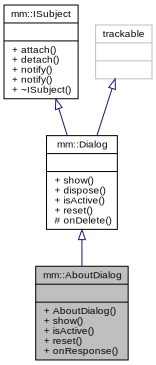
\includegraphics[width=228pt]{d1/dfc/classmm_1_1_about_dialog__inherit__graph}
\end{center}
\end{figure}


Diagramma di collaborazione per mm\+:\+:About\+Dialog\+:\nopagebreak
\begin{figure}[H]
\begin{center}
\leavevmode
\includegraphics[width=228pt]{da/dca/classmm_1_1_about_dialog__coll__graph}
\end{center}
\end{figure}
\subsection*{Membri pubblici}
\begin{DoxyCompactItemize}
\item 
\hyperlink{classmm_1_1_about_dialog_a489ffce563c6dae1dfef30518a778197}{About\+Dialog} ()
\item 
void \hyperlink{classmm_1_1_about_dialog_a9e06dc12f6950b74ccf6ccece693f108}{show} () override
\item 
bool \hyperlink{classmm_1_1_about_dialog_adc8aec0378d9d146c78eaf9a204dbf27}{is\+Active} () override
\item 
void \hyperlink{classmm_1_1_about_dialog_a21f5b0a7c9d8e43baab78e073d7ade2b}{reset} () override
\item 
void \hyperlink{classmm_1_1_about_dialog_a9a5feecb03e737d3bdbbf2a97dd7fbc4}{on\+Response} (int id)
\end{DoxyCompactItemize}


\subsection{Documentazione dei costruttori e dei distruttori}
\mbox{\Hypertarget{classmm_1_1_about_dialog_a489ffce563c6dae1dfef30518a778197}\label{classmm_1_1_about_dialog_a489ffce563c6dae1dfef30518a778197}} 
\index{mm\+::\+About\+Dialog@{mm\+::\+About\+Dialog}!About\+Dialog@{About\+Dialog}}
\index{About\+Dialog@{About\+Dialog}!mm\+::\+About\+Dialog@{mm\+::\+About\+Dialog}}
\subsubsection{\texorpdfstring{About\+Dialog()}{AboutDialog()}}
{\footnotesize\ttfamily mm\+::\+About\+Dialog\+::\+About\+Dialog (\begin{DoxyParamCaption}{ }\end{DoxyParamCaption})}



\subsection{Documentazione delle funzioni membro}
\mbox{\Hypertarget{classmm_1_1_about_dialog_adc8aec0378d9d146c78eaf9a204dbf27}\label{classmm_1_1_about_dialog_adc8aec0378d9d146c78eaf9a204dbf27}} 
\index{mm\+::\+About\+Dialog@{mm\+::\+About\+Dialog}!is\+Active@{is\+Active}}
\index{is\+Active@{is\+Active}!mm\+::\+About\+Dialog@{mm\+::\+About\+Dialog}}
\subsubsection{\texorpdfstring{is\+Active()}{isActive()}}
{\footnotesize\ttfamily bool mm\+::\+About\+Dialog\+::is\+Active (\begin{DoxyParamCaption}{ }\end{DoxyParamCaption})\hspace{0.3cm}{\ttfamily [override]}, {\ttfamily [virtual]}}



Implementa \hyperlink{classmm_1_1_dialog_a22abaf4e90b6fdca5c20039f6b9e15ac}{mm\+::\+Dialog}.

\mbox{\Hypertarget{classmm_1_1_about_dialog_a9a5feecb03e737d3bdbbf2a97dd7fbc4}\label{classmm_1_1_about_dialog_a9a5feecb03e737d3bdbbf2a97dd7fbc4}} 
\index{mm\+::\+About\+Dialog@{mm\+::\+About\+Dialog}!on\+Response@{on\+Response}}
\index{on\+Response@{on\+Response}!mm\+::\+About\+Dialog@{mm\+::\+About\+Dialog}}
\subsubsection{\texorpdfstring{on\+Response()}{onResponse()}}
{\footnotesize\ttfamily void mm\+::\+About\+Dialog\+::on\+Response (\begin{DoxyParamCaption}\item[{int}]{id }\end{DoxyParamCaption})}

\mbox{\Hypertarget{classmm_1_1_about_dialog_a21f5b0a7c9d8e43baab78e073d7ade2b}\label{classmm_1_1_about_dialog_a21f5b0a7c9d8e43baab78e073d7ade2b}} 
\index{mm\+::\+About\+Dialog@{mm\+::\+About\+Dialog}!reset@{reset}}
\index{reset@{reset}!mm\+::\+About\+Dialog@{mm\+::\+About\+Dialog}}
\subsubsection{\texorpdfstring{reset()}{reset()}}
{\footnotesize\ttfamily void mm\+::\+About\+Dialog\+::reset (\begin{DoxyParamCaption}{ }\end{DoxyParamCaption})\hspace{0.3cm}{\ttfamily [override]}, {\ttfamily [virtual]}}



Implementa \hyperlink{classmm_1_1_dialog_abe6e5ac072c12c06971f60491f079d80}{mm\+::\+Dialog}.

\mbox{\Hypertarget{classmm_1_1_about_dialog_a9e06dc12f6950b74ccf6ccece693f108}\label{classmm_1_1_about_dialog_a9e06dc12f6950b74ccf6ccece693f108}} 
\index{mm\+::\+About\+Dialog@{mm\+::\+About\+Dialog}!show@{show}}
\index{show@{show}!mm\+::\+About\+Dialog@{mm\+::\+About\+Dialog}}
\subsubsection{\texorpdfstring{show()}{show()}}
{\footnotesize\ttfamily void mm\+::\+About\+Dialog\+::show (\begin{DoxyParamCaption}{ }\end{DoxyParamCaption})\hspace{0.3cm}{\ttfamily [override]}, {\ttfamily [virtual]}}



Implementa \hyperlink{classmm_1_1_dialog_afda4b0dc7c0ac027c4b8fdb95713700f}{mm\+::\+Dialog}.



La documentazione per questa classe è stata generata a partire dai seguenti file\+:\begin{DoxyCompactItemize}
\item 
code/gui/\hyperlink{_about_dialog_8hpp}{About\+Dialog.\+hpp}\item 
code/gui/\hyperlink{_about_dialog_8cpp}{About\+Dialog.\+cpp}\end{DoxyCompactItemize}

\hypertarget{classmm_1_1_add_patient_dialog}{}\section{Riferimenti per la classe mm\+:\+:Add\+Patient\+Dialog}
\label{classmm_1_1_add_patient_dialog}\index{mm\+::\+Add\+Patient\+Dialog@{mm\+::\+Add\+Patient\+Dialog}}


{\ttfamily \#include $<$Add\+Patient\+Dialog.\+hpp$>$}



Diagramma delle classi per mm\+:\+:Add\+Patient\+Dialog\nopagebreak
\begin{figure}[H]
\begin{center}
\leavevmode
\includegraphics[width=228pt]{d7/d63/classmm_1_1_add_patient_dialog__inherit__graph}
\end{center}
\end{figure}


Diagramma di collaborazione per mm\+:\+:Add\+Patient\+Dialog\+:\nopagebreak
\begin{figure}[H]
\begin{center}
\leavevmode
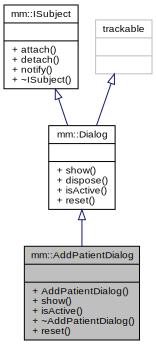
\includegraphics[width=228pt]{d5/d54/classmm_1_1_add_patient_dialog__coll__graph}
\end{center}
\end{figure}
\subsection*{Membri pubblici}
\begin{DoxyCompactItemize}
\item 
\hyperlink{classmm_1_1_add_patient_dialog_ad81abcf242a1c103f76c1fd4c6406b57}{Add\+Patient\+Dialog} ()
\item 
void \hyperlink{classmm_1_1_add_patient_dialog_a0247912794984eb19c43842ab9037708}{show} () override
\item 
bool \hyperlink{classmm_1_1_add_patient_dialog_a459a8acbec1c8a5a87e00f23402d3b5d}{is\+Active} () override
\item 
\hyperlink{classmm_1_1_add_patient_dialog_ab78d97d19d77fe6f47fbcd8af6a7b709}{$\sim$\+Add\+Patient\+Dialog} () override
\item 
void \hyperlink{classmm_1_1_add_patient_dialog_a64c8c2ea3b1c69a858f4eaec1854270a}{reset} () override
\end{DoxyCompactItemize}


\subsection{Documentazione dei costruttori e dei distruttori}
\mbox{\Hypertarget{classmm_1_1_add_patient_dialog_ad81abcf242a1c103f76c1fd4c6406b57}\label{classmm_1_1_add_patient_dialog_ad81abcf242a1c103f76c1fd4c6406b57}} 
\index{mm\+::\+Add\+Patient\+Dialog@{mm\+::\+Add\+Patient\+Dialog}!Add\+Patient\+Dialog@{Add\+Patient\+Dialog}}
\index{Add\+Patient\+Dialog@{Add\+Patient\+Dialog}!mm\+::\+Add\+Patient\+Dialog@{mm\+::\+Add\+Patient\+Dialog}}
\subsubsection{\texorpdfstring{Add\+Patient\+Dialog()}{AddPatientDialog()}}
{\footnotesize\ttfamily mm\+::\+Add\+Patient\+Dialog\+::\+Add\+Patient\+Dialog (\begin{DoxyParamCaption}{ }\end{DoxyParamCaption})}

\mbox{\Hypertarget{classmm_1_1_add_patient_dialog_ab78d97d19d77fe6f47fbcd8af6a7b709}\label{classmm_1_1_add_patient_dialog_ab78d97d19d77fe6f47fbcd8af6a7b709}} 
\index{mm\+::\+Add\+Patient\+Dialog@{mm\+::\+Add\+Patient\+Dialog}!````~Add\+Patient\+Dialog@{$\sim$\+Add\+Patient\+Dialog}}
\index{````~Add\+Patient\+Dialog@{$\sim$\+Add\+Patient\+Dialog}!mm\+::\+Add\+Patient\+Dialog@{mm\+::\+Add\+Patient\+Dialog}}
\subsubsection{\texorpdfstring{$\sim$\+Add\+Patient\+Dialog()}{~AddPatientDialog()}}
{\footnotesize\ttfamily mm\+::\+Add\+Patient\+Dialog\+::$\sim$\+Add\+Patient\+Dialog (\begin{DoxyParamCaption}{ }\end{DoxyParamCaption})\hspace{0.3cm}{\ttfamily [override]}}



\subsection{Documentazione delle funzioni membro}
\mbox{\Hypertarget{classmm_1_1_add_patient_dialog_a459a8acbec1c8a5a87e00f23402d3b5d}\label{classmm_1_1_add_patient_dialog_a459a8acbec1c8a5a87e00f23402d3b5d}} 
\index{mm\+::\+Add\+Patient\+Dialog@{mm\+::\+Add\+Patient\+Dialog}!is\+Active@{is\+Active}}
\index{is\+Active@{is\+Active}!mm\+::\+Add\+Patient\+Dialog@{mm\+::\+Add\+Patient\+Dialog}}
\subsubsection{\texorpdfstring{is\+Active()}{isActive()}}
{\footnotesize\ttfamily bool mm\+::\+Add\+Patient\+Dialog\+::is\+Active (\begin{DoxyParamCaption}{ }\end{DoxyParamCaption})\hspace{0.3cm}{\ttfamily [override]}, {\ttfamily [virtual]}}



Implementa \hyperlink{classmm_1_1_dialog_a22abaf4e90b6fdca5c20039f6b9e15ac}{mm\+::\+Dialog}.

\mbox{\Hypertarget{classmm_1_1_add_patient_dialog_a64c8c2ea3b1c69a858f4eaec1854270a}\label{classmm_1_1_add_patient_dialog_a64c8c2ea3b1c69a858f4eaec1854270a}} 
\index{mm\+::\+Add\+Patient\+Dialog@{mm\+::\+Add\+Patient\+Dialog}!reset@{reset}}
\index{reset@{reset}!mm\+::\+Add\+Patient\+Dialog@{mm\+::\+Add\+Patient\+Dialog}}
\subsubsection{\texorpdfstring{reset()}{reset()}}
{\footnotesize\ttfamily void mm\+::\+Add\+Patient\+Dialog\+::reset (\begin{DoxyParamCaption}{ }\end{DoxyParamCaption})\hspace{0.3cm}{\ttfamily [override]}, {\ttfamily [virtual]}}



Implementa \hyperlink{classmm_1_1_dialog_abe6e5ac072c12c06971f60491f079d80}{mm\+::\+Dialog}.

\mbox{\Hypertarget{classmm_1_1_add_patient_dialog_a0247912794984eb19c43842ab9037708}\label{classmm_1_1_add_patient_dialog_a0247912794984eb19c43842ab9037708}} 
\index{mm\+::\+Add\+Patient\+Dialog@{mm\+::\+Add\+Patient\+Dialog}!show@{show}}
\index{show@{show}!mm\+::\+Add\+Patient\+Dialog@{mm\+::\+Add\+Patient\+Dialog}}
\subsubsection{\texorpdfstring{show()}{show()}}
{\footnotesize\ttfamily void mm\+::\+Add\+Patient\+Dialog\+::show (\begin{DoxyParamCaption}{ }\end{DoxyParamCaption})\hspace{0.3cm}{\ttfamily [override]}, {\ttfamily [virtual]}}



Implementa \hyperlink{classmm_1_1_dialog_afda4b0dc7c0ac027c4b8fdb95713700f}{mm\+::\+Dialog}.



La documentazione per questa classe è stata generata a partire dai seguenti file\+:\begin{DoxyCompactItemize}
\item 
code/gui/\hyperlink{_add_patient_dialog_8hpp}{Add\+Patient\+Dialog.\+hpp}\item 
code/gui/\hyperlink{_add_patient_dialog_8cpp}{Add\+Patient\+Dialog.\+cpp}\end{DoxyCompactItemize}

\hypertarget{classmm_1_1_add_prescription_dialog}{}\section{Riferimenti per la classe mm\+:\+:Add\+Prescription\+Dialog}
\label{classmm_1_1_add_prescription_dialog}\index{mm\+::\+Add\+Prescription\+Dialog@{mm\+::\+Add\+Prescription\+Dialog}}


{\ttfamily \#include $<$Add\+Prescription\+Dialog.\+hpp$>$}



Diagramma delle classi per mm\+:\+:Add\+Prescription\+Dialog\nopagebreak
\begin{figure}[H]
\begin{center}
\leavevmode
\includegraphics[width=228pt]{d5/d29/classmm_1_1_add_prescription_dialog__inherit__graph}
\end{center}
\end{figure}


Diagramma di collaborazione per mm\+:\+:Add\+Prescription\+Dialog\+:\nopagebreak
\begin{figure}[H]
\begin{center}
\leavevmode
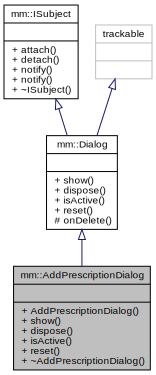
\includegraphics[width=228pt]{d6/dff/classmm_1_1_add_prescription_dialog__coll__graph}
\end{center}
\end{figure}
\subsection*{Membri pubblici}
\begin{DoxyCompactItemize}
\item 
\hyperlink{classmm_1_1_add_prescription_dialog_a0956469781e124fbfd283212bf1796ec}{Add\+Prescription\+Dialog} ()
\item 
void \hyperlink{classmm_1_1_add_prescription_dialog_aa1c86141b2d45e141684bd99d557b8e4}{show} () override
\item 
void \hyperlink{classmm_1_1_add_prescription_dialog_aacb58c7617be2323d91cd5ab2f28e354}{dispose} () override
\item 
bool \hyperlink{classmm_1_1_add_prescription_dialog_a4ff93500e8fd90512dc4575147b2c910}{is\+Active} () override
\item 
void \hyperlink{classmm_1_1_add_prescription_dialog_a6ace04587432a197436bb04c7b68d60d}{reset} () override
\end{DoxyCompactItemize}


\subsection{Documentazione dei costruttori e dei distruttori}
\mbox{\Hypertarget{classmm_1_1_add_prescription_dialog_a0956469781e124fbfd283212bf1796ec}\label{classmm_1_1_add_prescription_dialog_a0956469781e124fbfd283212bf1796ec}} 
\index{mm\+::\+Add\+Prescription\+Dialog@{mm\+::\+Add\+Prescription\+Dialog}!Add\+Prescription\+Dialog@{Add\+Prescription\+Dialog}}
\index{Add\+Prescription\+Dialog@{Add\+Prescription\+Dialog}!mm\+::\+Add\+Prescription\+Dialog@{mm\+::\+Add\+Prescription\+Dialog}}
\subsubsection{\texorpdfstring{Add\+Prescription\+Dialog()}{AddPrescriptionDialog()}}
{\footnotesize\ttfamily mm\+::\+Add\+Prescription\+Dialog\+::\+Add\+Prescription\+Dialog (\begin{DoxyParamCaption}{ }\end{DoxyParamCaption})}



\subsection{Documentazione delle funzioni membro}
\mbox{\Hypertarget{classmm_1_1_add_prescription_dialog_aacb58c7617be2323d91cd5ab2f28e354}\label{classmm_1_1_add_prescription_dialog_aacb58c7617be2323d91cd5ab2f28e354}} 
\index{mm\+::\+Add\+Prescription\+Dialog@{mm\+::\+Add\+Prescription\+Dialog}!dispose@{dispose}}
\index{dispose@{dispose}!mm\+::\+Add\+Prescription\+Dialog@{mm\+::\+Add\+Prescription\+Dialog}}
\subsubsection{\texorpdfstring{dispose()}{dispose()}}
{\footnotesize\ttfamily void mm\+::\+Add\+Prescription\+Dialog\+::dispose (\begin{DoxyParamCaption}{ }\end{DoxyParamCaption})\hspace{0.3cm}{\ttfamily [override]}, {\ttfamily [virtual]}}



Implementa \hyperlink{classmm_1_1_dialog_a3f2e361836af48ee3808f4dd6e4f8e48}{mm\+::\+Dialog}.

\mbox{\Hypertarget{classmm_1_1_add_prescription_dialog_a4ff93500e8fd90512dc4575147b2c910}\label{classmm_1_1_add_prescription_dialog_a4ff93500e8fd90512dc4575147b2c910}} 
\index{mm\+::\+Add\+Prescription\+Dialog@{mm\+::\+Add\+Prescription\+Dialog}!is\+Active@{is\+Active}}
\index{is\+Active@{is\+Active}!mm\+::\+Add\+Prescription\+Dialog@{mm\+::\+Add\+Prescription\+Dialog}}
\subsubsection{\texorpdfstring{is\+Active()}{isActive()}}
{\footnotesize\ttfamily bool mm\+::\+Add\+Prescription\+Dialog\+::is\+Active (\begin{DoxyParamCaption}{ }\end{DoxyParamCaption})\hspace{0.3cm}{\ttfamily [override]}, {\ttfamily [virtual]}}



Implementa \hyperlink{classmm_1_1_dialog_a22abaf4e90b6fdca5c20039f6b9e15ac}{mm\+::\+Dialog}.

\mbox{\Hypertarget{classmm_1_1_add_prescription_dialog_a6ace04587432a197436bb04c7b68d60d}\label{classmm_1_1_add_prescription_dialog_a6ace04587432a197436bb04c7b68d60d}} 
\index{mm\+::\+Add\+Prescription\+Dialog@{mm\+::\+Add\+Prescription\+Dialog}!reset@{reset}}
\index{reset@{reset}!mm\+::\+Add\+Prescription\+Dialog@{mm\+::\+Add\+Prescription\+Dialog}}
\subsubsection{\texorpdfstring{reset()}{reset()}}
{\footnotesize\ttfamily void mm\+::\+Add\+Prescription\+Dialog\+::reset (\begin{DoxyParamCaption}{ }\end{DoxyParamCaption})\hspace{0.3cm}{\ttfamily [override]}, {\ttfamily [virtual]}}



Implementa \hyperlink{classmm_1_1_dialog_abe6e5ac072c12c06971f60491f079d80}{mm\+::\+Dialog}.

\mbox{\Hypertarget{classmm_1_1_add_prescription_dialog_aa1c86141b2d45e141684bd99d557b8e4}\label{classmm_1_1_add_prescription_dialog_aa1c86141b2d45e141684bd99d557b8e4}} 
\index{mm\+::\+Add\+Prescription\+Dialog@{mm\+::\+Add\+Prescription\+Dialog}!show@{show}}
\index{show@{show}!mm\+::\+Add\+Prescription\+Dialog@{mm\+::\+Add\+Prescription\+Dialog}}
\subsubsection{\texorpdfstring{show()}{show()}}
{\footnotesize\ttfamily void mm\+::\+Add\+Prescription\+Dialog\+::show (\begin{DoxyParamCaption}{ }\end{DoxyParamCaption})\hspace{0.3cm}{\ttfamily [override]}, {\ttfamily [virtual]}}



Implementa \hyperlink{classmm_1_1_dialog_afda4b0dc7c0ac027c4b8fdb95713700f}{mm\+::\+Dialog}.



La documentazione per questa classe è stata generata a partire dai seguenti file\+:\begin{DoxyCompactItemize}
\item 
code/gui/\hyperlink{_add_prescription_dialog_8hpp}{Add\+Prescription\+Dialog.\+hpp}\item 
code/gui/\hyperlink{_add_prescription_dialog_8cpp}{Add\+Prescription\+Dialog.\+cpp}\end{DoxyCompactItemize}

\hypertarget{classmm_1_1_configuration}{}\section{Riferimenti per la classe mm\+:\+:Configuration}
\label{classmm_1_1_configuration}\index{mm\+::\+Configuration@{mm\+::\+Configuration}}


Singleton che mantiene le configurazioni dell\textquotesingle{}intera applicazione.  




{\ttfamily \#include $<$Configuration.\+hpp$>$}



Diagramma di collaborazione per mm\+:\+:Configuration\+:\nopagebreak
\begin{figure}[H]
\begin{center}
\leavevmode
\includegraphics[width=206pt]{dc/d7c/classmm_1_1_configuration__coll__graph}
\end{center}
\end{figure}
\subsection*{Membri pubblici}
\begin{DoxyCompactItemize}
\item 
\hyperlink{classmm_1_1_configuration_a71e5c0e1ad7d82d6a14895a4e85d83b7}{Configuration} (const \hyperlink{classmm_1_1_configuration}{Configuration} \&old)=delete
\item 
const \hyperlink{classmm_1_1_configuration}{Configuration} \& \hyperlink{classmm_1_1_configuration_a3077aebf459758dce4be716a8ddcb090}{operator=} (const \hyperlink{classmm_1_1_configuration}{Configuration} \&old)=delete
\item 
{\footnotesize template$<$typename T $>$ }\\T \hyperlink{classmm_1_1_configuration_a30374c407050b9fb3f05dd3c2c01202d}{get} (const std\+::string \&key) const noexcept(false)
\begin{DoxyCompactList}\small\item\em Cerca nel file json la chiave {\ttfamily key}, se questa non viene trovata lancia l\textquotesingle{}apposita eccezione altrimenti ritorna l\textquotesingle{}oggetto corrispondente a {\ttfamily key} nel file. \end{DoxyCompactList}\end{DoxyCompactItemize}
\subsection*{Membri pubblici statici}
\begin{DoxyCompactItemize}
\item 
static \hyperlink{classmm_1_1_configuration}{Configuration} \& \hyperlink{classmm_1_1_configuration_a5cfc5ea56062f53ef9fbd274f6dbe79e}{get\+\_\+instance} () noexcept(false)
\begin{DoxyCompactList}\small\item\em Ritorna una reference ad un\textquotesingle{}istanza di tipo {\ttfamily \hyperlink{classmm_1_1_configuration}{Configuration}}. \end{DoxyCompactList}\item 
static const std\+::string \& \hyperlink{classmm_1_1_configuration_a631c8525beb91fb55d72eb6b58d2d68f}{get\+\_\+config\+\_\+file\+\_\+name} ()
\begin{DoxyCompactList}\small\item\em Ritorna una stringa contente il path dove viene cercato cercato il file json. \end{DoxyCompactList}\item 
static void \hyperlink{classmm_1_1_configuration_ad526b28d1a7f8c6f854352b840d2d7b4}{set\+\_\+config\+\_\+file\+\_\+name} (const std\+::string \&config\+\_\+file\+\_\+name)
\begin{DoxyCompactList}\small\item\em Serve per impostare il path dove trovare il file di configurazione. \end{DoxyCompactList}\end{DoxyCompactItemize}


\subsection{Descrizione dettagliata}
Singleton che mantiene le configurazioni dell\textquotesingle{}intera applicazione. 

I parametri di configurazione dell\textquotesingle{}applicazione devono essere salvati in un file in formato json. La classe si occupa sia di leggere che di fornire un\textquotesingle{}interfaccia semplice per ottenere un parametro dal file 

\subsection{Documentazione dei costruttori e dei distruttori}
\mbox{\Hypertarget{classmm_1_1_configuration_a71e5c0e1ad7d82d6a14895a4e85d83b7}\label{classmm_1_1_configuration_a71e5c0e1ad7d82d6a14895a4e85d83b7}} 
\index{mm\+::\+Configuration@{mm\+::\+Configuration}!Configuration@{Configuration}}
\index{Configuration@{Configuration}!mm\+::\+Configuration@{mm\+::\+Configuration}}
\subsubsection{\texorpdfstring{Configuration()}{Configuration()}}
{\footnotesize\ttfamily mm\+::\+Configuration\+::\+Configuration (\begin{DoxyParamCaption}\item[{const \hyperlink{classmm_1_1_configuration}{Configuration} \&}]{old }\end{DoxyParamCaption})\hspace{0.3cm}{\ttfamily [delete]}}



\subsection{Documentazione delle funzioni membro}
\mbox{\Hypertarget{classmm_1_1_configuration_a30374c407050b9fb3f05dd3c2c01202d}\label{classmm_1_1_configuration_a30374c407050b9fb3f05dd3c2c01202d}} 
\index{mm\+::\+Configuration@{mm\+::\+Configuration}!get@{get}}
\index{get@{get}!mm\+::\+Configuration@{mm\+::\+Configuration}}
\subsubsection{\texorpdfstring{get()}{get()}}
{\footnotesize\ttfamily template$<$typename T $>$ \\
T mm\+::\+Configuration\+::get (\begin{DoxyParamCaption}\item[{const std\+::string \&}]{key }\end{DoxyParamCaption}) const\hspace{0.3cm}{\ttfamily [inline]}, {\ttfamily [noexcept]}}



Cerca nel file json la chiave {\ttfamily key}, se questa non viene trovata lancia l\textquotesingle{}apposita eccezione altrimenti ritorna l\textquotesingle{}oggetto corrispondente a {\ttfamily key} nel file. 

N.\+B. {\ttfamily T} deve essere corrispondente al tipo di dato nel json, altrimenti sarà lanciata un eccezione.


\begin{DoxyTemplParams}{Template Parameters}
{\em T} & Tipo del dato di configurazione \\
\hline
\end{DoxyTemplParams}

\begin{DoxyParams}{Parametri}
{\em key} & Chiave da cercare nel file \\
\hline
\end{DoxyParams}
\begin{DoxyReturn}{Restituisce}
Oggetto di tipo {\ttfamily T} contenente i dati presenti nel file json alla chiave {\ttfamily key} 
\end{DoxyReturn}
\mbox{\Hypertarget{classmm_1_1_configuration_a631c8525beb91fb55d72eb6b58d2d68f}\label{classmm_1_1_configuration_a631c8525beb91fb55d72eb6b58d2d68f}} 
\index{mm\+::\+Configuration@{mm\+::\+Configuration}!get\+\_\+config\+\_\+file\+\_\+name@{get\+\_\+config\+\_\+file\+\_\+name}}
\index{get\+\_\+config\+\_\+file\+\_\+name@{get\+\_\+config\+\_\+file\+\_\+name}!mm\+::\+Configuration@{mm\+::\+Configuration}}
\subsubsection{\texorpdfstring{get\+\_\+config\+\_\+file\+\_\+name()}{get\_config\_file\_name()}}
{\footnotesize\ttfamily const std\+::string \& mm\+::\+Configuration\+::get\+\_\+config\+\_\+file\+\_\+name (\begin{DoxyParamCaption}{ }\end{DoxyParamCaption})\hspace{0.3cm}{\ttfamily [static]}}



Ritorna una stringa contente il path dove viene cercato cercato il file json. 

\begin{DoxyReturn}{Restituisce}
Il path del file di configurazione 
\end{DoxyReturn}
\mbox{\Hypertarget{classmm_1_1_configuration_a5cfc5ea56062f53ef9fbd274f6dbe79e}\label{classmm_1_1_configuration_a5cfc5ea56062f53ef9fbd274f6dbe79e}} 
\index{mm\+::\+Configuration@{mm\+::\+Configuration}!get\+\_\+instance@{get\+\_\+instance}}
\index{get\+\_\+instance@{get\+\_\+instance}!mm\+::\+Configuration@{mm\+::\+Configuration}}
\subsubsection{\texorpdfstring{get\+\_\+instance()}{get\_instance()}}
{\footnotesize\ttfamily \hyperlink{classmm_1_1_configuration}{mm\+::\+Configuration} \& mm\+::\+Configuration\+::get\+\_\+instance (\begin{DoxyParamCaption}{ }\end{DoxyParamCaption})\hspace{0.3cm}{\ttfamily [static]}, {\ttfamily [noexcept]}}



Ritorna una reference ad un\textquotesingle{}istanza di tipo {\ttfamily \hyperlink{classmm_1_1_configuration}{Configuration}}. 

Questa funzione non deve mai essere chiamata se prima non è stato chiamato (almeno una volta) il metodo \hyperlink{classmm_1_1_configuration_ad526b28d1a7f8c6f854352b840d2d7b4}{Configuration\+::set\+\_\+config\+\_\+file\+\_\+name()}.

N.\+B. Essendo il distruttore privato non è possibile cancellare l\textquotesingle{}oggetto al di fuori di questa classe

\begin{DoxyReturn}{Restituisce}
Istanza di \hyperlink{classmm_1_1_configuration}{Configuration} 
\end{DoxyReturn}
\mbox{\Hypertarget{classmm_1_1_configuration_a3077aebf459758dce4be716a8ddcb090}\label{classmm_1_1_configuration_a3077aebf459758dce4be716a8ddcb090}} 
\index{mm\+::\+Configuration@{mm\+::\+Configuration}!operator=@{operator=}}
\index{operator=@{operator=}!mm\+::\+Configuration@{mm\+::\+Configuration}}
\subsubsection{\texorpdfstring{operator=()}{operator=()}}
{\footnotesize\ttfamily const \hyperlink{classmm_1_1_configuration}{Configuration}\& mm\+::\+Configuration\+::operator= (\begin{DoxyParamCaption}\item[{const \hyperlink{classmm_1_1_configuration}{Configuration} \&}]{old }\end{DoxyParamCaption})\hspace{0.3cm}{\ttfamily [delete]}}

\mbox{\Hypertarget{classmm_1_1_configuration_ad526b28d1a7f8c6f854352b840d2d7b4}\label{classmm_1_1_configuration_ad526b28d1a7f8c6f854352b840d2d7b4}} 
\index{mm\+::\+Configuration@{mm\+::\+Configuration}!set\+\_\+config\+\_\+file\+\_\+name@{set\+\_\+config\+\_\+file\+\_\+name}}
\index{set\+\_\+config\+\_\+file\+\_\+name@{set\+\_\+config\+\_\+file\+\_\+name}!mm\+::\+Configuration@{mm\+::\+Configuration}}
\subsubsection{\texorpdfstring{set\+\_\+config\+\_\+file\+\_\+name()}{set\_config\_file\_name()}}
{\footnotesize\ttfamily void mm\+::\+Configuration\+::set\+\_\+config\+\_\+file\+\_\+name (\begin{DoxyParamCaption}\item[{const std\+::string \&}]{config\+\_\+file\+\_\+name }\end{DoxyParamCaption})\hspace{0.3cm}{\ttfamily [static]}}



Serve per impostare il path dove trovare il file di configurazione. 

N.\+B. Questa funzione {\bfseries deve} sempre essere chiamata prima di una qualsiasi chiamata a \hyperlink{classmm_1_1_configuration_a5cfc5ea56062f53ef9fbd274f6dbe79e}{Configuration\+::get\+\_\+instance}


\begin{DoxyParams}[1]{Parametri}
\mbox{\tt in}  & {\em config\+\_\+file\+\_\+name} & Una stringa contenente il path dove trovare il file \\
\hline
\end{DoxyParams}


La documentazione per questa classe è stata generata a partire dai seguenti file\+:\begin{DoxyCompactItemize}
\item 
code/\hyperlink{_configuration_8hpp}{Configuration.\+hpp}\item 
code/\hyperlink{_configuration_8cpp}{Configuration.\+cpp}\end{DoxyCompactItemize}

\hypertarget{structmm_1_1util_1_1_date}{}\section{Riferimenti per la struct mm\+:\+:util\+:\+:Date}
\label{structmm_1_1util_1_1_date}\index{mm\+::util\+::\+Date@{mm\+::util\+::\+Date}}


{\ttfamily \#include $<$Date.\+hpp$>$}



Diagramma di collaborazione per mm\+:\+:util\+:\+:Date\+:
\nopagebreak
\begin{figure}[H]
\begin{center}
\leavevmode
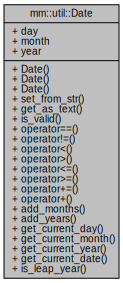
\includegraphics[width=195pt]{d4/d70/structmm_1_1util_1_1_date__coll__graph}
\end{center}
\end{figure}
\subsection*{Membri pubblici}
\begin{DoxyCompactItemize}
\item 
\mbox{\hyperlink{structmm_1_1util_1_1_date_afe2513fbf246f7f3e61e7d1a06d0e6d0}{Date}} (int \mbox{\hyperlink{structmm_1_1util_1_1_date_a6a697c80be4f09cdb4ee400721314d87}{day}}, int \mbox{\hyperlink{structmm_1_1util_1_1_date_a018f3e7261b88c9a47aae5b08120b331}{month}}, int \mbox{\hyperlink{structmm_1_1util_1_1_date_a318909ff98468f29c7912fa9cffea079}{year}})
\item 
\mbox{\hyperlink{structmm_1_1util_1_1_date_a9aaf2c2d5171e081541831c4a756232e}{Date}} ()
\item 
\mbox{\hyperlink{structmm_1_1util_1_1_date_a9065cbdea26e95cfbb6537a5ba06f45d}{Date}} (const std\+::string \&str)
\item 
void \mbox{\hyperlink{structmm_1_1util_1_1_date_a9140b9c53f02f7385af15684c81c5ed0}{set\+\_\+from\+\_\+str}} (std\+::string str)
\item 
const std\+::string \mbox{\hyperlink{structmm_1_1util_1_1_date_aa32e7e2771581a860a49a59cdbcec8f8}{get\+\_\+as\+\_\+text}} ()
\item 
bool \mbox{\hyperlink{structmm_1_1util_1_1_date_ae4b2c74f7e6ebfed3daaafc999af31ba}{is\+\_\+valid}} ()
\item 
bool \mbox{\hyperlink{structmm_1_1util_1_1_date_a55071cbbf31cd8956cd4a7d5116e0d95}{operator==}} (const \mbox{\hyperlink{structmm_1_1util_1_1_date}{Date}} \&rhs) const
\item 
bool \mbox{\hyperlink{structmm_1_1util_1_1_date_a9f2556bcc1150f5542d59b2f9078ee1b}{operator!=}} (const \mbox{\hyperlink{structmm_1_1util_1_1_date}{Date}} \&rhs) const
\item 
bool \mbox{\hyperlink{structmm_1_1util_1_1_date_acb395628bc3074f0f5f782e39f7ecbbf}{operator$<$}} (const \mbox{\hyperlink{structmm_1_1util_1_1_date}{Date}} \&rhs) const
\item 
bool \mbox{\hyperlink{structmm_1_1util_1_1_date_a5b070fd2cd4a72cf74849abd9244b6d3}{operator$>$}} (const \mbox{\hyperlink{structmm_1_1util_1_1_date}{Date}} \&rhs) const
\item 
bool \mbox{\hyperlink{structmm_1_1util_1_1_date_aec9077b20de935d88cc03e4c454915a3}{operator$<$=}} (const \mbox{\hyperlink{structmm_1_1util_1_1_date}{Date}} \&rhs) const
\item 
bool \mbox{\hyperlink{structmm_1_1util_1_1_date_ab0dc9872f7646c748d492afcff696a0d}{operator$>$=}} (const \mbox{\hyperlink{structmm_1_1util_1_1_date}{Date}} \&rhs) const
\item 
void \mbox{\hyperlink{structmm_1_1util_1_1_date_a9aecce8821f2448c0d2d36a5fbf455b1}{operator+=}} (int days)
\item 
\mbox{\hyperlink{structmm_1_1util_1_1_date}{Date}} \mbox{\hyperlink{structmm_1_1util_1_1_date_a36a932c021e6e5e9ebed44752b78fd7c}{operator+}} (int days)
\item 
void \mbox{\hyperlink{structmm_1_1util_1_1_date_ae875de5d40ab9dfa1f1e22cb8a847b60}{add\+\_\+months}} (unsigned int months)
\item 
void \mbox{\hyperlink{structmm_1_1util_1_1_date_a5ca08a73148a58f47847a30040eee70b}{add\+\_\+years}} (unsigned int years)
\end{DoxyCompactItemize}
\subsection*{Membri pubblici statici}
\begin{DoxyCompactItemize}
\item 
static int \mbox{\hyperlink{structmm_1_1util_1_1_date_ad5ed2bc80bbaa949aa13707a73064345}{get\+\_\+current\+\_\+day}} ()
\item 
static int \mbox{\hyperlink{structmm_1_1util_1_1_date_ab3da347f3603aa3a7fe057a5a0d012d2}{get\+\_\+current\+\_\+month}} ()
\item 
static int \mbox{\hyperlink{structmm_1_1util_1_1_date_afec17843da4296a2341290107901eaa5}{get\+\_\+current\+\_\+year}} ()
\item 
static \mbox{\hyperlink{structmm_1_1util_1_1_date}{Date}} \mbox{\hyperlink{structmm_1_1util_1_1_date_af0758fad7ef32fd535db3295136466eb}{get\+\_\+current\+\_\+date}} ()
\item 
static bool \mbox{\hyperlink{structmm_1_1util_1_1_date_a89c7d3f4d8af79878a28815ffbe2e536}{is\+\_\+leap\+\_\+year}} (int \mbox{\hyperlink{structmm_1_1util_1_1_date_a318909ff98468f29c7912fa9cffea079}{year}})
\end{DoxyCompactItemize}
\subsection*{Attributi pubblici}
\begin{DoxyCompactItemize}
\item 
int \mbox{\hyperlink{structmm_1_1util_1_1_date_a6a697c80be4f09cdb4ee400721314d87}{day}}
\item 
int \mbox{\hyperlink{structmm_1_1util_1_1_date_a018f3e7261b88c9a47aae5b08120b331}{month}}
\item 
int \mbox{\hyperlink{structmm_1_1util_1_1_date_a318909ff98468f29c7912fa9cffea079}{year}}
\end{DoxyCompactItemize}
\subsection*{Friend}
\begin{DoxyCompactItemize}
\item 
std\+::ostream \& \mbox{\hyperlink{structmm_1_1util_1_1_date_a1862604492a841a6b98e1a3061d95b96}{operator$<$$<$}} (std\+::ostream \&os, const \mbox{\hyperlink{structmm_1_1util_1_1_date}{Date}} \&date)
\end{DoxyCompactItemize}


\subsection{Documentazione dei costruttori e dei distruttori}
\mbox{\Hypertarget{structmm_1_1util_1_1_date_afe2513fbf246f7f3e61e7d1a06d0e6d0}\label{structmm_1_1util_1_1_date_afe2513fbf246f7f3e61e7d1a06d0e6d0}} 
\index{mm\+::util\+::\+Date@{mm\+::util\+::\+Date}!Date@{Date}}
\index{Date@{Date}!mm\+::util\+::\+Date@{mm\+::util\+::\+Date}}
\subsubsection{\texorpdfstring{Date()}{Date()}\hspace{0.1cm}{\footnotesize\ttfamily [1/3]}}
{\footnotesize\ttfamily mm\+::util\+::\+Date\+::\+Date (\begin{DoxyParamCaption}\item[{int}]{day,  }\item[{int}]{month,  }\item[{int}]{year }\end{DoxyParamCaption})}

Project Elaborato\+\_\+\+I\+N\+G\+\_\+\+SW \begin{DoxyAuthor}{Autore}
Noè Murr, Mirko Morati \mbox{\hyperlink{structmm_1_1util_1_1_date}{Date}} implementation 
\end{DoxyAuthor}
\mbox{\Hypertarget{structmm_1_1util_1_1_date_a9aaf2c2d5171e081541831c4a756232e}\label{structmm_1_1util_1_1_date_a9aaf2c2d5171e081541831c4a756232e}} 
\index{mm\+::util\+::\+Date@{mm\+::util\+::\+Date}!Date@{Date}}
\index{Date@{Date}!mm\+::util\+::\+Date@{mm\+::util\+::\+Date}}
\subsubsection{\texorpdfstring{Date()}{Date()}\hspace{0.1cm}{\footnotesize\ttfamily [2/3]}}
{\footnotesize\ttfamily mm\+::util\+::\+Date\+::\+Date (\begin{DoxyParamCaption}{ }\end{DoxyParamCaption})}

\mbox{\Hypertarget{structmm_1_1util_1_1_date_a9065cbdea26e95cfbb6537a5ba06f45d}\label{structmm_1_1util_1_1_date_a9065cbdea26e95cfbb6537a5ba06f45d}} 
\index{mm\+::util\+::\+Date@{mm\+::util\+::\+Date}!Date@{Date}}
\index{Date@{Date}!mm\+::util\+::\+Date@{mm\+::util\+::\+Date}}
\subsubsection{\texorpdfstring{Date()}{Date()}\hspace{0.1cm}{\footnotesize\ttfamily [3/3]}}
{\footnotesize\ttfamily mm\+::util\+::\+Date\+::\+Date (\begin{DoxyParamCaption}\item[{const std\+::string \&}]{str }\end{DoxyParamCaption})}



\subsection{Documentazione delle funzioni membro}
\mbox{\Hypertarget{structmm_1_1util_1_1_date_ae875de5d40ab9dfa1f1e22cb8a847b60}\label{structmm_1_1util_1_1_date_ae875de5d40ab9dfa1f1e22cb8a847b60}} 
\index{mm\+::util\+::\+Date@{mm\+::util\+::\+Date}!add\+\_\+months@{add\+\_\+months}}
\index{add\+\_\+months@{add\+\_\+months}!mm\+::util\+::\+Date@{mm\+::util\+::\+Date}}
\subsubsection{\texorpdfstring{add\+\_\+months()}{add\_months()}}
{\footnotesize\ttfamily void mm\+::util\+::\+Date\+::add\+\_\+months (\begin{DoxyParamCaption}\item[{unsigned int}]{months }\end{DoxyParamCaption})}

\mbox{\Hypertarget{structmm_1_1util_1_1_date_a5ca08a73148a58f47847a30040eee70b}\label{structmm_1_1util_1_1_date_a5ca08a73148a58f47847a30040eee70b}} 
\index{mm\+::util\+::\+Date@{mm\+::util\+::\+Date}!add\+\_\+years@{add\+\_\+years}}
\index{add\+\_\+years@{add\+\_\+years}!mm\+::util\+::\+Date@{mm\+::util\+::\+Date}}
\subsubsection{\texorpdfstring{add\+\_\+years()}{add\_years()}}
{\footnotesize\ttfamily void mm\+::util\+::\+Date\+::add\+\_\+years (\begin{DoxyParamCaption}\item[{unsigned int}]{years }\end{DoxyParamCaption})}

\mbox{\Hypertarget{structmm_1_1util_1_1_date_aa32e7e2771581a860a49a59cdbcec8f8}\label{structmm_1_1util_1_1_date_aa32e7e2771581a860a49a59cdbcec8f8}} 
\index{mm\+::util\+::\+Date@{mm\+::util\+::\+Date}!get\+\_\+as\+\_\+text@{get\+\_\+as\+\_\+text}}
\index{get\+\_\+as\+\_\+text@{get\+\_\+as\+\_\+text}!mm\+::util\+::\+Date@{mm\+::util\+::\+Date}}
\subsubsection{\texorpdfstring{get\+\_\+as\+\_\+text()}{get\_as\_text()}}
{\footnotesize\ttfamily const std\+::string mm\+::util\+::\+Date\+::get\+\_\+as\+\_\+text (\begin{DoxyParamCaption}{ }\end{DoxyParamCaption})}

\mbox{\Hypertarget{structmm_1_1util_1_1_date_af0758fad7ef32fd535db3295136466eb}\label{structmm_1_1util_1_1_date_af0758fad7ef32fd535db3295136466eb}} 
\index{mm\+::util\+::\+Date@{mm\+::util\+::\+Date}!get\+\_\+current\+\_\+date@{get\+\_\+current\+\_\+date}}
\index{get\+\_\+current\+\_\+date@{get\+\_\+current\+\_\+date}!mm\+::util\+::\+Date@{mm\+::util\+::\+Date}}
\subsubsection{\texorpdfstring{get\+\_\+current\+\_\+date()}{get\_current\_date()}}
{\footnotesize\ttfamily \mbox{\hyperlink{structmm_1_1util_1_1_date}{mm\+::util\+::\+Date}} mm\+::util\+::\+Date\+::get\+\_\+current\+\_\+date (\begin{DoxyParamCaption}{ }\end{DoxyParamCaption})\hspace{0.3cm}{\ttfamily [static]}}

\mbox{\Hypertarget{structmm_1_1util_1_1_date_ad5ed2bc80bbaa949aa13707a73064345}\label{structmm_1_1util_1_1_date_ad5ed2bc80bbaa949aa13707a73064345}} 
\index{mm\+::util\+::\+Date@{mm\+::util\+::\+Date}!get\+\_\+current\+\_\+day@{get\+\_\+current\+\_\+day}}
\index{get\+\_\+current\+\_\+day@{get\+\_\+current\+\_\+day}!mm\+::util\+::\+Date@{mm\+::util\+::\+Date}}
\subsubsection{\texorpdfstring{get\+\_\+current\+\_\+day()}{get\_current\_day()}}
{\footnotesize\ttfamily int mm\+::util\+::\+Date\+::get\+\_\+current\+\_\+day (\begin{DoxyParamCaption}{ }\end{DoxyParamCaption})\hspace{0.3cm}{\ttfamily [static]}}

\mbox{\Hypertarget{structmm_1_1util_1_1_date_ab3da347f3603aa3a7fe057a5a0d012d2}\label{structmm_1_1util_1_1_date_ab3da347f3603aa3a7fe057a5a0d012d2}} 
\index{mm\+::util\+::\+Date@{mm\+::util\+::\+Date}!get\+\_\+current\+\_\+month@{get\+\_\+current\+\_\+month}}
\index{get\+\_\+current\+\_\+month@{get\+\_\+current\+\_\+month}!mm\+::util\+::\+Date@{mm\+::util\+::\+Date}}
\subsubsection{\texorpdfstring{get\+\_\+current\+\_\+month()}{get\_current\_month()}}
{\footnotesize\ttfamily int mm\+::util\+::\+Date\+::get\+\_\+current\+\_\+month (\begin{DoxyParamCaption}{ }\end{DoxyParamCaption})\hspace{0.3cm}{\ttfamily [static]}}

\mbox{\Hypertarget{structmm_1_1util_1_1_date_afec17843da4296a2341290107901eaa5}\label{structmm_1_1util_1_1_date_afec17843da4296a2341290107901eaa5}} 
\index{mm\+::util\+::\+Date@{mm\+::util\+::\+Date}!get\+\_\+current\+\_\+year@{get\+\_\+current\+\_\+year}}
\index{get\+\_\+current\+\_\+year@{get\+\_\+current\+\_\+year}!mm\+::util\+::\+Date@{mm\+::util\+::\+Date}}
\subsubsection{\texorpdfstring{get\+\_\+current\+\_\+year()}{get\_current\_year()}}
{\footnotesize\ttfamily int mm\+::util\+::\+Date\+::get\+\_\+current\+\_\+year (\begin{DoxyParamCaption}{ }\end{DoxyParamCaption})\hspace{0.3cm}{\ttfamily [static]}}

\mbox{\Hypertarget{structmm_1_1util_1_1_date_a89c7d3f4d8af79878a28815ffbe2e536}\label{structmm_1_1util_1_1_date_a89c7d3f4d8af79878a28815ffbe2e536}} 
\index{mm\+::util\+::\+Date@{mm\+::util\+::\+Date}!is\+\_\+leap\+\_\+year@{is\+\_\+leap\+\_\+year}}
\index{is\+\_\+leap\+\_\+year@{is\+\_\+leap\+\_\+year}!mm\+::util\+::\+Date@{mm\+::util\+::\+Date}}
\subsubsection{\texorpdfstring{is\+\_\+leap\+\_\+year()}{is\_leap\_year()}}
{\footnotesize\ttfamily static bool mm\+::util\+::\+Date\+::is\+\_\+leap\+\_\+year (\begin{DoxyParamCaption}\item[{int}]{year }\end{DoxyParamCaption})\hspace{0.3cm}{\ttfamily [inline]}, {\ttfamily [static]}}

\mbox{\Hypertarget{structmm_1_1util_1_1_date_ae4b2c74f7e6ebfed3daaafc999af31ba}\label{structmm_1_1util_1_1_date_ae4b2c74f7e6ebfed3daaafc999af31ba}} 
\index{mm\+::util\+::\+Date@{mm\+::util\+::\+Date}!is\+\_\+valid@{is\+\_\+valid}}
\index{is\+\_\+valid@{is\+\_\+valid}!mm\+::util\+::\+Date@{mm\+::util\+::\+Date}}
\subsubsection{\texorpdfstring{is\+\_\+valid()}{is\_valid()}}
{\footnotesize\ttfamily bool mm\+::util\+::\+Date\+::is\+\_\+valid (\begin{DoxyParamCaption}{ }\end{DoxyParamCaption})}

\mbox{\Hypertarget{structmm_1_1util_1_1_date_a9f2556bcc1150f5542d59b2f9078ee1b}\label{structmm_1_1util_1_1_date_a9f2556bcc1150f5542d59b2f9078ee1b}} 
\index{mm\+::util\+::\+Date@{mm\+::util\+::\+Date}!operator"!=@{operator"!=}}
\index{operator"!=@{operator"!=}!mm\+::util\+::\+Date@{mm\+::util\+::\+Date}}
\subsubsection{\texorpdfstring{operator"!=()}{operator!=()}}
{\footnotesize\ttfamily bool mm\+::util\+::\+Date\+::operator!= (\begin{DoxyParamCaption}\item[{const \mbox{\hyperlink{structmm_1_1util_1_1_date}{Date}} \&}]{rhs }\end{DoxyParamCaption}) const}

\mbox{\Hypertarget{structmm_1_1util_1_1_date_a36a932c021e6e5e9ebed44752b78fd7c}\label{structmm_1_1util_1_1_date_a36a932c021e6e5e9ebed44752b78fd7c}} 
\index{mm\+::util\+::\+Date@{mm\+::util\+::\+Date}!operator+@{operator+}}
\index{operator+@{operator+}!mm\+::util\+::\+Date@{mm\+::util\+::\+Date}}
\subsubsection{\texorpdfstring{operator+()}{operator+()}}
{\footnotesize\ttfamily \mbox{\hyperlink{structmm_1_1util_1_1_date}{mm\+::util\+::\+Date}} mm\+::util\+::\+Date\+::operator+ (\begin{DoxyParamCaption}\item[{int}]{days }\end{DoxyParamCaption})}

\mbox{\Hypertarget{structmm_1_1util_1_1_date_a9aecce8821f2448c0d2d36a5fbf455b1}\label{structmm_1_1util_1_1_date_a9aecce8821f2448c0d2d36a5fbf455b1}} 
\index{mm\+::util\+::\+Date@{mm\+::util\+::\+Date}!operator+=@{operator+=}}
\index{operator+=@{operator+=}!mm\+::util\+::\+Date@{mm\+::util\+::\+Date}}
\subsubsection{\texorpdfstring{operator+=()}{operator+=()}}
{\footnotesize\ttfamily void mm\+::util\+::\+Date\+::operator+= (\begin{DoxyParamCaption}\item[{int}]{days }\end{DoxyParamCaption})}

\mbox{\Hypertarget{structmm_1_1util_1_1_date_acb395628bc3074f0f5f782e39f7ecbbf}\label{structmm_1_1util_1_1_date_acb395628bc3074f0f5f782e39f7ecbbf}} 
\index{mm\+::util\+::\+Date@{mm\+::util\+::\+Date}!operator$<$@{operator$<$}}
\index{operator$<$@{operator$<$}!mm\+::util\+::\+Date@{mm\+::util\+::\+Date}}
\subsubsection{\texorpdfstring{operator$<$()}{operator<()}}
{\footnotesize\ttfamily bool mm\+::util\+::\+Date\+::operator$<$ (\begin{DoxyParamCaption}\item[{const \mbox{\hyperlink{structmm_1_1util_1_1_date}{Date}} \&}]{rhs }\end{DoxyParamCaption}) const}

\mbox{\Hypertarget{structmm_1_1util_1_1_date_aec9077b20de935d88cc03e4c454915a3}\label{structmm_1_1util_1_1_date_aec9077b20de935d88cc03e4c454915a3}} 
\index{mm\+::util\+::\+Date@{mm\+::util\+::\+Date}!operator$<$=@{operator$<$=}}
\index{operator$<$=@{operator$<$=}!mm\+::util\+::\+Date@{mm\+::util\+::\+Date}}
\subsubsection{\texorpdfstring{operator$<$=()}{operator<=()}}
{\footnotesize\ttfamily bool mm\+::util\+::\+Date\+::operator$<$= (\begin{DoxyParamCaption}\item[{const \mbox{\hyperlink{structmm_1_1util_1_1_date}{Date}} \&}]{rhs }\end{DoxyParamCaption}) const}

\mbox{\Hypertarget{structmm_1_1util_1_1_date_a55071cbbf31cd8956cd4a7d5116e0d95}\label{structmm_1_1util_1_1_date_a55071cbbf31cd8956cd4a7d5116e0d95}} 
\index{mm\+::util\+::\+Date@{mm\+::util\+::\+Date}!operator==@{operator==}}
\index{operator==@{operator==}!mm\+::util\+::\+Date@{mm\+::util\+::\+Date}}
\subsubsection{\texorpdfstring{operator==()}{operator==()}}
{\footnotesize\ttfamily bool mm\+::util\+::\+Date\+::operator== (\begin{DoxyParamCaption}\item[{const \mbox{\hyperlink{structmm_1_1util_1_1_date}{Date}} \&}]{rhs }\end{DoxyParamCaption}) const}

\mbox{\Hypertarget{structmm_1_1util_1_1_date_a5b070fd2cd4a72cf74849abd9244b6d3}\label{structmm_1_1util_1_1_date_a5b070fd2cd4a72cf74849abd9244b6d3}} 
\index{mm\+::util\+::\+Date@{mm\+::util\+::\+Date}!operator$>$@{operator$>$}}
\index{operator$>$@{operator$>$}!mm\+::util\+::\+Date@{mm\+::util\+::\+Date}}
\subsubsection{\texorpdfstring{operator$>$()}{operator>()}}
{\footnotesize\ttfamily bool mm\+::util\+::\+Date\+::operator$>$ (\begin{DoxyParamCaption}\item[{const \mbox{\hyperlink{structmm_1_1util_1_1_date}{Date}} \&}]{rhs }\end{DoxyParamCaption}) const}

\mbox{\Hypertarget{structmm_1_1util_1_1_date_ab0dc9872f7646c748d492afcff696a0d}\label{structmm_1_1util_1_1_date_ab0dc9872f7646c748d492afcff696a0d}} 
\index{mm\+::util\+::\+Date@{mm\+::util\+::\+Date}!operator$>$=@{operator$>$=}}
\index{operator$>$=@{operator$>$=}!mm\+::util\+::\+Date@{mm\+::util\+::\+Date}}
\subsubsection{\texorpdfstring{operator$>$=()}{operator>=()}}
{\footnotesize\ttfamily bool mm\+::util\+::\+Date\+::operator$>$= (\begin{DoxyParamCaption}\item[{const \mbox{\hyperlink{structmm_1_1util_1_1_date}{Date}} \&}]{rhs }\end{DoxyParamCaption}) const}

\mbox{\Hypertarget{structmm_1_1util_1_1_date_a9140b9c53f02f7385af15684c81c5ed0}\label{structmm_1_1util_1_1_date_a9140b9c53f02f7385af15684c81c5ed0}} 
\index{mm\+::util\+::\+Date@{mm\+::util\+::\+Date}!set\+\_\+from\+\_\+str@{set\+\_\+from\+\_\+str}}
\index{set\+\_\+from\+\_\+str@{set\+\_\+from\+\_\+str}!mm\+::util\+::\+Date@{mm\+::util\+::\+Date}}
\subsubsection{\texorpdfstring{set\+\_\+from\+\_\+str()}{set\_from\_str()}}
{\footnotesize\ttfamily void mm\+::util\+::\+Date\+::set\+\_\+from\+\_\+str (\begin{DoxyParamCaption}\item[{std\+::string}]{str }\end{DoxyParamCaption})}



\subsection{Documentazione dei friend e delle funzioni collegate}
\mbox{\Hypertarget{structmm_1_1util_1_1_date_a1862604492a841a6b98e1a3061d95b96}\label{structmm_1_1util_1_1_date_a1862604492a841a6b98e1a3061d95b96}} 
\index{mm\+::util\+::\+Date@{mm\+::util\+::\+Date}!operator$<$$<$@{operator$<$$<$}}
\index{operator$<$$<$@{operator$<$$<$}!mm\+::util\+::\+Date@{mm\+::util\+::\+Date}}
\subsubsection{\texorpdfstring{operator$<$$<$}{operator<<}}
{\footnotesize\ttfamily std\+::ostream\& operator$<$$<$ (\begin{DoxyParamCaption}\item[{std\+::ostream \&}]{os,  }\item[{const \mbox{\hyperlink{structmm_1_1util_1_1_date}{Date}} \&}]{date }\end{DoxyParamCaption})\hspace{0.3cm}{\ttfamily [friend]}}



\subsection{Documentazione dei membri dato}
\mbox{\Hypertarget{structmm_1_1util_1_1_date_a6a697c80be4f09cdb4ee400721314d87}\label{structmm_1_1util_1_1_date_a6a697c80be4f09cdb4ee400721314d87}} 
\index{mm\+::util\+::\+Date@{mm\+::util\+::\+Date}!day@{day}}
\index{day@{day}!mm\+::util\+::\+Date@{mm\+::util\+::\+Date}}
\subsubsection{\texorpdfstring{day}{day}}
{\footnotesize\ttfamily int mm\+::util\+::\+Date\+::day}

\mbox{\Hypertarget{structmm_1_1util_1_1_date_a018f3e7261b88c9a47aae5b08120b331}\label{structmm_1_1util_1_1_date_a018f3e7261b88c9a47aae5b08120b331}} 
\index{mm\+::util\+::\+Date@{mm\+::util\+::\+Date}!month@{month}}
\index{month@{month}!mm\+::util\+::\+Date@{mm\+::util\+::\+Date}}
\subsubsection{\texorpdfstring{month}{month}}
{\footnotesize\ttfamily int mm\+::util\+::\+Date\+::month}

\mbox{\Hypertarget{structmm_1_1util_1_1_date_a318909ff98468f29c7912fa9cffea079}\label{structmm_1_1util_1_1_date_a318909ff98468f29c7912fa9cffea079}} 
\index{mm\+::util\+::\+Date@{mm\+::util\+::\+Date}!year@{year}}
\index{year@{year}!mm\+::util\+::\+Date@{mm\+::util\+::\+Date}}
\subsubsection{\texorpdfstring{year}{year}}
{\footnotesize\ttfamily int mm\+::util\+::\+Date\+::year}



La documentazione per questa struct è stata generata a partire dai seguenti file\+:\begin{DoxyCompactItemize}
\item 
code/utils/\mbox{\hyperlink{_date_8hpp}{Date.\+hpp}}\item 
code/utils/\mbox{\hyperlink{_date_8cpp}{Date.\+cpp}}\end{DoxyCompactItemize}

\hypertarget{structmm_1_1util_1_1_date_by}{}\section{Riferimenti per la struct mm\+:\+:util\+:\+:Date\+By}
\label{structmm_1_1util_1_1_date_by}\index{mm\+::util\+::\+Date\+By@{mm\+::util\+::\+Date\+By}}


{\ttfamily \#include $<$Date\+By.\+hpp$>$}



Diagramma di collaborazione per mm\+:\+:util\+:\+:Date\+By\+:\nopagebreak
\begin{figure}[H]
\begin{center}
\leavevmode
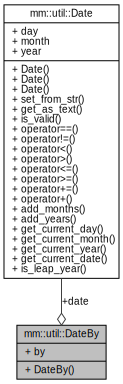
\includegraphics[width=195pt]{d2/d03/structmm_1_1util_1_1_date_by__coll__graph}
\end{center}
\end{figure}
\subsection*{Membri pubblici}
\begin{DoxyCompactItemize}
\item 
\hyperlink{structmm_1_1util_1_1_date_by_a2e30c048476714b88489a1a90a1f976c}{Date\+By} (\hyperlink{structmm_1_1util_1_1_date}{Date} \hyperlink{structmm_1_1util_1_1_date_by_a4adb77c6560794be119e39b374498b68}{date}=\{\}, std\+::string \hyperlink{structmm_1_1util_1_1_date_by_ae431f5029222a6ec9293c4c4564834f3}{by}=\char`\"{}\char`\"{})
\end{DoxyCompactItemize}
\subsection*{Attributi pubblici}
\begin{DoxyCompactItemize}
\item 
\hyperlink{structmm_1_1util_1_1_date}{Date} \hyperlink{structmm_1_1util_1_1_date_by_a4adb77c6560794be119e39b374498b68}{date}
\item 
std\+::string \hyperlink{structmm_1_1util_1_1_date_by_ae431f5029222a6ec9293c4c4564834f3}{by}
\end{DoxyCompactItemize}
\subsection*{Friend}
\begin{DoxyCompactItemize}
\item 
std\+::ostream \& \hyperlink{structmm_1_1util_1_1_date_by_aee4b77cd66c6fc86b3346dcb9fc9992a}{operator$<$$<$} (std\+::ostream \&os, const \hyperlink{structmm_1_1util_1_1_date_by}{Date\+By} \&\hyperlink{structmm_1_1util_1_1_date_by_ae431f5029222a6ec9293c4c4564834f3}{by})
\end{DoxyCompactItemize}


\subsection{Documentazione dei costruttori e dei distruttori}
\mbox{\Hypertarget{structmm_1_1util_1_1_date_by_a2e30c048476714b88489a1a90a1f976c}\label{structmm_1_1util_1_1_date_by_a2e30c048476714b88489a1a90a1f976c}} 
\index{mm\+::util\+::\+Date\+By@{mm\+::util\+::\+Date\+By}!Date\+By@{Date\+By}}
\index{Date\+By@{Date\+By}!mm\+::util\+::\+Date\+By@{mm\+::util\+::\+Date\+By}}
\subsubsection{\texorpdfstring{Date\+By()}{DateBy()}}
{\footnotesize\ttfamily mm\+::util\+::\+Date\+By\+::\+Date\+By (\begin{DoxyParamCaption}\item[{\hyperlink{structmm_1_1util_1_1_date}{Date}}]{date = {\ttfamily \{\}},  }\item[{std\+::string}]{by = {\ttfamily \char`\"{}\char`\"{}} }\end{DoxyParamCaption})}



\subsection{Documentazione dei friend e delle funzioni collegate}
\mbox{\Hypertarget{structmm_1_1util_1_1_date_by_aee4b77cd66c6fc86b3346dcb9fc9992a}\label{structmm_1_1util_1_1_date_by_aee4b77cd66c6fc86b3346dcb9fc9992a}} 
\index{mm\+::util\+::\+Date\+By@{mm\+::util\+::\+Date\+By}!operator$<$$<$@{operator$<$$<$}}
\index{operator$<$$<$@{operator$<$$<$}!mm\+::util\+::\+Date\+By@{mm\+::util\+::\+Date\+By}}
\subsubsection{\texorpdfstring{operator$<$$<$}{operator<<}}
{\footnotesize\ttfamily std\+::ostream\& operator$<$$<$ (\begin{DoxyParamCaption}\item[{std\+::ostream \&}]{os,  }\item[{const \hyperlink{structmm_1_1util_1_1_date_by}{Date\+By} \&}]{by }\end{DoxyParamCaption})\hspace{0.3cm}{\ttfamily [friend]}}



\subsection{Documentazione dei membri dato}
\mbox{\Hypertarget{structmm_1_1util_1_1_date_by_ae431f5029222a6ec9293c4c4564834f3}\label{structmm_1_1util_1_1_date_by_ae431f5029222a6ec9293c4c4564834f3}} 
\index{mm\+::util\+::\+Date\+By@{mm\+::util\+::\+Date\+By}!by@{by}}
\index{by@{by}!mm\+::util\+::\+Date\+By@{mm\+::util\+::\+Date\+By}}
\subsubsection{\texorpdfstring{by}{by}}
{\footnotesize\ttfamily std\+::string mm\+::util\+::\+Date\+By\+::by}

\mbox{\Hypertarget{structmm_1_1util_1_1_date_by_a4adb77c6560794be119e39b374498b68}\label{structmm_1_1util_1_1_date_by_a4adb77c6560794be119e39b374498b68}} 
\index{mm\+::util\+::\+Date\+By@{mm\+::util\+::\+Date\+By}!date@{date}}
\index{date@{date}!mm\+::util\+::\+Date\+By@{mm\+::util\+::\+Date\+By}}
\subsubsection{\texorpdfstring{date}{date}}
{\footnotesize\ttfamily \hyperlink{structmm_1_1util_1_1_date}{Date} mm\+::util\+::\+Date\+By\+::date}



La documentazione per questa struct è stata generata a partire dai seguenti file\+:\begin{DoxyCompactItemize}
\item 
code/utils/\hyperlink{_date_by_8hpp}{Date\+By.\+hpp}\item 
code/utils/\hyperlink{_date_by_8cpp}{Date\+By.\+cpp}\end{DoxyCompactItemize}

\hypertarget{structmm_1_1_date_controller}{}\section{Riferimenti per la struct mm\+:\+:Date\+Controller}
\label{structmm_1_1_date_controller}\index{mm\+::\+Date\+Controller@{mm\+::\+Date\+Controller}}


{\ttfamily \#include $<$Widgets.\+hpp$>$}



Diagramma delle classi per mm\+:\+:Date\+Controller
\nopagebreak
\begin{figure}[H]
\begin{center}
\leavevmode
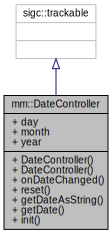
\includegraphics[width=184pt]{db/db8/structmm_1_1_date_controller__inherit__graph}
\end{center}
\end{figure}


Diagramma di collaborazione per mm\+:\+:Date\+Controller\+:
\nopagebreak
\begin{figure}[H]
\begin{center}
\leavevmode
\includegraphics[width=184pt]{d0/d40/structmm_1_1_date_controller__coll__graph}
\end{center}
\end{figure}
\subsection*{Membri pubblici}
\begin{DoxyCompactItemize}
\item 
\mbox{\hyperlink{structmm_1_1_date_controller_a3244d913ab9d7b96e9617f8711e34bd8}{Date\+Controller}} ()=delete
\item 
\mbox{\hyperlink{structmm_1_1_date_controller_a591167277348214a72634a4bbc9272ad}{Date\+Controller}} (const std\+::string \&day\+Id, const std\+::string \&month\+Id, const std\+::string \&year\+Id)
\item 
void \mbox{\hyperlink{structmm_1_1_date_controller_a7474c420c78178ee6ee6a2e66c16803f}{on\+Date\+Changed}} ()
\item 
void \mbox{\hyperlink{structmm_1_1_date_controller_a9e09c31aa55c3389c6919c716bb8b0dc}{reset}} ()
\item 
std\+::string \mbox{\hyperlink{structmm_1_1_date_controller_a8ebf6bda6699414521e4e299fd59e843}{get\+Date\+As\+String}} ()
\item 
\mbox{\hyperlink{structmm_1_1util_1_1_date}{util\+::\+Date}} \mbox{\hyperlink{structmm_1_1_date_controller_aa3c0122bfcc36e8d8b43c8ca7ca76197}{get\+Date}} ()
\item 
void \mbox{\hyperlink{structmm_1_1_date_controller_aa7f999d2d5afec5c6724f92cf2856171}{init}} ()
\end{DoxyCompactItemize}
\subsection*{Attributi pubblici}
\begin{DoxyCompactItemize}
\item 
Gtk\+::\+Combo\+Box\+Text $\ast$ \mbox{\hyperlink{structmm_1_1_date_controller_a332df89b4a88fe3ace3d6d86934a575d}{day}}
\item 
Gtk\+::\+Combo\+Box\+Text $\ast$ \mbox{\hyperlink{structmm_1_1_date_controller_a1e7373cef0b00e63343ef9d30a1e80c5}{month}}
\item 
Gtk\+::\+Combo\+Box\+Text $\ast$ \mbox{\hyperlink{structmm_1_1_date_controller_a36179406cda47b8c18d1a84945a5e61c}{year}}
\end{DoxyCompactItemize}


\subsection{Documentazione dei costruttori e dei distruttori}
\mbox{\Hypertarget{structmm_1_1_date_controller_a3244d913ab9d7b96e9617f8711e34bd8}\label{structmm_1_1_date_controller_a3244d913ab9d7b96e9617f8711e34bd8}} 
\index{mm\+::\+Date\+Controller@{mm\+::\+Date\+Controller}!Date\+Controller@{Date\+Controller}}
\index{Date\+Controller@{Date\+Controller}!mm\+::\+Date\+Controller@{mm\+::\+Date\+Controller}}
\subsubsection{\texorpdfstring{Date\+Controller()}{DateController()}\hspace{0.1cm}{\footnotesize\ttfamily [1/2]}}
{\footnotesize\ttfamily mm\+::\+Date\+Controller\+::\+Date\+Controller (\begin{DoxyParamCaption}{ }\end{DoxyParamCaption})\hspace{0.3cm}{\ttfamily [delete]}}

\mbox{\Hypertarget{structmm_1_1_date_controller_a591167277348214a72634a4bbc9272ad}\label{structmm_1_1_date_controller_a591167277348214a72634a4bbc9272ad}} 
\index{mm\+::\+Date\+Controller@{mm\+::\+Date\+Controller}!Date\+Controller@{Date\+Controller}}
\index{Date\+Controller@{Date\+Controller}!mm\+::\+Date\+Controller@{mm\+::\+Date\+Controller}}
\subsubsection{\texorpdfstring{Date\+Controller()}{DateController()}\hspace{0.1cm}{\footnotesize\ttfamily [2/2]}}
{\footnotesize\ttfamily mm\+::\+Date\+Controller\+::\+Date\+Controller (\begin{DoxyParamCaption}\item[{const std\+::string \&}]{day\+Id,  }\item[{const std\+::string \&}]{month\+Id,  }\item[{const std\+::string \&}]{year\+Id }\end{DoxyParamCaption})}



\subsection{Documentazione delle funzioni membro}
\mbox{\Hypertarget{structmm_1_1_date_controller_aa3c0122bfcc36e8d8b43c8ca7ca76197}\label{structmm_1_1_date_controller_aa3c0122bfcc36e8d8b43c8ca7ca76197}} 
\index{mm\+::\+Date\+Controller@{mm\+::\+Date\+Controller}!get\+Date@{get\+Date}}
\index{get\+Date@{get\+Date}!mm\+::\+Date\+Controller@{mm\+::\+Date\+Controller}}
\subsubsection{\texorpdfstring{get\+Date()}{getDate()}}
{\footnotesize\ttfamily \mbox{\hyperlink{structmm_1_1util_1_1_date}{mm\+::util\+::\+Date}} mm\+::\+Date\+Controller\+::get\+Date (\begin{DoxyParamCaption}{ }\end{DoxyParamCaption})}

\mbox{\Hypertarget{structmm_1_1_date_controller_a8ebf6bda6699414521e4e299fd59e843}\label{structmm_1_1_date_controller_a8ebf6bda6699414521e4e299fd59e843}} 
\index{mm\+::\+Date\+Controller@{mm\+::\+Date\+Controller}!get\+Date\+As\+String@{get\+Date\+As\+String}}
\index{get\+Date\+As\+String@{get\+Date\+As\+String}!mm\+::\+Date\+Controller@{mm\+::\+Date\+Controller}}
\subsubsection{\texorpdfstring{get\+Date\+As\+String()}{getDateAsString()}}
{\footnotesize\ttfamily std\+::string mm\+::\+Date\+Controller\+::get\+Date\+As\+String (\begin{DoxyParamCaption}{ }\end{DoxyParamCaption})\hspace{0.3cm}{\ttfamily [inline]}}

\mbox{\Hypertarget{structmm_1_1_date_controller_aa7f999d2d5afec5c6724f92cf2856171}\label{structmm_1_1_date_controller_aa7f999d2d5afec5c6724f92cf2856171}} 
\index{mm\+::\+Date\+Controller@{mm\+::\+Date\+Controller}!init@{init}}
\index{init@{init}!mm\+::\+Date\+Controller@{mm\+::\+Date\+Controller}}
\subsubsection{\texorpdfstring{init()}{init()}}
{\footnotesize\ttfamily void mm\+::\+Date\+Controller\+::init (\begin{DoxyParamCaption}{ }\end{DoxyParamCaption})}

\mbox{\Hypertarget{structmm_1_1_date_controller_a7474c420c78178ee6ee6a2e66c16803f}\label{structmm_1_1_date_controller_a7474c420c78178ee6ee6a2e66c16803f}} 
\index{mm\+::\+Date\+Controller@{mm\+::\+Date\+Controller}!on\+Date\+Changed@{on\+Date\+Changed}}
\index{on\+Date\+Changed@{on\+Date\+Changed}!mm\+::\+Date\+Controller@{mm\+::\+Date\+Controller}}
\subsubsection{\texorpdfstring{on\+Date\+Changed()}{onDateChanged()}}
{\footnotesize\ttfamily void mm\+::\+Date\+Controller\+::on\+Date\+Changed (\begin{DoxyParamCaption}{ }\end{DoxyParamCaption})}

\mbox{\Hypertarget{structmm_1_1_date_controller_a9e09c31aa55c3389c6919c716bb8b0dc}\label{structmm_1_1_date_controller_a9e09c31aa55c3389c6919c716bb8b0dc}} 
\index{mm\+::\+Date\+Controller@{mm\+::\+Date\+Controller}!reset@{reset}}
\index{reset@{reset}!mm\+::\+Date\+Controller@{mm\+::\+Date\+Controller}}
\subsubsection{\texorpdfstring{reset()}{reset()}}
{\footnotesize\ttfamily void mm\+::\+Date\+Controller\+::reset (\begin{DoxyParamCaption}{ }\end{DoxyParamCaption})}



\subsection{Documentazione dei membri dato}
\mbox{\Hypertarget{structmm_1_1_date_controller_a332df89b4a88fe3ace3d6d86934a575d}\label{structmm_1_1_date_controller_a332df89b4a88fe3ace3d6d86934a575d}} 
\index{mm\+::\+Date\+Controller@{mm\+::\+Date\+Controller}!day@{day}}
\index{day@{day}!mm\+::\+Date\+Controller@{mm\+::\+Date\+Controller}}
\subsubsection{\texorpdfstring{day}{day}}
{\footnotesize\ttfamily Gtk\+::\+Combo\+Box\+Text$\ast$ mm\+::\+Date\+Controller\+::day}

\mbox{\Hypertarget{structmm_1_1_date_controller_a1e7373cef0b00e63343ef9d30a1e80c5}\label{structmm_1_1_date_controller_a1e7373cef0b00e63343ef9d30a1e80c5}} 
\index{mm\+::\+Date\+Controller@{mm\+::\+Date\+Controller}!month@{month}}
\index{month@{month}!mm\+::\+Date\+Controller@{mm\+::\+Date\+Controller}}
\subsubsection{\texorpdfstring{month}{month}}
{\footnotesize\ttfamily Gtk\+::\+Combo\+Box\+Text$\ast$ mm\+::\+Date\+Controller\+::month}

\mbox{\Hypertarget{structmm_1_1_date_controller_a36179406cda47b8c18d1a84945a5e61c}\label{structmm_1_1_date_controller_a36179406cda47b8c18d1a84945a5e61c}} 
\index{mm\+::\+Date\+Controller@{mm\+::\+Date\+Controller}!year@{year}}
\index{year@{year}!mm\+::\+Date\+Controller@{mm\+::\+Date\+Controller}}
\subsubsection{\texorpdfstring{year}{year}}
{\footnotesize\ttfamily Gtk\+::\+Combo\+Box\+Text$\ast$ mm\+::\+Date\+Controller\+::year}



La documentazione per questa struct è stata generata a partire dai seguenti file\+:\begin{DoxyCompactItemize}
\item 
code/gui/\mbox{\hyperlink{_widgets_8hpp}{Widgets.\+hpp}}\item 
code/gui/\mbox{\hyperlink{_widgets_8cpp}{Widgets.\+cpp}}\end{DoxyCompactItemize}

\hypertarget{classmm_1_1_d_b_master}{}\section{Riferimenti per la classe mm\+:\+:D\+B\+Master}
\label{classmm_1_1_d_b_master}\index{mm\+::\+D\+B\+Master@{mm\+::\+D\+B\+Master}}


Singleton che rappresenta il database, contiene tutte le funzioni necessarie per scrivere un oggetto di tipo derivato da \hyperlink{classmm_1_1_i_serializable}{I\+Serializable} e per leggerlo. Nasconde le chiamate alle A\+PI C di sqlite3.  




{\ttfamily \#include $<$D\+B\+Master.\+hpp$>$}



Diagramma di collaborazione per mm\+:\+:D\+B\+Master\+:\nopagebreak
\begin{figure}[H]
\begin{center}
\leavevmode
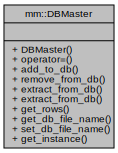
\includegraphics[width=191pt]{d7/d6f/classmm_1_1_d_b_master__coll__graph}
\end{center}
\end{figure}
\subsection*{Membri pubblici}
\begin{DoxyCompactItemize}
\item 
\hyperlink{classmm_1_1_d_b_master_a7571cbb3fe77a491d57595ec9bc86abf}{D\+B\+Master} (const \hyperlink{classmm_1_1_d_b_master}{D\+B\+Master} \&old)=delete
\item 
const \hyperlink{classmm_1_1_d_b_master}{D\+B\+Master} \& \hyperlink{classmm_1_1_d_b_master_af556b0856b79cb8bff3da0565badeac0}{operator=} (const \hyperlink{classmm_1_1_d_b_master}{D\+B\+Master} \&old)=delete
\item 
void \hyperlink{classmm_1_1_d_b_master_a187988c8741d0a2c5806919b8d672af0}{add\+\_\+to\+\_\+db} (const \hyperlink{classmm_1_1_i_serializable}{I\+Serializable} \&obj)
\begin{DoxyCompactList}\small\item\em aggiunge un oggetto serializzabile ad database \end{DoxyCompactList}\item 
void \hyperlink{classmm_1_1_d_b_master_a4d5d51bf4b3437294a52fcd3747520d3}{remove\+\_\+from\+\_\+db} (const \hyperlink{classmm_1_1_i_serializable}{I\+Serializable} \&obj)
\begin{DoxyCompactList}\small\item\em rimuove un oggetto serializzabile dal database \end{DoxyCompactList}\item 
void \hyperlink{classmm_1_1_d_b_master_a9e8092b67a249a273668ad042a4084e2}{extract\+\_\+from\+\_\+db} (\hyperlink{classmm_1_1_i_serializable}{I\+Serializable} \&obj, initializer\+\_\+list$<$ \hyperlink{structmm_1_1_serialized}{Serialized} $>$ ids)
\begin{DoxyCompactList}\small\item\em estrae un oggetto serializzabile dal database \end{DoxyCompactList}\item 
void \hyperlink{classmm_1_1_d_b_master_a68c25d223994752e8b4d6156a23651f2}{extract\+\_\+from\+\_\+db} (\hyperlink{classmm_1_1_i_serializable}{I\+Serializable} \&obj, const \hyperlink{structmm_1_1_serialized}{Serialized} \&id)
\begin{DoxyCompactList}\small\item\em shortcut per la versione che accetta un initializer\+\_\+list per poterla chiamare con un solo id in modo semplice \end{DoxyCompactList}\item 
vector$<$ map$<$ string, \hyperlink{structmm_1_1_serialized}{Serialized} $>$ $>$ \hyperlink{classmm_1_1_d_b_master_aef9d7063da9d7b4e0fb0a20a6d06368f}{get\+\_\+rows} (string table\+\_\+name, string id\+\_\+name=\char`\"{}\char`\"{}, \hyperlink{structmm_1_1_serialized}{Serialized} id=\char`\"{}\char`\"{})
\begin{DoxyCompactList}\small\item\em estrae un insieme di righe da una tabella \end{DoxyCompactList}\end{DoxyCompactItemize}
\subsection*{Membri pubblici statici}
\begin{DoxyCompactItemize}
\item 
static const string \& \hyperlink{classmm_1_1_d_b_master_a65586b91e19e610db40ef1d6e81cfd4a}{get\+\_\+db\+\_\+file\+\_\+name} ()
\item 
static void \hyperlink{classmm_1_1_d_b_master_a3346d25779e18ed7ad70eed0d89347e9}{set\+\_\+db\+\_\+file\+\_\+name} (const string \&db\+\_\+file\+\_\+name)
\begin{DoxyCompactList}\small\item\em imposta il path nel quale trovare il database \end{DoxyCompactList}\item 
static \hyperlink{classmm_1_1_d_b_master}{D\+B\+Master} \& \hyperlink{classmm_1_1_d_b_master_a1f3b04e515b1999d3900353c0054f498}{get\+\_\+instance} () noexcept(false)
\begin{DoxyCompactList}\small\item\em restituisce una reference (non costante) all\textquotesingle{}oggetto db \end{DoxyCompactList}\end{DoxyCompactItemize}


\subsection{Descrizione dettagliata}
Singleton che rappresenta il database, contiene tutte le funzioni necessarie per scrivere un oggetto di tipo derivato da \hyperlink{classmm_1_1_i_serializable}{I\+Serializable} e per leggerlo. Nasconde le chiamate alle A\+PI C di sqlite3. 

È un singleton di tipo lazy. Prima di chiamare get\+\_\+instance è sempre necessario informare la classe del path del database chiamando set\+\_\+db\+\_\+name 

\subsection{Documentazione dei costruttori e dei distruttori}
\mbox{\Hypertarget{classmm_1_1_d_b_master_a7571cbb3fe77a491d57595ec9bc86abf}\label{classmm_1_1_d_b_master_a7571cbb3fe77a491d57595ec9bc86abf}} 
\index{mm\+::\+D\+B\+Master@{mm\+::\+D\+B\+Master}!D\+B\+Master@{D\+B\+Master}}
\index{D\+B\+Master@{D\+B\+Master}!mm\+::\+D\+B\+Master@{mm\+::\+D\+B\+Master}}
\subsubsection{\texorpdfstring{D\+B\+Master()}{DBMaster()}}
{\footnotesize\ttfamily mm\+::\+D\+B\+Master\+::\+D\+B\+Master (\begin{DoxyParamCaption}\item[{const \hyperlink{classmm_1_1_d_b_master}{D\+B\+Master} \&}]{old }\end{DoxyParamCaption})\hspace{0.3cm}{\ttfamily [delete]}}



\subsection{Documentazione delle funzioni membro}
\mbox{\Hypertarget{classmm_1_1_d_b_master_a187988c8741d0a2c5806919b8d672af0}\label{classmm_1_1_d_b_master_a187988c8741d0a2c5806919b8d672af0}} 
\index{mm\+::\+D\+B\+Master@{mm\+::\+D\+B\+Master}!add\+\_\+to\+\_\+db@{add\+\_\+to\+\_\+db}}
\index{add\+\_\+to\+\_\+db@{add\+\_\+to\+\_\+db}!mm\+::\+D\+B\+Master@{mm\+::\+D\+B\+Master}}
\subsubsection{\texorpdfstring{add\+\_\+to\+\_\+db()}{add\_to\_db()}}
{\footnotesize\ttfamily void mm\+::\+D\+B\+Master\+::add\+\_\+to\+\_\+db (\begin{DoxyParamCaption}\item[{const \hyperlink{classmm_1_1_i_serializable}{I\+Serializable} \&}]{obj }\end{DoxyParamCaption})}



aggiunge un oggetto serializzabile ad database 

Questo metodo può eseguire o un U\+P\+D\+A\+TE o un I\+N\+S\+E\+RT a seconda che l\textquotesingle{}oggetto sia già presente o meno nel db. Può lanciare eccezioni del tipo std\+::runtime error in caso di errore


\begin{DoxyParams}[1]{Parametri}
\mbox{\tt in}  & {\em obj} & un oggetto serializzabile (che estende la classe \hyperlink{classmm_1_1_i_serializable}{I\+Serializable}) \\
\hline
\end{DoxyParams}
\mbox{\Hypertarget{classmm_1_1_d_b_master_a9e8092b67a249a273668ad042a4084e2}\label{classmm_1_1_d_b_master_a9e8092b67a249a273668ad042a4084e2}} 
\index{mm\+::\+D\+B\+Master@{mm\+::\+D\+B\+Master}!extract\+\_\+from\+\_\+db@{extract\+\_\+from\+\_\+db}}
\index{extract\+\_\+from\+\_\+db@{extract\+\_\+from\+\_\+db}!mm\+::\+D\+B\+Master@{mm\+::\+D\+B\+Master}}
\subsubsection{\texorpdfstring{extract\+\_\+from\+\_\+db()}{extract\_from\_db()}\hspace{0.1cm}{\footnotesize\ttfamily [1/2]}}
{\footnotesize\ttfamily void mm\+::\+D\+B\+Master\+::extract\+\_\+from\+\_\+db (\begin{DoxyParamCaption}\item[{\hyperlink{classmm_1_1_i_serializable}{mm\+::\+I\+Serializable} \&}]{obj,  }\item[{initializer\+\_\+list$<$ \hyperlink{structmm_1_1_serialized}{Serialized} $>$}]{ids }\end{DoxyParamCaption})}



estrae un oggetto serializzabile dal database 

Può lanciare eccezioni di tipo std\+::runtime\+\_\+error in caso di errore di comunicazione col database oppure può lanciare eccezioni del tipo record\+\_\+no\+\_\+found\+\_\+error nel caso in cui l\textquotesingle{}oggetto con gli id specificati non sia presente nel db

N.\+B. l\textquotesingle{}oggetto passato in obj viene modificato e qualsiasi dato in esso contenuto viene sovrascritto


\begin{DoxyParams}[1]{Parametri}
\mbox{\tt out}  & {\em obj} & un oggetto serializzabile (che estende la classe \hyperlink{classmm_1_1_i_serializable}{I\+Serializable}) in cui salvare i dati del db \\
\hline
\mbox{\tt in}  & {\em ids} & lista di oggetti di tipo \hyperlink{structmm_1_1_serialized}{Serialized} che servono da primary key nel database \\
\hline
\end{DoxyParams}
\mbox{\Hypertarget{classmm_1_1_d_b_master_a68c25d223994752e8b4d6156a23651f2}\label{classmm_1_1_d_b_master_a68c25d223994752e8b4d6156a23651f2}} 
\index{mm\+::\+D\+B\+Master@{mm\+::\+D\+B\+Master}!extract\+\_\+from\+\_\+db@{extract\+\_\+from\+\_\+db}}
\index{extract\+\_\+from\+\_\+db@{extract\+\_\+from\+\_\+db}!mm\+::\+D\+B\+Master@{mm\+::\+D\+B\+Master}}
\subsubsection{\texorpdfstring{extract\+\_\+from\+\_\+db()}{extract\_from\_db()}\hspace{0.1cm}{\footnotesize\ttfamily [2/2]}}
{\footnotesize\ttfamily void mm\+::\+D\+B\+Master\+::extract\+\_\+from\+\_\+db (\begin{DoxyParamCaption}\item[{\hyperlink{classmm_1_1_i_serializable}{mm\+::\+I\+Serializable} \&}]{obj,  }\item[{const \hyperlink{structmm_1_1_serialized}{Serialized} \&}]{id }\end{DoxyParamCaption})}



shortcut per la versione che accetta un initializer\+\_\+list per poterla chiamare con un solo id in modo semplice 

\mbox{\Hypertarget{classmm_1_1_d_b_master_a65586b91e19e610db40ef1d6e81cfd4a}\label{classmm_1_1_d_b_master_a65586b91e19e610db40ef1d6e81cfd4a}} 
\index{mm\+::\+D\+B\+Master@{mm\+::\+D\+B\+Master}!get\+\_\+db\+\_\+file\+\_\+name@{get\+\_\+db\+\_\+file\+\_\+name}}
\index{get\+\_\+db\+\_\+file\+\_\+name@{get\+\_\+db\+\_\+file\+\_\+name}!mm\+::\+D\+B\+Master@{mm\+::\+D\+B\+Master}}
\subsubsection{\texorpdfstring{get\+\_\+db\+\_\+file\+\_\+name()}{get\_db\_file\_name()}}
{\footnotesize\ttfamily const std\+::string \& mm\+::\+D\+B\+Master\+::get\+\_\+db\+\_\+file\+\_\+name (\begin{DoxyParamCaption}{ }\end{DoxyParamCaption})\hspace{0.3cm}{\ttfamily [static]}}

\mbox{\Hypertarget{classmm_1_1_d_b_master_a1f3b04e515b1999d3900353c0054f498}\label{classmm_1_1_d_b_master_a1f3b04e515b1999d3900353c0054f498}} 
\index{mm\+::\+D\+B\+Master@{mm\+::\+D\+B\+Master}!get\+\_\+instance@{get\+\_\+instance}}
\index{get\+\_\+instance@{get\+\_\+instance}!mm\+::\+D\+B\+Master@{mm\+::\+D\+B\+Master}}
\subsubsection{\texorpdfstring{get\+\_\+instance()}{get\_instance()}}
{\footnotesize\ttfamily \hyperlink{classmm_1_1_d_b_master}{mm\+::\+D\+B\+Master} \& mm\+::\+D\+B\+Master\+::get\+\_\+instance (\begin{DoxyParamCaption}{ }\end{DoxyParamCaption})\hspace{0.3cm}{\ttfamily [static]}, {\ttfamily [noexcept]}}



restituisce una reference (non costante) all\textquotesingle{}oggetto db 

Siccome il distruttore è privato non è possibile che quella reference venga distrutta al di fuori della classe

\begin{DoxyReturn}{Restituisce}
reference ad un oggetto \hyperlink{classmm_1_1_d_b_master}{D\+B\+Master} 
\end{DoxyReturn}
\mbox{\Hypertarget{classmm_1_1_d_b_master_aef9d7063da9d7b4e0fb0a20a6d06368f}\label{classmm_1_1_d_b_master_aef9d7063da9d7b4e0fb0a20a6d06368f}} 
\index{mm\+::\+D\+B\+Master@{mm\+::\+D\+B\+Master}!get\+\_\+rows@{get\+\_\+rows}}
\index{get\+\_\+rows@{get\+\_\+rows}!mm\+::\+D\+B\+Master@{mm\+::\+D\+B\+Master}}
\subsubsection{\texorpdfstring{get\+\_\+rows()}{get\_rows()}}
{\footnotesize\ttfamily vector$<$ map$<$ string, \hyperlink{structmm_1_1_serialized}{mm\+::\+Serialized} $>$ $>$ mm\+::\+D\+B\+Master\+::get\+\_\+rows (\begin{DoxyParamCaption}\item[{string}]{table\+\_\+name,  }\item[{string}]{id\+\_\+name = {\ttfamily \char`\"{}\char`\"{}},  }\item[{\hyperlink{structmm_1_1_serialized}{mm\+::\+Serialized}}]{id = {\ttfamily \char`\"{}\char`\"{}} }\end{DoxyParamCaption})}



estrae un insieme di righe da una tabella 

Se non vengono passati i parametri id\+\_\+name e id il metodo ritorna tutte le righe della tabella altrimenti ritorna solo le righe che hanno quell\textquotesingle{}id e quell\textquotesingle{}id\+\_\+name


\begin{DoxyParams}[1]{Parametri}
\mbox{\tt in}  & {\em table\+\_\+name} & Parametro obbligatorio che contiene il nome della tabella dal quale estrarre le righe \\
\hline
\mbox{\tt in}  & {\em id\+\_\+name} & Parametro opzionale che contiene il nome della colonna presa come id \\
\hline
\mbox{\tt in}  & {\em id} & Parametro opzionale che contiene il valore che deve essere contenuto nella colonna id\+\_\+name\\
\hline
\end{DoxyParams}
\begin{DoxyReturn}{Restituisce}
Un vettore di mappe di stringe e serialized ogni mappa rappresenta una riga dove una colonna è identificata dalla stringa ed il contenuto dall\textquotesingle{}oggetto serialized 
\end{DoxyReturn}
\mbox{\Hypertarget{classmm_1_1_d_b_master_af556b0856b79cb8bff3da0565badeac0}\label{classmm_1_1_d_b_master_af556b0856b79cb8bff3da0565badeac0}} 
\index{mm\+::\+D\+B\+Master@{mm\+::\+D\+B\+Master}!operator=@{operator=}}
\index{operator=@{operator=}!mm\+::\+D\+B\+Master@{mm\+::\+D\+B\+Master}}
\subsubsection{\texorpdfstring{operator=()}{operator=()}}
{\footnotesize\ttfamily const \hyperlink{classmm_1_1_d_b_master}{D\+B\+Master}\& mm\+::\+D\+B\+Master\+::operator= (\begin{DoxyParamCaption}\item[{const \hyperlink{classmm_1_1_d_b_master}{D\+B\+Master} \&}]{old }\end{DoxyParamCaption})\hspace{0.3cm}{\ttfamily [delete]}}

\mbox{\Hypertarget{classmm_1_1_d_b_master_a4d5d51bf4b3437294a52fcd3747520d3}\label{classmm_1_1_d_b_master_a4d5d51bf4b3437294a52fcd3747520d3}} 
\index{mm\+::\+D\+B\+Master@{mm\+::\+D\+B\+Master}!remove\+\_\+from\+\_\+db@{remove\+\_\+from\+\_\+db}}
\index{remove\+\_\+from\+\_\+db@{remove\+\_\+from\+\_\+db}!mm\+::\+D\+B\+Master@{mm\+::\+D\+B\+Master}}
\subsubsection{\texorpdfstring{remove\+\_\+from\+\_\+db()}{remove\_from\_db()}}
{\footnotesize\ttfamily void mm\+::\+D\+B\+Master\+::remove\+\_\+from\+\_\+db (\begin{DoxyParamCaption}\item[{const \hyperlink{classmm_1_1_i_serializable}{I\+Serializable} \&}]{obj }\end{DoxyParamCaption})}



rimuove un oggetto serializzabile dal database 

Può lanciare eccezioni di tipo std\+::runtime\+\_\+error in caso di errore di comunicazione col database

N.\+B. sia che l\textquotesingle{}operazione vada a buon fine o meno l\textquotesingle{}oggetto non viene modificato


\begin{DoxyParams}[1]{Parametri}
\mbox{\tt in}  & {\em obj} & un oggetto serializzabile (che estende la classe \hyperlink{classmm_1_1_i_serializable}{I\+Serializable}) \\
\hline
\end{DoxyParams}
\mbox{\Hypertarget{classmm_1_1_d_b_master_a3346d25779e18ed7ad70eed0d89347e9}\label{classmm_1_1_d_b_master_a3346d25779e18ed7ad70eed0d89347e9}} 
\index{mm\+::\+D\+B\+Master@{mm\+::\+D\+B\+Master}!set\+\_\+db\+\_\+file\+\_\+name@{set\+\_\+db\+\_\+file\+\_\+name}}
\index{set\+\_\+db\+\_\+file\+\_\+name@{set\+\_\+db\+\_\+file\+\_\+name}!mm\+::\+D\+B\+Master@{mm\+::\+D\+B\+Master}}
\subsubsection{\texorpdfstring{set\+\_\+db\+\_\+file\+\_\+name()}{set\_db\_file\_name()}}
{\footnotesize\ttfamily void mm\+::\+D\+B\+Master\+::set\+\_\+db\+\_\+file\+\_\+name (\begin{DoxyParamCaption}\item[{const string \&}]{db\+\_\+file\+\_\+name }\end{DoxyParamCaption})\hspace{0.3cm}{\ttfamily [static]}}



imposta il path nel quale trovare il database 

Questa funzione deve sempre essere chiamata prima di una qualsiasi chiamata a get\+\_\+instance 
\begin{DoxyParams}[1]{Parametri}
\mbox{\tt in}  & {\em db\+\_\+file\+\_\+name} & \\
\hline
\end{DoxyParams}


La documentazione per questa classe è stata generata a partire dai seguenti file\+:\begin{DoxyCompactItemize}
\item 
code/\hyperlink{_d_b_master_8hpp}{D\+B\+Master.\+hpp}\item 
code/\hyperlink{_d_b_master_8cpp}{D\+B\+Master.\+cpp}\end{DoxyCompactItemize}

\hypertarget{classmm_1_1_dialog}{}\section{Riferimenti per la classe mm\+:\+:Dialog}
\label{classmm_1_1_dialog}\index{mm\+::\+Dialog@{mm\+::\+Dialog}}


{\ttfamily \#include $<$Dialog.\+hpp$>$}



Diagramma delle classi per mm\+:\+:Dialog\nopagebreak
\begin{figure}[H]
\begin{center}
\leavevmode
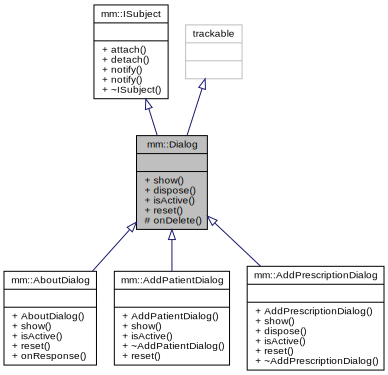
\includegraphics[width=350pt]{d8/dfd/classmm_1_1_dialog__inherit__graph}
\end{center}
\end{figure}


Diagramma di collaborazione per mm\+:\+:Dialog\+:\nopagebreak
\begin{figure}[H]
\begin{center}
\leavevmode
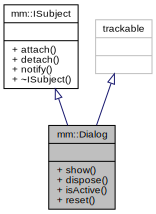
\includegraphics[width=228pt]{d7/d10/classmm_1_1_dialog__coll__graph}
\end{center}
\end{figure}
\subsection*{Membri pubblici}
\begin{DoxyCompactItemize}
\item 
virtual void \hyperlink{classmm_1_1_dialog_afda4b0dc7c0ac027c4b8fdb95713700f}{show} ()=0
\item 
virtual void \hyperlink{classmm_1_1_dialog_a3f2e361836af48ee3808f4dd6e4f8e48}{dispose} ()=0
\item 
virtual bool \hyperlink{classmm_1_1_dialog_a22abaf4e90b6fdca5c20039f6b9e15ac}{is\+Active} ()=0
\item 
virtual void \hyperlink{classmm_1_1_dialog_abe6e5ac072c12c06971f60491f079d80}{reset} ()=0
\end{DoxyCompactItemize}


\subsection{Documentazione delle funzioni membro}
\mbox{\Hypertarget{classmm_1_1_dialog_a3f2e361836af48ee3808f4dd6e4f8e48}\label{classmm_1_1_dialog_a3f2e361836af48ee3808f4dd6e4f8e48}} 
\index{mm\+::\+Dialog@{mm\+::\+Dialog}!dispose@{dispose}}
\index{dispose@{dispose}!mm\+::\+Dialog@{mm\+::\+Dialog}}
\subsubsection{\texorpdfstring{dispose()}{dispose()}}
{\footnotesize\ttfamily virtual void mm\+::\+Dialog\+::dispose (\begin{DoxyParamCaption}{ }\end{DoxyParamCaption})\hspace{0.3cm}{\ttfamily [pure virtual]}}



Implementato in \hyperlink{classmm_1_1_add_prescription_dialog_aacb58c7617be2323d91cd5ab2f28e354}{mm\+::\+Add\+Prescription\+Dialog}.

\mbox{\Hypertarget{classmm_1_1_dialog_a22abaf4e90b6fdca5c20039f6b9e15ac}\label{classmm_1_1_dialog_a22abaf4e90b6fdca5c20039f6b9e15ac}} 
\index{mm\+::\+Dialog@{mm\+::\+Dialog}!is\+Active@{is\+Active}}
\index{is\+Active@{is\+Active}!mm\+::\+Dialog@{mm\+::\+Dialog}}
\subsubsection{\texorpdfstring{is\+Active()}{isActive()}}
{\footnotesize\ttfamily virtual bool mm\+::\+Dialog\+::is\+Active (\begin{DoxyParamCaption}{ }\end{DoxyParamCaption})\hspace{0.3cm}{\ttfamily [pure virtual]}}



Implementato in \hyperlink{classmm_1_1_add_prescription_dialog_a4ff93500e8fd90512dc4575147b2c910}{mm\+::\+Add\+Prescription\+Dialog}, \hyperlink{classmm_1_1_about_dialog_adc8aec0378d9d146c78eaf9a204dbf27}{mm\+::\+About\+Dialog}, e \hyperlink{classmm_1_1_add_patient_dialog_a459a8acbec1c8a5a87e00f23402d3b5d}{mm\+::\+Add\+Patient\+Dialog}.

\mbox{\Hypertarget{classmm_1_1_dialog_abe6e5ac072c12c06971f60491f079d80}\label{classmm_1_1_dialog_abe6e5ac072c12c06971f60491f079d80}} 
\index{mm\+::\+Dialog@{mm\+::\+Dialog}!reset@{reset}}
\index{reset@{reset}!mm\+::\+Dialog@{mm\+::\+Dialog}}
\subsubsection{\texorpdfstring{reset()}{reset()}}
{\footnotesize\ttfamily virtual void mm\+::\+Dialog\+::reset (\begin{DoxyParamCaption}{ }\end{DoxyParamCaption})\hspace{0.3cm}{\ttfamily [pure virtual]}}



Implementato in \hyperlink{classmm_1_1_add_patient_dialog_a64c8c2ea3b1c69a858f4eaec1854270a}{mm\+::\+Add\+Patient\+Dialog}, \hyperlink{classmm_1_1_add_prescription_dialog_a6ace04587432a197436bb04c7b68d60d}{mm\+::\+Add\+Prescription\+Dialog}, e \hyperlink{classmm_1_1_about_dialog_a21f5b0a7c9d8e43baab78e073d7ade2b}{mm\+::\+About\+Dialog}.

\mbox{\Hypertarget{classmm_1_1_dialog_afda4b0dc7c0ac027c4b8fdb95713700f}\label{classmm_1_1_dialog_afda4b0dc7c0ac027c4b8fdb95713700f}} 
\index{mm\+::\+Dialog@{mm\+::\+Dialog}!show@{show}}
\index{show@{show}!mm\+::\+Dialog@{mm\+::\+Dialog}}
\subsubsection{\texorpdfstring{show()}{show()}}
{\footnotesize\ttfamily virtual void mm\+::\+Dialog\+::show (\begin{DoxyParamCaption}{ }\end{DoxyParamCaption})\hspace{0.3cm}{\ttfamily [pure virtual]}}



Implementato in \hyperlink{classmm_1_1_about_dialog_a9e06dc12f6950b74ccf6ccece693f108}{mm\+::\+About\+Dialog}, \hyperlink{classmm_1_1_add_patient_dialog_a0247912794984eb19c43842ab9037708}{mm\+::\+Add\+Patient\+Dialog}, e \hyperlink{classmm_1_1_add_prescription_dialog_aa1c86141b2d45e141684bd99d557b8e4}{mm\+::\+Add\+Prescription\+Dialog}.



La documentazione per questa classe è stata generata a partire dal seguente file\+:\begin{DoxyCompactItemize}
\item 
code/gui/\hyperlink{_dialog_8hpp}{Dialog.\+hpp}\end{DoxyCompactItemize}

\hypertarget{classmm_1_1model_1_1_doctor}{}\section{Riferimenti per la classe mm\+:\+:model\+:\+:Doctor}
\label{classmm_1_1model_1_1_doctor}\index{mm\+::model\+::\+Doctor@{mm\+::model\+::\+Doctor}}


{\ttfamily \#include $<$Doctor.\+hpp$>$}



Diagramma delle classi per mm\+:\+:model\+:\+:Doctor\nopagebreak
\begin{figure}[H]
\begin{center}
\leavevmode
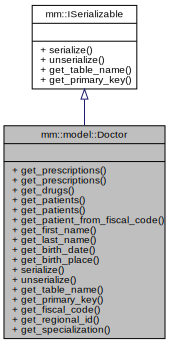
\includegraphics[width=242pt]{dd/d55/classmm_1_1model_1_1_doctor__inherit__graph}
\end{center}
\end{figure}


Diagramma di collaborazione per mm\+:\+:model\+:\+:Doctor\+:\nopagebreak
\begin{figure}[H]
\begin{center}
\leavevmode
\includegraphics[width=242pt]{da/d19/classmm_1_1model_1_1_doctor__coll__graph}
\end{center}
\end{figure}
\subsection*{Membri pubblici}
\begin{DoxyCompactItemize}
\item 
vector$<$ \hyperlink{classmm_1_1model_1_1_prescription}{model\+::\+Prescription} $>$ \hyperlink{classmm_1_1model_1_1_doctor_a16be876e8591688f3b34ca86441253a2}{get\+\_\+prescriptions} (\hyperlink{classmm_1_1model_1_1_patient}{Patient} patient, \hyperlink{structmm_1_1util_1_1_date}{util\+::\+Date} start, \hyperlink{structmm_1_1util_1_1_date}{util\+::\+Date} end)
\item 
vector$<$ \hyperlink{classmm_1_1model_1_1_prescription}{model\+::\+Prescription} $>$ \hyperlink{classmm_1_1model_1_1_doctor_a76bf6b545709c7a784e4320b11f587bf}{get\+\_\+prescriptions} (\hyperlink{classmm_1_1model_1_1_drug}{model\+::\+Drug} drug)
\item 
vector$<$ \hyperlink{classmm_1_1model_1_1_drug}{model\+::\+Drug} $>$ \hyperlink{classmm_1_1model_1_1_doctor_ace64e6e74d0e39244c349fe5570ff974}{get\+\_\+drugs} (\hyperlink{structmm_1_1util_1_1_date}{util\+::\+Date} start, \hyperlink{structmm_1_1util_1_1_date}{util\+::\+Date} end)
\item 
vector$<$ \hyperlink{classmm_1_1model_1_1_patient}{model\+::\+Patient} $>$ \& \hyperlink{classmm_1_1model_1_1_doctor_a8b761c1dfbe10348eb99c0397e811e0a}{get\+\_\+patients} ()
\item 
vector$<$ \hyperlink{classmm_1_1model_1_1_patient}{model\+::\+Patient} $>$ \hyperlink{classmm_1_1model_1_1_doctor_a989fbde1a8784d8139d8add9066ab9b1}{get\+\_\+patients} (\hyperlink{classmm_1_1model_1_1_drug}{model\+::\+Drug} drug)
\item 
\hyperlink{classmm_1_1model_1_1_patient}{model\+::\+Patient} \hyperlink{classmm_1_1model_1_1_doctor_a89aa97cb00bfa2352c2a4f276554e738}{get\+\_\+patient\+\_\+from\+\_\+fiscal\+\_\+code} (std\+::string fiscal\+\_\+code)
\item 
void \hyperlink{classmm_1_1model_1_1_doctor_a1fe35e39d290992a5f6f4a73d4fa8d50}{remove\+\_\+patient} (const \hyperlink{classmm_1_1model_1_1_patient}{Patient} \&patient)
\item 
const string \& \hyperlink{classmm_1_1model_1_1_doctor_ac33c8e6a13054d0c7aea1cf6aec4368f}{get\+\_\+first\+\_\+name} () const
\item 
const string \& \hyperlink{classmm_1_1model_1_1_doctor_a86a186641c22223ecb9951112befa3e9}{get\+\_\+last\+\_\+name} () const
\item 
const string \& \hyperlink{classmm_1_1model_1_1_doctor_afa648dfa2f37c1de94a742bd58682899}{get\+\_\+birth\+\_\+date} () const
\item 
const string \& \hyperlink{classmm_1_1model_1_1_doctor_a14283e664d8689ad296e46969c129cad}{get\+\_\+birth\+\_\+place} () const
\item 
map$<$ string, \hyperlink{structmm_1_1_serialized}{mm\+::\+Serialized} $>$ \hyperlink{classmm_1_1model_1_1_doctor_a2171a9cb9c8a24ad0c0331edae957910}{serialize} () const override
\item 
void \hyperlink{classmm_1_1model_1_1_doctor_a20bedf6695024e1930d033995a2ec5bf}{unserialize} (map$<$ string, \hyperlink{structmm_1_1_serialized}{mm\+::\+Serialized} $>$ map) override
\item 
string \hyperlink{classmm_1_1model_1_1_doctor_af4c37e48f9e5ff26f2295678f10afaa3}{get\+\_\+table\+\_\+name} () const override
\item 
vector$<$ string $>$ \hyperlink{classmm_1_1model_1_1_doctor_a935989cbe2274076c2b409126d4faccd}{get\+\_\+primary\+\_\+key} () const override
\item 
const string \& \hyperlink{classmm_1_1model_1_1_doctor_ad49c6f0fdc31a96edaeada72ba88ceec}{get\+\_\+fiscal\+\_\+code} () const
\item 
const int \& \hyperlink{classmm_1_1model_1_1_doctor_a26810a7e1e0682d2dbb7c92ac3a8247b}{get\+\_\+regional\+\_\+id} () const
\item 
const string \& \hyperlink{classmm_1_1model_1_1_doctor_ab5b807b5ce91d9f20603f091e62fe17a}{get\+\_\+specialization} () const
\end{DoxyCompactItemize}


\subsection{Documentazione delle funzioni membro}
\mbox{\Hypertarget{classmm_1_1model_1_1_doctor_afa648dfa2f37c1de94a742bd58682899}\label{classmm_1_1model_1_1_doctor_afa648dfa2f37c1de94a742bd58682899}} 
\index{mm\+::model\+::\+Doctor@{mm\+::model\+::\+Doctor}!get\+\_\+birth\+\_\+date@{get\+\_\+birth\+\_\+date}}
\index{get\+\_\+birth\+\_\+date@{get\+\_\+birth\+\_\+date}!mm\+::model\+::\+Doctor@{mm\+::model\+::\+Doctor}}
\subsubsection{\texorpdfstring{get\+\_\+birth\+\_\+date()}{get\_birth\_date()}}
{\footnotesize\ttfamily const string \& mm\+::model\+::\+Doctor\+::get\+\_\+birth\+\_\+date (\begin{DoxyParamCaption}{ }\end{DoxyParamCaption}) const}

\mbox{\Hypertarget{classmm_1_1model_1_1_doctor_a14283e664d8689ad296e46969c129cad}\label{classmm_1_1model_1_1_doctor_a14283e664d8689ad296e46969c129cad}} 
\index{mm\+::model\+::\+Doctor@{mm\+::model\+::\+Doctor}!get\+\_\+birth\+\_\+place@{get\+\_\+birth\+\_\+place}}
\index{get\+\_\+birth\+\_\+place@{get\+\_\+birth\+\_\+place}!mm\+::model\+::\+Doctor@{mm\+::model\+::\+Doctor}}
\subsubsection{\texorpdfstring{get\+\_\+birth\+\_\+place()}{get\_birth\_place()}}
{\footnotesize\ttfamily const string \& mm\+::model\+::\+Doctor\+::get\+\_\+birth\+\_\+place (\begin{DoxyParamCaption}{ }\end{DoxyParamCaption}) const}

\mbox{\Hypertarget{classmm_1_1model_1_1_doctor_ace64e6e74d0e39244c349fe5570ff974}\label{classmm_1_1model_1_1_doctor_ace64e6e74d0e39244c349fe5570ff974}} 
\index{mm\+::model\+::\+Doctor@{mm\+::model\+::\+Doctor}!get\+\_\+drugs@{get\+\_\+drugs}}
\index{get\+\_\+drugs@{get\+\_\+drugs}!mm\+::model\+::\+Doctor@{mm\+::model\+::\+Doctor}}
\subsubsection{\texorpdfstring{get\+\_\+drugs()}{get\_drugs()}}
{\footnotesize\ttfamily vector$<$ \hyperlink{classmm_1_1model_1_1_drug}{mm\+::model\+::\+Drug} $>$ mm\+::model\+::\+Doctor\+::get\+\_\+drugs (\begin{DoxyParamCaption}\item[{\hyperlink{structmm_1_1util_1_1_date}{util\+::\+Date}}]{start,  }\item[{\hyperlink{structmm_1_1util_1_1_date}{util\+::\+Date}}]{end }\end{DoxyParamCaption})}

\mbox{\Hypertarget{classmm_1_1model_1_1_doctor_ac33c8e6a13054d0c7aea1cf6aec4368f}\label{classmm_1_1model_1_1_doctor_ac33c8e6a13054d0c7aea1cf6aec4368f}} 
\index{mm\+::model\+::\+Doctor@{mm\+::model\+::\+Doctor}!get\+\_\+first\+\_\+name@{get\+\_\+first\+\_\+name}}
\index{get\+\_\+first\+\_\+name@{get\+\_\+first\+\_\+name}!mm\+::model\+::\+Doctor@{mm\+::model\+::\+Doctor}}
\subsubsection{\texorpdfstring{get\+\_\+first\+\_\+name()}{get\_first\_name()}}
{\footnotesize\ttfamily const string \& mm\+::model\+::\+Doctor\+::get\+\_\+first\+\_\+name (\begin{DoxyParamCaption}{ }\end{DoxyParamCaption}) const}

\mbox{\Hypertarget{classmm_1_1model_1_1_doctor_ad49c6f0fdc31a96edaeada72ba88ceec}\label{classmm_1_1model_1_1_doctor_ad49c6f0fdc31a96edaeada72ba88ceec}} 
\index{mm\+::model\+::\+Doctor@{mm\+::model\+::\+Doctor}!get\+\_\+fiscal\+\_\+code@{get\+\_\+fiscal\+\_\+code}}
\index{get\+\_\+fiscal\+\_\+code@{get\+\_\+fiscal\+\_\+code}!mm\+::model\+::\+Doctor@{mm\+::model\+::\+Doctor}}
\subsubsection{\texorpdfstring{get\+\_\+fiscal\+\_\+code()}{get\_fiscal\_code()}}
{\footnotesize\ttfamily const string \& mm\+::model\+::\+Doctor\+::get\+\_\+fiscal\+\_\+code (\begin{DoxyParamCaption}{ }\end{DoxyParamCaption}) const}

\mbox{\Hypertarget{classmm_1_1model_1_1_doctor_a86a186641c22223ecb9951112befa3e9}\label{classmm_1_1model_1_1_doctor_a86a186641c22223ecb9951112befa3e9}} 
\index{mm\+::model\+::\+Doctor@{mm\+::model\+::\+Doctor}!get\+\_\+last\+\_\+name@{get\+\_\+last\+\_\+name}}
\index{get\+\_\+last\+\_\+name@{get\+\_\+last\+\_\+name}!mm\+::model\+::\+Doctor@{mm\+::model\+::\+Doctor}}
\subsubsection{\texorpdfstring{get\+\_\+last\+\_\+name()}{get\_last\_name()}}
{\footnotesize\ttfamily const string \& mm\+::model\+::\+Doctor\+::get\+\_\+last\+\_\+name (\begin{DoxyParamCaption}{ }\end{DoxyParamCaption}) const}

\mbox{\Hypertarget{classmm_1_1model_1_1_doctor_a89aa97cb00bfa2352c2a4f276554e738}\label{classmm_1_1model_1_1_doctor_a89aa97cb00bfa2352c2a4f276554e738}} 
\index{mm\+::model\+::\+Doctor@{mm\+::model\+::\+Doctor}!get\+\_\+patient\+\_\+from\+\_\+fiscal\+\_\+code@{get\+\_\+patient\+\_\+from\+\_\+fiscal\+\_\+code}}
\index{get\+\_\+patient\+\_\+from\+\_\+fiscal\+\_\+code@{get\+\_\+patient\+\_\+from\+\_\+fiscal\+\_\+code}!mm\+::model\+::\+Doctor@{mm\+::model\+::\+Doctor}}
\subsubsection{\texorpdfstring{get\+\_\+patient\+\_\+from\+\_\+fiscal\+\_\+code()}{get\_patient\_from\_fiscal\_code()}}
{\footnotesize\ttfamily \hyperlink{classmm_1_1model_1_1_patient}{mm\+::model\+::\+Patient} mm\+::model\+::\+Doctor\+::get\+\_\+patient\+\_\+from\+\_\+fiscal\+\_\+code (\begin{DoxyParamCaption}\item[{std\+::string}]{fiscal\+\_\+code }\end{DoxyParamCaption})}

\mbox{\Hypertarget{classmm_1_1model_1_1_doctor_a8b761c1dfbe10348eb99c0397e811e0a}\label{classmm_1_1model_1_1_doctor_a8b761c1dfbe10348eb99c0397e811e0a}} 
\index{mm\+::model\+::\+Doctor@{mm\+::model\+::\+Doctor}!get\+\_\+patients@{get\+\_\+patients}}
\index{get\+\_\+patients@{get\+\_\+patients}!mm\+::model\+::\+Doctor@{mm\+::model\+::\+Doctor}}
\subsubsection{\texorpdfstring{get\+\_\+patients()}{get\_patients()}\hspace{0.1cm}{\footnotesize\ttfamily [1/2]}}
{\footnotesize\ttfamily vector$<$ \hyperlink{classmm_1_1model_1_1_patient}{mm\+::model\+::\+Patient} $>$ \& mm\+::model\+::\+Doctor\+::get\+\_\+patients (\begin{DoxyParamCaption}{ }\end{DoxyParamCaption})}

\mbox{\Hypertarget{classmm_1_1model_1_1_doctor_a989fbde1a8784d8139d8add9066ab9b1}\label{classmm_1_1model_1_1_doctor_a989fbde1a8784d8139d8add9066ab9b1}} 
\index{mm\+::model\+::\+Doctor@{mm\+::model\+::\+Doctor}!get\+\_\+patients@{get\+\_\+patients}}
\index{get\+\_\+patients@{get\+\_\+patients}!mm\+::model\+::\+Doctor@{mm\+::model\+::\+Doctor}}
\subsubsection{\texorpdfstring{get\+\_\+patients()}{get\_patients()}\hspace{0.1cm}{\footnotesize\ttfamily [2/2]}}
{\footnotesize\ttfamily vector$<$ \hyperlink{classmm_1_1model_1_1_patient}{mm\+::model\+::\+Patient} $>$ mm\+::model\+::\+Doctor\+::get\+\_\+patients (\begin{DoxyParamCaption}\item[{\hyperlink{classmm_1_1model_1_1_drug}{model\+::\+Drug}}]{drug }\end{DoxyParamCaption})}

\mbox{\Hypertarget{classmm_1_1model_1_1_doctor_a16be876e8591688f3b34ca86441253a2}\label{classmm_1_1model_1_1_doctor_a16be876e8591688f3b34ca86441253a2}} 
\index{mm\+::model\+::\+Doctor@{mm\+::model\+::\+Doctor}!get\+\_\+prescriptions@{get\+\_\+prescriptions}}
\index{get\+\_\+prescriptions@{get\+\_\+prescriptions}!mm\+::model\+::\+Doctor@{mm\+::model\+::\+Doctor}}
\subsubsection{\texorpdfstring{get\+\_\+prescriptions()}{get\_prescriptions()}\hspace{0.1cm}{\footnotesize\ttfamily [1/2]}}
{\footnotesize\ttfamily vector$<$ \hyperlink{classmm_1_1model_1_1_prescription}{mm\+::model\+::\+Prescription} $>$ mm\+::model\+::\+Doctor\+::get\+\_\+prescriptions (\begin{DoxyParamCaption}\item[{\hyperlink{classmm_1_1model_1_1_patient}{Patient}}]{patient,  }\item[{\hyperlink{structmm_1_1util_1_1_date}{util\+::\+Date}}]{start,  }\item[{\hyperlink{structmm_1_1util_1_1_date}{util\+::\+Date}}]{end }\end{DoxyParamCaption})}

\mbox{\Hypertarget{classmm_1_1model_1_1_doctor_a76bf6b545709c7a784e4320b11f587bf}\label{classmm_1_1model_1_1_doctor_a76bf6b545709c7a784e4320b11f587bf}} 
\index{mm\+::model\+::\+Doctor@{mm\+::model\+::\+Doctor}!get\+\_\+prescriptions@{get\+\_\+prescriptions}}
\index{get\+\_\+prescriptions@{get\+\_\+prescriptions}!mm\+::model\+::\+Doctor@{mm\+::model\+::\+Doctor}}
\subsubsection{\texorpdfstring{get\+\_\+prescriptions()}{get\_prescriptions()}\hspace{0.1cm}{\footnotesize\ttfamily [2/2]}}
{\footnotesize\ttfamily vector$<$ \hyperlink{classmm_1_1model_1_1_prescription}{mm\+::model\+::\+Prescription} $>$ mm\+::model\+::\+Doctor\+::get\+\_\+prescriptions (\begin{DoxyParamCaption}\item[{\hyperlink{classmm_1_1model_1_1_drug}{model\+::\+Drug}}]{drug }\end{DoxyParamCaption})}

\mbox{\Hypertarget{classmm_1_1model_1_1_doctor_a935989cbe2274076c2b409126d4faccd}\label{classmm_1_1model_1_1_doctor_a935989cbe2274076c2b409126d4faccd}} 
\index{mm\+::model\+::\+Doctor@{mm\+::model\+::\+Doctor}!get\+\_\+primary\+\_\+key@{get\+\_\+primary\+\_\+key}}
\index{get\+\_\+primary\+\_\+key@{get\+\_\+primary\+\_\+key}!mm\+::model\+::\+Doctor@{mm\+::model\+::\+Doctor}}
\subsubsection{\texorpdfstring{get\+\_\+primary\+\_\+key()}{get\_primary\_key()}}
{\footnotesize\ttfamily vector$<$ string $>$ mm\+::model\+::\+Doctor\+::get\+\_\+primary\+\_\+key (\begin{DoxyParamCaption}{ }\end{DoxyParamCaption}) const\hspace{0.3cm}{\ttfamily [override]}, {\ttfamily [virtual]}}



Implementa \hyperlink{classmm_1_1_i_serializable_a69c0c514e11e386b6cb1fbd03f14da17}{mm\+::\+I\+Serializable}.

\mbox{\Hypertarget{classmm_1_1model_1_1_doctor_a26810a7e1e0682d2dbb7c92ac3a8247b}\label{classmm_1_1model_1_1_doctor_a26810a7e1e0682d2dbb7c92ac3a8247b}} 
\index{mm\+::model\+::\+Doctor@{mm\+::model\+::\+Doctor}!get\+\_\+regional\+\_\+id@{get\+\_\+regional\+\_\+id}}
\index{get\+\_\+regional\+\_\+id@{get\+\_\+regional\+\_\+id}!mm\+::model\+::\+Doctor@{mm\+::model\+::\+Doctor}}
\subsubsection{\texorpdfstring{get\+\_\+regional\+\_\+id()}{get\_regional\_id()}}
{\footnotesize\ttfamily const int \& mm\+::model\+::\+Doctor\+::get\+\_\+regional\+\_\+id (\begin{DoxyParamCaption}{ }\end{DoxyParamCaption}) const}

\mbox{\Hypertarget{classmm_1_1model_1_1_doctor_ab5b807b5ce91d9f20603f091e62fe17a}\label{classmm_1_1model_1_1_doctor_ab5b807b5ce91d9f20603f091e62fe17a}} 
\index{mm\+::model\+::\+Doctor@{mm\+::model\+::\+Doctor}!get\+\_\+specialization@{get\+\_\+specialization}}
\index{get\+\_\+specialization@{get\+\_\+specialization}!mm\+::model\+::\+Doctor@{mm\+::model\+::\+Doctor}}
\subsubsection{\texorpdfstring{get\+\_\+specialization()}{get\_specialization()}}
{\footnotesize\ttfamily const string \& mm\+::model\+::\+Doctor\+::get\+\_\+specialization (\begin{DoxyParamCaption}{ }\end{DoxyParamCaption}) const}

\mbox{\Hypertarget{classmm_1_1model_1_1_doctor_af4c37e48f9e5ff26f2295678f10afaa3}\label{classmm_1_1model_1_1_doctor_af4c37e48f9e5ff26f2295678f10afaa3}} 
\index{mm\+::model\+::\+Doctor@{mm\+::model\+::\+Doctor}!get\+\_\+table\+\_\+name@{get\+\_\+table\+\_\+name}}
\index{get\+\_\+table\+\_\+name@{get\+\_\+table\+\_\+name}!mm\+::model\+::\+Doctor@{mm\+::model\+::\+Doctor}}
\subsubsection{\texorpdfstring{get\+\_\+table\+\_\+name()}{get\_table\_name()}}
{\footnotesize\ttfamily string mm\+::model\+::\+Doctor\+::get\+\_\+table\+\_\+name (\begin{DoxyParamCaption}{ }\end{DoxyParamCaption}) const\hspace{0.3cm}{\ttfamily [override]}, {\ttfamily [virtual]}}



Implementa \hyperlink{classmm_1_1_i_serializable_a9717e6da47fcbac3ffa2e68152464e0a}{mm\+::\+I\+Serializable}.

\mbox{\Hypertarget{classmm_1_1model_1_1_doctor_a1fe35e39d290992a5f6f4a73d4fa8d50}\label{classmm_1_1model_1_1_doctor_a1fe35e39d290992a5f6f4a73d4fa8d50}} 
\index{mm\+::model\+::\+Doctor@{mm\+::model\+::\+Doctor}!remove\+\_\+patient@{remove\+\_\+patient}}
\index{remove\+\_\+patient@{remove\+\_\+patient}!mm\+::model\+::\+Doctor@{mm\+::model\+::\+Doctor}}
\subsubsection{\texorpdfstring{remove\+\_\+patient()}{remove\_patient()}}
{\footnotesize\ttfamily void mm\+::model\+::\+Doctor\+::remove\+\_\+patient (\begin{DoxyParamCaption}\item[{const \hyperlink{classmm_1_1model_1_1_patient}{Patient} \&}]{patient }\end{DoxyParamCaption})}

\mbox{\Hypertarget{classmm_1_1model_1_1_doctor_a2171a9cb9c8a24ad0c0331edae957910}\label{classmm_1_1model_1_1_doctor_a2171a9cb9c8a24ad0c0331edae957910}} 
\index{mm\+::model\+::\+Doctor@{mm\+::model\+::\+Doctor}!serialize@{serialize}}
\index{serialize@{serialize}!mm\+::model\+::\+Doctor@{mm\+::model\+::\+Doctor}}
\subsubsection{\texorpdfstring{serialize()}{serialize()}}
{\footnotesize\ttfamily map$<$ string, \hyperlink{structmm_1_1_serialized}{mm\+::\+Serialized} $>$ mm\+::model\+::\+Doctor\+::serialize (\begin{DoxyParamCaption}{ }\end{DoxyParamCaption}) const\hspace{0.3cm}{\ttfamily [override]}, {\ttfamily [virtual]}}

Project Elaborato\+\_\+\+I\+N\+G\+\_\+\+SW \begin{DoxyAuthor}{Autore}
Noè Murr, Mirko Morati 
\end{DoxyAuthor}


Implementa \hyperlink{classmm_1_1_i_serializable_a20a59e2324c8dbf6fefe4d11ae89d0fb}{mm\+::\+I\+Serializable}.

\mbox{\Hypertarget{classmm_1_1model_1_1_doctor_a20bedf6695024e1930d033995a2ec5bf}\label{classmm_1_1model_1_1_doctor_a20bedf6695024e1930d033995a2ec5bf}} 
\index{mm\+::model\+::\+Doctor@{mm\+::model\+::\+Doctor}!unserialize@{unserialize}}
\index{unserialize@{unserialize}!mm\+::model\+::\+Doctor@{mm\+::model\+::\+Doctor}}
\subsubsection{\texorpdfstring{unserialize()}{unserialize()}}
{\footnotesize\ttfamily void mm\+::model\+::\+Doctor\+::unserialize (\begin{DoxyParamCaption}\item[{map$<$ string, \hyperlink{structmm_1_1_serialized}{mm\+::\+Serialized} $>$}]{map }\end{DoxyParamCaption})\hspace{0.3cm}{\ttfamily [override]}}



La documentazione per questa classe è stata generata a partire dai seguenti file\+:\begin{DoxyCompactItemize}
\item 
code/model/\hyperlink{_doctor_8hpp}{Doctor.\+hpp}\item 
code/model/\hyperlink{_doctor_8cpp}{Doctor.\+cpp}\end{DoxyCompactItemize}

\hypertarget{classmm_1_1model_1_1_drug}{}\section{Riferimenti per la classe mm\+:\+:model\+:\+:Drug}
\label{classmm_1_1model_1_1_drug}\index{mm\+::model\+::\+Drug@{mm\+::model\+::\+Drug}}


{\ttfamily \#include $<$Drug.\+hpp$>$}



Diagramma delle classi per mm\+:\+:model\+:\+:Drug\nopagebreak
\begin{figure}[H]
\begin{center}
\leavevmode
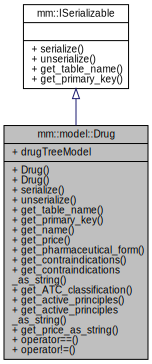
\includegraphics[width=224pt]{d1/d98/classmm_1_1model_1_1_drug__inherit__graph}
\end{center}
\end{figure}


Diagramma di collaborazione per mm\+:\+:model\+:\+:Drug\+:\nopagebreak
\begin{figure}[H]
\begin{center}
\leavevmode
\includegraphics[height=550pt]{d7/d98/classmm_1_1model_1_1_drug__coll__graph}
\end{center}
\end{figure}
\subsection*{Composti}
\begin{DoxyCompactItemize}
\item 
struct \hyperlink{structmm_1_1model_1_1_drug_1_1_tree_model}{Tree\+Model}
\end{DoxyCompactItemize}
\subsection*{Membri pubblici}
\begin{DoxyCompactItemize}
\item 
\hyperlink{classmm_1_1model_1_1_drug_a23f6e0538f52bd77fb8fa511392889a6}{Drug} (const string \&name, float price)
\item 
\hyperlink{classmm_1_1model_1_1_drug_a60cb5ecb3ed21da2f7f7e8bc94a1019d}{Drug} ()=default
\item 
map$<$ string, \hyperlink{structmm_1_1_serialized}{Serialized} $>$ \hyperlink{classmm_1_1model_1_1_drug_a5d4fa5bf5e4700f833547c5114764c7b}{serialize} () const override
\item 
void \hyperlink{classmm_1_1model_1_1_drug_adc9cd19eb2d0c3c271c01c41cf10d600}{unserialize} (map$<$ string, \hyperlink{structmm_1_1_serialized}{Serialized} $>$ map) override
\item 
string \hyperlink{classmm_1_1model_1_1_drug_a7fa9dbb569b89f397d4b865b778b3751}{get\+\_\+table\+\_\+name} () const override
\item 
vector$<$ string $>$ \hyperlink{classmm_1_1model_1_1_drug_a019770ab95f95f34bbc204c4c3860bfa}{get\+\_\+primary\+\_\+key} () const override
\item 
const string \& \hyperlink{classmm_1_1model_1_1_drug_ac01bfb91a074b57a3ba3b5b6f567e726}{get\+\_\+name} () const
\item 
float \hyperlink{classmm_1_1model_1_1_drug_a0add6ee0680f5028d0e820033ebada20}{get\+\_\+price} () const
\item 
const string \& \hyperlink{classmm_1_1model_1_1_drug_a2435614b64f13687d25b04f7d9335c9a}{get\+\_\+pharmaceutical\+\_\+form} () const
\item 
const vector$<$ string $>$ \& \hyperlink{classmm_1_1model_1_1_drug_a9116e111f2a546dbc35fd5e08863f37a}{get\+\_\+contraindications} () const
\item 
const string \hyperlink{classmm_1_1model_1_1_drug_a71f9f7d210a2fd7fbad86e61affd9105}{get\+\_\+contraindications\+\_\+as\+\_\+string} () const
\item 
const string \hyperlink{classmm_1_1model_1_1_drug_a64a1e99b4702d83b9c94379d14b4873b}{get\+\_\+\+A\+T\+C\+\_\+classification} () const
\item 
const vector$<$ pair$<$ string, string $>$ $>$ \& \hyperlink{classmm_1_1model_1_1_drug_a809666171510a2511573fa65d4dcd7cb}{get\+\_\+active\+\_\+principles} () const
\item 
const string \hyperlink{classmm_1_1model_1_1_drug_aaa9a406540607aed5845bb6af20b1231}{get\+\_\+active\+\_\+principles\+\_\+as\+\_\+string} () const
\item 
const string \hyperlink{classmm_1_1model_1_1_drug_ab5bfd8748a32b0cb366c4bf29633f00a}{get\+\_\+price\+\_\+as\+\_\+string} () const
\item 
bool \hyperlink{classmm_1_1model_1_1_drug_a15151e60eef91b544c63d8ff55db7bab}{operator==} (const \hyperlink{classmm_1_1model_1_1_drug}{Drug} \&rhs) const
\item 
bool \hyperlink{classmm_1_1model_1_1_drug_a51d9c5692835cab9d206580ccf8d0e1e}{operator!=} (const \hyperlink{classmm_1_1model_1_1_drug}{Drug} \&rhs) const
\end{DoxyCompactItemize}
\subsection*{Attributi pubblici statici}
\begin{DoxyCompactItemize}
\item 
static \hyperlink{structmm_1_1model_1_1_drug_1_1_tree_model}{Tree\+Model} \hyperlink{classmm_1_1model_1_1_drug_a9169612d0fc3b3b25063a1686be30af9}{drug\+Tree\+Model}
\end{DoxyCompactItemize}


\subsection{Documentazione dei costruttori e dei distruttori}
\mbox{\Hypertarget{classmm_1_1model_1_1_drug_a23f6e0538f52bd77fb8fa511392889a6}\label{classmm_1_1model_1_1_drug_a23f6e0538f52bd77fb8fa511392889a6}} 
\index{mm\+::model\+::\+Drug@{mm\+::model\+::\+Drug}!Drug@{Drug}}
\index{Drug@{Drug}!mm\+::model\+::\+Drug@{mm\+::model\+::\+Drug}}
\subsubsection{\texorpdfstring{Drug()}{Drug()}\hspace{0.1cm}{\footnotesize\ttfamily [1/2]}}
{\footnotesize\ttfamily mm\+::model\+::\+Drug\+::\+Drug (\begin{DoxyParamCaption}\item[{const string \&}]{name,  }\item[{float}]{price }\end{DoxyParamCaption})}

\mbox{\Hypertarget{classmm_1_1model_1_1_drug_a60cb5ecb3ed21da2f7f7e8bc94a1019d}\label{classmm_1_1model_1_1_drug_a60cb5ecb3ed21da2f7f7e8bc94a1019d}} 
\index{mm\+::model\+::\+Drug@{mm\+::model\+::\+Drug}!Drug@{Drug}}
\index{Drug@{Drug}!mm\+::model\+::\+Drug@{mm\+::model\+::\+Drug}}
\subsubsection{\texorpdfstring{Drug()}{Drug()}\hspace{0.1cm}{\footnotesize\ttfamily [2/2]}}
{\footnotesize\ttfamily mm\+::model\+::\+Drug\+::\+Drug (\begin{DoxyParamCaption}{ }\end{DoxyParamCaption})\hspace{0.3cm}{\ttfamily [default]}}



\subsection{Documentazione delle funzioni membro}
\mbox{\Hypertarget{classmm_1_1model_1_1_drug_a809666171510a2511573fa65d4dcd7cb}\label{classmm_1_1model_1_1_drug_a809666171510a2511573fa65d4dcd7cb}} 
\index{mm\+::model\+::\+Drug@{mm\+::model\+::\+Drug}!get\+\_\+active\+\_\+principles@{get\+\_\+active\+\_\+principles}}
\index{get\+\_\+active\+\_\+principles@{get\+\_\+active\+\_\+principles}!mm\+::model\+::\+Drug@{mm\+::model\+::\+Drug}}
\subsubsection{\texorpdfstring{get\+\_\+active\+\_\+principles()}{get\_active\_principles()}}
{\footnotesize\ttfamily const vector$<$ pair$<$ string, string $>$ $>$ \& mm\+::model\+::\+Drug\+::get\+\_\+active\+\_\+principles (\begin{DoxyParamCaption}{ }\end{DoxyParamCaption}) const}

\mbox{\Hypertarget{classmm_1_1model_1_1_drug_aaa9a406540607aed5845bb6af20b1231}\label{classmm_1_1model_1_1_drug_aaa9a406540607aed5845bb6af20b1231}} 
\index{mm\+::model\+::\+Drug@{mm\+::model\+::\+Drug}!get\+\_\+active\+\_\+principles\+\_\+as\+\_\+string@{get\+\_\+active\+\_\+principles\+\_\+as\+\_\+string}}
\index{get\+\_\+active\+\_\+principles\+\_\+as\+\_\+string@{get\+\_\+active\+\_\+principles\+\_\+as\+\_\+string}!mm\+::model\+::\+Drug@{mm\+::model\+::\+Drug}}
\subsubsection{\texorpdfstring{get\+\_\+active\+\_\+principles\+\_\+as\+\_\+string()}{get\_active\_principles\_as\_string()}}
{\footnotesize\ttfamily const string mm\+::model\+::\+Drug\+::get\+\_\+active\+\_\+principles\+\_\+as\+\_\+string (\begin{DoxyParamCaption}{ }\end{DoxyParamCaption}) const}

\mbox{\Hypertarget{classmm_1_1model_1_1_drug_a64a1e99b4702d83b9c94379d14b4873b}\label{classmm_1_1model_1_1_drug_a64a1e99b4702d83b9c94379d14b4873b}} 
\index{mm\+::model\+::\+Drug@{mm\+::model\+::\+Drug}!get\+\_\+\+A\+T\+C\+\_\+classification@{get\+\_\+\+A\+T\+C\+\_\+classification}}
\index{get\+\_\+\+A\+T\+C\+\_\+classification@{get\+\_\+\+A\+T\+C\+\_\+classification}!mm\+::model\+::\+Drug@{mm\+::model\+::\+Drug}}
\subsubsection{\texorpdfstring{get\+\_\+\+A\+T\+C\+\_\+classification()}{get\_ATC\_classification()}}
{\footnotesize\ttfamily const string mm\+::model\+::\+Drug\+::get\+\_\+\+A\+T\+C\+\_\+classification (\begin{DoxyParamCaption}{ }\end{DoxyParamCaption}) const}

\mbox{\Hypertarget{classmm_1_1model_1_1_drug_a9116e111f2a546dbc35fd5e08863f37a}\label{classmm_1_1model_1_1_drug_a9116e111f2a546dbc35fd5e08863f37a}} 
\index{mm\+::model\+::\+Drug@{mm\+::model\+::\+Drug}!get\+\_\+contraindications@{get\+\_\+contraindications}}
\index{get\+\_\+contraindications@{get\+\_\+contraindications}!mm\+::model\+::\+Drug@{mm\+::model\+::\+Drug}}
\subsubsection{\texorpdfstring{get\+\_\+contraindications()}{get\_contraindications()}}
{\footnotesize\ttfamily const vector$<$ string $>$ \& mm\+::model\+::\+Drug\+::get\+\_\+contraindications (\begin{DoxyParamCaption}{ }\end{DoxyParamCaption}) const}

\mbox{\Hypertarget{classmm_1_1model_1_1_drug_a71f9f7d210a2fd7fbad86e61affd9105}\label{classmm_1_1model_1_1_drug_a71f9f7d210a2fd7fbad86e61affd9105}} 
\index{mm\+::model\+::\+Drug@{mm\+::model\+::\+Drug}!get\+\_\+contraindications\+\_\+as\+\_\+string@{get\+\_\+contraindications\+\_\+as\+\_\+string}}
\index{get\+\_\+contraindications\+\_\+as\+\_\+string@{get\+\_\+contraindications\+\_\+as\+\_\+string}!mm\+::model\+::\+Drug@{mm\+::model\+::\+Drug}}
\subsubsection{\texorpdfstring{get\+\_\+contraindications\+\_\+as\+\_\+string()}{get\_contraindications\_as\_string()}}
{\footnotesize\ttfamily const string mm\+::model\+::\+Drug\+::get\+\_\+contraindications\+\_\+as\+\_\+string (\begin{DoxyParamCaption}{ }\end{DoxyParamCaption}) const}

\mbox{\Hypertarget{classmm_1_1model_1_1_drug_ac01bfb91a074b57a3ba3b5b6f567e726}\label{classmm_1_1model_1_1_drug_ac01bfb91a074b57a3ba3b5b6f567e726}} 
\index{mm\+::model\+::\+Drug@{mm\+::model\+::\+Drug}!get\+\_\+name@{get\+\_\+name}}
\index{get\+\_\+name@{get\+\_\+name}!mm\+::model\+::\+Drug@{mm\+::model\+::\+Drug}}
\subsubsection{\texorpdfstring{get\+\_\+name()}{get\_name()}}
{\footnotesize\ttfamily const string \& mm\+::model\+::\+Drug\+::get\+\_\+name (\begin{DoxyParamCaption}{ }\end{DoxyParamCaption}) const}

\mbox{\Hypertarget{classmm_1_1model_1_1_drug_a2435614b64f13687d25b04f7d9335c9a}\label{classmm_1_1model_1_1_drug_a2435614b64f13687d25b04f7d9335c9a}} 
\index{mm\+::model\+::\+Drug@{mm\+::model\+::\+Drug}!get\+\_\+pharmaceutical\+\_\+form@{get\+\_\+pharmaceutical\+\_\+form}}
\index{get\+\_\+pharmaceutical\+\_\+form@{get\+\_\+pharmaceutical\+\_\+form}!mm\+::model\+::\+Drug@{mm\+::model\+::\+Drug}}
\subsubsection{\texorpdfstring{get\+\_\+pharmaceutical\+\_\+form()}{get\_pharmaceutical\_form()}}
{\footnotesize\ttfamily const string \& mm\+::model\+::\+Drug\+::get\+\_\+pharmaceutical\+\_\+form (\begin{DoxyParamCaption}{ }\end{DoxyParamCaption}) const}

\mbox{\Hypertarget{classmm_1_1model_1_1_drug_a0add6ee0680f5028d0e820033ebada20}\label{classmm_1_1model_1_1_drug_a0add6ee0680f5028d0e820033ebada20}} 
\index{mm\+::model\+::\+Drug@{mm\+::model\+::\+Drug}!get\+\_\+price@{get\+\_\+price}}
\index{get\+\_\+price@{get\+\_\+price}!mm\+::model\+::\+Drug@{mm\+::model\+::\+Drug}}
\subsubsection{\texorpdfstring{get\+\_\+price()}{get\_price()}}
{\footnotesize\ttfamily float mm\+::model\+::\+Drug\+::get\+\_\+price (\begin{DoxyParamCaption}{ }\end{DoxyParamCaption}) const}

\mbox{\Hypertarget{classmm_1_1model_1_1_drug_ab5bfd8748a32b0cb366c4bf29633f00a}\label{classmm_1_1model_1_1_drug_ab5bfd8748a32b0cb366c4bf29633f00a}} 
\index{mm\+::model\+::\+Drug@{mm\+::model\+::\+Drug}!get\+\_\+price\+\_\+as\+\_\+string@{get\+\_\+price\+\_\+as\+\_\+string}}
\index{get\+\_\+price\+\_\+as\+\_\+string@{get\+\_\+price\+\_\+as\+\_\+string}!mm\+::model\+::\+Drug@{mm\+::model\+::\+Drug}}
\subsubsection{\texorpdfstring{get\+\_\+price\+\_\+as\+\_\+string()}{get\_price\_as\_string()}}
{\footnotesize\ttfamily const string mm\+::model\+::\+Drug\+::get\+\_\+price\+\_\+as\+\_\+string (\begin{DoxyParamCaption}{ }\end{DoxyParamCaption}) const}

\mbox{\Hypertarget{classmm_1_1model_1_1_drug_a019770ab95f95f34bbc204c4c3860bfa}\label{classmm_1_1model_1_1_drug_a019770ab95f95f34bbc204c4c3860bfa}} 
\index{mm\+::model\+::\+Drug@{mm\+::model\+::\+Drug}!get\+\_\+primary\+\_\+key@{get\+\_\+primary\+\_\+key}}
\index{get\+\_\+primary\+\_\+key@{get\+\_\+primary\+\_\+key}!mm\+::model\+::\+Drug@{mm\+::model\+::\+Drug}}
\subsubsection{\texorpdfstring{get\+\_\+primary\+\_\+key()}{get\_primary\_key()}}
{\footnotesize\ttfamily vector$<$ string $>$ mm\+::model\+::\+Drug\+::get\+\_\+primary\+\_\+key (\begin{DoxyParamCaption}{ }\end{DoxyParamCaption}) const\hspace{0.3cm}{\ttfamily [override]}, {\ttfamily [virtual]}}



Implementa \hyperlink{classmm_1_1_i_serializable_a69c0c514e11e386b6cb1fbd03f14da17}{mm\+::\+I\+Serializable}.

\mbox{\Hypertarget{classmm_1_1model_1_1_drug_a7fa9dbb569b89f397d4b865b778b3751}\label{classmm_1_1model_1_1_drug_a7fa9dbb569b89f397d4b865b778b3751}} 
\index{mm\+::model\+::\+Drug@{mm\+::model\+::\+Drug}!get\+\_\+table\+\_\+name@{get\+\_\+table\+\_\+name}}
\index{get\+\_\+table\+\_\+name@{get\+\_\+table\+\_\+name}!mm\+::model\+::\+Drug@{mm\+::model\+::\+Drug}}
\subsubsection{\texorpdfstring{get\+\_\+table\+\_\+name()}{get\_table\_name()}}
{\footnotesize\ttfamily string mm\+::model\+::\+Drug\+::get\+\_\+table\+\_\+name (\begin{DoxyParamCaption}{ }\end{DoxyParamCaption}) const\hspace{0.3cm}{\ttfamily [override]}, {\ttfamily [virtual]}}



Implementa \hyperlink{classmm_1_1_i_serializable_a9717e6da47fcbac3ffa2e68152464e0a}{mm\+::\+I\+Serializable}.

\mbox{\Hypertarget{classmm_1_1model_1_1_drug_a51d9c5692835cab9d206580ccf8d0e1e}\label{classmm_1_1model_1_1_drug_a51d9c5692835cab9d206580ccf8d0e1e}} 
\index{mm\+::model\+::\+Drug@{mm\+::model\+::\+Drug}!operator"!=@{operator"!=}}
\index{operator"!=@{operator"!=}!mm\+::model\+::\+Drug@{mm\+::model\+::\+Drug}}
\subsubsection{\texorpdfstring{operator"!=()}{operator!=()}}
{\footnotesize\ttfamily bool mm\+::model\+::\+Drug\+::operator!= (\begin{DoxyParamCaption}\item[{const \hyperlink{classmm_1_1model_1_1_drug}{Drug} \&}]{rhs }\end{DoxyParamCaption}) const}

\mbox{\Hypertarget{classmm_1_1model_1_1_drug_a15151e60eef91b544c63d8ff55db7bab}\label{classmm_1_1model_1_1_drug_a15151e60eef91b544c63d8ff55db7bab}} 
\index{mm\+::model\+::\+Drug@{mm\+::model\+::\+Drug}!operator==@{operator==}}
\index{operator==@{operator==}!mm\+::model\+::\+Drug@{mm\+::model\+::\+Drug}}
\subsubsection{\texorpdfstring{operator==()}{operator==()}}
{\footnotesize\ttfamily bool mm\+::model\+::\+Drug\+::operator== (\begin{DoxyParamCaption}\item[{const \hyperlink{classmm_1_1model_1_1_drug}{Drug} \&}]{rhs }\end{DoxyParamCaption}) const}

\mbox{\Hypertarget{classmm_1_1model_1_1_drug_a5d4fa5bf5e4700f833547c5114764c7b}\label{classmm_1_1model_1_1_drug_a5d4fa5bf5e4700f833547c5114764c7b}} 
\index{mm\+::model\+::\+Drug@{mm\+::model\+::\+Drug}!serialize@{serialize}}
\index{serialize@{serialize}!mm\+::model\+::\+Drug@{mm\+::model\+::\+Drug}}
\subsubsection{\texorpdfstring{serialize()}{serialize()}}
{\footnotesize\ttfamily map$<$ string, \hyperlink{structmm_1_1_serialized}{mm\+::\+Serialized} $>$ mm\+::model\+::\+Drug\+::serialize (\begin{DoxyParamCaption}{ }\end{DoxyParamCaption}) const\hspace{0.3cm}{\ttfamily [override]}, {\ttfamily [virtual]}}



Implementa \hyperlink{classmm_1_1_i_serializable_a20a59e2324c8dbf6fefe4d11ae89d0fb}{mm\+::\+I\+Serializable}.

\mbox{\Hypertarget{classmm_1_1model_1_1_drug_adc9cd19eb2d0c3c271c01c41cf10d600}\label{classmm_1_1model_1_1_drug_adc9cd19eb2d0c3c271c01c41cf10d600}} 
\index{mm\+::model\+::\+Drug@{mm\+::model\+::\+Drug}!unserialize@{unserialize}}
\index{unserialize@{unserialize}!mm\+::model\+::\+Drug@{mm\+::model\+::\+Drug}}
\subsubsection{\texorpdfstring{unserialize()}{unserialize()}}
{\footnotesize\ttfamily void mm\+::model\+::\+Drug\+::unserialize (\begin{DoxyParamCaption}\item[{map$<$ string, \hyperlink{structmm_1_1_serialized}{Serialized} $>$}]{map }\end{DoxyParamCaption})\hspace{0.3cm}{\ttfamily [override]}}



\subsection{Documentazione dei membri dato}
\mbox{\Hypertarget{classmm_1_1model_1_1_drug_a9169612d0fc3b3b25063a1686be30af9}\label{classmm_1_1model_1_1_drug_a9169612d0fc3b3b25063a1686be30af9}} 
\index{mm\+::model\+::\+Drug@{mm\+::model\+::\+Drug}!drug\+Tree\+Model@{drug\+Tree\+Model}}
\index{drug\+Tree\+Model@{drug\+Tree\+Model}!mm\+::model\+::\+Drug@{mm\+::model\+::\+Drug}}
\subsubsection{\texorpdfstring{drug\+Tree\+Model}{drugTreeModel}}
{\footnotesize\ttfamily \hyperlink{structmm_1_1model_1_1_drug_1_1_tree_model}{mm\+::model\+::\+Drug\+::\+Tree\+Model} mm\+::model\+::\+Drug\+::drug\+Tree\+Model\hspace{0.3cm}{\ttfamily [static]}}

Project Elaborato\+\_\+\+I\+N\+G\+\_\+\+SW \begin{DoxyAuthor}{Autore}
Noè Murr, Mirko Morati 
\end{DoxyAuthor}


La documentazione per questa classe è stata generata a partire dai seguenti file\+:\begin{DoxyCompactItemize}
\item 
code/model/\hyperlink{_drug_8hpp}{Drug.\+hpp}\item 
code/model/\hyperlink{_drug_8cpp}{Drug.\+cpp}\end{DoxyCompactItemize}

\hypertarget{classmm_1_1view_1_1_drug_entry}{}\section{Riferimenti per la classe mm\+:\+:view\+:\+:Drug\+Entry}
\label{classmm_1_1view_1_1_drug_entry}\index{mm\+::view\+::\+Drug\+Entry@{mm\+::view\+::\+Drug\+Entry}}


{\ttfamily \#include $<$Custom\+Widgets.\+hpp$>$}



Diagramma delle classi per mm\+:\+:view\+:\+:Drug\+Entry
\nopagebreak
\begin{figure}[H]
\begin{center}
\leavevmode
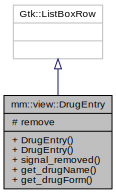
\includegraphics[width=189pt]{d6/d98/classmm_1_1view_1_1_drug_entry__inherit__graph}
\end{center}
\end{figure}


Diagramma di collaborazione per mm\+:\+:view\+:\+:Drug\+Entry\+:
\nopagebreak
\begin{figure}[H]
\begin{center}
\leavevmode
\includegraphics[width=189pt]{d7/dc4/classmm_1_1view_1_1_drug_entry__coll__graph}
\end{center}
\end{figure}
\subsection*{Membri pubblici}
\begin{DoxyCompactItemize}
\item 
\mbox{\hyperlink{classmm_1_1view_1_1_drug_entry_a7ad0e954cd9933565be5a86d6a808249}{Drug\+Entry}} ()=delete
\item 
\mbox{\hyperlink{classmm_1_1view_1_1_drug_entry_ac1fceaa91adf2812b93c1e1388068c27}{Drug\+Entry}} (const Glib\+::ustring \&drug)
\item 
sigc\+::signal$<$ void, \mbox{\hyperlink{classmm_1_1view_1_1_drug_entry}{mm\+::view\+::\+Drug\+Entry}} $\ast$ $>$ \mbox{\hyperlink{classmm_1_1view_1_1_drug_entry_aa7a9f1fd2d7a48a803314fa2c9a86370}{signal\+\_\+removed}} ()
\item 
const string \mbox{\hyperlink{classmm_1_1view_1_1_drug_entry_ada43ec12abdaf70f4c3070b6e7f9806d}{get\+\_\+drug\+Name}} () const
\item 
const string \mbox{\hyperlink{classmm_1_1view_1_1_drug_entry_a9034293f6c4dbe85af9d02751684d845}{get\+\_\+drug\+Form}} () const
\end{DoxyCompactItemize}
\subsection*{Attributi protetti}
\begin{DoxyCompactItemize}
\item 
sigc\+::signal$<$ void, \mbox{\hyperlink{classmm_1_1view_1_1_drug_entry}{mm\+::view\+::\+Drug\+Entry}} $\ast$ $>$ \mbox{\hyperlink{classmm_1_1view_1_1_drug_entry_a34bee6e0f8a4722c4e41b333eac49f60}{remove}}
\end{DoxyCompactItemize}


\subsection{Documentazione dei costruttori e dei distruttori}
\mbox{\Hypertarget{classmm_1_1view_1_1_drug_entry_a7ad0e954cd9933565be5a86d6a808249}\label{classmm_1_1view_1_1_drug_entry_a7ad0e954cd9933565be5a86d6a808249}} 
\index{mm\+::view\+::\+Drug\+Entry@{mm\+::view\+::\+Drug\+Entry}!Drug\+Entry@{Drug\+Entry}}
\index{Drug\+Entry@{Drug\+Entry}!mm\+::view\+::\+Drug\+Entry@{mm\+::view\+::\+Drug\+Entry}}
\subsubsection{\texorpdfstring{Drug\+Entry()}{DrugEntry()}\hspace{0.1cm}{\footnotesize\ttfamily [1/2]}}
{\footnotesize\ttfamily mm\+::view\+::\+Drug\+Entry\+::\+Drug\+Entry (\begin{DoxyParamCaption}{ }\end{DoxyParamCaption})\hspace{0.3cm}{\ttfamily [delete]}}

\mbox{\Hypertarget{classmm_1_1view_1_1_drug_entry_ac1fceaa91adf2812b93c1e1388068c27}\label{classmm_1_1view_1_1_drug_entry_ac1fceaa91adf2812b93c1e1388068c27}} 
\index{mm\+::view\+::\+Drug\+Entry@{mm\+::view\+::\+Drug\+Entry}!Drug\+Entry@{Drug\+Entry}}
\index{Drug\+Entry@{Drug\+Entry}!mm\+::view\+::\+Drug\+Entry@{mm\+::view\+::\+Drug\+Entry}}
\subsubsection{\texorpdfstring{Drug\+Entry()}{DrugEntry()}\hspace{0.1cm}{\footnotesize\ttfamily [2/2]}}
{\footnotesize\ttfamily mm\+::view\+::\+Drug\+Entry\+::\+Drug\+Entry (\begin{DoxyParamCaption}\item[{const Glib\+::ustring \&}]{drug }\end{DoxyParamCaption})}



\subsection{Documentazione delle funzioni membro}
\mbox{\Hypertarget{classmm_1_1view_1_1_drug_entry_a9034293f6c4dbe85af9d02751684d845}\label{classmm_1_1view_1_1_drug_entry_a9034293f6c4dbe85af9d02751684d845}} 
\index{mm\+::view\+::\+Drug\+Entry@{mm\+::view\+::\+Drug\+Entry}!get\+\_\+drug\+Form@{get\+\_\+drug\+Form}}
\index{get\+\_\+drug\+Form@{get\+\_\+drug\+Form}!mm\+::view\+::\+Drug\+Entry@{mm\+::view\+::\+Drug\+Entry}}
\subsubsection{\texorpdfstring{get\+\_\+drug\+Form()}{get\_drugForm()}}
{\footnotesize\ttfamily const string mm\+::view\+::\+Drug\+Entry\+::get\+\_\+drug\+Form (\begin{DoxyParamCaption}{ }\end{DoxyParamCaption}) const}

\mbox{\Hypertarget{classmm_1_1view_1_1_drug_entry_ada43ec12abdaf70f4c3070b6e7f9806d}\label{classmm_1_1view_1_1_drug_entry_ada43ec12abdaf70f4c3070b6e7f9806d}} 
\index{mm\+::view\+::\+Drug\+Entry@{mm\+::view\+::\+Drug\+Entry}!get\+\_\+drug\+Name@{get\+\_\+drug\+Name}}
\index{get\+\_\+drug\+Name@{get\+\_\+drug\+Name}!mm\+::view\+::\+Drug\+Entry@{mm\+::view\+::\+Drug\+Entry}}
\subsubsection{\texorpdfstring{get\+\_\+drug\+Name()}{get\_drugName()}}
{\footnotesize\ttfamily const string mm\+::view\+::\+Drug\+Entry\+::get\+\_\+drug\+Name (\begin{DoxyParamCaption}{ }\end{DoxyParamCaption}) const}

\mbox{\Hypertarget{classmm_1_1view_1_1_drug_entry_aa7a9f1fd2d7a48a803314fa2c9a86370}\label{classmm_1_1view_1_1_drug_entry_aa7a9f1fd2d7a48a803314fa2c9a86370}} 
\index{mm\+::view\+::\+Drug\+Entry@{mm\+::view\+::\+Drug\+Entry}!signal\+\_\+removed@{signal\+\_\+removed}}
\index{signal\+\_\+removed@{signal\+\_\+removed}!mm\+::view\+::\+Drug\+Entry@{mm\+::view\+::\+Drug\+Entry}}
\subsubsection{\texorpdfstring{signal\+\_\+removed()}{signal\_removed()}}
{\footnotesize\ttfamily sigc\+::signal$<$ void, \mbox{\hyperlink{classmm_1_1view_1_1_drug_entry}{mm\+::view\+::\+Drug\+Entry}} $\ast$ $>$ mm\+::view\+::\+Drug\+Entry\+::signal\+\_\+removed (\begin{DoxyParamCaption}{ }\end{DoxyParamCaption})}



\subsection{Documentazione dei membri dato}
\mbox{\Hypertarget{classmm_1_1view_1_1_drug_entry_a34bee6e0f8a4722c4e41b333eac49f60}\label{classmm_1_1view_1_1_drug_entry_a34bee6e0f8a4722c4e41b333eac49f60}} 
\index{mm\+::view\+::\+Drug\+Entry@{mm\+::view\+::\+Drug\+Entry}!remove@{remove}}
\index{remove@{remove}!mm\+::view\+::\+Drug\+Entry@{mm\+::view\+::\+Drug\+Entry}}
\subsubsection{\texorpdfstring{remove}{remove}}
{\footnotesize\ttfamily sigc\+::signal$<$void, \mbox{\hyperlink{classmm_1_1view_1_1_drug_entry}{mm\+::view\+::\+Drug\+Entry}} $\ast$$>$ mm\+::view\+::\+Drug\+Entry\+::remove\hspace{0.3cm}{\ttfamily [protected]}}



La documentazione per questa classe è stata generata a partire dai seguenti file\+:\begin{DoxyCompactItemize}
\item 
code/gui/view/\mbox{\hyperlink{_custom_widgets_8hpp}{Custom\+Widgets.\+hpp}}\item 
code/gui/view/\mbox{\hyperlink{_custom_widgets_8cpp}{Custom\+Widgets.\+cpp}}\end{DoxyCompactItemize}

\hypertarget{structmm_1_1model_1_1_drug_tree_model}{}\section{Riferimenti per la struct mm\+:\+:model\+:\+:Drug\+Tree\+Model}
\label{structmm_1_1model_1_1_drug_tree_model}\index{mm\+::model\+::\+Drug\+Tree\+Model@{mm\+::model\+::\+Drug\+Tree\+Model}}


{\ttfamily \#include $<$Drug.\+hpp$>$}



Diagramma delle classi per mm\+:\+:model\+:\+:Drug\+Tree\+Model
\nopagebreak
\begin{figure}[H]
\begin{center}
\leavevmode
\includegraphics[width=237pt]{d8/d2a/structmm_1_1model_1_1_drug_tree_model__inherit__graph}
\end{center}
\end{figure}


Diagramma di collaborazione per mm\+:\+:model\+:\+:Drug\+Tree\+Model\+:
\nopagebreak
\begin{figure}[H]
\begin{center}
\leavevmode
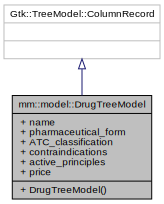
\includegraphics[width=237pt]{dd/d75/structmm_1_1model_1_1_drug_tree_model__coll__graph}
\end{center}
\end{figure}
\subsection*{Membri pubblici}
\begin{DoxyCompactItemize}
\item 
\mbox{\hyperlink{structmm_1_1model_1_1_drug_tree_model_a4fe945eeb529bbd8d3f19aa7797764d9}{Drug\+Tree\+Model}} ()
\end{DoxyCompactItemize}
\subsection*{Attributi pubblici}
\begin{DoxyCompactItemize}
\item 
Gtk\+::\+Tree\+Model\+Column$<$ Glib\+::ustring $>$ \mbox{\hyperlink{structmm_1_1model_1_1_drug_tree_model_aae1c93a96cd321861445996965814405}{name}}
\item 
Gtk\+::\+Tree\+Model\+Column$<$ Glib\+::ustring $>$ \mbox{\hyperlink{structmm_1_1model_1_1_drug_tree_model_aa93ee13951feb310e5b31775ebf74609}{pharmaceutical\+\_\+form}}
\item 
Gtk\+::\+Tree\+Model\+Column$<$ Glib\+::ustring $>$ \mbox{\hyperlink{structmm_1_1model_1_1_drug_tree_model_a0462c8a43912e7d9b24d302899c73ddd}{A\+T\+C\+\_\+classification}}
\item 
Gtk\+::\+Tree\+Model\+Column$<$ Glib\+::ustring $>$ \mbox{\hyperlink{structmm_1_1model_1_1_drug_tree_model_a6c23e14f0c72622e29de9a8d2534dbdd}{contraindications}}
\item 
Gtk\+::\+Tree\+Model\+Column$<$ Glib\+::ustring $>$ \mbox{\hyperlink{structmm_1_1model_1_1_drug_tree_model_aa4e0565da99c9e2e41dc8ed416c66903}{active\+\_\+principles}}
\item 
Gtk\+::\+Tree\+Model\+Column$<$ Glib\+::ustring $>$ \mbox{\hyperlink{structmm_1_1model_1_1_drug_tree_model_a19f5c8676ecd88d4bb8b6f5d161d8a6b}{price}}
\end{DoxyCompactItemize}


\subsection{Documentazione dei costruttori e dei distruttori}
\mbox{\Hypertarget{structmm_1_1model_1_1_drug_tree_model_a4fe945eeb529bbd8d3f19aa7797764d9}\label{structmm_1_1model_1_1_drug_tree_model_a4fe945eeb529bbd8d3f19aa7797764d9}} 
\index{mm\+::model\+::\+Drug\+Tree\+Model@{mm\+::model\+::\+Drug\+Tree\+Model}!Drug\+Tree\+Model@{Drug\+Tree\+Model}}
\index{Drug\+Tree\+Model@{Drug\+Tree\+Model}!mm\+::model\+::\+Drug\+Tree\+Model@{mm\+::model\+::\+Drug\+Tree\+Model}}
\subsubsection{\texorpdfstring{Drug\+Tree\+Model()}{DrugTreeModel()}}
{\footnotesize\ttfamily mm\+::model\+::\+Drug\+Tree\+Model\+::\+Drug\+Tree\+Model (\begin{DoxyParamCaption}{ }\end{DoxyParamCaption})\hspace{0.3cm}{\ttfamily [inline]}}



\subsection{Documentazione dei membri dato}
\mbox{\Hypertarget{structmm_1_1model_1_1_drug_tree_model_aa4e0565da99c9e2e41dc8ed416c66903}\label{structmm_1_1model_1_1_drug_tree_model_aa4e0565da99c9e2e41dc8ed416c66903}} 
\index{mm\+::model\+::\+Drug\+Tree\+Model@{mm\+::model\+::\+Drug\+Tree\+Model}!active\+\_\+principles@{active\+\_\+principles}}
\index{active\+\_\+principles@{active\+\_\+principles}!mm\+::model\+::\+Drug\+Tree\+Model@{mm\+::model\+::\+Drug\+Tree\+Model}}
\subsubsection{\texorpdfstring{active\+\_\+principles}{active\_principles}}
{\footnotesize\ttfamily Gtk\+::\+Tree\+Model\+Column$<$Glib\+::ustring$>$ mm\+::model\+::\+Drug\+Tree\+Model\+::active\+\_\+principles}

\mbox{\Hypertarget{structmm_1_1model_1_1_drug_tree_model_a0462c8a43912e7d9b24d302899c73ddd}\label{structmm_1_1model_1_1_drug_tree_model_a0462c8a43912e7d9b24d302899c73ddd}} 
\index{mm\+::model\+::\+Drug\+Tree\+Model@{mm\+::model\+::\+Drug\+Tree\+Model}!A\+T\+C\+\_\+classification@{A\+T\+C\+\_\+classification}}
\index{A\+T\+C\+\_\+classification@{A\+T\+C\+\_\+classification}!mm\+::model\+::\+Drug\+Tree\+Model@{mm\+::model\+::\+Drug\+Tree\+Model}}
\subsubsection{\texorpdfstring{A\+T\+C\+\_\+classification}{ATC\_classification}}
{\footnotesize\ttfamily Gtk\+::\+Tree\+Model\+Column$<$Glib\+::ustring$>$ mm\+::model\+::\+Drug\+Tree\+Model\+::\+A\+T\+C\+\_\+classification}

\mbox{\Hypertarget{structmm_1_1model_1_1_drug_tree_model_a6c23e14f0c72622e29de9a8d2534dbdd}\label{structmm_1_1model_1_1_drug_tree_model_a6c23e14f0c72622e29de9a8d2534dbdd}} 
\index{mm\+::model\+::\+Drug\+Tree\+Model@{mm\+::model\+::\+Drug\+Tree\+Model}!contraindications@{contraindications}}
\index{contraindications@{contraindications}!mm\+::model\+::\+Drug\+Tree\+Model@{mm\+::model\+::\+Drug\+Tree\+Model}}
\subsubsection{\texorpdfstring{contraindications}{contraindications}}
{\footnotesize\ttfamily Gtk\+::\+Tree\+Model\+Column$<$Glib\+::ustring$>$ mm\+::model\+::\+Drug\+Tree\+Model\+::contraindications}

\mbox{\Hypertarget{structmm_1_1model_1_1_drug_tree_model_aae1c93a96cd321861445996965814405}\label{structmm_1_1model_1_1_drug_tree_model_aae1c93a96cd321861445996965814405}} 
\index{mm\+::model\+::\+Drug\+Tree\+Model@{mm\+::model\+::\+Drug\+Tree\+Model}!name@{name}}
\index{name@{name}!mm\+::model\+::\+Drug\+Tree\+Model@{mm\+::model\+::\+Drug\+Tree\+Model}}
\subsubsection{\texorpdfstring{name}{name}}
{\footnotesize\ttfamily Gtk\+::\+Tree\+Model\+Column$<$Glib\+::ustring$>$ mm\+::model\+::\+Drug\+Tree\+Model\+::name}

\mbox{\Hypertarget{structmm_1_1model_1_1_drug_tree_model_aa93ee13951feb310e5b31775ebf74609}\label{structmm_1_1model_1_1_drug_tree_model_aa93ee13951feb310e5b31775ebf74609}} 
\index{mm\+::model\+::\+Drug\+Tree\+Model@{mm\+::model\+::\+Drug\+Tree\+Model}!pharmaceutical\+\_\+form@{pharmaceutical\+\_\+form}}
\index{pharmaceutical\+\_\+form@{pharmaceutical\+\_\+form}!mm\+::model\+::\+Drug\+Tree\+Model@{mm\+::model\+::\+Drug\+Tree\+Model}}
\subsubsection{\texorpdfstring{pharmaceutical\+\_\+form}{pharmaceutical\_form}}
{\footnotesize\ttfamily Gtk\+::\+Tree\+Model\+Column$<$Glib\+::ustring$>$ mm\+::model\+::\+Drug\+Tree\+Model\+::pharmaceutical\+\_\+form}

\mbox{\Hypertarget{structmm_1_1model_1_1_drug_tree_model_a19f5c8676ecd88d4bb8b6f5d161d8a6b}\label{structmm_1_1model_1_1_drug_tree_model_a19f5c8676ecd88d4bb8b6f5d161d8a6b}} 
\index{mm\+::model\+::\+Drug\+Tree\+Model@{mm\+::model\+::\+Drug\+Tree\+Model}!price@{price}}
\index{price@{price}!mm\+::model\+::\+Drug\+Tree\+Model@{mm\+::model\+::\+Drug\+Tree\+Model}}
\subsubsection{\texorpdfstring{price}{price}}
{\footnotesize\ttfamily Gtk\+::\+Tree\+Model\+Column$<$Glib\+::ustring$>$ mm\+::model\+::\+Drug\+Tree\+Model\+::price}



La documentazione per questa struct è stata generata a partire dal seguente file\+:\begin{DoxyCompactItemize}
\item 
code/model/\mbox{\hyperlink{_drug_8hpp}{Drug.\+hpp}}\end{DoxyCompactItemize}

\hypertarget{classmm_1_1_drug_window}{}\section{Riferimenti per la classe mm\+:\+:Drug\+Window}
\label{classmm_1_1_drug_window}\index{mm\+::\+Drug\+Window@{mm\+::\+Drug\+Window}}


{\ttfamily \#include $<$Drug\+Window.\+hpp$>$}



Diagramma delle classi per mm\+:\+:Drug\+Window
\nopagebreak
\begin{figure}[H]
\begin{center}
\leavevmode
\includegraphics[width=309pt]{d6/d16/classmm_1_1_drug_window__inherit__graph}
\end{center}
\end{figure}


Diagramma di collaborazione per mm\+:\+:Drug\+Window\+:
\nopagebreak
\begin{figure}[H]
\begin{center}
\leavevmode
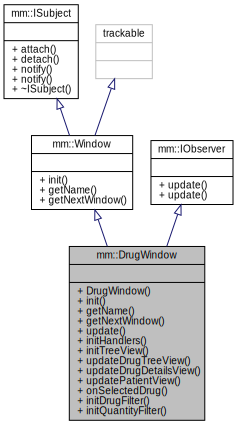
\includegraphics[width=309pt]{d8/d52/classmm_1_1_drug_window__coll__graph}
\end{center}
\end{figure}
\subsection*{Membri pubblici}
\begin{DoxyCompactItemize}
\item 
\mbox{\hyperlink{classmm_1_1_drug_window_a7324435f0124010f172507467454d1a5}{Drug\+Window}} ()
\item 
bool \mbox{\hyperlink{classmm_1_1_drug_window_a54f331f1c516ce9113a9dade43948a16}{init}} () override
\item 
\mbox{\hyperlink{namespacemm_a4e9d92e04f65dbf2fc1963947da0d93c}{Window\+Name}} \mbox{\hyperlink{classmm_1_1_drug_window_aa33aafc6205abc8c627d0b0a5849895b}{get\+Name}} () const override
\item 
\mbox{\hyperlink{namespacemm_a4e9d92e04f65dbf2fc1963947da0d93c}{Window\+Name}} \mbox{\hyperlink{classmm_1_1_drug_window_a571966bdd4a2ecf069cdca69c73726b2}{get\+Next\+Window}} () const override
\item 
void \mbox{\hyperlink{classmm_1_1_drug_window_a98c6d97f491cb648dede0ef3db2b13b2}{update}} () override
\item 
void \mbox{\hyperlink{classmm_1_1_drug_window_a4926180df1b7f3dfc1f2b1746522c6fb}{init\+Handlers}} ()
\item 
void \mbox{\hyperlink{classmm_1_1_drug_window_ac762c909bb394adccd41e1c6e97d8404}{init\+Tree\+View}} ()
\item 
void \mbox{\hyperlink{classmm_1_1_drug_window_a7a43f5981915470da37088a248006c0e}{update\+Drug\+Tree\+View}} ()
\item 
void \mbox{\hyperlink{classmm_1_1_drug_window_a5df5a3991bc26fcf5e4df2c622053c42}{update\+Drug\+Details\+View}} ()
\item 
void \mbox{\hyperlink{classmm_1_1_drug_window_a069d6731dcbf47f32e6be18a8ecb0472}{update\+Patient\+View}} ()
\item 
void \mbox{\hyperlink{classmm_1_1_drug_window_ad88417beac6e778776f939c31e6def7a}{on\+Selected\+Drug}} (const Gtk\+::\+Tree\+Model\+::\+Path \&, Gtk\+::\+Tree\+View\+Column $\ast$)
\item 
void \mbox{\hyperlink{classmm_1_1_drug_window_a2d01e24deaba42b7c24cf5b5457f4298}{init\+Drug\+Filter}} ()
\item 
void \mbox{\hyperlink{classmm_1_1_drug_window_a40c9dca8380e72b7468170db21bcfbe9}{init\+Quantity\+Filter}} ()
\end{DoxyCompactItemize}


\subsection{Documentazione dei costruttori e dei distruttori}
\mbox{\Hypertarget{classmm_1_1_drug_window_a7324435f0124010f172507467454d1a5}\label{classmm_1_1_drug_window_a7324435f0124010f172507467454d1a5}} 
\index{mm\+::\+Drug\+Window@{mm\+::\+Drug\+Window}!Drug\+Window@{Drug\+Window}}
\index{Drug\+Window@{Drug\+Window}!mm\+::\+Drug\+Window@{mm\+::\+Drug\+Window}}
\subsubsection{\texorpdfstring{Drug\+Window()}{DrugWindow()}}
{\footnotesize\ttfamily mm\+::\+Drug\+Window\+::\+Drug\+Window (\begin{DoxyParamCaption}{ }\end{DoxyParamCaption})}



\subsection{Documentazione delle funzioni membro}
\mbox{\Hypertarget{classmm_1_1_drug_window_aa33aafc6205abc8c627d0b0a5849895b}\label{classmm_1_1_drug_window_aa33aafc6205abc8c627d0b0a5849895b}} 
\index{mm\+::\+Drug\+Window@{mm\+::\+Drug\+Window}!get\+Name@{get\+Name}}
\index{get\+Name@{get\+Name}!mm\+::\+Drug\+Window@{mm\+::\+Drug\+Window}}
\subsubsection{\texorpdfstring{get\+Name()}{getName()}}
{\footnotesize\ttfamily \mbox{\hyperlink{namespacemm_a4e9d92e04f65dbf2fc1963947da0d93c}{mm\+::\+Window\+Name}} mm\+::\+Drug\+Window\+::get\+Name (\begin{DoxyParamCaption}{ }\end{DoxyParamCaption}) const\hspace{0.3cm}{\ttfamily [override]}, {\ttfamily [virtual]}}



Implementa \mbox{\hyperlink{classmm_1_1_window_a942c9125bf42156a9f7b7f561e412fed}{mm\+::\+Window}}.

\mbox{\Hypertarget{classmm_1_1_drug_window_a571966bdd4a2ecf069cdca69c73726b2}\label{classmm_1_1_drug_window_a571966bdd4a2ecf069cdca69c73726b2}} 
\index{mm\+::\+Drug\+Window@{mm\+::\+Drug\+Window}!get\+Next\+Window@{get\+Next\+Window}}
\index{get\+Next\+Window@{get\+Next\+Window}!mm\+::\+Drug\+Window@{mm\+::\+Drug\+Window}}
\subsubsection{\texorpdfstring{get\+Next\+Window()}{getNextWindow()}}
{\footnotesize\ttfamily \mbox{\hyperlink{namespacemm_a4e9d92e04f65dbf2fc1963947da0d93c}{mm\+::\+Window\+Name}} mm\+::\+Drug\+Window\+::get\+Next\+Window (\begin{DoxyParamCaption}{ }\end{DoxyParamCaption}) const\hspace{0.3cm}{\ttfamily [override]}, {\ttfamily [virtual]}}



Implementa \mbox{\hyperlink{classmm_1_1_window_a0cd7b4b0feb9505c44503547a161fcd8}{mm\+::\+Window}}.

\mbox{\Hypertarget{classmm_1_1_drug_window_a54f331f1c516ce9113a9dade43948a16}\label{classmm_1_1_drug_window_a54f331f1c516ce9113a9dade43948a16}} 
\index{mm\+::\+Drug\+Window@{mm\+::\+Drug\+Window}!init@{init}}
\index{init@{init}!mm\+::\+Drug\+Window@{mm\+::\+Drug\+Window}}
\subsubsection{\texorpdfstring{init()}{init()}}
{\footnotesize\ttfamily bool mm\+::\+Drug\+Window\+::init (\begin{DoxyParamCaption}{ }\end{DoxyParamCaption})\hspace{0.3cm}{\ttfamily [override]}, {\ttfamily [virtual]}}



Implementa \mbox{\hyperlink{classmm_1_1_window_aba03fbf4761b2f106352baecf5996e10}{mm\+::\+Window}}.

\mbox{\Hypertarget{classmm_1_1_drug_window_a2d01e24deaba42b7c24cf5b5457f4298}\label{classmm_1_1_drug_window_a2d01e24deaba42b7c24cf5b5457f4298}} 
\index{mm\+::\+Drug\+Window@{mm\+::\+Drug\+Window}!init\+Drug\+Filter@{init\+Drug\+Filter}}
\index{init\+Drug\+Filter@{init\+Drug\+Filter}!mm\+::\+Drug\+Window@{mm\+::\+Drug\+Window}}
\subsubsection{\texorpdfstring{init\+Drug\+Filter()}{initDrugFilter()}}
{\footnotesize\ttfamily void mm\+::\+Drug\+Window\+::init\+Drug\+Filter (\begin{DoxyParamCaption}{ }\end{DoxyParamCaption})}

\mbox{\Hypertarget{classmm_1_1_drug_window_a4926180df1b7f3dfc1f2b1746522c6fb}\label{classmm_1_1_drug_window_a4926180df1b7f3dfc1f2b1746522c6fb}} 
\index{mm\+::\+Drug\+Window@{mm\+::\+Drug\+Window}!init\+Handlers@{init\+Handlers}}
\index{init\+Handlers@{init\+Handlers}!mm\+::\+Drug\+Window@{mm\+::\+Drug\+Window}}
\subsubsection{\texorpdfstring{init\+Handlers()}{initHandlers()}}
{\footnotesize\ttfamily void mm\+::\+Drug\+Window\+::init\+Handlers (\begin{DoxyParamCaption}{ }\end{DoxyParamCaption})}

\mbox{\Hypertarget{classmm_1_1_drug_window_a40c9dca8380e72b7468170db21bcfbe9}\label{classmm_1_1_drug_window_a40c9dca8380e72b7468170db21bcfbe9}} 
\index{mm\+::\+Drug\+Window@{mm\+::\+Drug\+Window}!init\+Quantity\+Filter@{init\+Quantity\+Filter}}
\index{init\+Quantity\+Filter@{init\+Quantity\+Filter}!mm\+::\+Drug\+Window@{mm\+::\+Drug\+Window}}
\subsubsection{\texorpdfstring{init\+Quantity\+Filter()}{initQuantityFilter()}}
{\footnotesize\ttfamily void mm\+::\+Drug\+Window\+::init\+Quantity\+Filter (\begin{DoxyParamCaption}{ }\end{DoxyParamCaption})}

\mbox{\Hypertarget{classmm_1_1_drug_window_ac762c909bb394adccd41e1c6e97d8404}\label{classmm_1_1_drug_window_ac762c909bb394adccd41e1c6e97d8404}} 
\index{mm\+::\+Drug\+Window@{mm\+::\+Drug\+Window}!init\+Tree\+View@{init\+Tree\+View}}
\index{init\+Tree\+View@{init\+Tree\+View}!mm\+::\+Drug\+Window@{mm\+::\+Drug\+Window}}
\subsubsection{\texorpdfstring{init\+Tree\+View()}{initTreeView()}}
{\footnotesize\ttfamily void mm\+::\+Drug\+Window\+::init\+Tree\+View (\begin{DoxyParamCaption}{ }\end{DoxyParamCaption})}

\mbox{\Hypertarget{classmm_1_1_drug_window_ad88417beac6e778776f939c31e6def7a}\label{classmm_1_1_drug_window_ad88417beac6e778776f939c31e6def7a}} 
\index{mm\+::\+Drug\+Window@{mm\+::\+Drug\+Window}!on\+Selected\+Drug@{on\+Selected\+Drug}}
\index{on\+Selected\+Drug@{on\+Selected\+Drug}!mm\+::\+Drug\+Window@{mm\+::\+Drug\+Window}}
\subsubsection{\texorpdfstring{on\+Selected\+Drug()}{onSelectedDrug()}}
{\footnotesize\ttfamily void mm\+::\+Drug\+Window\+::on\+Selected\+Drug (\begin{DoxyParamCaption}\item[{const Gtk\+::\+Tree\+Model\+::\+Path \&}]{,  }\item[{Gtk\+::\+Tree\+View\+Column $\ast$}]{ }\end{DoxyParamCaption})}

\mbox{\Hypertarget{classmm_1_1_drug_window_a98c6d97f491cb648dede0ef3db2b13b2}\label{classmm_1_1_drug_window_a98c6d97f491cb648dede0ef3db2b13b2}} 
\index{mm\+::\+Drug\+Window@{mm\+::\+Drug\+Window}!update@{update}}
\index{update@{update}!mm\+::\+Drug\+Window@{mm\+::\+Drug\+Window}}
\subsubsection{\texorpdfstring{update()}{update()}}
{\footnotesize\ttfamily void mm\+::\+Drug\+Window\+::update (\begin{DoxyParamCaption}{ }\end{DoxyParamCaption})\hspace{0.3cm}{\ttfamily [override]}, {\ttfamily [virtual]}}



Implementa \mbox{\hyperlink{classmm_1_1_i_observer_a6422af04f8e9f3ba9d6d412a3bcdd03e}{mm\+::\+I\+Observer}}.

\mbox{\Hypertarget{classmm_1_1_drug_window_a5df5a3991bc26fcf5e4df2c622053c42}\label{classmm_1_1_drug_window_a5df5a3991bc26fcf5e4df2c622053c42}} 
\index{mm\+::\+Drug\+Window@{mm\+::\+Drug\+Window}!update\+Drug\+Details\+View@{update\+Drug\+Details\+View}}
\index{update\+Drug\+Details\+View@{update\+Drug\+Details\+View}!mm\+::\+Drug\+Window@{mm\+::\+Drug\+Window}}
\subsubsection{\texorpdfstring{update\+Drug\+Details\+View()}{updateDrugDetailsView()}}
{\footnotesize\ttfamily void mm\+::\+Drug\+Window\+::update\+Drug\+Details\+View (\begin{DoxyParamCaption}{ }\end{DoxyParamCaption})}

\mbox{\Hypertarget{classmm_1_1_drug_window_a7a43f5981915470da37088a248006c0e}\label{classmm_1_1_drug_window_a7a43f5981915470da37088a248006c0e}} 
\index{mm\+::\+Drug\+Window@{mm\+::\+Drug\+Window}!update\+Drug\+Tree\+View@{update\+Drug\+Tree\+View}}
\index{update\+Drug\+Tree\+View@{update\+Drug\+Tree\+View}!mm\+::\+Drug\+Window@{mm\+::\+Drug\+Window}}
\subsubsection{\texorpdfstring{update\+Drug\+Tree\+View()}{updateDrugTreeView()}}
{\footnotesize\ttfamily void mm\+::\+Drug\+Window\+::update\+Drug\+Tree\+View (\begin{DoxyParamCaption}{ }\end{DoxyParamCaption})}

\mbox{\Hypertarget{classmm_1_1_drug_window_a069d6731dcbf47f32e6be18a8ecb0472}\label{classmm_1_1_drug_window_a069d6731dcbf47f32e6be18a8ecb0472}} 
\index{mm\+::\+Drug\+Window@{mm\+::\+Drug\+Window}!update\+Patient\+View@{update\+Patient\+View}}
\index{update\+Patient\+View@{update\+Patient\+View}!mm\+::\+Drug\+Window@{mm\+::\+Drug\+Window}}
\subsubsection{\texorpdfstring{update\+Patient\+View()}{updatePatientView()}}
{\footnotesize\ttfamily void mm\+::\+Drug\+Window\+::update\+Patient\+View (\begin{DoxyParamCaption}{ }\end{DoxyParamCaption})}



La documentazione per questa classe è stata generata a partire dai seguenti file\+:\begin{DoxyCompactItemize}
\item 
code/gui/\mbox{\hyperlink{_drug_window_8hpp}{Drug\+Window.\+hpp}}\item 
code/gui/\mbox{\hyperlink{_drug_window_8cpp}{Drug\+Window.\+cpp}}\end{DoxyCompactItemize}

\hypertarget{structmm_1_1_entry_controller}{}\section{Riferimenti per la struct mm\+:\+:Entry\+Controller}
\label{structmm_1_1_entry_controller}\index{mm\+::\+Entry\+Controller@{mm\+::\+Entry\+Controller}}


{\ttfamily \#include $<$Widgets.\+hpp$>$}



Diagramma delle classi per mm\+:\+:Entry\+Controller
\nopagebreak
\begin{figure}[H]
\begin{center}
\leavevmode
\includegraphics[width=192pt]{d1/d7d/structmm_1_1_entry_controller__inherit__graph}
\end{center}
\end{figure}


Diagramma di collaborazione per mm\+:\+:Entry\+Controller\+:
\nopagebreak
\begin{figure}[H]
\begin{center}
\leavevmode
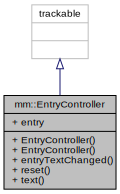
\includegraphics[width=192pt]{db/db6/structmm_1_1_entry_controller__coll__graph}
\end{center}
\end{figure}
\subsection*{Membri pubblici}
\begin{DoxyCompactItemize}
\item 
\mbox{\hyperlink{structmm_1_1_entry_controller_a8669618dd4526580cdb3cd88f9d16e52}{Entry\+Controller}} ()=delete
\item 
\mbox{\hyperlink{structmm_1_1_entry_controller_a8c99741ce10e997c35b397cef397fa6d}{Entry\+Controller}} (const std\+::string \&entry\+Id)
\item 
void \mbox{\hyperlink{structmm_1_1_entry_controller_ad4d3a1e3dc08262fe244e8c9bc0a455c}{entry\+Text\+Changed}} (const Glib\+::ustring \&, int $\ast$)
\item 
void \mbox{\hyperlink{structmm_1_1_entry_controller_a8eb56a968a567d1641c47d0f08b23f6f}{reset}} ()
\item 
std\+::string \mbox{\hyperlink{structmm_1_1_entry_controller_a8665e8b7d74b0f8c807d5b3ad418e535}{text}} ()
\end{DoxyCompactItemize}
\subsection*{Attributi pubblici}
\begin{DoxyCompactItemize}
\item 
Gtk\+::\+Entry $\ast$ \mbox{\hyperlink{structmm_1_1_entry_controller_ab41f377d1a98b2bf967c81dc1dc7f391}{entry}}
\end{DoxyCompactItemize}


\subsection{Documentazione dei costruttori e dei distruttori}
\mbox{\Hypertarget{structmm_1_1_entry_controller_a8669618dd4526580cdb3cd88f9d16e52}\label{structmm_1_1_entry_controller_a8669618dd4526580cdb3cd88f9d16e52}} 
\index{mm\+::\+Entry\+Controller@{mm\+::\+Entry\+Controller}!Entry\+Controller@{Entry\+Controller}}
\index{Entry\+Controller@{Entry\+Controller}!mm\+::\+Entry\+Controller@{mm\+::\+Entry\+Controller}}
\subsubsection{\texorpdfstring{Entry\+Controller()}{EntryController()}\hspace{0.1cm}{\footnotesize\ttfamily [1/2]}}
{\footnotesize\ttfamily mm\+::\+Entry\+Controller\+::\+Entry\+Controller (\begin{DoxyParamCaption}{ }\end{DoxyParamCaption})\hspace{0.3cm}{\ttfamily [delete]}}

\mbox{\Hypertarget{structmm_1_1_entry_controller_a8c99741ce10e997c35b397cef397fa6d}\label{structmm_1_1_entry_controller_a8c99741ce10e997c35b397cef397fa6d}} 
\index{mm\+::\+Entry\+Controller@{mm\+::\+Entry\+Controller}!Entry\+Controller@{Entry\+Controller}}
\index{Entry\+Controller@{Entry\+Controller}!mm\+::\+Entry\+Controller@{mm\+::\+Entry\+Controller}}
\subsubsection{\texorpdfstring{Entry\+Controller()}{EntryController()}\hspace{0.1cm}{\footnotesize\ttfamily [2/2]}}
{\footnotesize\ttfamily mm\+::\+Entry\+Controller\+::\+Entry\+Controller (\begin{DoxyParamCaption}\item[{const std\+::string \&}]{entry\+Id }\end{DoxyParamCaption})}



\subsection{Documentazione delle funzioni membro}
\mbox{\Hypertarget{structmm_1_1_entry_controller_ad4d3a1e3dc08262fe244e8c9bc0a455c}\label{structmm_1_1_entry_controller_ad4d3a1e3dc08262fe244e8c9bc0a455c}} 
\index{mm\+::\+Entry\+Controller@{mm\+::\+Entry\+Controller}!entry\+Text\+Changed@{entry\+Text\+Changed}}
\index{entry\+Text\+Changed@{entry\+Text\+Changed}!mm\+::\+Entry\+Controller@{mm\+::\+Entry\+Controller}}
\subsubsection{\texorpdfstring{entry\+Text\+Changed()}{entryTextChanged()}}
{\footnotesize\ttfamily void mm\+::\+Entry\+Controller\+::entry\+Text\+Changed (\begin{DoxyParamCaption}\item[{const Glib\+::ustring \&}]{,  }\item[{int $\ast$}]{ }\end{DoxyParamCaption})}

\mbox{\Hypertarget{structmm_1_1_entry_controller_a8eb56a968a567d1641c47d0f08b23f6f}\label{structmm_1_1_entry_controller_a8eb56a968a567d1641c47d0f08b23f6f}} 
\index{mm\+::\+Entry\+Controller@{mm\+::\+Entry\+Controller}!reset@{reset}}
\index{reset@{reset}!mm\+::\+Entry\+Controller@{mm\+::\+Entry\+Controller}}
\subsubsection{\texorpdfstring{reset()}{reset()}}
{\footnotesize\ttfamily void mm\+::\+Entry\+Controller\+::reset (\begin{DoxyParamCaption}{ }\end{DoxyParamCaption})\hspace{0.3cm}{\ttfamily [inline]}}

\mbox{\Hypertarget{structmm_1_1_entry_controller_a8665e8b7d74b0f8c807d5b3ad418e535}\label{structmm_1_1_entry_controller_a8665e8b7d74b0f8c807d5b3ad418e535}} 
\index{mm\+::\+Entry\+Controller@{mm\+::\+Entry\+Controller}!text@{text}}
\index{text@{text}!mm\+::\+Entry\+Controller@{mm\+::\+Entry\+Controller}}
\subsubsection{\texorpdfstring{text()}{text()}}
{\footnotesize\ttfamily std\+::string mm\+::\+Entry\+Controller\+::text (\begin{DoxyParamCaption}{ }\end{DoxyParamCaption})\hspace{0.3cm}{\ttfamily [inline]}}



\subsection{Documentazione dei membri dato}
\mbox{\Hypertarget{structmm_1_1_entry_controller_ab41f377d1a98b2bf967c81dc1dc7f391}\label{structmm_1_1_entry_controller_ab41f377d1a98b2bf967c81dc1dc7f391}} 
\index{mm\+::\+Entry\+Controller@{mm\+::\+Entry\+Controller}!entry@{entry}}
\index{entry@{entry}!mm\+::\+Entry\+Controller@{mm\+::\+Entry\+Controller}}
\subsubsection{\texorpdfstring{entry}{entry}}
{\footnotesize\ttfamily Gtk\+::\+Entry$\ast$ mm\+::\+Entry\+Controller\+::entry}



La documentazione per questa struct è stata generata a partire dai seguenti file\+:\begin{DoxyCompactItemize}
\item 
code/gui/\mbox{\hyperlink{_widgets_8hpp}{Widgets.\+hpp}}\item 
code/gui/\mbox{\hyperlink{_widgets_8cpp}{Widgets.\+cpp}}\end{DoxyCompactItemize}

\hypertarget{classmm_1_1view_1_1_interaction_entry}{}\section{Riferimenti per la classe mm\+:\+:view\+:\+:Interaction\+Entry}
\label{classmm_1_1view_1_1_interaction_entry}\index{mm\+::view\+::\+Interaction\+Entry@{mm\+::view\+::\+Interaction\+Entry}}


{\ttfamily \#include $<$Custom\+Widgets.\+hpp$>$}



Diagramma delle classi per mm\+:\+:view\+:\+:Interaction\+Entry
\nopagebreak
\begin{figure}[H]
\begin{center}
\leavevmode
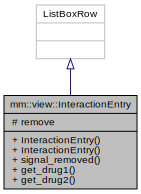
\includegraphics[width=214pt]{d9/dda/classmm_1_1view_1_1_interaction_entry__inherit__graph}
\end{center}
\end{figure}


Diagramma di collaborazione per mm\+:\+:view\+:\+:Interaction\+Entry\+:
\nopagebreak
\begin{figure}[H]
\begin{center}
\leavevmode
\includegraphics[width=214pt]{d0/d1d/classmm_1_1view_1_1_interaction_entry__coll__graph}
\end{center}
\end{figure}
\subsection*{Membri pubblici}
\begin{DoxyCompactItemize}
\item 
\mbox{\hyperlink{classmm_1_1view_1_1_interaction_entry_a6ee26295e5dd8871a0cf801014a8cc34}{Interaction\+Entry}} ()=delete
\item 
\mbox{\hyperlink{classmm_1_1view_1_1_interaction_entry_a1e3a924b7b218109d2df6b4ebbc557f0}{Interaction\+Entry}} (const Glib\+::ustring \&drug1, const Glib\+::ustring \&drug2)
\item 
sigc\+::signal$<$ void, \mbox{\hyperlink{classmm_1_1view_1_1_interaction_entry}{mm\+::view\+::\+Interaction\+Entry}} $\ast$ $>$ \mbox{\hyperlink{classmm_1_1view_1_1_interaction_entry_a48fc0d3c44a4d0b5364d822ebbdf07a1}{signal\+\_\+removed}} ()
\item 
const string \& \mbox{\hyperlink{classmm_1_1view_1_1_interaction_entry_a1f579cbaf213f6e602e8d2b67109a1c2}{get\+\_\+drug1}} () const
\item 
const string \& \mbox{\hyperlink{classmm_1_1view_1_1_interaction_entry_a58a4843226a5b149541eda7b1905eb85}{get\+\_\+drug2}} () const
\end{DoxyCompactItemize}
\subsection*{Attributi protetti}
\begin{DoxyCompactItemize}
\item 
sigc\+::signal$<$ void, \mbox{\hyperlink{classmm_1_1view_1_1_interaction_entry}{mm\+::view\+::\+Interaction\+Entry}} $\ast$ $>$ \mbox{\hyperlink{classmm_1_1view_1_1_interaction_entry_ac17d59c180df431cfffd90501d6845ef}{remove}}
\end{DoxyCompactItemize}


\subsection{Documentazione dei costruttori e dei distruttori}
\mbox{\Hypertarget{classmm_1_1view_1_1_interaction_entry_a6ee26295e5dd8871a0cf801014a8cc34}\label{classmm_1_1view_1_1_interaction_entry_a6ee26295e5dd8871a0cf801014a8cc34}} 
\index{mm\+::view\+::\+Interaction\+Entry@{mm\+::view\+::\+Interaction\+Entry}!Interaction\+Entry@{Interaction\+Entry}}
\index{Interaction\+Entry@{Interaction\+Entry}!mm\+::view\+::\+Interaction\+Entry@{mm\+::view\+::\+Interaction\+Entry}}
\subsubsection{\texorpdfstring{Interaction\+Entry()}{InteractionEntry()}\hspace{0.1cm}{\footnotesize\ttfamily [1/2]}}
{\footnotesize\ttfamily mm\+::view\+::\+Interaction\+Entry\+::\+Interaction\+Entry (\begin{DoxyParamCaption}{ }\end{DoxyParamCaption})\hspace{0.3cm}{\ttfamily [delete]}}

\mbox{\Hypertarget{classmm_1_1view_1_1_interaction_entry_a1e3a924b7b218109d2df6b4ebbc557f0}\label{classmm_1_1view_1_1_interaction_entry_a1e3a924b7b218109d2df6b4ebbc557f0}} 
\index{mm\+::view\+::\+Interaction\+Entry@{mm\+::view\+::\+Interaction\+Entry}!Interaction\+Entry@{Interaction\+Entry}}
\index{Interaction\+Entry@{Interaction\+Entry}!mm\+::view\+::\+Interaction\+Entry@{mm\+::view\+::\+Interaction\+Entry}}
\subsubsection{\texorpdfstring{Interaction\+Entry()}{InteractionEntry()}\hspace{0.1cm}{\footnotesize\ttfamily [2/2]}}
{\footnotesize\ttfamily mm\+::view\+::\+Interaction\+Entry\+::\+Interaction\+Entry (\begin{DoxyParamCaption}\item[{const Glib\+::ustring \&}]{drug1,  }\item[{const Glib\+::ustring \&}]{drug2 }\end{DoxyParamCaption})}



\subsection{Documentazione delle funzioni membro}
\mbox{\Hypertarget{classmm_1_1view_1_1_interaction_entry_a1f579cbaf213f6e602e8d2b67109a1c2}\label{classmm_1_1view_1_1_interaction_entry_a1f579cbaf213f6e602e8d2b67109a1c2}} 
\index{mm\+::view\+::\+Interaction\+Entry@{mm\+::view\+::\+Interaction\+Entry}!get\+\_\+drug1@{get\+\_\+drug1}}
\index{get\+\_\+drug1@{get\+\_\+drug1}!mm\+::view\+::\+Interaction\+Entry@{mm\+::view\+::\+Interaction\+Entry}}
\subsubsection{\texorpdfstring{get\+\_\+drug1()}{get\_drug1()}}
{\footnotesize\ttfamily const string \& mm\+::view\+::\+Interaction\+Entry\+::get\+\_\+drug1 (\begin{DoxyParamCaption}{ }\end{DoxyParamCaption}) const}

\mbox{\Hypertarget{classmm_1_1view_1_1_interaction_entry_a58a4843226a5b149541eda7b1905eb85}\label{classmm_1_1view_1_1_interaction_entry_a58a4843226a5b149541eda7b1905eb85}} 
\index{mm\+::view\+::\+Interaction\+Entry@{mm\+::view\+::\+Interaction\+Entry}!get\+\_\+drug2@{get\+\_\+drug2}}
\index{get\+\_\+drug2@{get\+\_\+drug2}!mm\+::view\+::\+Interaction\+Entry@{mm\+::view\+::\+Interaction\+Entry}}
\subsubsection{\texorpdfstring{get\+\_\+drug2()}{get\_drug2()}}
{\footnotesize\ttfamily const string \& mm\+::view\+::\+Interaction\+Entry\+::get\+\_\+drug2 (\begin{DoxyParamCaption}{ }\end{DoxyParamCaption}) const}

\mbox{\Hypertarget{classmm_1_1view_1_1_interaction_entry_a48fc0d3c44a4d0b5364d822ebbdf07a1}\label{classmm_1_1view_1_1_interaction_entry_a48fc0d3c44a4d0b5364d822ebbdf07a1}} 
\index{mm\+::view\+::\+Interaction\+Entry@{mm\+::view\+::\+Interaction\+Entry}!signal\+\_\+removed@{signal\+\_\+removed}}
\index{signal\+\_\+removed@{signal\+\_\+removed}!mm\+::view\+::\+Interaction\+Entry@{mm\+::view\+::\+Interaction\+Entry}}
\subsubsection{\texorpdfstring{signal\+\_\+removed()}{signal\_removed()}}
{\footnotesize\ttfamily sigc\+::signal$<$ void, \mbox{\hyperlink{classmm_1_1view_1_1_interaction_entry}{mm\+::view\+::\+Interaction\+Entry}} $\ast$ $>$ mm\+::view\+::\+Interaction\+Entry\+::signal\+\_\+removed (\begin{DoxyParamCaption}{ }\end{DoxyParamCaption})}



\subsection{Documentazione dei membri dato}
\mbox{\Hypertarget{classmm_1_1view_1_1_interaction_entry_ac17d59c180df431cfffd90501d6845ef}\label{classmm_1_1view_1_1_interaction_entry_ac17d59c180df431cfffd90501d6845ef}} 
\index{mm\+::view\+::\+Interaction\+Entry@{mm\+::view\+::\+Interaction\+Entry}!remove@{remove}}
\index{remove@{remove}!mm\+::view\+::\+Interaction\+Entry@{mm\+::view\+::\+Interaction\+Entry}}
\subsubsection{\texorpdfstring{remove}{remove}}
{\footnotesize\ttfamily sigc\+::signal$<$void, \mbox{\hyperlink{classmm_1_1view_1_1_interaction_entry}{mm\+::view\+::\+Interaction\+Entry}} $\ast$$>$ mm\+::view\+::\+Interaction\+Entry\+::remove\hspace{0.3cm}{\ttfamily [protected]}}



La documentazione per questa classe è stata generata a partire dai seguenti file\+:\begin{DoxyCompactItemize}
\item 
code/gui/view/\mbox{\hyperlink{_custom_widgets_8hpp}{Custom\+Widgets.\+hpp}}\item 
code/gui/view/\mbox{\hyperlink{_custom_widgets_8cpp}{Custom\+Widgets.\+cpp}}\end{DoxyCompactItemize}

\hypertarget{classmm_1_1_i_observer}{}\section{Riferimenti per la classe mm\+:\+:I\+Observer}
\label{classmm_1_1_i_observer}\index{mm\+::\+I\+Observer@{mm\+::\+I\+Observer}}


{\ttfamily \#include $<$I\+Observer.\+hpp$>$}



Diagramma delle classi per mm\+:\+:I\+Observer
\nopagebreak
\begin{figure}[H]
\begin{center}
\leavevmode
\includegraphics[width=350pt]{d4/dd5/classmm_1_1_i_observer__inherit__graph}
\end{center}
\end{figure}


Diagramma di collaborazione per mm\+:\+:I\+Observer\+:
\nopagebreak
\begin{figure}[H]
\begin{center}
\leavevmode
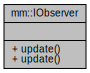
\includegraphics[width=162pt]{d7/d84/classmm_1_1_i_observer__coll__graph}
\end{center}
\end{figure}
\subsection*{Membri pubblici}
\begin{DoxyCompactItemize}
\item 
virtual void \mbox{\hyperlink{classmm_1_1_i_observer_a6422af04f8e9f3ba9d6d412a3bcdd03e}{update}} ()=0
\item 
virtual void \mbox{\hyperlink{classmm_1_1_i_observer_add1245a281c47575cc0e42449635a9fd}{update}} (unsigned int what)
\end{DoxyCompactItemize}


\subsection{Documentazione delle funzioni membro}
\mbox{\Hypertarget{classmm_1_1_i_observer_a6422af04f8e9f3ba9d6d412a3bcdd03e}\label{classmm_1_1_i_observer_a6422af04f8e9f3ba9d6d412a3bcdd03e}} 
\index{mm\+::\+I\+Observer@{mm\+::\+I\+Observer}!update@{update}}
\index{update@{update}!mm\+::\+I\+Observer@{mm\+::\+I\+Observer}}
\subsubsection{\texorpdfstring{update()}{update()}\hspace{0.1cm}{\footnotesize\ttfamily [1/2]}}
{\footnotesize\ttfamily virtual void mm\+::\+I\+Observer\+::update (\begin{DoxyParamCaption}{ }\end{DoxyParamCaption})\hspace{0.3cm}{\ttfamily [pure virtual]}}



Implementato in \mbox{\hyperlink{classmm_1_1_patient_window_a461de186f72a8902a9f95a622dc1c02b}{mm\+::\+Patient\+Window}}, \mbox{\hyperlink{classmm_1_1_main_window_ac0fc4875dc774c1b7b1ca59d174a7fc1}{mm\+::\+Main\+Window}}, \mbox{\hyperlink{classmm_1_1_drug_window_a98c6d97f491cb648dede0ef3db2b13b2}{mm\+::\+Drug\+Window}}, e \mbox{\hyperlink{classmm_1_1_prescription_window_a51195815f64b79179e3dafbb89b785e8}{mm\+::\+Prescription\+Window}}.

\mbox{\Hypertarget{classmm_1_1_i_observer_add1245a281c47575cc0e42449635a9fd}\label{classmm_1_1_i_observer_add1245a281c47575cc0e42449635a9fd}} 
\index{mm\+::\+I\+Observer@{mm\+::\+I\+Observer}!update@{update}}
\index{update@{update}!mm\+::\+I\+Observer@{mm\+::\+I\+Observer}}
\subsubsection{\texorpdfstring{update()}{update()}\hspace{0.1cm}{\footnotesize\ttfamily [2/2]}}
{\footnotesize\ttfamily virtual void mm\+::\+I\+Observer\+::update (\begin{DoxyParamCaption}\item[{unsigned int}]{what }\end{DoxyParamCaption})\hspace{0.3cm}{\ttfamily [inline]}, {\ttfamily [virtual]}}



Reimplementata in \mbox{\hyperlink{classmm_1_1_patient_window_a315f5e823a0261db4fb88b4e31333d53}{mm\+::\+Patient\+Window}}.



La documentazione per questa classe è stata generata a partire dal seguente file\+:\begin{DoxyCompactItemize}
\item 
code/interfaces/\mbox{\hyperlink{_i_observer_8hpp}{I\+Observer.\+hpp}}\end{DoxyCompactItemize}

\hypertarget{classmm_1_1_i_serializable}{}\section{Riferimenti per la classe mm\+:\+:I\+Serializable}
\label{classmm_1_1_i_serializable}\index{mm\+::\+I\+Serializable@{mm\+::\+I\+Serializable}}


Funziona come un interfaccia, qualunque classe che erediti da questa potrà essere letta o scritta nel database dal singleton \hyperlink{classmm_1_1_d_b_master}{D\+B\+Master}.  




{\ttfamily \#include $<$I\+Serializable.\+hpp$>$}



Diagramma delle classi per mm\+:\+:I\+Serializable\nopagebreak
\begin{figure}[H]
\begin{center}
\leavevmode
\includegraphics[width=350pt]{d5/d4e/classmm_1_1_i_serializable__inherit__graph}
\end{center}
\end{figure}


Diagramma di collaborazione per mm\+:\+:I\+Serializable\+:\nopagebreak
\begin{figure}[H]
\begin{center}
\leavevmode
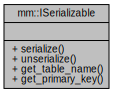
\includegraphics[width=185pt]{db/dc2/classmm_1_1_i_serializable__coll__graph}
\end{center}
\end{figure}
\subsection*{Membri pubblici}
\begin{DoxyCompactItemize}
\item 
virtual std\+::map$<$ std\+::string, \hyperlink{structmm_1_1_serialized}{Serialized} $>$ \hyperlink{classmm_1_1_i_serializable_a20a59e2324c8dbf6fefe4d11ae89d0fb}{serialize} () const =0
\item 
virtual void \hyperlink{classmm_1_1_i_serializable_a8e5329b3b23cd0dff0ea8f5f63bab996}{unserialize} (std\+::map$<$ std\+::string, \hyperlink{structmm_1_1_serialized}{Serialized} $>$)=0
\item 
virtual std\+::string \hyperlink{classmm_1_1_i_serializable_a9717e6da47fcbac3ffa2e68152464e0a}{get\+\_\+table\+\_\+name} () const =0
\item 
virtual std\+::vector$<$ std\+::string $>$ \hyperlink{classmm_1_1_i_serializable_a69c0c514e11e386b6cb1fbd03f14da17}{get\+\_\+primary\+\_\+key} () const =0
\end{DoxyCompactItemize}


\subsection{Descrizione dettagliata}
Funziona come un interfaccia, qualunque classe che erediti da questa potrà essere letta o scritta nel database dal singleton \hyperlink{classmm_1_1_d_b_master}{D\+B\+Master}. 

\subsection{Documentazione delle funzioni membro}
\mbox{\Hypertarget{classmm_1_1_i_serializable_a69c0c514e11e386b6cb1fbd03f14da17}\label{classmm_1_1_i_serializable_a69c0c514e11e386b6cb1fbd03f14da17}} 
\index{mm\+::\+I\+Serializable@{mm\+::\+I\+Serializable}!get\+\_\+primary\+\_\+key@{get\+\_\+primary\+\_\+key}}
\index{get\+\_\+primary\+\_\+key@{get\+\_\+primary\+\_\+key}!mm\+::\+I\+Serializable@{mm\+::\+I\+Serializable}}
\subsubsection{\texorpdfstring{get\+\_\+primary\+\_\+key()}{get\_primary\_key()}}
{\footnotesize\ttfamily virtual std\+::vector$<$std\+::string$>$ mm\+::\+I\+Serializable\+::get\+\_\+primary\+\_\+key (\begin{DoxyParamCaption}{ }\end{DoxyParamCaption}) const\hspace{0.3cm}{\ttfamily [pure virtual]}}



Implementato in \hyperlink{classmm_1_1model_1_1_doctor_a935989cbe2274076c2b409126d4faccd}{mm\+::model\+::\+Doctor}, \hyperlink{classmm_1_1model_1_1_drug_a019770ab95f95f34bbc204c4c3860bfa}{mm\+::model\+::\+Drug}, \hyperlink{classmm_1_1model_1_1_patient_ae85640f3cb3d34bb57e1129ef46a0cbf}{mm\+::model\+::\+Patient}, \hyperlink{classmm_1_1model_1_1_prescription_af521915f8872df18ae4a50ff2a4f59ff}{mm\+::model\+::\+Prescription}, e \hyperlink{structmm_1_1model_1_1authentication_1_1_login_a56f5da26be2d64baa78d0c81d99c8221}{mm\+::model\+::authentication\+::\+Login}.

\mbox{\Hypertarget{classmm_1_1_i_serializable_a9717e6da47fcbac3ffa2e68152464e0a}\label{classmm_1_1_i_serializable_a9717e6da47fcbac3ffa2e68152464e0a}} 
\index{mm\+::\+I\+Serializable@{mm\+::\+I\+Serializable}!get\+\_\+table\+\_\+name@{get\+\_\+table\+\_\+name}}
\index{get\+\_\+table\+\_\+name@{get\+\_\+table\+\_\+name}!mm\+::\+I\+Serializable@{mm\+::\+I\+Serializable}}
\subsubsection{\texorpdfstring{get\+\_\+table\+\_\+name()}{get\_table\_name()}}
{\footnotesize\ttfamily virtual std\+::string mm\+::\+I\+Serializable\+::get\+\_\+table\+\_\+name (\begin{DoxyParamCaption}{ }\end{DoxyParamCaption}) const\hspace{0.3cm}{\ttfamily [pure virtual]}}



Implementato in \hyperlink{classmm_1_1model_1_1_doctor_af4c37e48f9e5ff26f2295678f10afaa3}{mm\+::model\+::\+Doctor}, \hyperlink{classmm_1_1model_1_1_drug_a7fa9dbb569b89f397d4b865b778b3751}{mm\+::model\+::\+Drug}, \hyperlink{classmm_1_1model_1_1_patient_abe79da3e4fabd80e039ae4880dfa76cb}{mm\+::model\+::\+Patient}, \hyperlink{classmm_1_1model_1_1_prescription_a8de9a927dc92c0e0b15dac6f930889e3}{mm\+::model\+::\+Prescription}, e \hyperlink{structmm_1_1model_1_1authentication_1_1_login_afc72adef91be3d97ce4751b8a2357613}{mm\+::model\+::authentication\+::\+Login}.

\mbox{\Hypertarget{classmm_1_1_i_serializable_a20a59e2324c8dbf6fefe4d11ae89d0fb}\label{classmm_1_1_i_serializable_a20a59e2324c8dbf6fefe4d11ae89d0fb}} 
\index{mm\+::\+I\+Serializable@{mm\+::\+I\+Serializable}!serialize@{serialize}}
\index{serialize@{serialize}!mm\+::\+I\+Serializable@{mm\+::\+I\+Serializable}}
\subsubsection{\texorpdfstring{serialize()}{serialize()}}
{\footnotesize\ttfamily virtual std\+::map$<$std\+::string, \hyperlink{structmm_1_1_serialized}{Serialized}$>$ mm\+::\+I\+Serializable\+::serialize (\begin{DoxyParamCaption}{ }\end{DoxyParamCaption}) const\hspace{0.3cm}{\ttfamily [pure virtual]}}



Implementato in \hyperlink{classmm_1_1model_1_1_doctor_a2171a9cb9c8a24ad0c0331edae957910}{mm\+::model\+::\+Doctor}, \hyperlink{classmm_1_1model_1_1_drug_a5d4fa5bf5e4700f833547c5114764c7b}{mm\+::model\+::\+Drug}, \hyperlink{classmm_1_1model_1_1_patient_ae3ac219cd109e8c53daaf9b2758c3a0e}{mm\+::model\+::\+Patient}, \hyperlink{classmm_1_1model_1_1_prescription_a592ff88dfa9625a383a7b073a64863b1}{mm\+::model\+::\+Prescription}, e \hyperlink{structmm_1_1model_1_1authentication_1_1_login_a69ec1a769ef1659b8ed39d5e23c24333}{mm\+::model\+::authentication\+::\+Login}.

\mbox{\Hypertarget{classmm_1_1_i_serializable_a8e5329b3b23cd0dff0ea8f5f63bab996}\label{classmm_1_1_i_serializable_a8e5329b3b23cd0dff0ea8f5f63bab996}} 
\index{mm\+::\+I\+Serializable@{mm\+::\+I\+Serializable}!unserialize@{unserialize}}
\index{unserialize@{unserialize}!mm\+::\+I\+Serializable@{mm\+::\+I\+Serializable}}
\subsubsection{\texorpdfstring{unserialize()}{unserialize()}}
{\footnotesize\ttfamily virtual void mm\+::\+I\+Serializable\+::unserialize (\begin{DoxyParamCaption}\item[{std\+::map$<$ std\+::string, \hyperlink{structmm_1_1_serialized}{Serialized} $>$}]{ }\end{DoxyParamCaption})\hspace{0.3cm}{\ttfamily [pure virtual]}}



La documentazione per questa classe è stata generata a partire dal seguente file\+:\begin{DoxyCompactItemize}
\item 
code/interfaces/\hyperlink{_i_serializable_8hpp}{I\+Serializable.\+hpp}\end{DoxyCompactItemize}

\hypertarget{classmm_1_1_i_subject}{}\section{Riferimenti per la classe mm\+:\+:I\+Subject}
\label{classmm_1_1_i_subject}\index{mm\+::\+I\+Subject@{mm\+::\+I\+Subject}}


{\ttfamily \#include $<$I\+Subject.\+hpp$>$}



Diagramma delle classi per mm\+:\+:I\+Subject\nopagebreak
\begin{figure}[H]
\begin{center}
\leavevmode
\includegraphics[width=350pt]{da/d21/classmm_1_1_i_subject__inherit__graph}
\end{center}
\end{figure}


Diagramma di collaborazione per mm\+:\+:I\+Subject\+:\nopagebreak
\begin{figure}[H]
\begin{center}
\leavevmode
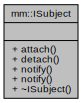
\includegraphics[width=154pt]{d6/dd5/classmm_1_1_i_subject__coll__graph}
\end{center}
\end{figure}
\subsection*{Membri pubblici}
\begin{DoxyCompactItemize}
\item 
void \hyperlink{classmm_1_1_i_subject_a76069d8db0c9c3d543154b0c2ce23bc9}{attach} (\hyperlink{classmm_1_1_i_observer}{I\+Observer} $\ast$obj) noexcept
\item 
void \hyperlink{classmm_1_1_i_subject_a64be1c0b2ad7ee4631a5270dedb7aa88}{detach} (\hyperlink{classmm_1_1_i_observer}{I\+Observer} $\ast$obj) noexcept(false)
\item 
void \hyperlink{classmm_1_1_i_subject_ad693fe5eb99bc20bc6d70f30bdf1140d}{notify} () const
\item 
virtual \hyperlink{classmm_1_1_i_subject_a37235a8b8ef83116c7351c56e17f7f57}{$\sim$\+I\+Subject} ()
\end{DoxyCompactItemize}


\subsection{Documentazione dei costruttori e dei distruttori}
\mbox{\Hypertarget{classmm_1_1_i_subject_a37235a8b8ef83116c7351c56e17f7f57}\label{classmm_1_1_i_subject_a37235a8b8ef83116c7351c56e17f7f57}} 
\index{mm\+::\+I\+Subject@{mm\+::\+I\+Subject}!````~I\+Subject@{$\sim$\+I\+Subject}}
\index{````~I\+Subject@{$\sim$\+I\+Subject}!mm\+::\+I\+Subject@{mm\+::\+I\+Subject}}
\subsubsection{\texorpdfstring{$\sim$\+I\+Subject()}{~ISubject()}}
{\footnotesize\ttfamily mm\+::\+I\+Subject\+::$\sim$\+I\+Subject (\begin{DoxyParamCaption}{ }\end{DoxyParamCaption})\hspace{0.3cm}{\ttfamily [virtual]}}



\subsection{Documentazione delle funzioni membro}
\mbox{\Hypertarget{classmm_1_1_i_subject_a76069d8db0c9c3d543154b0c2ce23bc9}\label{classmm_1_1_i_subject_a76069d8db0c9c3d543154b0c2ce23bc9}} 
\index{mm\+::\+I\+Subject@{mm\+::\+I\+Subject}!attach@{attach}}
\index{attach@{attach}!mm\+::\+I\+Subject@{mm\+::\+I\+Subject}}
\subsubsection{\texorpdfstring{attach()}{attach()}}
{\footnotesize\ttfamily void mm\+::\+I\+Subject\+::attach (\begin{DoxyParamCaption}\item[{\hyperlink{classmm_1_1_i_observer}{mm\+::\+I\+Observer} $\ast$}]{obj }\end{DoxyParamCaption})\hspace{0.3cm}{\ttfamily [noexcept]}}

\mbox{\Hypertarget{classmm_1_1_i_subject_a64be1c0b2ad7ee4631a5270dedb7aa88}\label{classmm_1_1_i_subject_a64be1c0b2ad7ee4631a5270dedb7aa88}} 
\index{mm\+::\+I\+Subject@{mm\+::\+I\+Subject}!detach@{detach}}
\index{detach@{detach}!mm\+::\+I\+Subject@{mm\+::\+I\+Subject}}
\subsubsection{\texorpdfstring{detach()}{detach()}}
{\footnotesize\ttfamily void mm\+::\+I\+Subject\+::detach (\begin{DoxyParamCaption}\item[{\hyperlink{classmm_1_1_i_observer}{mm\+::\+I\+Observer} $\ast$}]{obj }\end{DoxyParamCaption})\hspace{0.3cm}{\ttfamily [noexcept]}}

\mbox{\Hypertarget{classmm_1_1_i_subject_ad693fe5eb99bc20bc6d70f30bdf1140d}\label{classmm_1_1_i_subject_ad693fe5eb99bc20bc6d70f30bdf1140d}} 
\index{mm\+::\+I\+Subject@{mm\+::\+I\+Subject}!notify@{notify}}
\index{notify@{notify}!mm\+::\+I\+Subject@{mm\+::\+I\+Subject}}
\subsubsection{\texorpdfstring{notify()}{notify()}}
{\footnotesize\ttfamily void mm\+::\+I\+Subject\+::notify (\begin{DoxyParamCaption}{ }\end{DoxyParamCaption}) const}



La documentazione per questa classe è stata generata a partire dai seguenti file\+:\begin{DoxyCompactItemize}
\item 
code/interfaces/\hyperlink{_i_subject_8hpp}{I\+Subject.\+hpp}\item 
code/interfaces/\hyperlink{_i_subject_8cpp}{I\+Subject.\+cpp}\end{DoxyCompactItemize}

\hypertarget{classmm_1_1key__not__found__error}{}\section{Riferimenti per la classe mm\+:\+:key\+\_\+not\+\_\+found\+\_\+error}
\label{classmm_1_1key__not__found__error}\index{mm\+::key\+\_\+not\+\_\+found\+\_\+error@{mm\+::key\+\_\+not\+\_\+found\+\_\+error}}


Eccezione che indica che non è stata trovata una key nel file json.  




{\ttfamily \#include $<$Configuration.\+hpp$>$}



Diagramma delle classi per mm\+:\+:key\+\_\+not\+\_\+found\+\_\+error
\nopagebreak
\begin{figure}[H]
\begin{center}
\leavevmode
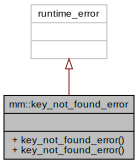
\includegraphics[width=211pt]{d4/de8/classmm_1_1key__not__found__error__inherit__graph}
\end{center}
\end{figure}


Diagramma di collaborazione per mm\+:\+:key\+\_\+not\+\_\+found\+\_\+error\+:
\nopagebreak
\begin{figure}[H]
\begin{center}
\leavevmode
\includegraphics[width=211pt]{d0/da9/classmm_1_1key__not__found__error__coll__graph}
\end{center}
\end{figure}
\subsection*{Membri pubblici}
\begin{DoxyCompactItemize}
\item 
\mbox{\hyperlink{classmm_1_1key__not__found__error_a2dbffa57a8ad2c3d80151f0d7b75814b}{key\+\_\+not\+\_\+found\+\_\+error}} (const std\+::string \&what)
\item 
\mbox{\hyperlink{classmm_1_1key__not__found__error_a650fb3f9d373793d9ba049e863eeef2d}{key\+\_\+not\+\_\+found\+\_\+error}} (const char $\ast$what)
\end{DoxyCompactItemize}


\subsection{Descrizione dettagliata}
Eccezione che indica che non è stata trovata una key nel file json. 

\subsection{Documentazione dei costruttori e dei distruttori}
\mbox{\Hypertarget{classmm_1_1key__not__found__error_a2dbffa57a8ad2c3d80151f0d7b75814b}\label{classmm_1_1key__not__found__error_a2dbffa57a8ad2c3d80151f0d7b75814b}} 
\index{mm\+::key\+\_\+not\+\_\+found\+\_\+error@{mm\+::key\+\_\+not\+\_\+found\+\_\+error}!key\+\_\+not\+\_\+found\+\_\+error@{key\+\_\+not\+\_\+found\+\_\+error}}
\index{key\+\_\+not\+\_\+found\+\_\+error@{key\+\_\+not\+\_\+found\+\_\+error}!mm\+::key\+\_\+not\+\_\+found\+\_\+error@{mm\+::key\+\_\+not\+\_\+found\+\_\+error}}
\subsubsection{\texorpdfstring{key\+\_\+not\+\_\+found\+\_\+error()}{key\_not\_found\_error()}\hspace{0.1cm}{\footnotesize\ttfamily [1/2]}}
{\footnotesize\ttfamily mm\+::key\+\_\+not\+\_\+found\+\_\+error\+::key\+\_\+not\+\_\+found\+\_\+error (\begin{DoxyParamCaption}\item[{const std\+::string \&}]{what }\end{DoxyParamCaption})}

\mbox{\Hypertarget{classmm_1_1key__not__found__error_a650fb3f9d373793d9ba049e863eeef2d}\label{classmm_1_1key__not__found__error_a650fb3f9d373793d9ba049e863eeef2d}} 
\index{mm\+::key\+\_\+not\+\_\+found\+\_\+error@{mm\+::key\+\_\+not\+\_\+found\+\_\+error}!key\+\_\+not\+\_\+found\+\_\+error@{key\+\_\+not\+\_\+found\+\_\+error}}
\index{key\+\_\+not\+\_\+found\+\_\+error@{key\+\_\+not\+\_\+found\+\_\+error}!mm\+::key\+\_\+not\+\_\+found\+\_\+error@{mm\+::key\+\_\+not\+\_\+found\+\_\+error}}
\subsubsection{\texorpdfstring{key\+\_\+not\+\_\+found\+\_\+error()}{key\_not\_found\_error()}\hspace{0.1cm}{\footnotesize\ttfamily [2/2]}}
{\footnotesize\ttfamily mm\+::key\+\_\+not\+\_\+found\+\_\+error\+::key\+\_\+not\+\_\+found\+\_\+error (\begin{DoxyParamCaption}\item[{const char $\ast$}]{what }\end{DoxyParamCaption})}



La documentazione per questa classe è stata generata a partire dai seguenti file\+:\begin{DoxyCompactItemize}
\item 
code/\mbox{\hyperlink{_configuration_8hpp}{Configuration.\+hpp}}\item 
code/\mbox{\hyperlink{_configuration_8cpp}{Configuration.\+cpp}}\end{DoxyCompactItemize}

\hypertarget{structmm_1_1model_1_1authentication_1_1_login}{}\section{Riferimenti per la struct mm\+:\+:model\+:\+:authentication\+:\+:Login}
\label{structmm_1_1model_1_1authentication_1_1_login}\index{mm\+::model\+::authentication\+::\+Login@{mm\+::model\+::authentication\+::\+Login}}


classe che rappresenta la una sessione di login  




{\ttfamily \#include $<$Authentication.\+hpp$>$}



Diagramma delle classi per mm\+:\+:model\+:\+:authentication\+:\+:Login
\nopagebreak
\begin{figure}[H]
\begin{center}
\leavevmode
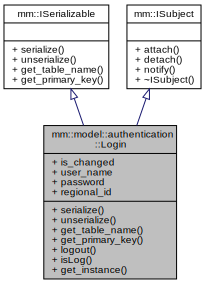
\includegraphics[width=278pt]{dc/d2d/structmm_1_1model_1_1authentication_1_1_login__inherit__graph}
\end{center}
\end{figure}


Diagramma di collaborazione per mm\+:\+:model\+:\+:authentication\+:\+:Login\+:
\nopagebreak
\begin{figure}[H]
\begin{center}
\leavevmode
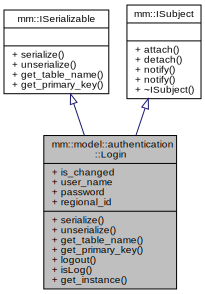
\includegraphics[width=278pt]{d8/dc8/structmm_1_1model_1_1authentication_1_1_login__coll__graph}
\end{center}
\end{figure}
\subsection*{Membri pubblici}
\begin{DoxyCompactItemize}
\item 
map$<$ string, \mbox{\hyperlink{structmm_1_1_serialized}{Serialized}} $>$ \mbox{\hyperlink{structmm_1_1model_1_1authentication_1_1_login_a69ec1a769ef1659b8ed39d5e23c24333}{serialize}} () const override
\item 
void \mbox{\hyperlink{structmm_1_1model_1_1authentication_1_1_login_ac2429ce08624b0c425feced836b77d62}{unserialize}} (map$<$ string, \mbox{\hyperlink{structmm_1_1_serialized}{Serialized}} $>$ map) override
\item 
string \mbox{\hyperlink{structmm_1_1model_1_1authentication_1_1_login_afc72adef91be3d97ce4751b8a2357613}{get\+\_\+table\+\_\+name}} () const override
\item 
vector$<$ string $>$ \mbox{\hyperlink{structmm_1_1model_1_1authentication_1_1_login_a56f5da26be2d64baa78d0c81d99c8221}{get\+\_\+primary\+\_\+key}} () const override
\item 
void \mbox{\hyperlink{structmm_1_1model_1_1authentication_1_1_login_a23843b088a1c1e0a668e9013ca6768ad}{logout}} ()
\begin{DoxyCompactList}\small\item\em Permette di effettuare il logout rendendo l\textquotesingle{}oggetto in uno stato non valido. \end{DoxyCompactList}\item 
bool \mbox{\hyperlink{structmm_1_1model_1_1authentication_1_1_login_aec29ca0fab75c7691c7939970646b39b}{is\+Log}} () const
\begin{DoxyCompactList}\small\item\em permette di controllare se l\textquotesingle{}oggetto è in uno stato valido o meno \end{DoxyCompactList}\end{DoxyCompactItemize}
\subsection*{Membri pubblici statici}
\begin{DoxyCompactItemize}
\item 
static \mbox{\hyperlink{structmm_1_1model_1_1authentication_1_1_login}{Login}} \& \mbox{\hyperlink{structmm_1_1model_1_1authentication_1_1_login_a37112a637ed012c96a96c5a2366f4220}{get\+\_\+instance}} ()
\begin{DoxyCompactList}\small\item\em Ritorna un istanza di tipo \mbox{\hyperlink{structmm_1_1model_1_1authentication_1_1_login}{Login}}. \end{DoxyCompactList}\end{DoxyCompactItemize}
\subsection*{Attributi pubblici}
\begin{DoxyCompactItemize}
\item 
bool \mbox{\hyperlink{structmm_1_1model_1_1authentication_1_1_login_aa74e292b2be0f1e2146576108e74db97}{is\+\_\+changed}}
\item 
std\+::string \mbox{\hyperlink{structmm_1_1model_1_1authentication_1_1_login_aeb7a295a6770bf778d747903045fe288}{user\+\_\+name}}
\item 
std\+::string \mbox{\hyperlink{structmm_1_1model_1_1authentication_1_1_login_adc6b1c53cf3e012f10c8b315a1df364f}{password}}
\item 
int \mbox{\hyperlink{structmm_1_1model_1_1authentication_1_1_login_a3b3c96185f5ad0c1e9ea15cd401ce064}{regional\+\_\+id}}
\end{DoxyCompactItemize}
\subsection*{Friend}
\begin{DoxyCompactItemize}
\item 
bool \mbox{\hyperlink{structmm_1_1model_1_1authentication_1_1_login_a5023cb987e79151f2a1ed18b9a86a3e8}{check\+\_\+login}} (std\+::string usr, std\+::string psw)
\begin{DoxyCompactList}\small\item\em Si occupa di porre in uno stato valido l\textquotesingle{}oggetto del singleton \mbox{\hyperlink{structmm_1_1model_1_1authentication_1_1_login}{Login}}. \end{DoxyCompactList}\end{DoxyCompactItemize}


\subsection{Descrizione dettagliata}
classe che rappresenta la una sessione di login 

Un oggetto di questo tipo può essere creato in modo solo dalla funzione check\+\_\+login se il login è già stato effettuato si può usare la funzione get\+\_\+instance per accedere ai dati relativi all\textquotesingle{}utente connesso, per sapere se la sessione è valida si può usare la funzione is\+Log. 

\subsection{Documentazione delle funzioni membro}
\mbox{\Hypertarget{structmm_1_1model_1_1authentication_1_1_login_a37112a637ed012c96a96c5a2366f4220}\label{structmm_1_1model_1_1authentication_1_1_login_a37112a637ed012c96a96c5a2366f4220}} 
\index{mm\+::model\+::authentication\+::\+Login@{mm\+::model\+::authentication\+::\+Login}!get\+\_\+instance@{get\+\_\+instance}}
\index{get\+\_\+instance@{get\+\_\+instance}!mm\+::model\+::authentication\+::\+Login@{mm\+::model\+::authentication\+::\+Login}}
\subsubsection{\texorpdfstring{get\+\_\+instance()}{get\_instance()}}
{\footnotesize\ttfamily \mbox{\hyperlink{structmm_1_1model_1_1authentication_1_1_login}{mm\+::model\+::authentication\+::\+Login}} \& mm\+::model\+::authentication\+::\+Login\+::get\+\_\+instance (\begin{DoxyParamCaption}{ }\end{DoxyParamCaption})\hspace{0.3cm}{\ttfamily [static]}}



Ritorna un istanza di tipo \mbox{\hyperlink{structmm_1_1model_1_1authentication_1_1_login}{Login}}. 

Se il login non è stato creato mediante la funzione check\+\_\+login L\textquotesingle{}oggetto ritornato sarà non valido e la funzione is\+Log su di esso ritornerà false

\begin{DoxyReturn}{Restituisce}
un oggetto di tipo \mbox{\hyperlink{structmm_1_1model_1_1authentication_1_1_login}{Login}} 
\end{DoxyReturn}
\mbox{\Hypertarget{structmm_1_1model_1_1authentication_1_1_login_a56f5da26be2d64baa78d0c81d99c8221}\label{structmm_1_1model_1_1authentication_1_1_login_a56f5da26be2d64baa78d0c81d99c8221}} 
\index{mm\+::model\+::authentication\+::\+Login@{mm\+::model\+::authentication\+::\+Login}!get\+\_\+primary\+\_\+key@{get\+\_\+primary\+\_\+key}}
\index{get\+\_\+primary\+\_\+key@{get\+\_\+primary\+\_\+key}!mm\+::model\+::authentication\+::\+Login@{mm\+::model\+::authentication\+::\+Login}}
\subsubsection{\texorpdfstring{get\+\_\+primary\+\_\+key()}{get\_primary\_key()}}
{\footnotesize\ttfamily vector$<$ string $>$ mm\+::model\+::authentication\+::\+Login\+::get\+\_\+primary\+\_\+key (\begin{DoxyParamCaption}{ }\end{DoxyParamCaption}) const\hspace{0.3cm}{\ttfamily [override]}, {\ttfamily [virtual]}}



Implementa \mbox{\hyperlink{classmm_1_1_i_serializable_a69c0c514e11e386b6cb1fbd03f14da17}{mm\+::\+I\+Serializable}}.

\mbox{\Hypertarget{structmm_1_1model_1_1authentication_1_1_login_afc72adef91be3d97ce4751b8a2357613}\label{structmm_1_1model_1_1authentication_1_1_login_afc72adef91be3d97ce4751b8a2357613}} 
\index{mm\+::model\+::authentication\+::\+Login@{mm\+::model\+::authentication\+::\+Login}!get\+\_\+table\+\_\+name@{get\+\_\+table\+\_\+name}}
\index{get\+\_\+table\+\_\+name@{get\+\_\+table\+\_\+name}!mm\+::model\+::authentication\+::\+Login@{mm\+::model\+::authentication\+::\+Login}}
\subsubsection{\texorpdfstring{get\+\_\+table\+\_\+name()}{get\_table\_name()}}
{\footnotesize\ttfamily string mm\+::model\+::authentication\+::\+Login\+::get\+\_\+table\+\_\+name (\begin{DoxyParamCaption}{ }\end{DoxyParamCaption}) const\hspace{0.3cm}{\ttfamily [override]}, {\ttfamily [virtual]}}



Implementa \mbox{\hyperlink{classmm_1_1_i_serializable_a9717e6da47fcbac3ffa2e68152464e0a}{mm\+::\+I\+Serializable}}.

\mbox{\Hypertarget{structmm_1_1model_1_1authentication_1_1_login_aec29ca0fab75c7691c7939970646b39b}\label{structmm_1_1model_1_1authentication_1_1_login_aec29ca0fab75c7691c7939970646b39b}} 
\index{mm\+::model\+::authentication\+::\+Login@{mm\+::model\+::authentication\+::\+Login}!is\+Log@{is\+Log}}
\index{is\+Log@{is\+Log}!mm\+::model\+::authentication\+::\+Login@{mm\+::model\+::authentication\+::\+Login}}
\subsubsection{\texorpdfstring{is\+Log()}{isLog()}}
{\footnotesize\ttfamily bool mm\+::model\+::authentication\+::\+Login\+::is\+Log (\begin{DoxyParamCaption}{ }\end{DoxyParamCaption}) const}



permette di controllare se l\textquotesingle{}oggetto è in uno stato valido o meno 

\begin{DoxyReturn}{Restituisce}
true se l\textquotesingle{}utente è connesso, false altrimenti 
\end{DoxyReturn}
\mbox{\Hypertarget{structmm_1_1model_1_1authentication_1_1_login_a23843b088a1c1e0a668e9013ca6768ad}\label{structmm_1_1model_1_1authentication_1_1_login_a23843b088a1c1e0a668e9013ca6768ad}} 
\index{mm\+::model\+::authentication\+::\+Login@{mm\+::model\+::authentication\+::\+Login}!logout@{logout}}
\index{logout@{logout}!mm\+::model\+::authentication\+::\+Login@{mm\+::model\+::authentication\+::\+Login}}
\subsubsection{\texorpdfstring{logout()}{logout()}}
{\footnotesize\ttfamily void mm\+::model\+::authentication\+::\+Login\+::logout (\begin{DoxyParamCaption}{ }\end{DoxyParamCaption})}



Permette di effettuare il logout rendendo l\textquotesingle{}oggetto in uno stato non valido. 

\mbox{\Hypertarget{structmm_1_1model_1_1authentication_1_1_login_a69ec1a769ef1659b8ed39d5e23c24333}\label{structmm_1_1model_1_1authentication_1_1_login_a69ec1a769ef1659b8ed39d5e23c24333}} 
\index{mm\+::model\+::authentication\+::\+Login@{mm\+::model\+::authentication\+::\+Login}!serialize@{serialize}}
\index{serialize@{serialize}!mm\+::model\+::authentication\+::\+Login@{mm\+::model\+::authentication\+::\+Login}}
\subsubsection{\texorpdfstring{serialize()}{serialize()}}
{\footnotesize\ttfamily map$<$ string, \mbox{\hyperlink{structmm_1_1_serialized}{mm\+::\+Serialized}} $>$ mm\+::model\+::authentication\+::\+Login\+::serialize (\begin{DoxyParamCaption}{ }\end{DoxyParamCaption}) const\hspace{0.3cm}{\ttfamily [override]}, {\ttfamily [virtual]}}



Implementa \mbox{\hyperlink{classmm_1_1_i_serializable_a20a59e2324c8dbf6fefe4d11ae89d0fb}{mm\+::\+I\+Serializable}}.

\mbox{\Hypertarget{structmm_1_1model_1_1authentication_1_1_login_ac2429ce08624b0c425feced836b77d62}\label{structmm_1_1model_1_1authentication_1_1_login_ac2429ce08624b0c425feced836b77d62}} 
\index{mm\+::model\+::authentication\+::\+Login@{mm\+::model\+::authentication\+::\+Login}!unserialize@{unserialize}}
\index{unserialize@{unserialize}!mm\+::model\+::authentication\+::\+Login@{mm\+::model\+::authentication\+::\+Login}}
\subsubsection{\texorpdfstring{unserialize()}{unserialize()}}
{\footnotesize\ttfamily void mm\+::model\+::authentication\+::\+Login\+::unserialize (\begin{DoxyParamCaption}\item[{map$<$ string, \mbox{\hyperlink{structmm_1_1_serialized}{Serialized}} $>$}]{map }\end{DoxyParamCaption})\hspace{0.3cm}{\ttfamily [override]}}



\subsection{Documentazione dei friend e delle funzioni collegate}
\mbox{\Hypertarget{structmm_1_1model_1_1authentication_1_1_login_a5023cb987e79151f2a1ed18b9a86a3e8}\label{structmm_1_1model_1_1authentication_1_1_login_a5023cb987e79151f2a1ed18b9a86a3e8}} 
\index{mm\+::model\+::authentication\+::\+Login@{mm\+::model\+::authentication\+::\+Login}!check\+\_\+login@{check\+\_\+login}}
\index{check\+\_\+login@{check\+\_\+login}!mm\+::model\+::authentication\+::\+Login@{mm\+::model\+::authentication\+::\+Login}}
\subsubsection{\texorpdfstring{check\+\_\+login}{check\_login}}
{\footnotesize\ttfamily bool check\+\_\+login (\begin{DoxyParamCaption}\item[{std\+::string}]{usr,  }\item[{std\+::string}]{psw }\end{DoxyParamCaption})\hspace{0.3cm}{\ttfamily [friend]}}



Si occupa di porre in uno stato valido l\textquotesingle{}oggetto del singleton \mbox{\hyperlink{structmm_1_1model_1_1authentication_1_1_login}{Login}}. 

Se usr e psw corrispondono ad una coppia nome utente e password nel database inizializza \mbox{\hyperlink{structmm_1_1model_1_1authentication_1_1_login}{Login}} e ritorna true


\begin{DoxyParams}{Parametri}
{\em usr} & stringa contenente lo username \\
\hline
{\em psw} & stringa contenente la password \\
\hline
\end{DoxyParams}
\begin{DoxyReturn}{Restituisce}
true in caso l\textquotesingle{}utente sia trovato false altrimenti 
\end{DoxyReturn}


\subsection{Documentazione dei membri dato}
\mbox{\Hypertarget{structmm_1_1model_1_1authentication_1_1_login_aa74e292b2be0f1e2146576108e74db97}\label{structmm_1_1model_1_1authentication_1_1_login_aa74e292b2be0f1e2146576108e74db97}} 
\index{mm\+::model\+::authentication\+::\+Login@{mm\+::model\+::authentication\+::\+Login}!is\+\_\+changed@{is\+\_\+changed}}
\index{is\+\_\+changed@{is\+\_\+changed}!mm\+::model\+::authentication\+::\+Login@{mm\+::model\+::authentication\+::\+Login}}
\subsubsection{\texorpdfstring{is\+\_\+changed}{is\_changed}}
{\footnotesize\ttfamily bool mm\+::model\+::authentication\+::\+Login\+::is\+\_\+changed}

\mbox{\Hypertarget{structmm_1_1model_1_1authentication_1_1_login_adc6b1c53cf3e012f10c8b315a1df364f}\label{structmm_1_1model_1_1authentication_1_1_login_adc6b1c53cf3e012f10c8b315a1df364f}} 
\index{mm\+::model\+::authentication\+::\+Login@{mm\+::model\+::authentication\+::\+Login}!password@{password}}
\index{password@{password}!mm\+::model\+::authentication\+::\+Login@{mm\+::model\+::authentication\+::\+Login}}
\subsubsection{\texorpdfstring{password}{password}}
{\footnotesize\ttfamily std\+::string mm\+::model\+::authentication\+::\+Login\+::password}

\mbox{\Hypertarget{structmm_1_1model_1_1authentication_1_1_login_a3b3c96185f5ad0c1e9ea15cd401ce064}\label{structmm_1_1model_1_1authentication_1_1_login_a3b3c96185f5ad0c1e9ea15cd401ce064}} 
\index{mm\+::model\+::authentication\+::\+Login@{mm\+::model\+::authentication\+::\+Login}!regional\+\_\+id@{regional\+\_\+id}}
\index{regional\+\_\+id@{regional\+\_\+id}!mm\+::model\+::authentication\+::\+Login@{mm\+::model\+::authentication\+::\+Login}}
\subsubsection{\texorpdfstring{regional\+\_\+id}{regional\_id}}
{\footnotesize\ttfamily int mm\+::model\+::authentication\+::\+Login\+::regional\+\_\+id}

\mbox{\Hypertarget{structmm_1_1model_1_1authentication_1_1_login_aeb7a295a6770bf778d747903045fe288}\label{structmm_1_1model_1_1authentication_1_1_login_aeb7a295a6770bf778d747903045fe288}} 
\index{mm\+::model\+::authentication\+::\+Login@{mm\+::model\+::authentication\+::\+Login}!user\+\_\+name@{user\+\_\+name}}
\index{user\+\_\+name@{user\+\_\+name}!mm\+::model\+::authentication\+::\+Login@{mm\+::model\+::authentication\+::\+Login}}
\subsubsection{\texorpdfstring{user\+\_\+name}{user\_name}}
{\footnotesize\ttfamily std\+::string mm\+::model\+::authentication\+::\+Login\+::user\+\_\+name}



La documentazione per questa struct è stata generata a partire dai seguenti file\+:\begin{DoxyCompactItemize}
\item 
code/model/\mbox{\hyperlink{_authentication_8hpp}{Authentication.\+hpp}}\item 
code/model/\mbox{\hyperlink{_authentication_8cpp}{Authentication.\+cpp}}\end{DoxyCompactItemize}

\hypertarget{classmm_1_1_login_window}{}\section{Riferimenti per la classe mm\+:\+:Login\+Window}
\label{classmm_1_1_login_window}\index{mm\+::\+Login\+Window@{mm\+::\+Login\+Window}}


{\ttfamily \#include $<$Login\+Window.\+hpp$>$}



Diagramma delle classi per mm\+:\+:Login\+Window
\nopagebreak
\begin{figure}[H]
\begin{center}
\leavevmode
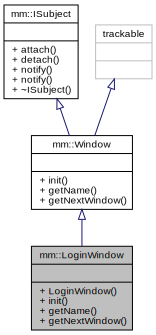
\includegraphics[width=228pt]{da/db3/classmm_1_1_login_window__inherit__graph}
\end{center}
\end{figure}


Diagramma di collaborazione per mm\+:\+:Login\+Window\+:
\nopagebreak
\begin{figure}[H]
\begin{center}
\leavevmode
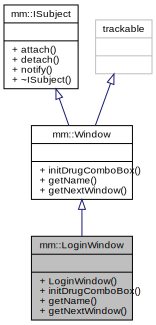
\includegraphics[width=228pt]{d7/de2/classmm_1_1_login_window__coll__graph}
\end{center}
\end{figure}
\subsection*{Membri pubblici}
\begin{DoxyCompactItemize}
\item 
\mbox{\hyperlink{classmm_1_1_login_window_ad27cc1365af4fec51bd7afb1a9d49cf5}{Login\+Window}} ()
\item 
bool \mbox{\hyperlink{classmm_1_1_login_window_a4040d7c1f85fc76e1f60ef13f92bef1c}{init}} () override
\item 
\mbox{\hyperlink{namespacemm_a4e9d92e04f65dbf2fc1963947da0d93c}{Window\+Name}} \mbox{\hyperlink{classmm_1_1_login_window_aa0597e725bfb2df984f526112080aaf7}{get\+Name}} () const override
\item 
\mbox{\hyperlink{namespacemm_a4e9d92e04f65dbf2fc1963947da0d93c}{Window\+Name}} \mbox{\hyperlink{classmm_1_1_login_window_a399eb7e1a310016ff83b7aa6a9d69722}{get\+Next\+Window}} () const override
\end{DoxyCompactItemize}


\subsection{Documentazione dei costruttori e dei distruttori}
\mbox{\Hypertarget{classmm_1_1_login_window_ad27cc1365af4fec51bd7afb1a9d49cf5}\label{classmm_1_1_login_window_ad27cc1365af4fec51bd7afb1a9d49cf5}} 
\index{mm\+::\+Login\+Window@{mm\+::\+Login\+Window}!Login\+Window@{Login\+Window}}
\index{Login\+Window@{Login\+Window}!mm\+::\+Login\+Window@{mm\+::\+Login\+Window}}
\subsubsection{\texorpdfstring{Login\+Window()}{LoginWindow()}}
{\footnotesize\ttfamily mm\+::\+Login\+Window\+::\+Login\+Window (\begin{DoxyParamCaption}{ }\end{DoxyParamCaption})}



\subsection{Documentazione delle funzioni membro}
\mbox{\Hypertarget{classmm_1_1_login_window_aa0597e725bfb2df984f526112080aaf7}\label{classmm_1_1_login_window_aa0597e725bfb2df984f526112080aaf7}} 
\index{mm\+::\+Login\+Window@{mm\+::\+Login\+Window}!get\+Name@{get\+Name}}
\index{get\+Name@{get\+Name}!mm\+::\+Login\+Window@{mm\+::\+Login\+Window}}
\subsubsection{\texorpdfstring{get\+Name()}{getName()}}
{\footnotesize\ttfamily \mbox{\hyperlink{namespacemm_a4e9d92e04f65dbf2fc1963947da0d93c}{mm\+::\+Window\+Name}} mm\+::\+Login\+Window\+::get\+Name (\begin{DoxyParamCaption}{ }\end{DoxyParamCaption}) const\hspace{0.3cm}{\ttfamily [override]}, {\ttfamily [virtual]}}



Implementa \mbox{\hyperlink{classmm_1_1_window_a942c9125bf42156a9f7b7f561e412fed}{mm\+::\+Window}}.

\mbox{\Hypertarget{classmm_1_1_login_window_a399eb7e1a310016ff83b7aa6a9d69722}\label{classmm_1_1_login_window_a399eb7e1a310016ff83b7aa6a9d69722}} 
\index{mm\+::\+Login\+Window@{mm\+::\+Login\+Window}!get\+Next\+Window@{get\+Next\+Window}}
\index{get\+Next\+Window@{get\+Next\+Window}!mm\+::\+Login\+Window@{mm\+::\+Login\+Window}}
\subsubsection{\texorpdfstring{get\+Next\+Window()}{getNextWindow()}}
{\footnotesize\ttfamily \mbox{\hyperlink{namespacemm_a4e9d92e04f65dbf2fc1963947da0d93c}{mm\+::\+Window\+Name}} mm\+::\+Login\+Window\+::get\+Next\+Window (\begin{DoxyParamCaption}{ }\end{DoxyParamCaption}) const\hspace{0.3cm}{\ttfamily [override]}, {\ttfamily [virtual]}}



Implementa \mbox{\hyperlink{classmm_1_1_window_a0cd7b4b0feb9505c44503547a161fcd8}{mm\+::\+Window}}.

\mbox{\Hypertarget{classmm_1_1_login_window_a4040d7c1f85fc76e1f60ef13f92bef1c}\label{classmm_1_1_login_window_a4040d7c1f85fc76e1f60ef13f92bef1c}} 
\index{mm\+::\+Login\+Window@{mm\+::\+Login\+Window}!init@{init}}
\index{init@{init}!mm\+::\+Login\+Window@{mm\+::\+Login\+Window}}
\subsubsection{\texorpdfstring{init()}{init()}}
{\footnotesize\ttfamily bool mm\+::\+Login\+Window\+::init (\begin{DoxyParamCaption}{ }\end{DoxyParamCaption})\hspace{0.3cm}{\ttfamily [override]}, {\ttfamily [virtual]}}



Implementa \mbox{\hyperlink{classmm_1_1_window_aba03fbf4761b2f106352baecf5996e10}{mm\+::\+Window}}.



La documentazione per questa classe è stata generata a partire dai seguenti file\+:\begin{DoxyCompactItemize}
\item 
code/gui/\mbox{\hyperlink{_login_window_8hpp}{Login\+Window.\+hpp}}\item 
code/gui/\mbox{\hyperlink{_login_window_8cpp}{Login\+Window.\+cpp}}\end{DoxyCompactItemize}

\hypertarget{classmm_1_1_main_window}{}\section{Riferimenti per la classe mm\+:\+:Main\+Window}
\label{classmm_1_1_main_window}\index{mm\+::\+Main\+Window@{mm\+::\+Main\+Window}}


{\ttfamily \#include $<$Main\+Window.\+hpp$>$}



Diagramma delle classi per mm\+:\+:Main\+Window
\nopagebreak
\begin{figure}[H]
\begin{center}
\leavevmode
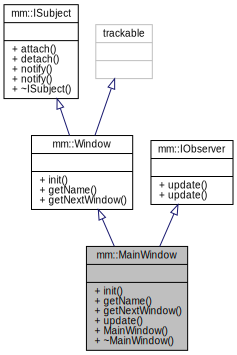
\includegraphics[width=309pt]{da/d0e/classmm_1_1_main_window__inherit__graph}
\end{center}
\end{figure}


Diagramma di collaborazione per mm\+:\+:Main\+Window\+:
\nopagebreak
\begin{figure}[H]
\begin{center}
\leavevmode
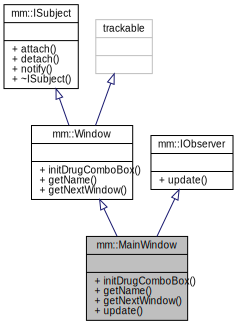
\includegraphics[width=309pt]{df/d8f/classmm_1_1_main_window__coll__graph}
\end{center}
\end{figure}
\subsection*{Membri pubblici}
\begin{DoxyCompactItemize}
\item 
bool \mbox{\hyperlink{classmm_1_1_main_window_a1094273a8ac991a50e4612efa8174fdd}{init}} () override
\item 
\mbox{\hyperlink{namespacemm_a4e9d92e04f65dbf2fc1963947da0d93c}{Window\+Name}} \mbox{\hyperlink{classmm_1_1_main_window_a8cfdfeb6ad47afff06fa6b1b7fdc0c88}{get\+Name}} () const override
\item 
\mbox{\hyperlink{namespacemm_a4e9d92e04f65dbf2fc1963947da0d93c}{Window\+Name}} \mbox{\hyperlink{classmm_1_1_main_window_aa1511ad7bed8d47cd35415d0a3a1161e}{get\+Next\+Window}} () const override
\item 
void \mbox{\hyperlink{classmm_1_1_main_window_ac0fc4875dc774c1b7b1ca59d174a7fc1}{update}} () override
\item 
\mbox{\hyperlink{classmm_1_1_main_window_ae9a06c62e4efd9fce7334afb032e20d6}{Main\+Window}} ()
\item 
virtual \mbox{\hyperlink{classmm_1_1_main_window_a37132df8fb730f15d8eb75f07e5fd92d}{$\sim$\+Main\+Window}} ()
\end{DoxyCompactItemize}


\subsection{Documentazione dei costruttori e dei distruttori}
\mbox{\Hypertarget{classmm_1_1_main_window_ae9a06c62e4efd9fce7334afb032e20d6}\label{classmm_1_1_main_window_ae9a06c62e4efd9fce7334afb032e20d6}} 
\index{mm\+::\+Main\+Window@{mm\+::\+Main\+Window}!Main\+Window@{Main\+Window}}
\index{Main\+Window@{Main\+Window}!mm\+::\+Main\+Window@{mm\+::\+Main\+Window}}
\subsubsection{\texorpdfstring{Main\+Window()}{MainWindow()}}
{\footnotesize\ttfamily mm\+::\+Main\+Window\+::\+Main\+Window (\begin{DoxyParamCaption}{ }\end{DoxyParamCaption})}

\mbox{\Hypertarget{classmm_1_1_main_window_a37132df8fb730f15d8eb75f07e5fd92d}\label{classmm_1_1_main_window_a37132df8fb730f15d8eb75f07e5fd92d}} 
\index{mm\+::\+Main\+Window@{mm\+::\+Main\+Window}!````~Main\+Window@{$\sim$\+Main\+Window}}
\index{````~Main\+Window@{$\sim$\+Main\+Window}!mm\+::\+Main\+Window@{mm\+::\+Main\+Window}}
\subsubsection{\texorpdfstring{$\sim$\+Main\+Window()}{~MainWindow()}}
{\footnotesize\ttfamily mm\+::\+Main\+Window\+::$\sim$\+Main\+Window (\begin{DoxyParamCaption}{ }\end{DoxyParamCaption})\hspace{0.3cm}{\ttfamily [virtual]}}



\subsection{Documentazione delle funzioni membro}
\mbox{\Hypertarget{classmm_1_1_main_window_a8cfdfeb6ad47afff06fa6b1b7fdc0c88}\label{classmm_1_1_main_window_a8cfdfeb6ad47afff06fa6b1b7fdc0c88}} 
\index{mm\+::\+Main\+Window@{mm\+::\+Main\+Window}!get\+Name@{get\+Name}}
\index{get\+Name@{get\+Name}!mm\+::\+Main\+Window@{mm\+::\+Main\+Window}}
\subsubsection{\texorpdfstring{get\+Name()}{getName()}}
{\footnotesize\ttfamily \mbox{\hyperlink{namespacemm_a4e9d92e04f65dbf2fc1963947da0d93c}{mm\+::\+Window\+Name}} mm\+::\+Main\+Window\+::get\+Name (\begin{DoxyParamCaption}{ }\end{DoxyParamCaption}) const\hspace{0.3cm}{\ttfamily [override]}, {\ttfamily [virtual]}}



Implementa \mbox{\hyperlink{classmm_1_1_window_a942c9125bf42156a9f7b7f561e412fed}{mm\+::\+Window}}.

\mbox{\Hypertarget{classmm_1_1_main_window_aa1511ad7bed8d47cd35415d0a3a1161e}\label{classmm_1_1_main_window_aa1511ad7bed8d47cd35415d0a3a1161e}} 
\index{mm\+::\+Main\+Window@{mm\+::\+Main\+Window}!get\+Next\+Window@{get\+Next\+Window}}
\index{get\+Next\+Window@{get\+Next\+Window}!mm\+::\+Main\+Window@{mm\+::\+Main\+Window}}
\subsubsection{\texorpdfstring{get\+Next\+Window()}{getNextWindow()}}
{\footnotesize\ttfamily \mbox{\hyperlink{namespacemm_a4e9d92e04f65dbf2fc1963947da0d93c}{mm\+::\+Window\+Name}} mm\+::\+Main\+Window\+::get\+Next\+Window (\begin{DoxyParamCaption}{ }\end{DoxyParamCaption}) const\hspace{0.3cm}{\ttfamily [override]}, {\ttfamily [virtual]}}



Implementa \mbox{\hyperlink{classmm_1_1_window_a0cd7b4b0feb9505c44503547a161fcd8}{mm\+::\+Window}}.

\mbox{\Hypertarget{classmm_1_1_main_window_a1094273a8ac991a50e4612efa8174fdd}\label{classmm_1_1_main_window_a1094273a8ac991a50e4612efa8174fdd}} 
\index{mm\+::\+Main\+Window@{mm\+::\+Main\+Window}!init@{init}}
\index{init@{init}!mm\+::\+Main\+Window@{mm\+::\+Main\+Window}}
\subsubsection{\texorpdfstring{init()}{init()}}
{\footnotesize\ttfamily bool mm\+::\+Main\+Window\+::init (\begin{DoxyParamCaption}{ }\end{DoxyParamCaption})\hspace{0.3cm}{\ttfamily [override]}, {\ttfamily [virtual]}}



Implementa \mbox{\hyperlink{classmm_1_1_window_aba03fbf4761b2f106352baecf5996e10}{mm\+::\+Window}}.

\mbox{\Hypertarget{classmm_1_1_main_window_ac0fc4875dc774c1b7b1ca59d174a7fc1}\label{classmm_1_1_main_window_ac0fc4875dc774c1b7b1ca59d174a7fc1}} 
\index{mm\+::\+Main\+Window@{mm\+::\+Main\+Window}!update@{update}}
\index{update@{update}!mm\+::\+Main\+Window@{mm\+::\+Main\+Window}}
\subsubsection{\texorpdfstring{update()}{update()}}
{\footnotesize\ttfamily void mm\+::\+Main\+Window\+::update (\begin{DoxyParamCaption}{ }\end{DoxyParamCaption})\hspace{0.3cm}{\ttfamily [override]}, {\ttfamily [virtual]}}



Implementa \mbox{\hyperlink{classmm_1_1_i_observer_a6422af04f8e9f3ba9d6d412a3bcdd03e}{mm\+::\+I\+Observer}}.



La documentazione per questa classe è stata generata a partire dai seguenti file\+:\begin{DoxyCompactItemize}
\item 
code/gui/\mbox{\hyperlink{_main_window_8hpp}{Main\+Window.\+hpp}}\item 
code/gui/\mbox{\hyperlink{_main_window_8cpp}{Main\+Window.\+cpp}}\end{DoxyCompactItemize}

\hypertarget{classmm_1_1_med_h}{}\section{Riferimenti per la classe mm\+:\+:MedH}
\label{classmm_1_1_med_h}\index{mm\+::\+MedH@{mm\+::\+MedH}}


Classe che rappresenta il programma in se.  




{\ttfamily \#include \char`\"{}Med\+H.\+hpp\char`\"{}}



Diagramma delle classi per mm\+:\+:MedH
\nopagebreak
\begin{figure}[H]
\begin{center}
\leavevmode
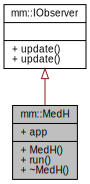
\includegraphics[width=162pt]{d3/d8f/classmm_1_1_med_h__inherit__graph}
\end{center}
\end{figure}


Diagramma di collaborazione per mm\+:\+:MedH\+:
\nopagebreak
\begin{figure}[H]
\begin{center}
\leavevmode
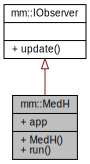
\includegraphics[width=162pt]{dc/d39/classmm_1_1_med_h__coll__graph}
\end{center}
\end{figure}
\subsection*{Membri pubblici}
\begin{DoxyCompactItemize}
\item 
\mbox{\hyperlink{classmm_1_1_med_h_a60861cff31fe5bc04e0002c6dabd5a9b}{MedH}} (int argc, char $\ast$$\ast$argv)
\item 
int \mbox{\hyperlink{classmm_1_1_med_h_aa34d2244a28a72dac6028e70317eb40b}{run}} ()
\begin{DoxyCompactList}\small\item\em lancia il main loop del programma. \end{DoxyCompactList}\item 
virtual \mbox{\hyperlink{classmm_1_1_med_h_a6fe53e9376821a1aae7d5a3a32d203c3}{$\sim$\+MedH}} ()
\end{DoxyCompactItemize}
\subsection*{Attributi pubblici}
\begin{DoxyCompactItemize}
\item 
Glib\+::\+Ref\+Ptr$<$ Gtk\+::\+Application $>$ \mbox{\hyperlink{classmm_1_1_med_h_a6bbf4476e1953d62562d35cb1f9c4218}{app}}
\end{DoxyCompactItemize}


\subsection{Descrizione dettagliata}
Classe che rappresenta il programma in se. 

Per utilizzare tutte le funzionalità del programma \mbox{\hyperlink{classmm_1_1_med_h}{MedH}} compresa l\textquotesingle{}interfaccia sarà necessario semplicemente creare un oggetto di \mbox{\hyperlink{classmm_1_1_med_h}{MedH}} e richiamarne il metodo run.

N.\+B. È possibile avviare più istanze dell\textquotesingle{}applicazione purché gli id nel config file siano diversi. 

\subsection{Documentazione dei costruttori e dei distruttori}
\mbox{\Hypertarget{classmm_1_1_med_h_a60861cff31fe5bc04e0002c6dabd5a9b}\label{classmm_1_1_med_h_a60861cff31fe5bc04e0002c6dabd5a9b}} 
\index{mm\+::\+MedH@{mm\+::\+MedH}!MedH@{MedH}}
\index{MedH@{MedH}!mm\+::\+MedH@{mm\+::\+MedH}}
\subsubsection{\texorpdfstring{Med\+H()}{MedH()}}
{\footnotesize\ttfamily mm\+::\+Med\+H\+::\+MedH (\begin{DoxyParamCaption}\item[{int}]{argc,  }\item[{char $\ast$$\ast$}]{argv }\end{DoxyParamCaption})}

\mbox{\Hypertarget{classmm_1_1_med_h_a6fe53e9376821a1aae7d5a3a32d203c3}\label{classmm_1_1_med_h_a6fe53e9376821a1aae7d5a3a32d203c3}} 
\index{mm\+::\+MedH@{mm\+::\+MedH}!````~MedH@{$\sim$\+MedH}}
\index{````~MedH@{$\sim$\+MedH}!mm\+::\+MedH@{mm\+::\+MedH}}
\subsubsection{\texorpdfstring{$\sim$\+Med\+H()}{~MedH()}}
{\footnotesize\ttfamily mm\+::\+Med\+H\+::$\sim$\+MedH (\begin{DoxyParamCaption}{ }\end{DoxyParamCaption})\hspace{0.3cm}{\ttfamily [virtual]}}



\subsection{Documentazione delle funzioni membro}
\mbox{\Hypertarget{classmm_1_1_med_h_aa34d2244a28a72dac6028e70317eb40b}\label{classmm_1_1_med_h_aa34d2244a28a72dac6028e70317eb40b}} 
\index{mm\+::\+MedH@{mm\+::\+MedH}!run@{run}}
\index{run@{run}!mm\+::\+MedH@{mm\+::\+MedH}}
\subsubsection{\texorpdfstring{run()}{run()}}
{\footnotesize\ttfamily int mm\+::\+Med\+H\+::run (\begin{DoxyParamCaption}{ }\end{DoxyParamCaption})}



lancia il main loop del programma. 



\subsection{Documentazione dei membri dato}
\mbox{\Hypertarget{classmm_1_1_med_h_a6bbf4476e1953d62562d35cb1f9c4218}\label{classmm_1_1_med_h_a6bbf4476e1953d62562d35cb1f9c4218}} 
\index{mm\+::\+MedH@{mm\+::\+MedH}!app@{app}}
\index{app@{app}!mm\+::\+MedH@{mm\+::\+MedH}}
\subsubsection{\texorpdfstring{app}{app}}
{\footnotesize\ttfamily Glib\+::\+Ref\+Ptr$<$Gtk\+::\+Application$>$ mm\+::\+Med\+H\+::app}



La documentazione per questa classe è stata generata a partire dai seguenti file\+:\begin{DoxyCompactItemize}
\item 
code/\mbox{\hyperlink{_med_h_8hpp}{Med\+H.\+hpp}}\item 
code/\mbox{\hyperlink{_med_h_8cpp}{Med\+H.\+cpp}}\end{DoxyCompactItemize}

\hypertarget{classmm_1_1observer__not__found__error}{}\section{Riferimenti per la classe mm\+:\+:observer\+\_\+not\+\_\+found\+\_\+error}
\label{classmm_1_1observer__not__found__error}\index{mm\+::observer\+\_\+not\+\_\+found\+\_\+error@{mm\+::observer\+\_\+not\+\_\+found\+\_\+error}}


{\ttfamily \#include $<$I\+Subject.\+hpp$>$}



Diagramma delle classi per mm\+:\+:observer\+\_\+not\+\_\+found\+\_\+error\nopagebreak
\begin{figure}[H]
\begin{center}
\leavevmode
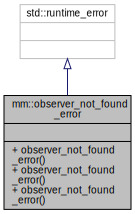
\includegraphics[width=207pt]{da/d02/classmm_1_1observer__not__found__error__inherit__graph}
\end{center}
\end{figure}


Diagramma di collaborazione per mm\+:\+:observer\+\_\+not\+\_\+found\+\_\+error\+:\nopagebreak
\begin{figure}[H]
\begin{center}
\leavevmode
\includegraphics[width=207pt]{d7/d18/classmm_1_1observer__not__found__error__coll__graph}
\end{center}
\end{figure}
\subsection*{Membri pubblici}
\begin{DoxyCompactItemize}
\item 
\hyperlink{classmm_1_1observer__not__found__error_a967227c100638d8d978f8ee3dd6c70b4}{observer\+\_\+not\+\_\+found\+\_\+error} (const std\+::string \&error)
\item 
\hyperlink{classmm_1_1observer__not__found__error_a7bf8977aad52f25ac981ec9b7c961ba0}{observer\+\_\+not\+\_\+found\+\_\+error} (const char $\ast$error)
\item 
\hyperlink{classmm_1_1observer__not__found__error_a60ab7d1412fcd906c7976e686f9b936b}{observer\+\_\+not\+\_\+found\+\_\+error} (const std\+::runtime\+\_\+error \&error)
\end{DoxyCompactItemize}


\subsection{Documentazione dei costruttori e dei distruttori}
\mbox{\Hypertarget{classmm_1_1observer__not__found__error_a967227c100638d8d978f8ee3dd6c70b4}\label{classmm_1_1observer__not__found__error_a967227c100638d8d978f8ee3dd6c70b4}} 
\index{mm\+::observer\+\_\+not\+\_\+found\+\_\+error@{mm\+::observer\+\_\+not\+\_\+found\+\_\+error}!observer\+\_\+not\+\_\+found\+\_\+error@{observer\+\_\+not\+\_\+found\+\_\+error}}
\index{observer\+\_\+not\+\_\+found\+\_\+error@{observer\+\_\+not\+\_\+found\+\_\+error}!mm\+::observer\+\_\+not\+\_\+found\+\_\+error@{mm\+::observer\+\_\+not\+\_\+found\+\_\+error}}
\subsubsection{\texorpdfstring{observer\+\_\+not\+\_\+found\+\_\+error()}{observer\_not\_found\_error()}\hspace{0.1cm}{\footnotesize\ttfamily [1/3]}}
{\footnotesize\ttfamily mm\+::observer\+\_\+not\+\_\+found\+\_\+error\+::observer\+\_\+not\+\_\+found\+\_\+error (\begin{DoxyParamCaption}\item[{const std\+::string \&}]{error }\end{DoxyParamCaption})}

\mbox{\Hypertarget{classmm_1_1observer__not__found__error_a7bf8977aad52f25ac981ec9b7c961ba0}\label{classmm_1_1observer__not__found__error_a7bf8977aad52f25ac981ec9b7c961ba0}} 
\index{mm\+::observer\+\_\+not\+\_\+found\+\_\+error@{mm\+::observer\+\_\+not\+\_\+found\+\_\+error}!observer\+\_\+not\+\_\+found\+\_\+error@{observer\+\_\+not\+\_\+found\+\_\+error}}
\index{observer\+\_\+not\+\_\+found\+\_\+error@{observer\+\_\+not\+\_\+found\+\_\+error}!mm\+::observer\+\_\+not\+\_\+found\+\_\+error@{mm\+::observer\+\_\+not\+\_\+found\+\_\+error}}
\subsubsection{\texorpdfstring{observer\+\_\+not\+\_\+found\+\_\+error()}{observer\_not\_found\_error()}\hspace{0.1cm}{\footnotesize\ttfamily [2/3]}}
{\footnotesize\ttfamily mm\+::observer\+\_\+not\+\_\+found\+\_\+error\+::observer\+\_\+not\+\_\+found\+\_\+error (\begin{DoxyParamCaption}\item[{const char $\ast$}]{error }\end{DoxyParamCaption})}

\mbox{\Hypertarget{classmm_1_1observer__not__found__error_a60ab7d1412fcd906c7976e686f9b936b}\label{classmm_1_1observer__not__found__error_a60ab7d1412fcd906c7976e686f9b936b}} 
\index{mm\+::observer\+\_\+not\+\_\+found\+\_\+error@{mm\+::observer\+\_\+not\+\_\+found\+\_\+error}!observer\+\_\+not\+\_\+found\+\_\+error@{observer\+\_\+not\+\_\+found\+\_\+error}}
\index{observer\+\_\+not\+\_\+found\+\_\+error@{observer\+\_\+not\+\_\+found\+\_\+error}!mm\+::observer\+\_\+not\+\_\+found\+\_\+error@{mm\+::observer\+\_\+not\+\_\+found\+\_\+error}}
\subsubsection{\texorpdfstring{observer\+\_\+not\+\_\+found\+\_\+error()}{observer\_not\_found\_error()}\hspace{0.1cm}{\footnotesize\ttfamily [3/3]}}
{\footnotesize\ttfamily mm\+::observer\+\_\+not\+\_\+found\+\_\+error\+::observer\+\_\+not\+\_\+found\+\_\+error (\begin{DoxyParamCaption}\item[{const std\+::runtime\+\_\+error \&}]{error }\end{DoxyParamCaption})}



La documentazione per questa classe è stata generata a partire dai seguenti file\+:\begin{DoxyCompactItemize}
\item 
code/interfaces/\hyperlink{_i_subject_8hpp}{I\+Subject.\+hpp}\item 
code/interfaces/\hyperlink{_i_subject_8cpp}{I\+Subject.\+cpp}\end{DoxyCompactItemize}

\hypertarget{classmm_1_1model_1_1_patient}{}\section{Riferimenti per la classe mm\+:\+:model\+:\+:Patient}
\label{classmm_1_1model_1_1_patient}\index{mm\+::model\+::\+Patient@{mm\+::model\+::\+Patient}}


{\ttfamily \#include $<$Patient.\+hpp$>$}



Diagramma delle classi per mm\+:\+:model\+:\+:Patient
\nopagebreak
\begin{figure}[H]
\begin{center}
\leavevmode
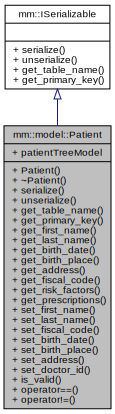
\includegraphics[width=187pt]{d0/d42/classmm_1_1model_1_1_patient__inherit__graph}
\end{center}
\end{figure}


Diagramma di collaborazione per mm\+:\+:model\+:\+:Patient\+:
\nopagebreak
\begin{figure}[H]
\begin{center}
\leavevmode
\includegraphics[height=550pt]{dc/d82/classmm_1_1model_1_1_patient__coll__graph}
\end{center}
\end{figure}
\subsection*{Composti}
\begin{DoxyCompactItemize}
\item 
struct \mbox{\hyperlink{structmm_1_1model_1_1_patient_1_1_tree_model}{Tree\+Model}}
\end{DoxyCompactItemize}
\subsection*{Membri pubblici}
\begin{DoxyCompactItemize}
\item 
\mbox{\hyperlink{classmm_1_1model_1_1_patient_ad15758bdb4995cf5f0b2830eef2b4b43}{Patient}} ()=default
\item 
\mbox{\hyperlink{classmm_1_1model_1_1_patient_ad9b2919b2efa8f1e7f6d405757d73ccb}{$\sim$\+Patient}} ()=default
\item 
map$<$ string, \mbox{\hyperlink{structmm_1_1_serialized}{Serialized}} $>$ \mbox{\hyperlink{classmm_1_1model_1_1_patient_ae3ac219cd109e8c53daaf9b2758c3a0e}{serialize}} () const override
\item 
void \mbox{\hyperlink{classmm_1_1model_1_1_patient_a7e1d8cbfc2cdd653281dce87497c6065}{unserialize}} (map$<$ string, \mbox{\hyperlink{structmm_1_1_serialized}{Serialized}} $>$ map) override
\item 
string \mbox{\hyperlink{classmm_1_1model_1_1_patient_abe79da3e4fabd80e039ae4880dfa76cb}{get\+\_\+table\+\_\+name}} () const override
\item 
vector$<$ string $>$ \mbox{\hyperlink{classmm_1_1model_1_1_patient_ae85640f3cb3d34bb57e1129ef46a0cbf}{get\+\_\+primary\+\_\+key}} () const override
\item 
const string \& \mbox{\hyperlink{classmm_1_1model_1_1_patient_a3661b2666d368492511ed3bad79c0389}{get\+\_\+first\+\_\+name}} () const
\item 
const string \& \mbox{\hyperlink{classmm_1_1model_1_1_patient_a88c0051957b5a6f172cdc35432505923}{get\+\_\+last\+\_\+name}} () const
\item 
const string \& \mbox{\hyperlink{classmm_1_1model_1_1_patient_ac54b024c619d6f31c72766a01bc5d0ee}{get\+\_\+birth\+\_\+date}} () const
\item 
const string \& \mbox{\hyperlink{classmm_1_1model_1_1_patient_a4e4770a79fef23b54026e013586e61fa}{get\+\_\+birth\+\_\+place}} () const
\item 
const string \& \mbox{\hyperlink{classmm_1_1model_1_1_patient_a0db04bf2c2ae5b9eb6417f4b6e74a84a}{get\+\_\+address}} () const
\item 
const string \& \mbox{\hyperlink{classmm_1_1model_1_1_patient_a29590c6ce9d2b19dbdff3330ee5e4523}{get\+\_\+fiscal\+\_\+code}} () const
\item 
string \mbox{\hyperlink{classmm_1_1model_1_1_patient_a7ab70bc4aafc95f687c29d02ac398e06}{get\+\_\+risk\+\_\+factors}} () const
\item 
vector$<$ \mbox{\hyperlink{classmm_1_1model_1_1_prescription}{Prescription}} $>$ \mbox{\hyperlink{classmm_1_1model_1_1_patient_ac13776eadc56f98bf353dd412f9c2f51}{get\+\_\+prescriptions}} () const
\item 
void \mbox{\hyperlink{classmm_1_1model_1_1_patient_a8b8dd8c6de5963a717cf192ca10c605e}{set\+\_\+first\+\_\+name}} (const string \&first\+\_\+name)
\item 
void \mbox{\hyperlink{classmm_1_1model_1_1_patient_a4883fc926a6693a2a6fd2b50ab2ded0e}{set\+\_\+last\+\_\+name}} (const string \&last\+\_\+name)
\item 
void \mbox{\hyperlink{classmm_1_1model_1_1_patient_a45485e586eb4a908ed4c7a51059fc131}{set\+\_\+fiscal\+\_\+code}} (const string \&fiscal\+\_\+code)
\item 
void \mbox{\hyperlink{classmm_1_1model_1_1_patient_ad73008977024e6ca48e5c687eb27b996}{set\+\_\+birth\+\_\+date}} (const string \&birth\+\_\+date)
\item 
void \mbox{\hyperlink{classmm_1_1model_1_1_patient_a6dc732f738425cc729764fdf16d667f0}{set\+\_\+birth\+\_\+place}} (const string \&birth\+\_\+place)
\item 
void \mbox{\hyperlink{classmm_1_1model_1_1_patient_a4e19f86233b55b4dec59f947f1dfe32a}{set\+\_\+address}} (const string \&address)
\item 
void \mbox{\hyperlink{classmm_1_1model_1_1_patient_a9dda6ce10296ab196cd5681b8e9a1091}{set\+\_\+doctor\+\_\+id}} (int doctor\+\_\+id)
\item 
bool \mbox{\hyperlink{classmm_1_1model_1_1_patient_a5f9da3f880ef1adc4bc5443ea407f48f}{is\+\_\+valid}} ()
\item 
bool \mbox{\hyperlink{classmm_1_1model_1_1_patient_a69367747ebc66b1b4e2fdf961811d83d}{operator==}} (const \mbox{\hyperlink{classmm_1_1model_1_1_patient}{Patient}} \&rhs) const
\item 
bool \mbox{\hyperlink{classmm_1_1model_1_1_patient_a96fe68d415c82b084ca75e87aefe8314}{operator!=}} (const \mbox{\hyperlink{classmm_1_1model_1_1_patient}{Patient}} \&rhs) const
\end{DoxyCompactItemize}
\subsection*{Attributi pubblici statici}
\begin{DoxyCompactItemize}
\item 
static \mbox{\hyperlink{structmm_1_1model_1_1_patient_1_1_tree_model}{Tree\+Model}} \mbox{\hyperlink{classmm_1_1model_1_1_patient_af2fe625b7bf2e3308df51daaff966281}{patient\+Tree\+Model}}
\end{DoxyCompactItemize}


\subsection{Documentazione dei costruttori e dei distruttori}
\mbox{\Hypertarget{classmm_1_1model_1_1_patient_ad15758bdb4995cf5f0b2830eef2b4b43}\label{classmm_1_1model_1_1_patient_ad15758bdb4995cf5f0b2830eef2b4b43}} 
\index{mm\+::model\+::\+Patient@{mm\+::model\+::\+Patient}!Patient@{Patient}}
\index{Patient@{Patient}!mm\+::model\+::\+Patient@{mm\+::model\+::\+Patient}}
\subsubsection{\texorpdfstring{Patient()}{Patient()}}
{\footnotesize\ttfamily mm\+::model\+::\+Patient\+::\+Patient (\begin{DoxyParamCaption}{ }\end{DoxyParamCaption})\hspace{0.3cm}{\ttfamily [default]}}

\mbox{\Hypertarget{classmm_1_1model_1_1_patient_ad9b2919b2efa8f1e7f6d405757d73ccb}\label{classmm_1_1model_1_1_patient_ad9b2919b2efa8f1e7f6d405757d73ccb}} 
\index{mm\+::model\+::\+Patient@{mm\+::model\+::\+Patient}!````~Patient@{$\sim$\+Patient}}
\index{````~Patient@{$\sim$\+Patient}!mm\+::model\+::\+Patient@{mm\+::model\+::\+Patient}}
\subsubsection{\texorpdfstring{$\sim$\+Patient()}{~Patient()}}
{\footnotesize\ttfamily mm\+::model\+::\+Patient\+::$\sim$\+Patient (\begin{DoxyParamCaption}{ }\end{DoxyParamCaption})\hspace{0.3cm}{\ttfamily [default]}}



\subsection{Documentazione delle funzioni membro}
\mbox{\Hypertarget{classmm_1_1model_1_1_patient_a0db04bf2c2ae5b9eb6417f4b6e74a84a}\label{classmm_1_1model_1_1_patient_a0db04bf2c2ae5b9eb6417f4b6e74a84a}} 
\index{mm\+::model\+::\+Patient@{mm\+::model\+::\+Patient}!get\+\_\+address@{get\+\_\+address}}
\index{get\+\_\+address@{get\+\_\+address}!mm\+::model\+::\+Patient@{mm\+::model\+::\+Patient}}
\subsubsection{\texorpdfstring{get\+\_\+address()}{get\_address()}}
{\footnotesize\ttfamily const string \& mm\+::model\+::\+Patient\+::get\+\_\+address (\begin{DoxyParamCaption}{ }\end{DoxyParamCaption}) const}

\mbox{\Hypertarget{classmm_1_1model_1_1_patient_ac54b024c619d6f31c72766a01bc5d0ee}\label{classmm_1_1model_1_1_patient_ac54b024c619d6f31c72766a01bc5d0ee}} 
\index{mm\+::model\+::\+Patient@{mm\+::model\+::\+Patient}!get\+\_\+birth\+\_\+date@{get\+\_\+birth\+\_\+date}}
\index{get\+\_\+birth\+\_\+date@{get\+\_\+birth\+\_\+date}!mm\+::model\+::\+Patient@{mm\+::model\+::\+Patient}}
\subsubsection{\texorpdfstring{get\+\_\+birth\+\_\+date()}{get\_birth\_date()}}
{\footnotesize\ttfamily const string \& mm\+::model\+::\+Patient\+::get\+\_\+birth\+\_\+date (\begin{DoxyParamCaption}{ }\end{DoxyParamCaption}) const}

\mbox{\Hypertarget{classmm_1_1model_1_1_patient_a4e4770a79fef23b54026e013586e61fa}\label{classmm_1_1model_1_1_patient_a4e4770a79fef23b54026e013586e61fa}} 
\index{mm\+::model\+::\+Patient@{mm\+::model\+::\+Patient}!get\+\_\+birth\+\_\+place@{get\+\_\+birth\+\_\+place}}
\index{get\+\_\+birth\+\_\+place@{get\+\_\+birth\+\_\+place}!mm\+::model\+::\+Patient@{mm\+::model\+::\+Patient}}
\subsubsection{\texorpdfstring{get\+\_\+birth\+\_\+place()}{get\_birth\_place()}}
{\footnotesize\ttfamily const string \& mm\+::model\+::\+Patient\+::get\+\_\+birth\+\_\+place (\begin{DoxyParamCaption}{ }\end{DoxyParamCaption}) const}

\mbox{\Hypertarget{classmm_1_1model_1_1_patient_a3661b2666d368492511ed3bad79c0389}\label{classmm_1_1model_1_1_patient_a3661b2666d368492511ed3bad79c0389}} 
\index{mm\+::model\+::\+Patient@{mm\+::model\+::\+Patient}!get\+\_\+first\+\_\+name@{get\+\_\+first\+\_\+name}}
\index{get\+\_\+first\+\_\+name@{get\+\_\+first\+\_\+name}!mm\+::model\+::\+Patient@{mm\+::model\+::\+Patient}}
\subsubsection{\texorpdfstring{get\+\_\+first\+\_\+name()}{get\_first\_name()}}
{\footnotesize\ttfamily const string \& mm\+::model\+::\+Patient\+::get\+\_\+first\+\_\+name (\begin{DoxyParamCaption}{ }\end{DoxyParamCaption}) const}

\mbox{\Hypertarget{classmm_1_1model_1_1_patient_a29590c6ce9d2b19dbdff3330ee5e4523}\label{classmm_1_1model_1_1_patient_a29590c6ce9d2b19dbdff3330ee5e4523}} 
\index{mm\+::model\+::\+Patient@{mm\+::model\+::\+Patient}!get\+\_\+fiscal\+\_\+code@{get\+\_\+fiscal\+\_\+code}}
\index{get\+\_\+fiscal\+\_\+code@{get\+\_\+fiscal\+\_\+code}!mm\+::model\+::\+Patient@{mm\+::model\+::\+Patient}}
\subsubsection{\texorpdfstring{get\+\_\+fiscal\+\_\+code()}{get\_fiscal\_code()}}
{\footnotesize\ttfamily const string \& mm\+::model\+::\+Patient\+::get\+\_\+fiscal\+\_\+code (\begin{DoxyParamCaption}{ }\end{DoxyParamCaption}) const}

\mbox{\Hypertarget{classmm_1_1model_1_1_patient_a88c0051957b5a6f172cdc35432505923}\label{classmm_1_1model_1_1_patient_a88c0051957b5a6f172cdc35432505923}} 
\index{mm\+::model\+::\+Patient@{mm\+::model\+::\+Patient}!get\+\_\+last\+\_\+name@{get\+\_\+last\+\_\+name}}
\index{get\+\_\+last\+\_\+name@{get\+\_\+last\+\_\+name}!mm\+::model\+::\+Patient@{mm\+::model\+::\+Patient}}
\subsubsection{\texorpdfstring{get\+\_\+last\+\_\+name()}{get\_last\_name()}}
{\footnotesize\ttfamily const string \& mm\+::model\+::\+Patient\+::get\+\_\+last\+\_\+name (\begin{DoxyParamCaption}{ }\end{DoxyParamCaption}) const}

\mbox{\Hypertarget{classmm_1_1model_1_1_patient_ac13776eadc56f98bf353dd412f9c2f51}\label{classmm_1_1model_1_1_patient_ac13776eadc56f98bf353dd412f9c2f51}} 
\index{mm\+::model\+::\+Patient@{mm\+::model\+::\+Patient}!get\+\_\+prescriptions@{get\+\_\+prescriptions}}
\index{get\+\_\+prescriptions@{get\+\_\+prescriptions}!mm\+::model\+::\+Patient@{mm\+::model\+::\+Patient}}
\subsubsection{\texorpdfstring{get\+\_\+prescriptions()}{get\_prescriptions()}}
{\footnotesize\ttfamily vector$<$ \mbox{\hyperlink{classmm_1_1model_1_1_prescription}{mm\+::model\+::\+Prescription}} $>$ mm\+::model\+::\+Patient\+::get\+\_\+prescriptions (\begin{DoxyParamCaption}{ }\end{DoxyParamCaption}) const}

\mbox{\Hypertarget{classmm_1_1model_1_1_patient_ae85640f3cb3d34bb57e1129ef46a0cbf}\label{classmm_1_1model_1_1_patient_ae85640f3cb3d34bb57e1129ef46a0cbf}} 
\index{mm\+::model\+::\+Patient@{mm\+::model\+::\+Patient}!get\+\_\+primary\+\_\+key@{get\+\_\+primary\+\_\+key}}
\index{get\+\_\+primary\+\_\+key@{get\+\_\+primary\+\_\+key}!mm\+::model\+::\+Patient@{mm\+::model\+::\+Patient}}
\subsubsection{\texorpdfstring{get\+\_\+primary\+\_\+key()}{get\_primary\_key()}}
{\footnotesize\ttfamily vector$<$ string $>$ mm\+::model\+::\+Patient\+::get\+\_\+primary\+\_\+key (\begin{DoxyParamCaption}{ }\end{DoxyParamCaption}) const\hspace{0.3cm}{\ttfamily [override]}, {\ttfamily [virtual]}}



Implementa \mbox{\hyperlink{classmm_1_1_i_serializable_a69c0c514e11e386b6cb1fbd03f14da17}{mm\+::\+I\+Serializable}}.

\mbox{\Hypertarget{classmm_1_1model_1_1_patient_a7ab70bc4aafc95f687c29d02ac398e06}\label{classmm_1_1model_1_1_patient_a7ab70bc4aafc95f687c29d02ac398e06}} 
\index{mm\+::model\+::\+Patient@{mm\+::model\+::\+Patient}!get\+\_\+risk\+\_\+factors@{get\+\_\+risk\+\_\+factors}}
\index{get\+\_\+risk\+\_\+factors@{get\+\_\+risk\+\_\+factors}!mm\+::model\+::\+Patient@{mm\+::model\+::\+Patient}}
\subsubsection{\texorpdfstring{get\+\_\+risk\+\_\+factors()}{get\_risk\_factors()}}
{\footnotesize\ttfamily string mm\+::model\+::\+Patient\+::get\+\_\+risk\+\_\+factors (\begin{DoxyParamCaption}{ }\end{DoxyParamCaption}) const}

\mbox{\Hypertarget{classmm_1_1model_1_1_patient_abe79da3e4fabd80e039ae4880dfa76cb}\label{classmm_1_1model_1_1_patient_abe79da3e4fabd80e039ae4880dfa76cb}} 
\index{mm\+::model\+::\+Patient@{mm\+::model\+::\+Patient}!get\+\_\+table\+\_\+name@{get\+\_\+table\+\_\+name}}
\index{get\+\_\+table\+\_\+name@{get\+\_\+table\+\_\+name}!mm\+::model\+::\+Patient@{mm\+::model\+::\+Patient}}
\subsubsection{\texorpdfstring{get\+\_\+table\+\_\+name()}{get\_table\_name()}}
{\footnotesize\ttfamily string mm\+::model\+::\+Patient\+::get\+\_\+table\+\_\+name (\begin{DoxyParamCaption}{ }\end{DoxyParamCaption}) const\hspace{0.3cm}{\ttfamily [override]}, {\ttfamily [virtual]}}



Implementa \mbox{\hyperlink{classmm_1_1_i_serializable_a9717e6da47fcbac3ffa2e68152464e0a}{mm\+::\+I\+Serializable}}.

\mbox{\Hypertarget{classmm_1_1model_1_1_patient_a5f9da3f880ef1adc4bc5443ea407f48f}\label{classmm_1_1model_1_1_patient_a5f9da3f880ef1adc4bc5443ea407f48f}} 
\index{mm\+::model\+::\+Patient@{mm\+::model\+::\+Patient}!is\+\_\+valid@{is\+\_\+valid}}
\index{is\+\_\+valid@{is\+\_\+valid}!mm\+::model\+::\+Patient@{mm\+::model\+::\+Patient}}
\subsubsection{\texorpdfstring{is\+\_\+valid()}{is\_valid()}}
{\footnotesize\ttfamily bool mm\+::model\+::\+Patient\+::is\+\_\+valid (\begin{DoxyParamCaption}{ }\end{DoxyParamCaption})}

\mbox{\Hypertarget{classmm_1_1model_1_1_patient_a96fe68d415c82b084ca75e87aefe8314}\label{classmm_1_1model_1_1_patient_a96fe68d415c82b084ca75e87aefe8314}} 
\index{mm\+::model\+::\+Patient@{mm\+::model\+::\+Patient}!operator"!=@{operator"!=}}
\index{operator"!=@{operator"!=}!mm\+::model\+::\+Patient@{mm\+::model\+::\+Patient}}
\subsubsection{\texorpdfstring{operator"!=()}{operator!=()}}
{\footnotesize\ttfamily bool mm\+::model\+::\+Patient\+::operator!= (\begin{DoxyParamCaption}\item[{const \mbox{\hyperlink{classmm_1_1model_1_1_patient}{Patient}} \&}]{rhs }\end{DoxyParamCaption}) const}

\mbox{\Hypertarget{classmm_1_1model_1_1_patient_a69367747ebc66b1b4e2fdf961811d83d}\label{classmm_1_1model_1_1_patient_a69367747ebc66b1b4e2fdf961811d83d}} 
\index{mm\+::model\+::\+Patient@{mm\+::model\+::\+Patient}!operator==@{operator==}}
\index{operator==@{operator==}!mm\+::model\+::\+Patient@{mm\+::model\+::\+Patient}}
\subsubsection{\texorpdfstring{operator==()}{operator==()}}
{\footnotesize\ttfamily bool mm\+::model\+::\+Patient\+::operator== (\begin{DoxyParamCaption}\item[{const \mbox{\hyperlink{classmm_1_1model_1_1_patient}{Patient}} \&}]{rhs }\end{DoxyParamCaption}) const}

\mbox{\Hypertarget{classmm_1_1model_1_1_patient_ae3ac219cd109e8c53daaf9b2758c3a0e}\label{classmm_1_1model_1_1_patient_ae3ac219cd109e8c53daaf9b2758c3a0e}} 
\index{mm\+::model\+::\+Patient@{mm\+::model\+::\+Patient}!serialize@{serialize}}
\index{serialize@{serialize}!mm\+::model\+::\+Patient@{mm\+::model\+::\+Patient}}
\subsubsection{\texorpdfstring{serialize()}{serialize()}}
{\footnotesize\ttfamily map$<$ string, \mbox{\hyperlink{structmm_1_1_serialized}{mm\+::\+Serialized}} $>$ mm\+::model\+::\+Patient\+::serialize (\begin{DoxyParamCaption}{ }\end{DoxyParamCaption}) const\hspace{0.3cm}{\ttfamily [override]}, {\ttfamily [virtual]}}



Implementa \mbox{\hyperlink{classmm_1_1_i_serializable_a20a59e2324c8dbf6fefe4d11ae89d0fb}{mm\+::\+I\+Serializable}}.

\mbox{\Hypertarget{classmm_1_1model_1_1_patient_a4e19f86233b55b4dec59f947f1dfe32a}\label{classmm_1_1model_1_1_patient_a4e19f86233b55b4dec59f947f1dfe32a}} 
\index{mm\+::model\+::\+Patient@{mm\+::model\+::\+Patient}!set\+\_\+address@{set\+\_\+address}}
\index{set\+\_\+address@{set\+\_\+address}!mm\+::model\+::\+Patient@{mm\+::model\+::\+Patient}}
\subsubsection{\texorpdfstring{set\+\_\+address()}{set\_address()}}
{\footnotesize\ttfamily void mm\+::model\+::\+Patient\+::set\+\_\+address (\begin{DoxyParamCaption}\item[{const string \&}]{address }\end{DoxyParamCaption})}

\mbox{\Hypertarget{classmm_1_1model_1_1_patient_ad73008977024e6ca48e5c687eb27b996}\label{classmm_1_1model_1_1_patient_ad73008977024e6ca48e5c687eb27b996}} 
\index{mm\+::model\+::\+Patient@{mm\+::model\+::\+Patient}!set\+\_\+birth\+\_\+date@{set\+\_\+birth\+\_\+date}}
\index{set\+\_\+birth\+\_\+date@{set\+\_\+birth\+\_\+date}!mm\+::model\+::\+Patient@{mm\+::model\+::\+Patient}}
\subsubsection{\texorpdfstring{set\+\_\+birth\+\_\+date()}{set\_birth\_date()}}
{\footnotesize\ttfamily void mm\+::model\+::\+Patient\+::set\+\_\+birth\+\_\+date (\begin{DoxyParamCaption}\item[{const string \&}]{birth\+\_\+date }\end{DoxyParamCaption})}

\mbox{\Hypertarget{classmm_1_1model_1_1_patient_a6dc732f738425cc729764fdf16d667f0}\label{classmm_1_1model_1_1_patient_a6dc732f738425cc729764fdf16d667f0}} 
\index{mm\+::model\+::\+Patient@{mm\+::model\+::\+Patient}!set\+\_\+birth\+\_\+place@{set\+\_\+birth\+\_\+place}}
\index{set\+\_\+birth\+\_\+place@{set\+\_\+birth\+\_\+place}!mm\+::model\+::\+Patient@{mm\+::model\+::\+Patient}}
\subsubsection{\texorpdfstring{set\+\_\+birth\+\_\+place()}{set\_birth\_place()}}
{\footnotesize\ttfamily void mm\+::model\+::\+Patient\+::set\+\_\+birth\+\_\+place (\begin{DoxyParamCaption}\item[{const string \&}]{birth\+\_\+place }\end{DoxyParamCaption})}

\mbox{\Hypertarget{classmm_1_1model_1_1_patient_a9dda6ce10296ab196cd5681b8e9a1091}\label{classmm_1_1model_1_1_patient_a9dda6ce10296ab196cd5681b8e9a1091}} 
\index{mm\+::model\+::\+Patient@{mm\+::model\+::\+Patient}!set\+\_\+doctor\+\_\+id@{set\+\_\+doctor\+\_\+id}}
\index{set\+\_\+doctor\+\_\+id@{set\+\_\+doctor\+\_\+id}!mm\+::model\+::\+Patient@{mm\+::model\+::\+Patient}}
\subsubsection{\texorpdfstring{set\+\_\+doctor\+\_\+id()}{set\_doctor\_id()}}
{\footnotesize\ttfamily void mm\+::model\+::\+Patient\+::set\+\_\+doctor\+\_\+id (\begin{DoxyParamCaption}\item[{int}]{doctor\+\_\+id }\end{DoxyParamCaption})}

\mbox{\Hypertarget{classmm_1_1model_1_1_patient_a8b8dd8c6de5963a717cf192ca10c605e}\label{classmm_1_1model_1_1_patient_a8b8dd8c6de5963a717cf192ca10c605e}} 
\index{mm\+::model\+::\+Patient@{mm\+::model\+::\+Patient}!set\+\_\+first\+\_\+name@{set\+\_\+first\+\_\+name}}
\index{set\+\_\+first\+\_\+name@{set\+\_\+first\+\_\+name}!mm\+::model\+::\+Patient@{mm\+::model\+::\+Patient}}
\subsubsection{\texorpdfstring{set\+\_\+first\+\_\+name()}{set\_first\_name()}}
{\footnotesize\ttfamily void mm\+::model\+::\+Patient\+::set\+\_\+first\+\_\+name (\begin{DoxyParamCaption}\item[{const string \&}]{first\+\_\+name }\end{DoxyParamCaption})}

\mbox{\Hypertarget{classmm_1_1model_1_1_patient_a45485e586eb4a908ed4c7a51059fc131}\label{classmm_1_1model_1_1_patient_a45485e586eb4a908ed4c7a51059fc131}} 
\index{mm\+::model\+::\+Patient@{mm\+::model\+::\+Patient}!set\+\_\+fiscal\+\_\+code@{set\+\_\+fiscal\+\_\+code}}
\index{set\+\_\+fiscal\+\_\+code@{set\+\_\+fiscal\+\_\+code}!mm\+::model\+::\+Patient@{mm\+::model\+::\+Patient}}
\subsubsection{\texorpdfstring{set\+\_\+fiscal\+\_\+code()}{set\_fiscal\_code()}}
{\footnotesize\ttfamily void mm\+::model\+::\+Patient\+::set\+\_\+fiscal\+\_\+code (\begin{DoxyParamCaption}\item[{const string \&}]{fiscal\+\_\+code }\end{DoxyParamCaption})}

\mbox{\Hypertarget{classmm_1_1model_1_1_patient_a4883fc926a6693a2a6fd2b50ab2ded0e}\label{classmm_1_1model_1_1_patient_a4883fc926a6693a2a6fd2b50ab2ded0e}} 
\index{mm\+::model\+::\+Patient@{mm\+::model\+::\+Patient}!set\+\_\+last\+\_\+name@{set\+\_\+last\+\_\+name}}
\index{set\+\_\+last\+\_\+name@{set\+\_\+last\+\_\+name}!mm\+::model\+::\+Patient@{mm\+::model\+::\+Patient}}
\subsubsection{\texorpdfstring{set\+\_\+last\+\_\+name()}{set\_last\_name()}}
{\footnotesize\ttfamily void mm\+::model\+::\+Patient\+::set\+\_\+last\+\_\+name (\begin{DoxyParamCaption}\item[{const string \&}]{last\+\_\+name }\end{DoxyParamCaption})}

\mbox{\Hypertarget{classmm_1_1model_1_1_patient_a7e1d8cbfc2cdd653281dce87497c6065}\label{classmm_1_1model_1_1_patient_a7e1d8cbfc2cdd653281dce87497c6065}} 
\index{mm\+::model\+::\+Patient@{mm\+::model\+::\+Patient}!unserialize@{unserialize}}
\index{unserialize@{unserialize}!mm\+::model\+::\+Patient@{mm\+::model\+::\+Patient}}
\subsubsection{\texorpdfstring{unserialize()}{unserialize()}}
{\footnotesize\ttfamily void mm\+::model\+::\+Patient\+::unserialize (\begin{DoxyParamCaption}\item[{map$<$ string, \mbox{\hyperlink{structmm_1_1_serialized}{Serialized}} $>$}]{map }\end{DoxyParamCaption})\hspace{0.3cm}{\ttfamily [override]}}



\subsection{Documentazione dei membri dato}
\mbox{\Hypertarget{classmm_1_1model_1_1_patient_af2fe625b7bf2e3308df51daaff966281}\label{classmm_1_1model_1_1_patient_af2fe625b7bf2e3308df51daaff966281}} 
\index{mm\+::model\+::\+Patient@{mm\+::model\+::\+Patient}!patient\+Tree\+Model@{patient\+Tree\+Model}}
\index{patient\+Tree\+Model@{patient\+Tree\+Model}!mm\+::model\+::\+Patient@{mm\+::model\+::\+Patient}}
\subsubsection{\texorpdfstring{patient\+Tree\+Model}{patientTreeModel}}
{\footnotesize\ttfamily \mbox{\hyperlink{structmm_1_1model_1_1_patient_1_1_tree_model}{mm\+::model\+::\+Patient\+::\+Tree\+Model}} mm\+::model\+::\+Patient\+::patient\+Tree\+Model\hspace{0.3cm}{\ttfamily [static]}}

Project Elaborato\+\_\+\+I\+N\+G\+\_\+\+SW \begin{DoxyAuthor}{Autore}
Noè Murr, Mirko Morati 
\end{DoxyAuthor}


La documentazione per questa classe è stata generata a partire dai seguenti file\+:\begin{DoxyCompactItemize}
\item 
code/model/\mbox{\hyperlink{_patient_8hpp}{Patient.\+hpp}}\item 
code/model/\mbox{\hyperlink{_patient_8cpp}{Patient.\+cpp}}\end{DoxyCompactItemize}

\hypertarget{classmm_1_1view_1_1_patient_expander}{}\section{Riferimenti per la classe mm\+:\+:view\+:\+:Patient\+Expander}
\label{classmm_1_1view_1_1_patient_expander}\index{mm\+::view\+::\+Patient\+Expander@{mm\+::view\+::\+Patient\+Expander}}


{\ttfamily \#include $<$Custom\+Widgets.\+hpp$>$}



Diagramma delle classi per mm\+:\+:view\+:\+:Patient\+Expander
\nopagebreak
\begin{figure}[H]
\begin{center}
\leavevmode
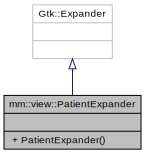
\includegraphics[width=218pt]{d0/d9d/classmm_1_1view_1_1_patient_expander__inherit__graph}
\end{center}
\end{figure}


Diagramma di collaborazione per mm\+:\+:view\+:\+:Patient\+Expander\+:
\nopagebreak
\begin{figure}[H]
\begin{center}
\leavevmode
\includegraphics[width=218pt]{d2/d15/classmm_1_1view_1_1_patient_expander__coll__graph}
\end{center}
\end{figure}
\subsection*{Membri pubblici}
\begin{DoxyCompactItemize}
\item 
\mbox{\hyperlink{classmm_1_1view_1_1_patient_expander_a07daa447ceef9466613982c707d62eed}{Patient\+Expander}} (const \mbox{\hyperlink{classmm_1_1model_1_1_patient}{mm\+::model\+::\+Patient}} \&patient, const \mbox{\hyperlink{classmm_1_1model_1_1_drug}{mm\+::model\+::\+Drug}} \&drug, const \mbox{\hyperlink{structmm_1_1util_1_1_date}{mm\+::util\+::\+Date}} \&start=\mbox{\hyperlink{structmm_1_1util_1_1_date_af0758fad7ef32fd535db3295136466eb}{mm\+::util\+::\+Date\+::get\+\_\+current\+\_\+date}}(), const \mbox{\hyperlink{structmm_1_1util_1_1_date}{mm\+::util\+::\+Date}} \&end=\mbox{\hyperlink{structmm_1_1util_1_1_date_af0758fad7ef32fd535db3295136466eb}{mm\+::util\+::\+Date\+::get\+\_\+current\+\_\+date}}())
\end{DoxyCompactItemize}


\subsection{Documentazione dei costruttori e dei distruttori}
\mbox{\Hypertarget{classmm_1_1view_1_1_patient_expander_a07daa447ceef9466613982c707d62eed}\label{classmm_1_1view_1_1_patient_expander_a07daa447ceef9466613982c707d62eed}} 
\index{mm\+::view\+::\+Patient\+Expander@{mm\+::view\+::\+Patient\+Expander}!Patient\+Expander@{Patient\+Expander}}
\index{Patient\+Expander@{Patient\+Expander}!mm\+::view\+::\+Patient\+Expander@{mm\+::view\+::\+Patient\+Expander}}
\subsubsection{\texorpdfstring{Patient\+Expander()}{PatientExpander()}}
{\footnotesize\ttfamily mm\+::view\+::\+Patient\+Expander\+::\+Patient\+Expander (\begin{DoxyParamCaption}\item[{const \mbox{\hyperlink{classmm_1_1model_1_1_patient}{mm\+::model\+::\+Patient}} \&}]{patient,  }\item[{const \mbox{\hyperlink{classmm_1_1model_1_1_drug}{mm\+::model\+::\+Drug}} \&}]{drug,  }\item[{const \mbox{\hyperlink{structmm_1_1util_1_1_date}{mm\+::util\+::\+Date}} \&}]{start = {\ttfamily \mbox{\hyperlink{structmm_1_1util_1_1_date_af0758fad7ef32fd535db3295136466eb}{mm\+::util\+::\+Date\+::get\+\_\+current\+\_\+date}}()},  }\item[{const \mbox{\hyperlink{structmm_1_1util_1_1_date}{mm\+::util\+::\+Date}} \&}]{end = {\ttfamily \mbox{\hyperlink{structmm_1_1util_1_1_date_af0758fad7ef32fd535db3295136466eb}{mm\+::util\+::\+Date\+::get\+\_\+current\+\_\+date}}()} }\end{DoxyParamCaption})}



La documentazione per questa classe è stata generata a partire dai seguenti file\+:\begin{DoxyCompactItemize}
\item 
code/gui/view/\mbox{\hyperlink{_custom_widgets_8hpp}{Custom\+Widgets.\+hpp}}\item 
code/gui/view/\mbox{\hyperlink{_custom_widgets_8cpp}{Custom\+Widgets.\+cpp}}\end{DoxyCompactItemize}

\hypertarget{classmm_1_1_patient_window}{}\section{Riferimenti per la classe mm\+:\+:Patient\+Window}
\label{classmm_1_1_patient_window}\index{mm\+::\+Patient\+Window@{mm\+::\+Patient\+Window}}


{\ttfamily \#include $<$Patient\+Window.\+hpp$>$}



Diagramma delle classi per mm\+:\+:Patient\+Window
\nopagebreak
\begin{figure}[H]
\begin{center}
\leavevmode
\includegraphics[width=309pt]{d9/d55/classmm_1_1_patient_window__inherit__graph}
\end{center}
\end{figure}


Diagramma di collaborazione per mm\+:\+:Patient\+Window\+:
\nopagebreak
\begin{figure}[H]
\begin{center}
\leavevmode
\includegraphics[width=309pt]{d2/da5/classmm_1_1_patient_window__coll__graph}
\end{center}
\end{figure}
\subsection*{Membri pubblici}
\begin{DoxyCompactItemize}
\item 
\mbox{\hyperlink{classmm_1_1_patient_window_a303da04da191185a070454feff15e014}{Patient\+Window}} ()
\item 
bool \mbox{\hyperlink{classmm_1_1_patient_window_a0ad27245769b095559858eeecdbb7089}{init}} () override
\item 
\mbox{\hyperlink{namespacemm_a4e9d92e04f65dbf2fc1963947da0d93c}{Window\+Name}} \mbox{\hyperlink{classmm_1_1_patient_window_ab951ab5bf21df2b9450496c6faca5268}{get\+Name}} () const override
\item 
\mbox{\hyperlink{namespacemm_a4e9d92e04f65dbf2fc1963947da0d93c}{Window\+Name}} \mbox{\hyperlink{classmm_1_1_patient_window_ae22b9bce4c7ccdbcc45feb080088a558}{get\+Next\+Window}} () const override
\item 
void \mbox{\hyperlink{classmm_1_1_patient_window_a461de186f72a8902a9f95a622dc1c02b}{update}} () override
\item 
void \mbox{\hyperlink{classmm_1_1_patient_window_a315f5e823a0261db4fb88b4e31333d53}{update}} (unsigned int what) override
\item 
\mbox{\hyperlink{classmm_1_1_patient_window_a48de0e9302eb9cb9b33e8641f27f01c1}{$\sim$\+Patient\+Window}} () override
\end{DoxyCompactItemize}


\subsection{Documentazione dei costruttori e dei distruttori}
\mbox{\Hypertarget{classmm_1_1_patient_window_a303da04da191185a070454feff15e014}\label{classmm_1_1_patient_window_a303da04da191185a070454feff15e014}} 
\index{mm\+::\+Patient\+Window@{mm\+::\+Patient\+Window}!Patient\+Window@{Patient\+Window}}
\index{Patient\+Window@{Patient\+Window}!mm\+::\+Patient\+Window@{mm\+::\+Patient\+Window}}
\subsubsection{\texorpdfstring{Patient\+Window()}{PatientWindow()}}
{\footnotesize\ttfamily mm\+::\+Patient\+Window\+::\+Patient\+Window (\begin{DoxyParamCaption}{ }\end{DoxyParamCaption})}

\mbox{\Hypertarget{classmm_1_1_patient_window_a48de0e9302eb9cb9b33e8641f27f01c1}\label{classmm_1_1_patient_window_a48de0e9302eb9cb9b33e8641f27f01c1}} 
\index{mm\+::\+Patient\+Window@{mm\+::\+Patient\+Window}!````~Patient\+Window@{$\sim$\+Patient\+Window}}
\index{````~Patient\+Window@{$\sim$\+Patient\+Window}!mm\+::\+Patient\+Window@{mm\+::\+Patient\+Window}}
\subsubsection{\texorpdfstring{$\sim$\+Patient\+Window()}{~PatientWindow()}}
{\footnotesize\ttfamily mm\+::\+Patient\+Window\+::$\sim$\+Patient\+Window (\begin{DoxyParamCaption}{ }\end{DoxyParamCaption})\hspace{0.3cm}{\ttfamily [override]}}



\subsection{Documentazione delle funzioni membro}
\mbox{\Hypertarget{classmm_1_1_patient_window_ab951ab5bf21df2b9450496c6faca5268}\label{classmm_1_1_patient_window_ab951ab5bf21df2b9450496c6faca5268}} 
\index{mm\+::\+Patient\+Window@{mm\+::\+Patient\+Window}!get\+Name@{get\+Name}}
\index{get\+Name@{get\+Name}!mm\+::\+Patient\+Window@{mm\+::\+Patient\+Window}}
\subsubsection{\texorpdfstring{get\+Name()}{getName()}}
{\footnotesize\ttfamily \mbox{\hyperlink{namespacemm_a4e9d92e04f65dbf2fc1963947da0d93c}{mm\+::\+Window\+Name}} mm\+::\+Patient\+Window\+::get\+Name (\begin{DoxyParamCaption}{ }\end{DoxyParamCaption}) const\hspace{0.3cm}{\ttfamily [override]}, {\ttfamily [virtual]}}



Implementa \mbox{\hyperlink{classmm_1_1_window_a942c9125bf42156a9f7b7f561e412fed}{mm\+::\+Window}}.

\mbox{\Hypertarget{classmm_1_1_patient_window_ae22b9bce4c7ccdbcc45feb080088a558}\label{classmm_1_1_patient_window_ae22b9bce4c7ccdbcc45feb080088a558}} 
\index{mm\+::\+Patient\+Window@{mm\+::\+Patient\+Window}!get\+Next\+Window@{get\+Next\+Window}}
\index{get\+Next\+Window@{get\+Next\+Window}!mm\+::\+Patient\+Window@{mm\+::\+Patient\+Window}}
\subsubsection{\texorpdfstring{get\+Next\+Window()}{getNextWindow()}}
{\footnotesize\ttfamily \mbox{\hyperlink{namespacemm_a4e9d92e04f65dbf2fc1963947da0d93c}{mm\+::\+Window\+Name}} mm\+::\+Patient\+Window\+::get\+Next\+Window (\begin{DoxyParamCaption}{ }\end{DoxyParamCaption}) const\hspace{0.3cm}{\ttfamily [override]}, {\ttfamily [virtual]}}



Implementa \mbox{\hyperlink{classmm_1_1_window_a0cd7b4b0feb9505c44503547a161fcd8}{mm\+::\+Window}}.

\mbox{\Hypertarget{classmm_1_1_patient_window_a0ad27245769b095559858eeecdbb7089}\label{classmm_1_1_patient_window_a0ad27245769b095559858eeecdbb7089}} 
\index{mm\+::\+Patient\+Window@{mm\+::\+Patient\+Window}!init@{init}}
\index{init@{init}!mm\+::\+Patient\+Window@{mm\+::\+Patient\+Window}}
\subsubsection{\texorpdfstring{init()}{init()}}
{\footnotesize\ttfamily bool mm\+::\+Patient\+Window\+::init (\begin{DoxyParamCaption}{ }\end{DoxyParamCaption})\hspace{0.3cm}{\ttfamily [override]}, {\ttfamily [virtual]}}



Implementa \mbox{\hyperlink{classmm_1_1_window_aba03fbf4761b2f106352baecf5996e10}{mm\+::\+Window}}.

\mbox{\Hypertarget{classmm_1_1_patient_window_a461de186f72a8902a9f95a622dc1c02b}\label{classmm_1_1_patient_window_a461de186f72a8902a9f95a622dc1c02b}} 
\index{mm\+::\+Patient\+Window@{mm\+::\+Patient\+Window}!update@{update}}
\index{update@{update}!mm\+::\+Patient\+Window@{mm\+::\+Patient\+Window}}
\subsubsection{\texorpdfstring{update()}{update()}\hspace{0.1cm}{\footnotesize\ttfamily [1/2]}}
{\footnotesize\ttfamily void mm\+::\+Patient\+Window\+::update (\begin{DoxyParamCaption}{ }\end{DoxyParamCaption})\hspace{0.3cm}{\ttfamily [override]}, {\ttfamily [virtual]}}



Implementa \mbox{\hyperlink{classmm_1_1_i_observer_a6422af04f8e9f3ba9d6d412a3bcdd03e}{mm\+::\+I\+Observer}}.

\mbox{\Hypertarget{classmm_1_1_patient_window_a315f5e823a0261db4fb88b4e31333d53}\label{classmm_1_1_patient_window_a315f5e823a0261db4fb88b4e31333d53}} 
\index{mm\+::\+Patient\+Window@{mm\+::\+Patient\+Window}!update@{update}}
\index{update@{update}!mm\+::\+Patient\+Window@{mm\+::\+Patient\+Window}}
\subsubsection{\texorpdfstring{update()}{update()}\hspace{0.1cm}{\footnotesize\ttfamily [2/2]}}
{\footnotesize\ttfamily void mm\+::\+Patient\+Window\+::update (\begin{DoxyParamCaption}\item[{unsigned int}]{what }\end{DoxyParamCaption})\hspace{0.3cm}{\ttfamily [override]}, {\ttfamily [virtual]}}



Reimplementa \mbox{\hyperlink{classmm_1_1_i_observer_add1245a281c47575cc0e42449635a9fd}{mm\+::\+I\+Observer}}.



La documentazione per questa classe è stata generata a partire dai seguenti file\+:\begin{DoxyCompactItemize}
\item 
code/gui/\mbox{\hyperlink{_patient_window_8hpp}{Patient\+Window.\+hpp}}\item 
code/gui/\mbox{\hyperlink{_patient_window_8cpp}{Patient\+Window.\+cpp}}\end{DoxyCompactItemize}

\hypertarget{classmm_1_1model_1_1_prescription}{}\section{Riferimenti per la classe mm\+:\+:model\+:\+:Prescription}
\label{classmm_1_1model_1_1_prescription}\index{mm\+::model\+::\+Prescription@{mm\+::model\+::\+Prescription}}


{\ttfamily \#include $<$Prescription.\+hpp$>$}



Diagramma delle classi per mm\+:\+:model\+:\+:Prescription
\nopagebreak
\begin{figure}[H]
\begin{center}
\leavevmode
\includegraphics[width=225pt]{da/d21/classmm_1_1model_1_1_prescription__inherit__graph}
\end{center}
\end{figure}


Diagramma di collaborazione per mm\+:\+:model\+:\+:Prescription\+:
\nopagebreak
\begin{figure}[H]
\begin{center}
\leavevmode
\includegraphics[height=550pt]{da/d04/classmm_1_1model_1_1_prescription__coll__graph}
\end{center}
\end{figure}
\subsection*{Composti}
\begin{DoxyCompactItemize}
\item 
struct \mbox{\hyperlink{structmm_1_1model_1_1_prescription_1_1_tree_model}{Tree\+Model}}
\end{DoxyCompactItemize}
\subsection*{Membri pubblici}
\begin{DoxyCompactItemize}
\item 
map$<$ string, \mbox{\hyperlink{structmm_1_1_serialized}{Serialized}} $>$ \mbox{\hyperlink{classmm_1_1model_1_1_prescription_a592ff88dfa9625a383a7b073a64863b1}{serialize}} () const override
\item 
void \mbox{\hyperlink{classmm_1_1model_1_1_prescription_a6c38e4ee2fca09b18d61aaa214316b9e}{unserialize}} (map$<$ string, \mbox{\hyperlink{structmm_1_1_serialized}{Serialized}} $>$ map) override
\item 
string \mbox{\hyperlink{classmm_1_1model_1_1_prescription_a8de9a927dc92c0e0b15dac6f930889e3}{get\+\_\+table\+\_\+name}} () const override
\item 
vector$<$ string $>$ \mbox{\hyperlink{classmm_1_1model_1_1_prescription_af521915f8872df18ae4a50ff2a4f59ff}{get\+\_\+primary\+\_\+key}} () const override
\item 
string \mbox{\hyperlink{classmm_1_1model_1_1_prescription_a90cbaab7bb67d3d135e622e58a8f108d}{get\+\_\+patient\+\_\+id}} () const
\item 
int \mbox{\hyperlink{classmm_1_1model_1_1_prescription_a6179b066586ebb5a1dc0d8f6a6c11a45}{get\+\_\+prescription\+\_\+id}} () const
\item 
const string \& \mbox{\hyperlink{classmm_1_1model_1_1_prescription_acb29f51441390f5c0e5c483d82ba1514}{get\+\_\+issue\+\_\+date}} () const
\item 
const string \& \mbox{\hyperlink{classmm_1_1model_1_1_prescription_a11c574c3fafddc2e278c8aec417d5977}{get\+\_\+expire\+\_\+date}} () const
\item 
string \mbox{\hyperlink{classmm_1_1model_1_1_prescription_abbc707b103a6f8b52b94fec5ec7ebf89}{get\+\_\+drug\+\_\+ids\+\_\+as\+\_\+string}} ()
\item 
const vector$<$ \mbox{\hyperlink{classmm_1_1model_1_1_drug}{Drug}} $>$ \mbox{\hyperlink{classmm_1_1model_1_1_prescription_a0dbc18b00e03ec68f3d224d11bf75823}{get\+\_\+drugs}} () const
\item 
string \mbox{\hyperlink{classmm_1_1model_1_1_prescription_a1656851efd03bd54f3615d90856e9829}{get\+\_\+negative\+\_\+interactions}} () const
\item 
bool \mbox{\hyperlink{classmm_1_1model_1_1_prescription_a23ae0807248a2cd86232b11927c9eea2}{is\+\_\+used}} () const
\item 
void \mbox{\hyperlink{classmm_1_1model_1_1_prescription_a7854a3ef7a7fa8e15bc7a5570e1d0946}{set\+\_\+patient\+\_\+id}} (const string \&patient\+\_\+id)
\item 
void \mbox{\hyperlink{classmm_1_1model_1_1_prescription_a2514cc052803d493974172dad8659806}{set\+\_\+prescription\+\_\+id}} (int prescription\+\_\+id)
\item 
void \mbox{\hyperlink{classmm_1_1model_1_1_prescription_a0d4cc625d7a39ea9f00bc8885380b391}{set\+\_\+issue\+\_\+date}} (const string \&issue\+\_\+date)
\item 
void \mbox{\hyperlink{classmm_1_1model_1_1_prescription_a3cb9e467c00323e94e4347e308dc67ba}{set\+\_\+expire\+\_\+date}} (const string \&expire\+\_\+date)
\item 
void \mbox{\hyperlink{classmm_1_1model_1_1_prescription_a90ab6821dda442d202d8dabf50c52cc3}{set\+\_\+negative\+\_\+interactions}} (const map$<$ string, string $>$ \&negative\+\_\+interactions)
\item 
void \mbox{\hyperlink{classmm_1_1model_1_1_prescription_a25c7a50956777551b938990157d0046a}{set\+\_\+used}} (bool used)
\item 
void \mbox{\hyperlink{classmm_1_1model_1_1_prescription_aa34227766a8ab89f1f47f8ac72de562d}{add\+\_\+drug}} (\mbox{\hyperlink{classmm_1_1model_1_1_drug}{Drug}} \&drug)
\item 
void \mbox{\hyperlink{classmm_1_1model_1_1_prescription_a3838d3a11a4c86a8fef81750db4fb516}{add\+\_\+drug}} (const string \&drug\+Name, const string \&drug\+Form)
\item 
bool \mbox{\hyperlink{classmm_1_1model_1_1_prescription_aa63e30d0439cd7c06f155641e1b8390d}{is\+\_\+valid}} ()
\end{DoxyCompactItemize}
\subsection*{Membri pubblici statici}
\begin{DoxyCompactItemize}
\item 
static unsigned int \mbox{\hyperlink{classmm_1_1model_1_1_prescription_a56439663fa7d275978b7e38c83960476}{generate\+ID}} ()
\end{DoxyCompactItemize}
\subsection*{Attributi pubblici statici}
\begin{DoxyCompactItemize}
\item 
static \mbox{\hyperlink{structmm_1_1model_1_1_prescription_1_1_tree_model}{Tree\+Model}} \mbox{\hyperlink{classmm_1_1model_1_1_prescription_a5dd928aaafb51cd30d4183df7697ce49}{prescription\+Tree\+Model}}
\end{DoxyCompactItemize}


\subsection{Documentazione delle funzioni membro}
\mbox{\Hypertarget{classmm_1_1model_1_1_prescription_aa34227766a8ab89f1f47f8ac72de562d}\label{classmm_1_1model_1_1_prescription_aa34227766a8ab89f1f47f8ac72de562d}} 
\index{mm\+::model\+::\+Prescription@{mm\+::model\+::\+Prescription}!add\+\_\+drug@{add\+\_\+drug}}
\index{add\+\_\+drug@{add\+\_\+drug}!mm\+::model\+::\+Prescription@{mm\+::model\+::\+Prescription}}
\subsubsection{\texorpdfstring{add\+\_\+drug()}{add\_drug()}\hspace{0.1cm}{\footnotesize\ttfamily [1/2]}}
{\footnotesize\ttfamily void mm\+::model\+::\+Prescription\+::add\+\_\+drug (\begin{DoxyParamCaption}\item[{\mbox{\hyperlink{classmm_1_1model_1_1_drug}{Drug}} \&}]{drug }\end{DoxyParamCaption})}

\mbox{\Hypertarget{classmm_1_1model_1_1_prescription_a3838d3a11a4c86a8fef81750db4fb516}\label{classmm_1_1model_1_1_prescription_a3838d3a11a4c86a8fef81750db4fb516}} 
\index{mm\+::model\+::\+Prescription@{mm\+::model\+::\+Prescription}!add\+\_\+drug@{add\+\_\+drug}}
\index{add\+\_\+drug@{add\+\_\+drug}!mm\+::model\+::\+Prescription@{mm\+::model\+::\+Prescription}}
\subsubsection{\texorpdfstring{add\+\_\+drug()}{add\_drug()}\hspace{0.1cm}{\footnotesize\ttfamily [2/2]}}
{\footnotesize\ttfamily void mm\+::model\+::\+Prescription\+::add\+\_\+drug (\begin{DoxyParamCaption}\item[{const string \&}]{drug\+Name,  }\item[{const string \&}]{drug\+Form }\end{DoxyParamCaption})}

\mbox{\Hypertarget{classmm_1_1model_1_1_prescription_a56439663fa7d275978b7e38c83960476}\label{classmm_1_1model_1_1_prescription_a56439663fa7d275978b7e38c83960476}} 
\index{mm\+::model\+::\+Prescription@{mm\+::model\+::\+Prescription}!generate\+ID@{generate\+ID}}
\index{generate\+ID@{generate\+ID}!mm\+::model\+::\+Prescription@{mm\+::model\+::\+Prescription}}
\subsubsection{\texorpdfstring{generate\+I\+D()}{generateID()}}
{\footnotesize\ttfamily unsigned int mm\+::model\+::\+Prescription\+::generate\+ID (\begin{DoxyParamCaption}{ }\end{DoxyParamCaption})\hspace{0.3cm}{\ttfamily [static]}}

\mbox{\Hypertarget{classmm_1_1model_1_1_prescription_abbc707b103a6f8b52b94fec5ec7ebf89}\label{classmm_1_1model_1_1_prescription_abbc707b103a6f8b52b94fec5ec7ebf89}} 
\index{mm\+::model\+::\+Prescription@{mm\+::model\+::\+Prescription}!get\+\_\+drug\+\_\+ids\+\_\+as\+\_\+string@{get\+\_\+drug\+\_\+ids\+\_\+as\+\_\+string}}
\index{get\+\_\+drug\+\_\+ids\+\_\+as\+\_\+string@{get\+\_\+drug\+\_\+ids\+\_\+as\+\_\+string}!mm\+::model\+::\+Prescription@{mm\+::model\+::\+Prescription}}
\subsubsection{\texorpdfstring{get\+\_\+drug\+\_\+ids\+\_\+as\+\_\+string()}{get\_drug\_ids\_as\_string()}}
{\footnotesize\ttfamily string mm\+::model\+::\+Prescription\+::get\+\_\+drug\+\_\+ids\+\_\+as\+\_\+string (\begin{DoxyParamCaption}{ }\end{DoxyParamCaption})}

\mbox{\Hypertarget{classmm_1_1model_1_1_prescription_a0dbc18b00e03ec68f3d224d11bf75823}\label{classmm_1_1model_1_1_prescription_a0dbc18b00e03ec68f3d224d11bf75823}} 
\index{mm\+::model\+::\+Prescription@{mm\+::model\+::\+Prescription}!get\+\_\+drugs@{get\+\_\+drugs}}
\index{get\+\_\+drugs@{get\+\_\+drugs}!mm\+::model\+::\+Prescription@{mm\+::model\+::\+Prescription}}
\subsubsection{\texorpdfstring{get\+\_\+drugs()}{get\_drugs()}}
{\footnotesize\ttfamily const vector$<$ \mbox{\hyperlink{classmm_1_1model_1_1_drug}{mm\+::model\+::\+Drug}} $>$ mm\+::model\+::\+Prescription\+::get\+\_\+drugs (\begin{DoxyParamCaption}{ }\end{DoxyParamCaption}) const}

\mbox{\Hypertarget{classmm_1_1model_1_1_prescription_a11c574c3fafddc2e278c8aec417d5977}\label{classmm_1_1model_1_1_prescription_a11c574c3fafddc2e278c8aec417d5977}} 
\index{mm\+::model\+::\+Prescription@{mm\+::model\+::\+Prescription}!get\+\_\+expire\+\_\+date@{get\+\_\+expire\+\_\+date}}
\index{get\+\_\+expire\+\_\+date@{get\+\_\+expire\+\_\+date}!mm\+::model\+::\+Prescription@{mm\+::model\+::\+Prescription}}
\subsubsection{\texorpdfstring{get\+\_\+expire\+\_\+date()}{get\_expire\_date()}}
{\footnotesize\ttfamily const string \& mm\+::model\+::\+Prescription\+::get\+\_\+expire\+\_\+date (\begin{DoxyParamCaption}{ }\end{DoxyParamCaption}) const}

\mbox{\Hypertarget{classmm_1_1model_1_1_prescription_acb29f51441390f5c0e5c483d82ba1514}\label{classmm_1_1model_1_1_prescription_acb29f51441390f5c0e5c483d82ba1514}} 
\index{mm\+::model\+::\+Prescription@{mm\+::model\+::\+Prescription}!get\+\_\+issue\+\_\+date@{get\+\_\+issue\+\_\+date}}
\index{get\+\_\+issue\+\_\+date@{get\+\_\+issue\+\_\+date}!mm\+::model\+::\+Prescription@{mm\+::model\+::\+Prescription}}
\subsubsection{\texorpdfstring{get\+\_\+issue\+\_\+date()}{get\_issue\_date()}}
{\footnotesize\ttfamily const string \& mm\+::model\+::\+Prescription\+::get\+\_\+issue\+\_\+date (\begin{DoxyParamCaption}{ }\end{DoxyParamCaption}) const}

\mbox{\Hypertarget{classmm_1_1model_1_1_prescription_a1656851efd03bd54f3615d90856e9829}\label{classmm_1_1model_1_1_prescription_a1656851efd03bd54f3615d90856e9829}} 
\index{mm\+::model\+::\+Prescription@{mm\+::model\+::\+Prescription}!get\+\_\+negative\+\_\+interactions@{get\+\_\+negative\+\_\+interactions}}
\index{get\+\_\+negative\+\_\+interactions@{get\+\_\+negative\+\_\+interactions}!mm\+::model\+::\+Prescription@{mm\+::model\+::\+Prescription}}
\subsubsection{\texorpdfstring{get\+\_\+negative\+\_\+interactions()}{get\_negative\_interactions()}}
{\footnotesize\ttfamily string mm\+::model\+::\+Prescription\+::get\+\_\+negative\+\_\+interactions (\begin{DoxyParamCaption}{ }\end{DoxyParamCaption}) const}

\mbox{\Hypertarget{classmm_1_1model_1_1_prescription_a90cbaab7bb67d3d135e622e58a8f108d}\label{classmm_1_1model_1_1_prescription_a90cbaab7bb67d3d135e622e58a8f108d}} 
\index{mm\+::model\+::\+Prescription@{mm\+::model\+::\+Prescription}!get\+\_\+patient\+\_\+id@{get\+\_\+patient\+\_\+id}}
\index{get\+\_\+patient\+\_\+id@{get\+\_\+patient\+\_\+id}!mm\+::model\+::\+Prescription@{mm\+::model\+::\+Prescription}}
\subsubsection{\texorpdfstring{get\+\_\+patient\+\_\+id()}{get\_patient\_id()}}
{\footnotesize\ttfamily string mm\+::model\+::\+Prescription\+::get\+\_\+patient\+\_\+id (\begin{DoxyParamCaption}{ }\end{DoxyParamCaption}) const}

\mbox{\Hypertarget{classmm_1_1model_1_1_prescription_a6179b066586ebb5a1dc0d8f6a6c11a45}\label{classmm_1_1model_1_1_prescription_a6179b066586ebb5a1dc0d8f6a6c11a45}} 
\index{mm\+::model\+::\+Prescription@{mm\+::model\+::\+Prescription}!get\+\_\+prescription\+\_\+id@{get\+\_\+prescription\+\_\+id}}
\index{get\+\_\+prescription\+\_\+id@{get\+\_\+prescription\+\_\+id}!mm\+::model\+::\+Prescription@{mm\+::model\+::\+Prescription}}
\subsubsection{\texorpdfstring{get\+\_\+prescription\+\_\+id()}{get\_prescription\_id()}}
{\footnotesize\ttfamily int mm\+::model\+::\+Prescription\+::get\+\_\+prescription\+\_\+id (\begin{DoxyParamCaption}{ }\end{DoxyParamCaption}) const}

\mbox{\Hypertarget{classmm_1_1model_1_1_prescription_af521915f8872df18ae4a50ff2a4f59ff}\label{classmm_1_1model_1_1_prescription_af521915f8872df18ae4a50ff2a4f59ff}} 
\index{mm\+::model\+::\+Prescription@{mm\+::model\+::\+Prescription}!get\+\_\+primary\+\_\+key@{get\+\_\+primary\+\_\+key}}
\index{get\+\_\+primary\+\_\+key@{get\+\_\+primary\+\_\+key}!mm\+::model\+::\+Prescription@{mm\+::model\+::\+Prescription}}
\subsubsection{\texorpdfstring{get\+\_\+primary\+\_\+key()}{get\_primary\_key()}}
{\footnotesize\ttfamily vector$<$ string $>$ mm\+::model\+::\+Prescription\+::get\+\_\+primary\+\_\+key (\begin{DoxyParamCaption}{ }\end{DoxyParamCaption}) const\hspace{0.3cm}{\ttfamily [override]}, {\ttfamily [virtual]}}



Implementa \mbox{\hyperlink{classmm_1_1_i_serializable_a69c0c514e11e386b6cb1fbd03f14da17}{mm\+::\+I\+Serializable}}.

\mbox{\Hypertarget{classmm_1_1model_1_1_prescription_a8de9a927dc92c0e0b15dac6f930889e3}\label{classmm_1_1model_1_1_prescription_a8de9a927dc92c0e0b15dac6f930889e3}} 
\index{mm\+::model\+::\+Prescription@{mm\+::model\+::\+Prescription}!get\+\_\+table\+\_\+name@{get\+\_\+table\+\_\+name}}
\index{get\+\_\+table\+\_\+name@{get\+\_\+table\+\_\+name}!mm\+::model\+::\+Prescription@{mm\+::model\+::\+Prescription}}
\subsubsection{\texorpdfstring{get\+\_\+table\+\_\+name()}{get\_table\_name()}}
{\footnotesize\ttfamily string mm\+::model\+::\+Prescription\+::get\+\_\+table\+\_\+name (\begin{DoxyParamCaption}{ }\end{DoxyParamCaption}) const\hspace{0.3cm}{\ttfamily [override]}, {\ttfamily [virtual]}}



Implementa \mbox{\hyperlink{classmm_1_1_i_serializable_a9717e6da47fcbac3ffa2e68152464e0a}{mm\+::\+I\+Serializable}}.

\mbox{\Hypertarget{classmm_1_1model_1_1_prescription_a23ae0807248a2cd86232b11927c9eea2}\label{classmm_1_1model_1_1_prescription_a23ae0807248a2cd86232b11927c9eea2}} 
\index{mm\+::model\+::\+Prescription@{mm\+::model\+::\+Prescription}!is\+\_\+used@{is\+\_\+used}}
\index{is\+\_\+used@{is\+\_\+used}!mm\+::model\+::\+Prescription@{mm\+::model\+::\+Prescription}}
\subsubsection{\texorpdfstring{is\+\_\+used()}{is\_used()}}
{\footnotesize\ttfamily bool mm\+::model\+::\+Prescription\+::is\+\_\+used (\begin{DoxyParamCaption}{ }\end{DoxyParamCaption}) const}

\mbox{\Hypertarget{classmm_1_1model_1_1_prescription_aa63e30d0439cd7c06f155641e1b8390d}\label{classmm_1_1model_1_1_prescription_aa63e30d0439cd7c06f155641e1b8390d}} 
\index{mm\+::model\+::\+Prescription@{mm\+::model\+::\+Prescription}!is\+\_\+valid@{is\+\_\+valid}}
\index{is\+\_\+valid@{is\+\_\+valid}!mm\+::model\+::\+Prescription@{mm\+::model\+::\+Prescription}}
\subsubsection{\texorpdfstring{is\+\_\+valid()}{is\_valid()}}
{\footnotesize\ttfamily bool mm\+::model\+::\+Prescription\+::is\+\_\+valid (\begin{DoxyParamCaption}{ }\end{DoxyParamCaption})}

\mbox{\Hypertarget{classmm_1_1model_1_1_prescription_a592ff88dfa9625a383a7b073a64863b1}\label{classmm_1_1model_1_1_prescription_a592ff88dfa9625a383a7b073a64863b1}} 
\index{mm\+::model\+::\+Prescription@{mm\+::model\+::\+Prescription}!serialize@{serialize}}
\index{serialize@{serialize}!mm\+::model\+::\+Prescription@{mm\+::model\+::\+Prescription}}
\subsubsection{\texorpdfstring{serialize()}{serialize()}}
{\footnotesize\ttfamily std\+::map$<$ std\+::string, \mbox{\hyperlink{structmm_1_1_serialized}{mm\+::\+Serialized}} $>$ mm\+::model\+::\+Prescription\+::serialize (\begin{DoxyParamCaption}{ }\end{DoxyParamCaption}) const\hspace{0.3cm}{\ttfamily [override]}, {\ttfamily [virtual]}}



Implementa \mbox{\hyperlink{classmm_1_1_i_serializable_a20a59e2324c8dbf6fefe4d11ae89d0fb}{mm\+::\+I\+Serializable}}.

\mbox{\Hypertarget{classmm_1_1model_1_1_prescription_a3cb9e467c00323e94e4347e308dc67ba}\label{classmm_1_1model_1_1_prescription_a3cb9e467c00323e94e4347e308dc67ba}} 
\index{mm\+::model\+::\+Prescription@{mm\+::model\+::\+Prescription}!set\+\_\+expire\+\_\+date@{set\+\_\+expire\+\_\+date}}
\index{set\+\_\+expire\+\_\+date@{set\+\_\+expire\+\_\+date}!mm\+::model\+::\+Prescription@{mm\+::model\+::\+Prescription}}
\subsubsection{\texorpdfstring{set\+\_\+expire\+\_\+date()}{set\_expire\_date()}}
{\footnotesize\ttfamily void mm\+::model\+::\+Prescription\+::set\+\_\+expire\+\_\+date (\begin{DoxyParamCaption}\item[{const string \&}]{expire\+\_\+date }\end{DoxyParamCaption})}

\mbox{\Hypertarget{classmm_1_1model_1_1_prescription_a0d4cc625d7a39ea9f00bc8885380b391}\label{classmm_1_1model_1_1_prescription_a0d4cc625d7a39ea9f00bc8885380b391}} 
\index{mm\+::model\+::\+Prescription@{mm\+::model\+::\+Prescription}!set\+\_\+issue\+\_\+date@{set\+\_\+issue\+\_\+date}}
\index{set\+\_\+issue\+\_\+date@{set\+\_\+issue\+\_\+date}!mm\+::model\+::\+Prescription@{mm\+::model\+::\+Prescription}}
\subsubsection{\texorpdfstring{set\+\_\+issue\+\_\+date()}{set\_issue\_date()}}
{\footnotesize\ttfamily void mm\+::model\+::\+Prescription\+::set\+\_\+issue\+\_\+date (\begin{DoxyParamCaption}\item[{const string \&}]{issue\+\_\+date }\end{DoxyParamCaption})}

\mbox{\Hypertarget{classmm_1_1model_1_1_prescription_a90ab6821dda442d202d8dabf50c52cc3}\label{classmm_1_1model_1_1_prescription_a90ab6821dda442d202d8dabf50c52cc3}} 
\index{mm\+::model\+::\+Prescription@{mm\+::model\+::\+Prescription}!set\+\_\+negative\+\_\+interactions@{set\+\_\+negative\+\_\+interactions}}
\index{set\+\_\+negative\+\_\+interactions@{set\+\_\+negative\+\_\+interactions}!mm\+::model\+::\+Prescription@{mm\+::model\+::\+Prescription}}
\subsubsection{\texorpdfstring{set\+\_\+negative\+\_\+interactions()}{set\_negative\_interactions()}}
{\footnotesize\ttfamily void mm\+::model\+::\+Prescription\+::set\+\_\+negative\+\_\+interactions (\begin{DoxyParamCaption}\item[{const map$<$ string, string $>$ \&}]{negative\+\_\+interactions }\end{DoxyParamCaption})}

\mbox{\Hypertarget{classmm_1_1model_1_1_prescription_a7854a3ef7a7fa8e15bc7a5570e1d0946}\label{classmm_1_1model_1_1_prescription_a7854a3ef7a7fa8e15bc7a5570e1d0946}} 
\index{mm\+::model\+::\+Prescription@{mm\+::model\+::\+Prescription}!set\+\_\+patient\+\_\+id@{set\+\_\+patient\+\_\+id}}
\index{set\+\_\+patient\+\_\+id@{set\+\_\+patient\+\_\+id}!mm\+::model\+::\+Prescription@{mm\+::model\+::\+Prescription}}
\subsubsection{\texorpdfstring{set\+\_\+patient\+\_\+id()}{set\_patient\_id()}}
{\footnotesize\ttfamily void mm\+::model\+::\+Prescription\+::set\+\_\+patient\+\_\+id (\begin{DoxyParamCaption}\item[{const string \&}]{patient\+\_\+id }\end{DoxyParamCaption})}

\mbox{\Hypertarget{classmm_1_1model_1_1_prescription_a2514cc052803d493974172dad8659806}\label{classmm_1_1model_1_1_prescription_a2514cc052803d493974172dad8659806}} 
\index{mm\+::model\+::\+Prescription@{mm\+::model\+::\+Prescription}!set\+\_\+prescription\+\_\+id@{set\+\_\+prescription\+\_\+id}}
\index{set\+\_\+prescription\+\_\+id@{set\+\_\+prescription\+\_\+id}!mm\+::model\+::\+Prescription@{mm\+::model\+::\+Prescription}}
\subsubsection{\texorpdfstring{set\+\_\+prescription\+\_\+id()}{set\_prescription\_id()}}
{\footnotesize\ttfamily void mm\+::model\+::\+Prescription\+::set\+\_\+prescription\+\_\+id (\begin{DoxyParamCaption}\item[{int}]{prescription\+\_\+id }\end{DoxyParamCaption})}

\mbox{\Hypertarget{classmm_1_1model_1_1_prescription_a25c7a50956777551b938990157d0046a}\label{classmm_1_1model_1_1_prescription_a25c7a50956777551b938990157d0046a}} 
\index{mm\+::model\+::\+Prescription@{mm\+::model\+::\+Prescription}!set\+\_\+used@{set\+\_\+used}}
\index{set\+\_\+used@{set\+\_\+used}!mm\+::model\+::\+Prescription@{mm\+::model\+::\+Prescription}}
\subsubsection{\texorpdfstring{set\+\_\+used()}{set\_used()}}
{\footnotesize\ttfamily void mm\+::model\+::\+Prescription\+::set\+\_\+used (\begin{DoxyParamCaption}\item[{bool}]{used }\end{DoxyParamCaption})}

\mbox{\Hypertarget{classmm_1_1model_1_1_prescription_a6c38e4ee2fca09b18d61aaa214316b9e}\label{classmm_1_1model_1_1_prescription_a6c38e4ee2fca09b18d61aaa214316b9e}} 
\index{mm\+::model\+::\+Prescription@{mm\+::model\+::\+Prescription}!unserialize@{unserialize}}
\index{unserialize@{unserialize}!mm\+::model\+::\+Prescription@{mm\+::model\+::\+Prescription}}
\subsubsection{\texorpdfstring{unserialize()}{unserialize()}}
{\footnotesize\ttfamily void mm\+::model\+::\+Prescription\+::unserialize (\begin{DoxyParamCaption}\item[{map$<$ string, \mbox{\hyperlink{structmm_1_1_serialized}{Serialized}} $>$}]{map }\end{DoxyParamCaption})\hspace{0.3cm}{\ttfamily [override]}}



\subsection{Documentazione dei membri dato}
\mbox{\Hypertarget{classmm_1_1model_1_1_prescription_a5dd928aaafb51cd30d4183df7697ce49}\label{classmm_1_1model_1_1_prescription_a5dd928aaafb51cd30d4183df7697ce49}} 
\index{mm\+::model\+::\+Prescription@{mm\+::model\+::\+Prescription}!prescription\+Tree\+Model@{prescription\+Tree\+Model}}
\index{prescription\+Tree\+Model@{prescription\+Tree\+Model}!mm\+::model\+::\+Prescription@{mm\+::model\+::\+Prescription}}
\subsubsection{\texorpdfstring{prescription\+Tree\+Model}{prescriptionTreeModel}}
{\footnotesize\ttfamily \mbox{\hyperlink{structmm_1_1model_1_1_prescription_1_1_tree_model}{mm\+::model\+::\+Prescription\+::\+Tree\+Model}} mm\+::model\+::\+Prescription\+::prescription\+Tree\+Model\hspace{0.3cm}{\ttfamily [static]}}

Project Elaborato\+\_\+\+I\+N\+G\+\_\+\+SW \begin{DoxyAuthor}{Autore}
Noè Murr, Mirko Morati 
\end{DoxyAuthor}


La documentazione per questa classe è stata generata a partire dai seguenti file\+:\begin{DoxyCompactItemize}
\item 
code/model/\mbox{\hyperlink{_prescription_8hpp}{Prescription.\+hpp}}\item 
code/model/\mbox{\hyperlink{_prescription_8cpp}{Prescription.\+cpp}}\end{DoxyCompactItemize}

\hypertarget{classmm_1_1view_1_1_prescription_expander}{}\section{Riferimenti per la classe mm\+:\+:view\+:\+:Prescription\+Expander}
\label{classmm_1_1view_1_1_prescription_expander}\index{mm\+::view\+::\+Prescription\+Expander@{mm\+::view\+::\+Prescription\+Expander}}


{\ttfamily \#include $<$Custom\+Widgets.\+hpp$>$}



Diagramma delle classi per mm\+:\+:view\+:\+:Prescription\+Expander
\nopagebreak
\begin{figure}[H]
\begin{center}
\leavevmode
\includegraphics[width=239pt]{d8/d7b/classmm_1_1view_1_1_prescription_expander__inherit__graph}
\end{center}
\end{figure}


Diagramma di collaborazione per mm\+:\+:view\+:\+:Prescription\+Expander\+:
\nopagebreak
\begin{figure}[H]
\begin{center}
\leavevmode
\includegraphics[width=239pt]{df/d9c/classmm_1_1view_1_1_prescription_expander__coll__graph}
\end{center}
\end{figure}
\subsection*{Membri pubblici}
\begin{DoxyCompactItemize}
\item 
\mbox{\hyperlink{classmm_1_1view_1_1_prescription_expander_a12b5e974972ebdd42478c59c08e3f219}{Prescription\+Expander}} (const \mbox{\hyperlink{classmm_1_1model_1_1_prescription}{mm\+::model\+::\+Prescription}} \&prescription)
\item 
\mbox{\hyperlink{classmm_1_1view_1_1_prescription_expander_ac39b2410139956ef3f707caf1b23dc26}{Prescription\+Expander}} ()=delete
\item 
virtual \mbox{\hyperlink{classmm_1_1view_1_1_prescription_expander_a8011da18b2ee9bf91ca672813c6c4e27}{$\sim$\+Prescription\+Expander}} ()
\item 
\mbox{\hyperlink{classmm_1_1view_1_1_prescription_expander}{Prescription\+Expander}} \& \mbox{\hyperlink{classmm_1_1view_1_1_prescription_expander_a21d6e2894f4c17fc279510f4fadd8eff}{operator=}} (\mbox{\hyperlink{classmm_1_1view_1_1_prescription_expander}{Prescription\+Expander}} \&)=delete
\item 
bool \mbox{\hyperlink{classmm_1_1view_1_1_prescription_expander_a761cc50a6326cc40496a9346a872e734}{operator$<$}} (const \mbox{\hyperlink{classmm_1_1view_1_1_prescription_expander}{Prescription\+Expander}} \&r) const
\item 
Glib\+::ustring \mbox{\hyperlink{classmm_1_1view_1_1_prescription_expander_aff3761ec2d61ceeb5871e21a39a35bdb}{get\+\_\+name}} () const
\item 
bool \mbox{\hyperlink{classmm_1_1view_1_1_prescription_expander_a3604c2f026067d71ff619036a9615694}{operator$>$}} (const \mbox{\hyperlink{classmm_1_1view_1_1_prescription_expander}{Prescription\+Expander}} \&rhs) const
\item 
int \mbox{\hyperlink{classmm_1_1view_1_1_prescription_expander_a63f5113e028e8d9e7eb09981dc28e602}{get\+ID}} () const
\end{DoxyCompactItemize}


\subsection{Documentazione dei costruttori e dei distruttori}
\mbox{\Hypertarget{classmm_1_1view_1_1_prescription_expander_a12b5e974972ebdd42478c59c08e3f219}\label{classmm_1_1view_1_1_prescription_expander_a12b5e974972ebdd42478c59c08e3f219}} 
\index{mm\+::view\+::\+Prescription\+Expander@{mm\+::view\+::\+Prescription\+Expander}!Prescription\+Expander@{Prescription\+Expander}}
\index{Prescription\+Expander@{Prescription\+Expander}!mm\+::view\+::\+Prescription\+Expander@{mm\+::view\+::\+Prescription\+Expander}}
\subsubsection{\texorpdfstring{Prescription\+Expander()}{PrescriptionExpander()}\hspace{0.1cm}{\footnotesize\ttfamily [1/2]}}
{\footnotesize\ttfamily mm\+::view\+::\+Prescription\+Expander\+::\+Prescription\+Expander (\begin{DoxyParamCaption}\item[{const \mbox{\hyperlink{classmm_1_1model_1_1_prescription}{mm\+::model\+::\+Prescription}} \&}]{prescription }\end{DoxyParamCaption})\hspace{0.3cm}{\ttfamily [explicit]}}

\mbox{\Hypertarget{classmm_1_1view_1_1_prescription_expander_ac39b2410139956ef3f707caf1b23dc26}\label{classmm_1_1view_1_1_prescription_expander_ac39b2410139956ef3f707caf1b23dc26}} 
\index{mm\+::view\+::\+Prescription\+Expander@{mm\+::view\+::\+Prescription\+Expander}!Prescription\+Expander@{Prescription\+Expander}}
\index{Prescription\+Expander@{Prescription\+Expander}!mm\+::view\+::\+Prescription\+Expander@{mm\+::view\+::\+Prescription\+Expander}}
\subsubsection{\texorpdfstring{Prescription\+Expander()}{PrescriptionExpander()}\hspace{0.1cm}{\footnotesize\ttfamily [2/2]}}
{\footnotesize\ttfamily mm\+::view\+::\+Prescription\+Expander\+::\+Prescription\+Expander (\begin{DoxyParamCaption}{ }\end{DoxyParamCaption})\hspace{0.3cm}{\ttfamily [delete]}}

\mbox{\Hypertarget{classmm_1_1view_1_1_prescription_expander_a8011da18b2ee9bf91ca672813c6c4e27}\label{classmm_1_1view_1_1_prescription_expander_a8011da18b2ee9bf91ca672813c6c4e27}} 
\index{mm\+::view\+::\+Prescription\+Expander@{mm\+::view\+::\+Prescription\+Expander}!````~Prescription\+Expander@{$\sim$\+Prescription\+Expander}}
\index{````~Prescription\+Expander@{$\sim$\+Prescription\+Expander}!mm\+::view\+::\+Prescription\+Expander@{mm\+::view\+::\+Prescription\+Expander}}
\subsubsection{\texorpdfstring{$\sim$\+Prescription\+Expander()}{~PrescriptionExpander()}}
{\footnotesize\ttfamily mm\+::view\+::\+Prescription\+Expander\+::$\sim$\+Prescription\+Expander (\begin{DoxyParamCaption}{ }\end{DoxyParamCaption})\hspace{0.3cm}{\ttfamily [virtual]}}



\subsection{Documentazione delle funzioni membro}
\mbox{\Hypertarget{classmm_1_1view_1_1_prescription_expander_aff3761ec2d61ceeb5871e21a39a35bdb}\label{classmm_1_1view_1_1_prescription_expander_aff3761ec2d61ceeb5871e21a39a35bdb}} 
\index{mm\+::view\+::\+Prescription\+Expander@{mm\+::view\+::\+Prescription\+Expander}!get\+\_\+name@{get\+\_\+name}}
\index{get\+\_\+name@{get\+\_\+name}!mm\+::view\+::\+Prescription\+Expander@{mm\+::view\+::\+Prescription\+Expander}}
\subsubsection{\texorpdfstring{get\+\_\+name()}{get\_name()}}
{\footnotesize\ttfamily Glib\+::ustring mm\+::view\+::\+Prescription\+Expander\+::get\+\_\+name (\begin{DoxyParamCaption}{ }\end{DoxyParamCaption}) const}

\mbox{\Hypertarget{classmm_1_1view_1_1_prescription_expander_a63f5113e028e8d9e7eb09981dc28e602}\label{classmm_1_1view_1_1_prescription_expander_a63f5113e028e8d9e7eb09981dc28e602}} 
\index{mm\+::view\+::\+Prescription\+Expander@{mm\+::view\+::\+Prescription\+Expander}!get\+ID@{get\+ID}}
\index{get\+ID@{get\+ID}!mm\+::view\+::\+Prescription\+Expander@{mm\+::view\+::\+Prescription\+Expander}}
\subsubsection{\texorpdfstring{get\+I\+D()}{getID()}}
{\footnotesize\ttfamily int mm\+::view\+::\+Prescription\+Expander\+::get\+ID (\begin{DoxyParamCaption}{ }\end{DoxyParamCaption}) const}

\mbox{\Hypertarget{classmm_1_1view_1_1_prescription_expander_a761cc50a6326cc40496a9346a872e734}\label{classmm_1_1view_1_1_prescription_expander_a761cc50a6326cc40496a9346a872e734}} 
\index{mm\+::view\+::\+Prescription\+Expander@{mm\+::view\+::\+Prescription\+Expander}!operator$<$@{operator$<$}}
\index{operator$<$@{operator$<$}!mm\+::view\+::\+Prescription\+Expander@{mm\+::view\+::\+Prescription\+Expander}}
\subsubsection{\texorpdfstring{operator$<$()}{operator<()}}
{\footnotesize\ttfamily bool mm\+::view\+::\+Prescription\+Expander\+::operator$<$ (\begin{DoxyParamCaption}\item[{const \mbox{\hyperlink{classmm_1_1view_1_1_prescription_expander}{Prescription\+Expander}} \&}]{r }\end{DoxyParamCaption}) const\hspace{0.3cm}{\ttfamily [inline]}}

\mbox{\Hypertarget{classmm_1_1view_1_1_prescription_expander_a21d6e2894f4c17fc279510f4fadd8eff}\label{classmm_1_1view_1_1_prescription_expander_a21d6e2894f4c17fc279510f4fadd8eff}} 
\index{mm\+::view\+::\+Prescription\+Expander@{mm\+::view\+::\+Prescription\+Expander}!operator=@{operator=}}
\index{operator=@{operator=}!mm\+::view\+::\+Prescription\+Expander@{mm\+::view\+::\+Prescription\+Expander}}
\subsubsection{\texorpdfstring{operator=()}{operator=()}}
{\footnotesize\ttfamily \mbox{\hyperlink{classmm_1_1view_1_1_prescription_expander}{Prescription\+Expander}}\& mm\+::view\+::\+Prescription\+Expander\+::operator= (\begin{DoxyParamCaption}\item[{\mbox{\hyperlink{classmm_1_1view_1_1_prescription_expander}{Prescription\+Expander}} \&}]{ }\end{DoxyParamCaption})\hspace{0.3cm}{\ttfamily [delete]}}

\mbox{\Hypertarget{classmm_1_1view_1_1_prescription_expander_a3604c2f026067d71ff619036a9615694}\label{classmm_1_1view_1_1_prescription_expander_a3604c2f026067d71ff619036a9615694}} 
\index{mm\+::view\+::\+Prescription\+Expander@{mm\+::view\+::\+Prescription\+Expander}!operator$>$@{operator$>$}}
\index{operator$>$@{operator$>$}!mm\+::view\+::\+Prescription\+Expander@{mm\+::view\+::\+Prescription\+Expander}}
\subsubsection{\texorpdfstring{operator$>$()}{operator>()}}
{\footnotesize\ttfamily bool mm\+::view\+::\+Prescription\+Expander\+::operator$>$ (\begin{DoxyParamCaption}\item[{const \mbox{\hyperlink{classmm_1_1view_1_1_prescription_expander}{Prescription\+Expander}} \&}]{rhs }\end{DoxyParamCaption}) const\hspace{0.3cm}{\ttfamily [inline]}}



La documentazione per questa classe è stata generata a partire dai seguenti file\+:\begin{DoxyCompactItemize}
\item 
code/gui/view/\mbox{\hyperlink{_custom_widgets_8hpp}{Custom\+Widgets.\+hpp}}\item 
code/gui/view/\mbox{\hyperlink{_custom_widgets_8cpp}{Custom\+Widgets.\+cpp}}\end{DoxyCompactItemize}

\hypertarget{classmm_1_1_prescription_window}{}\section{Riferimenti per la classe mm\+:\+:Prescription\+Window}
\label{classmm_1_1_prescription_window}\index{mm\+::\+Prescription\+Window@{mm\+::\+Prescription\+Window}}


{\ttfamily \#include $<$Prescription\+Window.\+hpp$>$}



Diagramma delle classi per mm\+:\+:Prescription\+Window
\nopagebreak
\begin{figure}[H]
\begin{center}
\leavevmode
\includegraphics[width=309pt]{dc/db0/classmm_1_1_prescription_window__inherit__graph}
\end{center}
\end{figure}


Diagramma di collaborazione per mm\+:\+:Prescription\+Window\+:
\nopagebreak
\begin{figure}[H]
\begin{center}
\leavevmode
\includegraphics[width=309pt]{d5/d0d/classmm_1_1_prescription_window__coll__graph}
\end{center}
\end{figure}
\subsection*{Membri pubblici}
\begin{DoxyCompactItemize}
\item 
\mbox{\hyperlink{classmm_1_1_prescription_window_ad40a15a976a851f81fad2c7ec9116555}{Prescription\+Window}} ()
\item 
bool \mbox{\hyperlink{classmm_1_1_prescription_window_a4764fe59cd6aeaa46c7fd8820dd4102b}{init}} () override
\item 
\mbox{\hyperlink{namespacemm_a4e9d92e04f65dbf2fc1963947da0d93c}{Window\+Name}} \mbox{\hyperlink{classmm_1_1_prescription_window_a0770b1cfa7eef3bfa990d7ddeeb03a39}{get\+Name}} () const override
\item 
\mbox{\hyperlink{namespacemm_a4e9d92e04f65dbf2fc1963947da0d93c}{Window\+Name}} \mbox{\hyperlink{classmm_1_1_prescription_window_aec9558aea3a0fb15e3148ebf4c9e8d40}{get\+Next\+Window}} () const override
\item 
void \mbox{\hyperlink{classmm_1_1_prescription_window_a51195815f64b79179e3dafbb89b785e8}{update}} () override
\end{DoxyCompactItemize}


\subsection{Documentazione dei costruttori e dei distruttori}
\mbox{\Hypertarget{classmm_1_1_prescription_window_ad40a15a976a851f81fad2c7ec9116555}\label{classmm_1_1_prescription_window_ad40a15a976a851f81fad2c7ec9116555}} 
\index{mm\+::\+Prescription\+Window@{mm\+::\+Prescription\+Window}!Prescription\+Window@{Prescription\+Window}}
\index{Prescription\+Window@{Prescription\+Window}!mm\+::\+Prescription\+Window@{mm\+::\+Prescription\+Window}}
\subsubsection{\texorpdfstring{Prescription\+Window()}{PrescriptionWindow()}}
{\footnotesize\ttfamily mm\+::\+Prescription\+Window\+::\+Prescription\+Window (\begin{DoxyParamCaption}{ }\end{DoxyParamCaption})}



\subsection{Documentazione delle funzioni membro}
\mbox{\Hypertarget{classmm_1_1_prescription_window_a0770b1cfa7eef3bfa990d7ddeeb03a39}\label{classmm_1_1_prescription_window_a0770b1cfa7eef3bfa990d7ddeeb03a39}} 
\index{mm\+::\+Prescription\+Window@{mm\+::\+Prescription\+Window}!get\+Name@{get\+Name}}
\index{get\+Name@{get\+Name}!mm\+::\+Prescription\+Window@{mm\+::\+Prescription\+Window}}
\subsubsection{\texorpdfstring{get\+Name()}{getName()}}
{\footnotesize\ttfamily \mbox{\hyperlink{namespacemm_a4e9d92e04f65dbf2fc1963947da0d93c}{mm\+::\+Window\+Name}} mm\+::\+Prescription\+Window\+::get\+Name (\begin{DoxyParamCaption}{ }\end{DoxyParamCaption}) const\hspace{0.3cm}{\ttfamily [override]}, {\ttfamily [virtual]}}



Implementa \mbox{\hyperlink{classmm_1_1_window_a942c9125bf42156a9f7b7f561e412fed}{mm\+::\+Window}}.

\mbox{\Hypertarget{classmm_1_1_prescription_window_aec9558aea3a0fb15e3148ebf4c9e8d40}\label{classmm_1_1_prescription_window_aec9558aea3a0fb15e3148ebf4c9e8d40}} 
\index{mm\+::\+Prescription\+Window@{mm\+::\+Prescription\+Window}!get\+Next\+Window@{get\+Next\+Window}}
\index{get\+Next\+Window@{get\+Next\+Window}!mm\+::\+Prescription\+Window@{mm\+::\+Prescription\+Window}}
\subsubsection{\texorpdfstring{get\+Next\+Window()}{getNextWindow()}}
{\footnotesize\ttfamily \mbox{\hyperlink{namespacemm_a4e9d92e04f65dbf2fc1963947da0d93c}{mm\+::\+Window\+Name}} mm\+::\+Prescription\+Window\+::get\+Next\+Window (\begin{DoxyParamCaption}{ }\end{DoxyParamCaption}) const\hspace{0.3cm}{\ttfamily [override]}, {\ttfamily [virtual]}}



Implementa \mbox{\hyperlink{classmm_1_1_window_a0cd7b4b0feb9505c44503547a161fcd8}{mm\+::\+Window}}.

\mbox{\Hypertarget{classmm_1_1_prescription_window_a4764fe59cd6aeaa46c7fd8820dd4102b}\label{classmm_1_1_prescription_window_a4764fe59cd6aeaa46c7fd8820dd4102b}} 
\index{mm\+::\+Prescription\+Window@{mm\+::\+Prescription\+Window}!init@{init}}
\index{init@{init}!mm\+::\+Prescription\+Window@{mm\+::\+Prescription\+Window}}
\subsubsection{\texorpdfstring{init()}{init()}}
{\footnotesize\ttfamily bool mm\+::\+Prescription\+Window\+::init (\begin{DoxyParamCaption}{ }\end{DoxyParamCaption})\hspace{0.3cm}{\ttfamily [override]}, {\ttfamily [virtual]}}



Implementa \mbox{\hyperlink{classmm_1_1_window_aba03fbf4761b2f106352baecf5996e10}{mm\+::\+Window}}.

\mbox{\Hypertarget{classmm_1_1_prescription_window_a51195815f64b79179e3dafbb89b785e8}\label{classmm_1_1_prescription_window_a51195815f64b79179e3dafbb89b785e8}} 
\index{mm\+::\+Prescription\+Window@{mm\+::\+Prescription\+Window}!update@{update}}
\index{update@{update}!mm\+::\+Prescription\+Window@{mm\+::\+Prescription\+Window}}
\subsubsection{\texorpdfstring{update()}{update()}}
{\footnotesize\ttfamily void mm\+::\+Prescription\+Window\+::update (\begin{DoxyParamCaption}{ }\end{DoxyParamCaption})\hspace{0.3cm}{\ttfamily [override]}, {\ttfamily [virtual]}}



Implementa \mbox{\hyperlink{classmm_1_1_i_observer_a6422af04f8e9f3ba9d6d412a3bcdd03e}{mm\+::\+I\+Observer}}.



La documentazione per questa classe è stata generata a partire dai seguenti file\+:\begin{DoxyCompactItemize}
\item 
code/gui/\mbox{\hyperlink{_prescription_window_8hpp}{Prescription\+Window.\+hpp}}\item 
code/gui/\mbox{\hyperlink{_prescription_window_8cpp}{Prescription\+Window.\+cpp}}\end{DoxyCompactItemize}

\hypertarget{classmm_1_1record__not__found__error}{}\section{Riferimenti per la classe mm\+:\+:record\+\_\+not\+\_\+found\+\_\+error}
\label{classmm_1_1record__not__found__error}\index{mm\+::record\+\_\+not\+\_\+found\+\_\+error@{mm\+::record\+\_\+not\+\_\+found\+\_\+error}}


eccezione che indica che un oggetto non è presente nel database  




{\ttfamily \#include $<$D\+B\+Master.\+hpp$>$}



Diagramma delle classi per mm\+:\+:record\+\_\+not\+\_\+found\+\_\+error\nopagebreak
\begin{figure}[H]
\begin{center}
\leavevmode
\includegraphics[width=216pt]{dc/dd2/classmm_1_1record__not__found__error__inherit__graph}
\end{center}
\end{figure}


Diagramma di collaborazione per mm\+:\+:record\+\_\+not\+\_\+found\+\_\+error\+:\nopagebreak
\begin{figure}[H]
\begin{center}
\leavevmode
\includegraphics[width=216pt]{da/d69/classmm_1_1record__not__found__error__coll__graph}
\end{center}
\end{figure}
\subsection*{Membri pubblici}
\begin{DoxyCompactItemize}
\item 
\hyperlink{classmm_1_1record__not__found__error_a3457a336328538174f06d4023b7474c8}{record\+\_\+not\+\_\+found\+\_\+error} (const std\+::string \&msg)
\item 
\hyperlink{classmm_1_1record__not__found__error_aa8bc0fb2788b4442295f85103fa94e2b}{record\+\_\+not\+\_\+found\+\_\+error} (const char $\ast$msg)
\end{DoxyCompactItemize}


\subsection{Descrizione dettagliata}
eccezione che indica che un oggetto non è presente nel database 

\subsection{Documentazione dei costruttori e dei distruttori}
\mbox{\Hypertarget{classmm_1_1record__not__found__error_a3457a336328538174f06d4023b7474c8}\label{classmm_1_1record__not__found__error_a3457a336328538174f06d4023b7474c8}} 
\index{mm\+::record\+\_\+not\+\_\+found\+\_\+error@{mm\+::record\+\_\+not\+\_\+found\+\_\+error}!record\+\_\+not\+\_\+found\+\_\+error@{record\+\_\+not\+\_\+found\+\_\+error}}
\index{record\+\_\+not\+\_\+found\+\_\+error@{record\+\_\+not\+\_\+found\+\_\+error}!mm\+::record\+\_\+not\+\_\+found\+\_\+error@{mm\+::record\+\_\+not\+\_\+found\+\_\+error}}
\subsubsection{\texorpdfstring{record\+\_\+not\+\_\+found\+\_\+error()}{record\_not\_found\_error()}\hspace{0.1cm}{\footnotesize\ttfamily [1/2]}}
{\footnotesize\ttfamily mm\+::record\+\_\+not\+\_\+found\+\_\+error\+::record\+\_\+not\+\_\+found\+\_\+error (\begin{DoxyParamCaption}\item[{const std\+::string \&}]{msg }\end{DoxyParamCaption})\hspace{0.3cm}{\ttfamily [explicit]}}

\mbox{\Hypertarget{classmm_1_1record__not__found__error_aa8bc0fb2788b4442295f85103fa94e2b}\label{classmm_1_1record__not__found__error_aa8bc0fb2788b4442295f85103fa94e2b}} 
\index{mm\+::record\+\_\+not\+\_\+found\+\_\+error@{mm\+::record\+\_\+not\+\_\+found\+\_\+error}!record\+\_\+not\+\_\+found\+\_\+error@{record\+\_\+not\+\_\+found\+\_\+error}}
\index{record\+\_\+not\+\_\+found\+\_\+error@{record\+\_\+not\+\_\+found\+\_\+error}!mm\+::record\+\_\+not\+\_\+found\+\_\+error@{mm\+::record\+\_\+not\+\_\+found\+\_\+error}}
\subsubsection{\texorpdfstring{record\+\_\+not\+\_\+found\+\_\+error()}{record\_not\_found\_error()}\hspace{0.1cm}{\footnotesize\ttfamily [2/2]}}
{\footnotesize\ttfamily mm\+::record\+\_\+not\+\_\+found\+\_\+error\+::record\+\_\+not\+\_\+found\+\_\+error (\begin{DoxyParamCaption}\item[{const char $\ast$}]{msg }\end{DoxyParamCaption})\hspace{0.3cm}{\ttfamily [explicit]}}



La documentazione per questa classe è stata generata a partire dai seguenti file\+:\begin{DoxyCompactItemize}
\item 
code/\hyperlink{_d_b_master_8hpp}{D\+B\+Master.\+hpp}\item 
code/\hyperlink{_d_b_master_8cpp}{D\+B\+Master.\+cpp}\end{DoxyCompactItemize}

\hypertarget{classmm_1_1_ref_builder}{}\section{Riferimenti per la classe mm\+:\+:Ref\+Builder}
\label{classmm_1_1_ref_builder}\index{mm\+::\+Ref\+Builder@{mm\+::\+Ref\+Builder}}


Singleton che si occupa di gestire il Gtk\+::\+Builder il quale gestisce la creazione della grafica tramite il codice X\+ML editato con il programma Glade.  




{\ttfamily \#include $<$Ref\+Builder.\+hpp$>$}



Diagramma di collaborazione per mm\+:\+:Ref\+Builder\+:
\nopagebreak
\begin{figure}[H]
\begin{center}
\leavevmode
\includegraphics[width=198pt]{d5/ddf/classmm_1_1_ref_builder__coll__graph}
\end{center}
\end{figure}
\subsection*{Membri pubblici}
\begin{DoxyCompactItemize}
\item 
{\footnotesize template$<$typename T $>$ }\\void \mbox{\hyperlink{classmm_1_1_ref_builder_a67812973516cbeddf488360424685153}{get\+\_\+widget}} (const Glib\+::ustring \&name, T \&widget)
\item 
{\footnotesize template$<$typename T $>$ }\\void \mbox{\hyperlink{classmm_1_1_ref_builder_a428724036811e6b9ecc6c50c42209a74}{get\+\_\+widget\+\_\+derived}} (const Glib\+::ustring \&name, T \&widget)
\end{DoxyCompactItemize}
\subsection*{Membri pubblici statici}
\begin{DoxyCompactItemize}
\item 
static \mbox{\hyperlink{classmm_1_1_ref_builder}{Ref\+Builder}} \& \mbox{\hyperlink{classmm_1_1_ref_builder_a1c46de2b1ff68aebfc85692a99827753}{get\+\_\+instance}} ()
\end{DoxyCompactItemize}


\subsection{Descrizione dettagliata}
Singleton che si occupa di gestire il Gtk\+::\+Builder il quale gestisce la creazione della grafica tramite il codice X\+ML editato con il programma Glade. 

\subsection{Documentazione delle funzioni membro}
\mbox{\Hypertarget{classmm_1_1_ref_builder_a1c46de2b1ff68aebfc85692a99827753}\label{classmm_1_1_ref_builder_a1c46de2b1ff68aebfc85692a99827753}} 
\index{mm\+::\+Ref\+Builder@{mm\+::\+Ref\+Builder}!get\+\_\+instance@{get\+\_\+instance}}
\index{get\+\_\+instance@{get\+\_\+instance}!mm\+::\+Ref\+Builder@{mm\+::\+Ref\+Builder}}
\subsubsection{\texorpdfstring{get\+\_\+instance()}{get\_instance()}}
{\footnotesize\ttfamily \mbox{\hyperlink{classmm_1_1_ref_builder}{mm\+::\+Ref\+Builder}} \& mm\+::\+Ref\+Builder\+::get\+\_\+instance (\begin{DoxyParamCaption}{ }\end{DoxyParamCaption})\hspace{0.3cm}{\ttfamily [static]}}

\mbox{\Hypertarget{classmm_1_1_ref_builder_a67812973516cbeddf488360424685153}\label{classmm_1_1_ref_builder_a67812973516cbeddf488360424685153}} 
\index{mm\+::\+Ref\+Builder@{mm\+::\+Ref\+Builder}!get\+\_\+widget@{get\+\_\+widget}}
\index{get\+\_\+widget@{get\+\_\+widget}!mm\+::\+Ref\+Builder@{mm\+::\+Ref\+Builder}}
\subsubsection{\texorpdfstring{get\+\_\+widget()}{get\_widget()}}
{\footnotesize\ttfamily template$<$typename T $>$ \\
void mm\+::\+Ref\+Builder\+::get\+\_\+widget (\begin{DoxyParamCaption}\item[{const Glib\+::ustring \&}]{name,  }\item[{T \&}]{widget }\end{DoxyParamCaption})\hspace{0.3cm}{\ttfamily [inline]}}

Ritorna il puntatore all\textquotesingle{}oggetto Gtk con il nome name. 
\begin{DoxyTemplParams}{Template Parameters}
{\em T} & tipo dell\textquotesingle{}oggetto \\
\hline
\end{DoxyTemplParams}

\begin{DoxyParams}{Parametri}
{\em name} & nome dell\textquotesingle{}oggetto \\
\hline
{\em widget} & puntatore all\textquotesingle{}oggetto. \\
\hline
\end{DoxyParams}
\mbox{\Hypertarget{classmm_1_1_ref_builder_a428724036811e6b9ecc6c50c42209a74}\label{classmm_1_1_ref_builder_a428724036811e6b9ecc6c50c42209a74}} 
\index{mm\+::\+Ref\+Builder@{mm\+::\+Ref\+Builder}!get\+\_\+widget\+\_\+derived@{get\+\_\+widget\+\_\+derived}}
\index{get\+\_\+widget\+\_\+derived@{get\+\_\+widget\+\_\+derived}!mm\+::\+Ref\+Builder@{mm\+::\+Ref\+Builder}}
\subsubsection{\texorpdfstring{get\+\_\+widget\+\_\+derived()}{get\_widget\_derived()}}
{\footnotesize\ttfamily template$<$typename T $>$ \\
void mm\+::\+Ref\+Builder\+::get\+\_\+widget\+\_\+derived (\begin{DoxyParamCaption}\item[{const Glib\+::ustring \&}]{name,  }\item[{T \&}]{widget }\end{DoxyParamCaption})\hspace{0.3cm}{\ttfamily [inline]}}



La documentazione per questa classe è stata generata a partire dai seguenti file\+:\begin{DoxyCompactItemize}
\item 
code/gui/\mbox{\hyperlink{_ref_builder_8hpp}{Ref\+Builder.\+hpp}}\item 
code/gui/\mbox{\hyperlink{_ref_builder_8cpp}{Ref\+Builder.\+cpp}}\end{DoxyCompactItemize}

\hypertarget{structmm_1_1_serialized}{}\section{Riferimenti per la struct mm\+:\+:Serialized}
\label{structmm_1_1_serialized}\index{mm\+::\+Serialized@{mm\+::\+Serialized}}


Rappresenta un dato da scrivere o estratto dal database.  




{\ttfamily \#include $<$I\+Serializable.\+hpp$>$}



Diagramma di collaborazione per mm\+:\+:Serialized\+:
\nopagebreak
\begin{figure}[H]
\begin{center}
\leavevmode
\includegraphics[width=195pt]{d2/de9/structmm_1_1_serialized__coll__graph}
\end{center}
\end{figure}
\subsection*{Membri pubblici}
\begin{DoxyCompactItemize}
\item 
\mbox{\hyperlink{namespacemm_ad5a796af6d7145f51e84a73ed35a601c}{Stored\+Types}} \mbox{\hyperlink{structmm_1_1_serialized_a9a257b31c4426077a3bd460d1e6cbd89}{get\+\_\+type}} () const noexcept
\item 
bool \mbox{\hyperlink{structmm_1_1_serialized_ac0e23433a34f0d326042907895a03353}{is\+Type}} (\mbox{\hyperlink{namespacemm_ad5a796af6d7145f51e84a73ed35a601c}{Stored\+Types}} type) const noexcept
\item 
const std\+::string \mbox{\hyperlink{structmm_1_1_serialized_aa3eb7eb50d6b343993c08a4d369af8b2}{get\+\_\+str}} () const noexcept(false)
\item 
int \mbox{\hyperlink{structmm_1_1_serialized_a259c2695619d6ba052fd8a3885a341ef}{get\+\_\+int}} () const noexcept(false)
\item 
double \mbox{\hyperlink{structmm_1_1_serialized_acd3c339c1766f6dbc0313669e7582361}{get\+\_\+real}} () const noexcept(false)
\item 
\mbox{\hyperlink{structmm_1_1_serialized_a440d7e6daeb9e6c2ca286a2eee1fc24d}{Serialized}} (std\+::string data) noexcept
\item 
\mbox{\hyperlink{structmm_1_1_serialized_a1fcb5290740858b4a800f6b4d48e3c74}{Serialized}} (const char $\ast$c\+\_\+str) noexcept
\item 
\mbox{\hyperlink{structmm_1_1_serialized_a2d29dc6d2cb8eed1a768a378b1d61b8f}{Serialized}} (int data) noexcept
\item 
\mbox{\hyperlink{structmm_1_1_serialized_ae11ee0c67ffaed5dfc69bf52f33ebcca}{Serialized}} (double data) noexcept
\item 
\mbox{\hyperlink{structmm_1_1_serialized_a8e5cff9af77398dfa1f398a83bb9d642}{Serialized}} (float data) noexcept
\item 
\mbox{\hyperlink{structmm_1_1_serialized_af64564defb439c3167375d2984c0653d}{Serialized}} (const \mbox{\hyperlink{structmm_1_1_serialized}{Serialized}} \&old) noexcept
\item 
\mbox{\hyperlink{structmm_1_1_serialized}{Serialized}} \& \mbox{\hyperlink{structmm_1_1_serialized_a7d108150308172857962c61c94f78fbd}{operator=}} (const \mbox{\hyperlink{structmm_1_1_serialized}{Serialized}} \&old)
\item 
\mbox{\hyperlink{structmm_1_1_serialized_a47c193b8439645264f62af1887cbfb2f}{operator int}} () const noexcept(false)
\item 
\mbox{\hyperlink{structmm_1_1_serialized_a4c753eedf42e36e51e8de52c2ae8917d}{operator std\+::string}} () const noexcept(false)
\item 
\mbox{\hyperlink{structmm_1_1_serialized_a3462f388a68a546a738038e5ce235b21}{operator double}} () const noexcept(false)
\item 
\mbox{\hyperlink{structmm_1_1_serialized_af1414a72ff10e038d96f6f33f352b2dc}{$\sim$\+Serialized}} () noexcept
\item 
\mbox{\hyperlink{structmm_1_1_serialized_a14f147b31fbf90a95379bbd919875362}{Serialized}} () noexcept
\end{DoxyCompactItemize}
\subsection*{Friend}
\begin{DoxyCompactItemize}
\item 
std\+::ostream \& \mbox{\hyperlink{structmm_1_1_serialized_a7ac660741c58dec6ffe85a006b9846ae}{operator$<$$<$}} (std\+::ostream \&os, const \mbox{\hyperlink{structmm_1_1_serialized}{Serialized}} \&data)
\end{DoxyCompactItemize}


\subsection{Descrizione dettagliata}
Rappresenta un dato da scrivere o estratto dal database. 

Questa Classe contiene tutti i metodi e le operazioni necessarie a gestire i dati salvati su database, distingue tra i vari tipi e maschera al programmatore la gestione della memoria relativa alla gestione della union \mbox{\hyperlink{unionmm_1_1_serialized_union}{Serialized\+Union}} che contiene. 

\subsection{Documentazione dei costruttori e dei distruttori}
\mbox{\Hypertarget{structmm_1_1_serialized_a440d7e6daeb9e6c2ca286a2eee1fc24d}\label{structmm_1_1_serialized_a440d7e6daeb9e6c2ca286a2eee1fc24d}} 
\index{mm\+::\+Serialized@{mm\+::\+Serialized}!Serialized@{Serialized}}
\index{Serialized@{Serialized}!mm\+::\+Serialized@{mm\+::\+Serialized}}
\subsubsection{\texorpdfstring{Serialized()}{Serialized()}\hspace{0.1cm}{\footnotesize\ttfamily [1/7]}}
{\footnotesize\ttfamily mm\+::\+Serialized\+::\+Serialized (\begin{DoxyParamCaption}\item[{std\+::string}]{data }\end{DoxyParamCaption})\hspace{0.3cm}{\ttfamily [noexcept]}}

\mbox{\Hypertarget{structmm_1_1_serialized_a1fcb5290740858b4a800f6b4d48e3c74}\label{structmm_1_1_serialized_a1fcb5290740858b4a800f6b4d48e3c74}} 
\index{mm\+::\+Serialized@{mm\+::\+Serialized}!Serialized@{Serialized}}
\index{Serialized@{Serialized}!mm\+::\+Serialized@{mm\+::\+Serialized}}
\subsubsection{\texorpdfstring{Serialized()}{Serialized()}\hspace{0.1cm}{\footnotesize\ttfamily [2/7]}}
{\footnotesize\ttfamily mm\+::\+Serialized\+::\+Serialized (\begin{DoxyParamCaption}\item[{const char $\ast$}]{c\+\_\+str }\end{DoxyParamCaption})\hspace{0.3cm}{\ttfamily [noexcept]}}

\mbox{\Hypertarget{structmm_1_1_serialized_a2d29dc6d2cb8eed1a768a378b1d61b8f}\label{structmm_1_1_serialized_a2d29dc6d2cb8eed1a768a378b1d61b8f}} 
\index{mm\+::\+Serialized@{mm\+::\+Serialized}!Serialized@{Serialized}}
\index{Serialized@{Serialized}!mm\+::\+Serialized@{mm\+::\+Serialized}}
\subsubsection{\texorpdfstring{Serialized()}{Serialized()}\hspace{0.1cm}{\footnotesize\ttfamily [3/7]}}
{\footnotesize\ttfamily mm\+::\+Serialized\+::\+Serialized (\begin{DoxyParamCaption}\item[{int}]{data }\end{DoxyParamCaption})\hspace{0.3cm}{\ttfamily [noexcept]}}

\mbox{\Hypertarget{structmm_1_1_serialized_ae11ee0c67ffaed5dfc69bf52f33ebcca}\label{structmm_1_1_serialized_ae11ee0c67ffaed5dfc69bf52f33ebcca}} 
\index{mm\+::\+Serialized@{mm\+::\+Serialized}!Serialized@{Serialized}}
\index{Serialized@{Serialized}!mm\+::\+Serialized@{mm\+::\+Serialized}}
\subsubsection{\texorpdfstring{Serialized()}{Serialized()}\hspace{0.1cm}{\footnotesize\ttfamily [4/7]}}
{\footnotesize\ttfamily mm\+::\+Serialized\+::\+Serialized (\begin{DoxyParamCaption}\item[{double}]{data }\end{DoxyParamCaption})\hspace{0.3cm}{\ttfamily [noexcept]}}

\mbox{\Hypertarget{structmm_1_1_serialized_a8e5cff9af77398dfa1f398a83bb9d642}\label{structmm_1_1_serialized_a8e5cff9af77398dfa1f398a83bb9d642}} 
\index{mm\+::\+Serialized@{mm\+::\+Serialized}!Serialized@{Serialized}}
\index{Serialized@{Serialized}!mm\+::\+Serialized@{mm\+::\+Serialized}}
\subsubsection{\texorpdfstring{Serialized()}{Serialized()}\hspace{0.1cm}{\footnotesize\ttfamily [5/7]}}
{\footnotesize\ttfamily mm\+::\+Serialized\+::\+Serialized (\begin{DoxyParamCaption}\item[{float}]{data }\end{DoxyParamCaption})\hspace{0.3cm}{\ttfamily [noexcept]}}

\mbox{\Hypertarget{structmm_1_1_serialized_af64564defb439c3167375d2984c0653d}\label{structmm_1_1_serialized_af64564defb439c3167375d2984c0653d}} 
\index{mm\+::\+Serialized@{mm\+::\+Serialized}!Serialized@{Serialized}}
\index{Serialized@{Serialized}!mm\+::\+Serialized@{mm\+::\+Serialized}}
\subsubsection{\texorpdfstring{Serialized()}{Serialized()}\hspace{0.1cm}{\footnotesize\ttfamily [6/7]}}
{\footnotesize\ttfamily mm\+::\+Serialized\+::\+Serialized (\begin{DoxyParamCaption}\item[{const \mbox{\hyperlink{structmm_1_1_serialized}{Serialized}} \&}]{old }\end{DoxyParamCaption})\hspace{0.3cm}{\ttfamily [noexcept]}}

\mbox{\Hypertarget{structmm_1_1_serialized_af1414a72ff10e038d96f6f33f352b2dc}\label{structmm_1_1_serialized_af1414a72ff10e038d96f6f33f352b2dc}} 
\index{mm\+::\+Serialized@{mm\+::\+Serialized}!````~Serialized@{$\sim$\+Serialized}}
\index{````~Serialized@{$\sim$\+Serialized}!mm\+::\+Serialized@{mm\+::\+Serialized}}
\subsubsection{\texorpdfstring{$\sim$\+Serialized()}{~Serialized()}}
{\footnotesize\ttfamily mm\+::\+Serialized\+::$\sim$\+Serialized (\begin{DoxyParamCaption}{ }\end{DoxyParamCaption})\hspace{0.3cm}{\ttfamily [noexcept]}}

\mbox{\Hypertarget{structmm_1_1_serialized_a14f147b31fbf90a95379bbd919875362}\label{structmm_1_1_serialized_a14f147b31fbf90a95379bbd919875362}} 
\index{mm\+::\+Serialized@{mm\+::\+Serialized}!Serialized@{Serialized}}
\index{Serialized@{Serialized}!mm\+::\+Serialized@{mm\+::\+Serialized}}
\subsubsection{\texorpdfstring{Serialized()}{Serialized()}\hspace{0.1cm}{\footnotesize\ttfamily [7/7]}}
{\footnotesize\ttfamily mm\+::\+Serialized\+::\+Serialized (\begin{DoxyParamCaption}{ }\end{DoxyParamCaption})\hspace{0.3cm}{\ttfamily [noexcept]}}



\subsection{Documentazione delle funzioni membro}
\mbox{\Hypertarget{structmm_1_1_serialized_a259c2695619d6ba052fd8a3885a341ef}\label{structmm_1_1_serialized_a259c2695619d6ba052fd8a3885a341ef}} 
\index{mm\+::\+Serialized@{mm\+::\+Serialized}!get\+\_\+int@{get\+\_\+int}}
\index{get\+\_\+int@{get\+\_\+int}!mm\+::\+Serialized@{mm\+::\+Serialized}}
\subsubsection{\texorpdfstring{get\+\_\+int()}{get\_int()}}
{\footnotesize\ttfamily int mm\+::\+Serialized\+::get\+\_\+int (\begin{DoxyParamCaption}{ }\end{DoxyParamCaption}) const\hspace{0.3cm}{\ttfamily [noexcept]}}

\mbox{\Hypertarget{structmm_1_1_serialized_acd3c339c1766f6dbc0313669e7582361}\label{structmm_1_1_serialized_acd3c339c1766f6dbc0313669e7582361}} 
\index{mm\+::\+Serialized@{mm\+::\+Serialized}!get\+\_\+real@{get\+\_\+real}}
\index{get\+\_\+real@{get\+\_\+real}!mm\+::\+Serialized@{mm\+::\+Serialized}}
\subsubsection{\texorpdfstring{get\+\_\+real()}{get\_real()}}
{\footnotesize\ttfamily double mm\+::\+Serialized\+::get\+\_\+real (\begin{DoxyParamCaption}{ }\end{DoxyParamCaption}) const\hspace{0.3cm}{\ttfamily [noexcept]}}

\mbox{\Hypertarget{structmm_1_1_serialized_aa3eb7eb50d6b343993c08a4d369af8b2}\label{structmm_1_1_serialized_aa3eb7eb50d6b343993c08a4d369af8b2}} 
\index{mm\+::\+Serialized@{mm\+::\+Serialized}!get\+\_\+str@{get\+\_\+str}}
\index{get\+\_\+str@{get\+\_\+str}!mm\+::\+Serialized@{mm\+::\+Serialized}}
\subsubsection{\texorpdfstring{get\+\_\+str()}{get\_str()}}
{\footnotesize\ttfamily const std\+::string mm\+::\+Serialized\+::get\+\_\+str (\begin{DoxyParamCaption}{ }\end{DoxyParamCaption}) const\hspace{0.3cm}{\ttfamily [noexcept]}}

\mbox{\Hypertarget{structmm_1_1_serialized_a9a257b31c4426077a3bd460d1e6cbd89}\label{structmm_1_1_serialized_a9a257b31c4426077a3bd460d1e6cbd89}} 
\index{mm\+::\+Serialized@{mm\+::\+Serialized}!get\+\_\+type@{get\+\_\+type}}
\index{get\+\_\+type@{get\+\_\+type}!mm\+::\+Serialized@{mm\+::\+Serialized}}
\subsubsection{\texorpdfstring{get\+\_\+type()}{get\_type()}}
{\footnotesize\ttfamily \mbox{\hyperlink{namespacemm_ad5a796af6d7145f51e84a73ed35a601c}{mm\+::\+Stored\+Types}} mm\+::\+Serialized\+::get\+\_\+type (\begin{DoxyParamCaption}{ }\end{DoxyParamCaption}) const\hspace{0.3cm}{\ttfamily [noexcept]}}

\mbox{\Hypertarget{structmm_1_1_serialized_ac0e23433a34f0d326042907895a03353}\label{structmm_1_1_serialized_ac0e23433a34f0d326042907895a03353}} 
\index{mm\+::\+Serialized@{mm\+::\+Serialized}!is\+Type@{is\+Type}}
\index{is\+Type@{is\+Type}!mm\+::\+Serialized@{mm\+::\+Serialized}}
\subsubsection{\texorpdfstring{is\+Type()}{isType()}}
{\footnotesize\ttfamily bool mm\+::\+Serialized\+::is\+Type (\begin{DoxyParamCaption}\item[{\mbox{\hyperlink{namespacemm_ad5a796af6d7145f51e84a73ed35a601c}{mm\+::\+Stored\+Types}}}]{type }\end{DoxyParamCaption}) const\hspace{0.3cm}{\ttfamily [noexcept]}}

Project Elaborato\+\_\+\+I\+N\+G\+\_\+\+SW \begin{DoxyAuthor}{Autore}
Noè Murr, Mirko Morati 
\end{DoxyAuthor}
\mbox{\Hypertarget{structmm_1_1_serialized_a3462f388a68a546a738038e5ce235b21}\label{structmm_1_1_serialized_a3462f388a68a546a738038e5ce235b21}} 
\index{mm\+::\+Serialized@{mm\+::\+Serialized}!operator double@{operator double}}
\index{operator double@{operator double}!mm\+::\+Serialized@{mm\+::\+Serialized}}
\subsubsection{\texorpdfstring{operator double()}{operator double()}}
{\footnotesize\ttfamily mm\+::\+Serialized\+::operator double (\begin{DoxyParamCaption}{ }\end{DoxyParamCaption}) const\hspace{0.3cm}{\ttfamily [noexcept]}}

\mbox{\Hypertarget{structmm_1_1_serialized_a47c193b8439645264f62af1887cbfb2f}\label{structmm_1_1_serialized_a47c193b8439645264f62af1887cbfb2f}} 
\index{mm\+::\+Serialized@{mm\+::\+Serialized}!operator int@{operator int}}
\index{operator int@{operator int}!mm\+::\+Serialized@{mm\+::\+Serialized}}
\subsubsection{\texorpdfstring{operator int()}{operator int()}}
{\footnotesize\ttfamily mm\+::\+Serialized\+::operator int (\begin{DoxyParamCaption}{ }\end{DoxyParamCaption}) const\hspace{0.3cm}{\ttfamily [noexcept]}}

\mbox{\Hypertarget{structmm_1_1_serialized_a4c753eedf42e36e51e8de52c2ae8917d}\label{structmm_1_1_serialized_a4c753eedf42e36e51e8de52c2ae8917d}} 
\index{mm\+::\+Serialized@{mm\+::\+Serialized}!operator std\+::string@{operator std\+::string}}
\index{operator std\+::string@{operator std\+::string}!mm\+::\+Serialized@{mm\+::\+Serialized}}
\subsubsection{\texorpdfstring{operator std\+::string()}{operator std::string()}}
{\footnotesize\ttfamily mm\+::\+Serialized\+::operator std\+::string (\begin{DoxyParamCaption}{ }\end{DoxyParamCaption}) const\hspace{0.3cm}{\ttfamily [noexcept]}}

\mbox{\Hypertarget{structmm_1_1_serialized_a7d108150308172857962c61c94f78fbd}\label{structmm_1_1_serialized_a7d108150308172857962c61c94f78fbd}} 
\index{mm\+::\+Serialized@{mm\+::\+Serialized}!operator=@{operator=}}
\index{operator=@{operator=}!mm\+::\+Serialized@{mm\+::\+Serialized}}
\subsubsection{\texorpdfstring{operator=()}{operator=()}}
{\footnotesize\ttfamily \mbox{\hyperlink{structmm_1_1_serialized}{mm\+::\+Serialized}} \& mm\+::\+Serialized\+::operator= (\begin{DoxyParamCaption}\item[{const \mbox{\hyperlink{structmm_1_1_serialized}{Serialized}} \&}]{old }\end{DoxyParamCaption})}



\subsection{Documentazione dei friend e delle funzioni collegate}
\mbox{\Hypertarget{structmm_1_1_serialized_a7ac660741c58dec6ffe85a006b9846ae}\label{structmm_1_1_serialized_a7ac660741c58dec6ffe85a006b9846ae}} 
\index{mm\+::\+Serialized@{mm\+::\+Serialized}!operator$<$$<$@{operator$<$$<$}}
\index{operator$<$$<$@{operator$<$$<$}!mm\+::\+Serialized@{mm\+::\+Serialized}}
\subsubsection{\texorpdfstring{operator$<$$<$}{operator<<}}
{\footnotesize\ttfamily std\+::ostream\& operator$<$$<$ (\begin{DoxyParamCaption}\item[{std\+::ostream \&}]{os,  }\item[{const \mbox{\hyperlink{structmm_1_1_serialized}{Serialized}} \&}]{data }\end{DoxyParamCaption})\hspace{0.3cm}{\ttfamily [friend]}}



La documentazione per questa struct è stata generata a partire dai seguenti file\+:\begin{DoxyCompactItemize}
\item 
code/interfaces/\mbox{\hyperlink{_i_serializable_8hpp}{I\+Serializable.\+hpp}}\item 
code/interfaces/\mbox{\hyperlink{_i_serializable_8cpp}{I\+Serializable.\+cpp}}\end{DoxyCompactItemize}

\hypertarget{unionmm_1_1_serialized_union}{}\section{Riferimenti per la union mm\+:\+:Serialized\+Union}
\label{unionmm_1_1_serialized_union}\index{mm\+::\+Serialized\+Union@{mm\+::\+Serialized\+Union}}


Union che permette di stivare i tre diversi tipi di dati della enum Stored\+Types.  




{\ttfamily \#include $<$I\+Serializable.\+hpp$>$}



Diagramma di collaborazione per mm\+:\+:Serialized\+Union\+:\nopagebreak
\begin{figure}[H]
\begin{center}
\leavevmode
\includegraphics[width=188pt]{d5/d2a/unionmm_1_1_serialized_union__coll__graph}
\end{center}
\end{figure}
\subsection*{Attributi pubblici}
\begin{DoxyCompactItemize}
\item 
char $\ast$ \hyperlink{unionmm_1_1_serialized_union_a8d0497571c8ac717f7f49226477f13bf}{text}
\item 
int \hyperlink{unionmm_1_1_serialized_union_ab1b4916d7e61e14280d62aecf668d402}{integer}
\item 
double \hyperlink{unionmm_1_1_serialized_union_a315b1f30581d381d4ce1bb980641a200}{real}
\end{DoxyCompactItemize}


\subsection{Descrizione dettagliata}
Union che permette di stivare i tre diversi tipi di dati della enum Stored\+Types. 

\subsection{Documentazione dei membri dato}
\mbox{\Hypertarget{unionmm_1_1_serialized_union_ab1b4916d7e61e14280d62aecf668d402}\label{unionmm_1_1_serialized_union_ab1b4916d7e61e14280d62aecf668d402}} 
\index{mm\+::\+Serialized\+Union@{mm\+::\+Serialized\+Union}!integer@{integer}}
\index{integer@{integer}!mm\+::\+Serialized\+Union@{mm\+::\+Serialized\+Union}}
\subsubsection{\texorpdfstring{integer}{integer}}
{\footnotesize\ttfamily int mm\+::\+Serialized\+Union\+::integer}

\mbox{\Hypertarget{unionmm_1_1_serialized_union_a315b1f30581d381d4ce1bb980641a200}\label{unionmm_1_1_serialized_union_a315b1f30581d381d4ce1bb980641a200}} 
\index{mm\+::\+Serialized\+Union@{mm\+::\+Serialized\+Union}!real@{real}}
\index{real@{real}!mm\+::\+Serialized\+Union@{mm\+::\+Serialized\+Union}}
\subsubsection{\texorpdfstring{real}{real}}
{\footnotesize\ttfamily double mm\+::\+Serialized\+Union\+::real}

\mbox{\Hypertarget{unionmm_1_1_serialized_union_a8d0497571c8ac717f7f49226477f13bf}\label{unionmm_1_1_serialized_union_a8d0497571c8ac717f7f49226477f13bf}} 
\index{mm\+::\+Serialized\+Union@{mm\+::\+Serialized\+Union}!text@{text}}
\index{text@{text}!mm\+::\+Serialized\+Union@{mm\+::\+Serialized\+Union}}
\subsubsection{\texorpdfstring{text}{text}}
{\footnotesize\ttfamily char$\ast$ mm\+::\+Serialized\+Union\+::text}



La documentazione per questa union è stata generata a partire dal seguente file\+:\begin{DoxyCompactItemize}
\item 
code/interfaces/\hyperlink{_i_serializable_8hpp}{I\+Serializable.\+hpp}\end{DoxyCompactItemize}

\hypertarget{struct_time}{}\section{Riferimenti per la struct Time}
\label{struct_time}\index{Time@{Time}}


{\ttfamily \#include $<$Time.\+hpp$>$}



Diagramma di collaborazione per Time\+:
\nopagebreak
\begin{figure}[H]
\begin{center}
\leavevmode
\includegraphics[width=150pt]{df/d8c/struct_time__coll__graph}
\end{center}
\end{figure}
\subsection*{Membri pubblici}
\begin{DoxyCompactItemize}
\item 
void \mbox{\hyperlink{struct_time_ab9a42b7809f059a61d89123fb6cd0cf5}{get\+\_\+time}} ()
\item 
void \mbox{\hyperlink{struct_time_a76fe3565c8497fe80720123aa0b988fb}{set\+\_\+time}} ()
\end{DoxyCompactItemize}


\subsection{Descrizione dettagliata}
Project Elaborato\+\_\+\+I\+N\+G\+\_\+\+SW \begin{DoxyAuthor}{Autore}
Noè Murr, Mirko Morati 
\end{DoxyAuthor}


\subsection{Documentazione delle funzioni membro}
\mbox{\Hypertarget{struct_time_ab9a42b7809f059a61d89123fb6cd0cf5}\label{struct_time_ab9a42b7809f059a61d89123fb6cd0cf5}} 
\index{Time@{Time}!get\+\_\+time@{get\+\_\+time}}
\index{get\+\_\+time@{get\+\_\+time}!Time@{Time}}
\subsubsection{\texorpdfstring{get\+\_\+time()}{get\_time()}}
{\footnotesize\ttfamily void Time\+::get\+\_\+time (\begin{DoxyParamCaption}{ }\end{DoxyParamCaption})}

Project Elaborato\+\_\+\+I\+N\+G\+\_\+\+SW \begin{DoxyAuthor}{Autore}
Noè Murr, Mirko Morati \mbox{\hyperlink{struct_time}{Time}} implementation 
\end{DoxyAuthor}
\mbox{\Hypertarget{struct_time_a76fe3565c8497fe80720123aa0b988fb}\label{struct_time_a76fe3565c8497fe80720123aa0b988fb}} 
\index{Time@{Time}!set\+\_\+time@{set\+\_\+time}}
\index{set\+\_\+time@{set\+\_\+time}!Time@{Time}}
\subsubsection{\texorpdfstring{set\+\_\+time()}{set\_time()}}
{\footnotesize\ttfamily void Time\+::set\+\_\+time (\begin{DoxyParamCaption}{ }\end{DoxyParamCaption})}



La documentazione per questa struct è stata generata a partire dai seguenti file\+:\begin{DoxyCompactItemize}
\item 
code/utils/\mbox{\hyperlink{_time_8hpp}{Time.\+hpp}}\item 
code/utils/\mbox{\hyperlink{_time_8cpp}{Time.\+cpp}}\end{DoxyCompactItemize}

\hypertarget{structmm_1_1model_1_1_patient_1_1_tree_model}{}\section{Riferimenti per la struct mm\+:\+:model\+:\+:Patient\+:\+:Tree\+Model}
\label{structmm_1_1model_1_1_patient_1_1_tree_model}\index{mm\+::model\+::\+Patient\+::\+Tree\+Model@{mm\+::model\+::\+Patient\+::\+Tree\+Model}}


{\ttfamily \#include $<$Patient.\+hpp$>$}



Diagramma delle classi per mm\+:\+:model\+:\+:Patient\+:\+:Tree\+Model
\nopagebreak
\begin{figure}[H]
\begin{center}
\leavevmode
\includegraphics[width=231pt]{db/d2c/structmm_1_1model_1_1_patient_1_1_tree_model__inherit__graph}
\end{center}
\end{figure}


Diagramma di collaborazione per mm\+:\+:model\+:\+:Patient\+:\+:Tree\+Model\+:
\nopagebreak
\begin{figure}[H]
\begin{center}
\leavevmode
\includegraphics[width=231pt]{d6/d84/structmm_1_1model_1_1_patient_1_1_tree_model__coll__graph}
\end{center}
\end{figure}
\subsection*{Membri pubblici}
\begin{DoxyCompactItemize}
\item 
\mbox{\hyperlink{structmm_1_1model_1_1_patient_1_1_tree_model_a53ebc678daee18b03328be60d1c69bf4}{Tree\+Model}} () noexcept
\end{DoxyCompactItemize}
\subsection*{Attributi pubblici}
\begin{DoxyCompactItemize}
\item 
Gtk\+::\+Tree\+Model\+Column$<$ Glib\+::ustring $>$ \mbox{\hyperlink{structmm_1_1model_1_1_patient_1_1_tree_model_adf28688b198a38740eaff550b3c2c1fb}{first\+\_\+name}}
\item 
Gtk\+::\+Tree\+Model\+Column$<$ Glib\+::ustring $>$ \mbox{\hyperlink{structmm_1_1model_1_1_patient_1_1_tree_model_a0ed75cd3b4f8d2378abe0de229e4c052}{last\+\_\+name}}
\item 
Gtk\+::\+Tree\+Model\+Column$<$ Glib\+::ustring $>$ \mbox{\hyperlink{structmm_1_1model_1_1_patient_1_1_tree_model_aa2fecd995942eb8662bda71300bb6ae9}{fiscal\+\_\+code}}
\item 
Gtk\+::\+Tree\+Model\+Column$<$ Glib\+::ustring $>$ \mbox{\hyperlink{structmm_1_1model_1_1_patient_1_1_tree_model_ac1420b4e9a91af21da1bb6be8dd73c9b}{birth\+\_\+date}}
\item 
Gtk\+::\+Tree\+Model\+Column$<$ Glib\+::ustring $>$ \mbox{\hyperlink{structmm_1_1model_1_1_patient_1_1_tree_model_a9c168aebc887200f36b69740e73b3067}{birth\+\_\+place}}
\item 
Gtk\+::\+Tree\+Model\+Column$<$ Glib\+::ustring $>$ \mbox{\hyperlink{structmm_1_1model_1_1_patient_1_1_tree_model_a32f489915cba3373fa445c35d7137192}{address}}
\item 
Gtk\+::\+Tree\+Model\+Column$<$ Glib\+::ustring $>$ \mbox{\hyperlink{structmm_1_1model_1_1_patient_1_1_tree_model_a3acdb3bd280b1f59d8d94f5d2806db21}{risk\+\_\+factors}}
\end{DoxyCompactItemize}


\subsection{Documentazione dei costruttori e dei distruttori}
\mbox{\Hypertarget{structmm_1_1model_1_1_patient_1_1_tree_model_a53ebc678daee18b03328be60d1c69bf4}\label{structmm_1_1model_1_1_patient_1_1_tree_model_a53ebc678daee18b03328be60d1c69bf4}} 
\index{mm\+::model\+::\+Patient\+::\+Tree\+Model@{mm\+::model\+::\+Patient\+::\+Tree\+Model}!Tree\+Model@{Tree\+Model}}
\index{Tree\+Model@{Tree\+Model}!mm\+::model\+::\+Patient\+::\+Tree\+Model@{mm\+::model\+::\+Patient\+::\+Tree\+Model}}
\subsubsection{\texorpdfstring{Tree\+Model()}{TreeModel()}}
{\footnotesize\ttfamily mm\+::model\+::\+Patient\+::\+Tree\+Model\+::\+Tree\+Model (\begin{DoxyParamCaption}{ }\end{DoxyParamCaption})\hspace{0.3cm}{\ttfamily [noexcept]}}



\subsection{Documentazione dei membri dato}
\mbox{\Hypertarget{structmm_1_1model_1_1_patient_1_1_tree_model_a32f489915cba3373fa445c35d7137192}\label{structmm_1_1model_1_1_patient_1_1_tree_model_a32f489915cba3373fa445c35d7137192}} 
\index{mm\+::model\+::\+Patient\+::\+Tree\+Model@{mm\+::model\+::\+Patient\+::\+Tree\+Model}!address@{address}}
\index{address@{address}!mm\+::model\+::\+Patient\+::\+Tree\+Model@{mm\+::model\+::\+Patient\+::\+Tree\+Model}}
\subsubsection{\texorpdfstring{address}{address}}
{\footnotesize\ttfamily Gtk\+::\+Tree\+Model\+Column$<$Glib\+::ustring$>$ mm\+::model\+::\+Patient\+::\+Tree\+Model\+::address}

\mbox{\Hypertarget{structmm_1_1model_1_1_patient_1_1_tree_model_ac1420b4e9a91af21da1bb6be8dd73c9b}\label{structmm_1_1model_1_1_patient_1_1_tree_model_ac1420b4e9a91af21da1bb6be8dd73c9b}} 
\index{mm\+::model\+::\+Patient\+::\+Tree\+Model@{mm\+::model\+::\+Patient\+::\+Tree\+Model}!birth\+\_\+date@{birth\+\_\+date}}
\index{birth\+\_\+date@{birth\+\_\+date}!mm\+::model\+::\+Patient\+::\+Tree\+Model@{mm\+::model\+::\+Patient\+::\+Tree\+Model}}
\subsubsection{\texorpdfstring{birth\+\_\+date}{birth\_date}}
{\footnotesize\ttfamily Gtk\+::\+Tree\+Model\+Column$<$Glib\+::ustring$>$ mm\+::model\+::\+Patient\+::\+Tree\+Model\+::birth\+\_\+date}

\mbox{\Hypertarget{structmm_1_1model_1_1_patient_1_1_tree_model_a9c168aebc887200f36b69740e73b3067}\label{structmm_1_1model_1_1_patient_1_1_tree_model_a9c168aebc887200f36b69740e73b3067}} 
\index{mm\+::model\+::\+Patient\+::\+Tree\+Model@{mm\+::model\+::\+Patient\+::\+Tree\+Model}!birth\+\_\+place@{birth\+\_\+place}}
\index{birth\+\_\+place@{birth\+\_\+place}!mm\+::model\+::\+Patient\+::\+Tree\+Model@{mm\+::model\+::\+Patient\+::\+Tree\+Model}}
\subsubsection{\texorpdfstring{birth\+\_\+place}{birth\_place}}
{\footnotesize\ttfamily Gtk\+::\+Tree\+Model\+Column$<$Glib\+::ustring$>$ mm\+::model\+::\+Patient\+::\+Tree\+Model\+::birth\+\_\+place}

\mbox{\Hypertarget{structmm_1_1model_1_1_patient_1_1_tree_model_adf28688b198a38740eaff550b3c2c1fb}\label{structmm_1_1model_1_1_patient_1_1_tree_model_adf28688b198a38740eaff550b3c2c1fb}} 
\index{mm\+::model\+::\+Patient\+::\+Tree\+Model@{mm\+::model\+::\+Patient\+::\+Tree\+Model}!first\+\_\+name@{first\+\_\+name}}
\index{first\+\_\+name@{first\+\_\+name}!mm\+::model\+::\+Patient\+::\+Tree\+Model@{mm\+::model\+::\+Patient\+::\+Tree\+Model}}
\subsubsection{\texorpdfstring{first\+\_\+name}{first\_name}}
{\footnotesize\ttfamily Gtk\+::\+Tree\+Model\+Column$<$Glib\+::ustring$>$ mm\+::model\+::\+Patient\+::\+Tree\+Model\+::first\+\_\+name}

\mbox{\Hypertarget{structmm_1_1model_1_1_patient_1_1_tree_model_aa2fecd995942eb8662bda71300bb6ae9}\label{structmm_1_1model_1_1_patient_1_1_tree_model_aa2fecd995942eb8662bda71300bb6ae9}} 
\index{mm\+::model\+::\+Patient\+::\+Tree\+Model@{mm\+::model\+::\+Patient\+::\+Tree\+Model}!fiscal\+\_\+code@{fiscal\+\_\+code}}
\index{fiscal\+\_\+code@{fiscal\+\_\+code}!mm\+::model\+::\+Patient\+::\+Tree\+Model@{mm\+::model\+::\+Patient\+::\+Tree\+Model}}
\subsubsection{\texorpdfstring{fiscal\+\_\+code}{fiscal\_code}}
{\footnotesize\ttfamily Gtk\+::\+Tree\+Model\+Column$<$Glib\+::ustring$>$ mm\+::model\+::\+Patient\+::\+Tree\+Model\+::fiscal\+\_\+code}

\mbox{\Hypertarget{structmm_1_1model_1_1_patient_1_1_tree_model_a0ed75cd3b4f8d2378abe0de229e4c052}\label{structmm_1_1model_1_1_patient_1_1_tree_model_a0ed75cd3b4f8d2378abe0de229e4c052}} 
\index{mm\+::model\+::\+Patient\+::\+Tree\+Model@{mm\+::model\+::\+Patient\+::\+Tree\+Model}!last\+\_\+name@{last\+\_\+name}}
\index{last\+\_\+name@{last\+\_\+name}!mm\+::model\+::\+Patient\+::\+Tree\+Model@{mm\+::model\+::\+Patient\+::\+Tree\+Model}}
\subsubsection{\texorpdfstring{last\+\_\+name}{last\_name}}
{\footnotesize\ttfamily Gtk\+::\+Tree\+Model\+Column$<$Glib\+::ustring$>$ mm\+::model\+::\+Patient\+::\+Tree\+Model\+::last\+\_\+name}

\mbox{\Hypertarget{structmm_1_1model_1_1_patient_1_1_tree_model_a3acdb3bd280b1f59d8d94f5d2806db21}\label{structmm_1_1model_1_1_patient_1_1_tree_model_a3acdb3bd280b1f59d8d94f5d2806db21}} 
\index{mm\+::model\+::\+Patient\+::\+Tree\+Model@{mm\+::model\+::\+Patient\+::\+Tree\+Model}!risk\+\_\+factors@{risk\+\_\+factors}}
\index{risk\+\_\+factors@{risk\+\_\+factors}!mm\+::model\+::\+Patient\+::\+Tree\+Model@{mm\+::model\+::\+Patient\+::\+Tree\+Model}}
\subsubsection{\texorpdfstring{risk\+\_\+factors}{risk\_factors}}
{\footnotesize\ttfamily Gtk\+::\+Tree\+Model\+Column$<$Glib\+::ustring$>$ mm\+::model\+::\+Patient\+::\+Tree\+Model\+::risk\+\_\+factors}



La documentazione per questa struct è stata generata a partire dai seguenti file\+:\begin{DoxyCompactItemize}
\item 
code/model/\mbox{\hyperlink{_patient_8hpp}{Patient.\+hpp}}\item 
code/model/\mbox{\hyperlink{_patient_8cpp}{Patient.\+cpp}}\end{DoxyCompactItemize}

\hypertarget{structmm_1_1model_1_1_prescription_1_1_tree_model}{}\section{Riferimenti per la struct mm\+:\+:model\+:\+:Prescription\+:\+:Tree\+Model}
\label{structmm_1_1model_1_1_prescription_1_1_tree_model}\index{mm\+::model\+::\+Prescription\+::\+Tree\+Model@{mm\+::model\+::\+Prescription\+::\+Tree\+Model}}


{\ttfamily \#include $<$Prescription.\+hpp$>$}



Diagramma delle classi per mm\+:\+:model\+:\+:Prescription\+:\+:Tree\+Model
\nopagebreak
\begin{figure}[H]
\begin{center}
\leavevmode
\includegraphics[width=210pt]{d8/d20/structmm_1_1model_1_1_prescription_1_1_tree_model__inherit__graph}
\end{center}
\end{figure}


Diagramma di collaborazione per mm\+:\+:model\+:\+:Prescription\+:\+:Tree\+Model\+:
\nopagebreak
\begin{figure}[H]
\begin{center}
\leavevmode
\includegraphics[width=210pt]{de/d92/structmm_1_1model_1_1_prescription_1_1_tree_model__coll__graph}
\end{center}
\end{figure}
\subsection*{Membri pubblici}
\begin{DoxyCompactItemize}
\item 
\mbox{\hyperlink{structmm_1_1model_1_1_prescription_1_1_tree_model_a3b6f84fdc2b7a9f83e4c9ec7594a534d}{Tree\+Model}} () noexcept
\end{DoxyCompactItemize}
\subsection*{Attributi pubblici}
\begin{DoxyCompactItemize}
\item 
Gtk\+::\+Tree\+Model\+Column$<$ Glib\+::ustring $>$ \mbox{\hyperlink{structmm_1_1model_1_1_prescription_1_1_tree_model_a814d7cb9f3f9abe35883bab3c56bc328}{patient\+\_\+id}}
\item 
Gtk\+::\+Tree\+Model\+Column$<$ Glib\+::ustring $>$ \mbox{\hyperlink{structmm_1_1model_1_1_prescription_1_1_tree_model_ab999486fd371dff7158dcf40f6ef003e}{issue\+\_\+date}}
\item 
Gtk\+::\+Tree\+Model\+Column$<$ Glib\+::ustring $>$ \mbox{\hyperlink{structmm_1_1model_1_1_prescription_1_1_tree_model_a51a87cac9a623149e021404730aed780}{expire\+\_\+date}}
\item 
Gtk\+::\+Tree\+Model\+Column$<$ Glib\+::ustring $>$ \mbox{\hyperlink{structmm_1_1model_1_1_prescription_1_1_tree_model_a57ca54db8aa2c95df49cc1c12b1ec48a}{drug\+\_\+ids}}
\item 
Gtk\+::\+Tree\+Model\+Column$<$ Glib\+::ustring $>$ \mbox{\hyperlink{structmm_1_1model_1_1_prescription_1_1_tree_model_ab9c6e53985f8fba26f6b423ba4e3e12c}{prescription\+\_\+id}}
\item 
Gtk\+::\+Tree\+Model\+Column$<$ Glib\+::ustring $>$ \mbox{\hyperlink{structmm_1_1model_1_1_prescription_1_1_tree_model_a12e1a81bee0d65dd04ab6aa7111d486b}{negative\+\_\+interactions}}
\item 
Gtk\+::\+Tree\+Model\+Column$<$ Glib\+::ustring $>$ \mbox{\hyperlink{structmm_1_1model_1_1_prescription_1_1_tree_model_abaa5eab3650e690c64385bd364526250}{used}}
\item 
Gtk\+::\+Tree\+Model\+Column$<$ Glib\+::ustring $>$ \mbox{\hyperlink{structmm_1_1model_1_1_prescription_1_1_tree_model_ac2c97db08c6a4b24f124b4c1fd8aeaf5}{bill\+\_\+id}}
\end{DoxyCompactItemize}


\subsection{Documentazione dei costruttori e dei distruttori}
\mbox{\Hypertarget{structmm_1_1model_1_1_prescription_1_1_tree_model_a3b6f84fdc2b7a9f83e4c9ec7594a534d}\label{structmm_1_1model_1_1_prescription_1_1_tree_model_a3b6f84fdc2b7a9f83e4c9ec7594a534d}} 
\index{mm\+::model\+::\+Prescription\+::\+Tree\+Model@{mm\+::model\+::\+Prescription\+::\+Tree\+Model}!Tree\+Model@{Tree\+Model}}
\index{Tree\+Model@{Tree\+Model}!mm\+::model\+::\+Prescription\+::\+Tree\+Model@{mm\+::model\+::\+Prescription\+::\+Tree\+Model}}
\subsubsection{\texorpdfstring{Tree\+Model()}{TreeModel()}}
{\footnotesize\ttfamily mm\+::model\+::\+Prescription\+::\+Tree\+Model\+::\+Tree\+Model (\begin{DoxyParamCaption}{ }\end{DoxyParamCaption})\hspace{0.3cm}{\ttfamily [noexcept]}}



\subsection{Documentazione dei membri dato}
\mbox{\Hypertarget{structmm_1_1model_1_1_prescription_1_1_tree_model_ac2c97db08c6a4b24f124b4c1fd8aeaf5}\label{structmm_1_1model_1_1_prescription_1_1_tree_model_ac2c97db08c6a4b24f124b4c1fd8aeaf5}} 
\index{mm\+::model\+::\+Prescription\+::\+Tree\+Model@{mm\+::model\+::\+Prescription\+::\+Tree\+Model}!bill\+\_\+id@{bill\+\_\+id}}
\index{bill\+\_\+id@{bill\+\_\+id}!mm\+::model\+::\+Prescription\+::\+Tree\+Model@{mm\+::model\+::\+Prescription\+::\+Tree\+Model}}
\subsubsection{\texorpdfstring{bill\+\_\+id}{bill\_id}}
{\footnotesize\ttfamily Gtk\+::\+Tree\+Model\+Column$<$Glib\+::ustring$>$ mm\+::model\+::\+Prescription\+::\+Tree\+Model\+::bill\+\_\+id}

\mbox{\Hypertarget{structmm_1_1model_1_1_prescription_1_1_tree_model_a57ca54db8aa2c95df49cc1c12b1ec48a}\label{structmm_1_1model_1_1_prescription_1_1_tree_model_a57ca54db8aa2c95df49cc1c12b1ec48a}} 
\index{mm\+::model\+::\+Prescription\+::\+Tree\+Model@{mm\+::model\+::\+Prescription\+::\+Tree\+Model}!drug\+\_\+ids@{drug\+\_\+ids}}
\index{drug\+\_\+ids@{drug\+\_\+ids}!mm\+::model\+::\+Prescription\+::\+Tree\+Model@{mm\+::model\+::\+Prescription\+::\+Tree\+Model}}
\subsubsection{\texorpdfstring{drug\+\_\+ids}{drug\_ids}}
{\footnotesize\ttfamily Gtk\+::\+Tree\+Model\+Column$<$Glib\+::ustring$>$ mm\+::model\+::\+Prescription\+::\+Tree\+Model\+::drug\+\_\+ids}

\mbox{\Hypertarget{structmm_1_1model_1_1_prescription_1_1_tree_model_a51a87cac9a623149e021404730aed780}\label{structmm_1_1model_1_1_prescription_1_1_tree_model_a51a87cac9a623149e021404730aed780}} 
\index{mm\+::model\+::\+Prescription\+::\+Tree\+Model@{mm\+::model\+::\+Prescription\+::\+Tree\+Model}!expire\+\_\+date@{expire\+\_\+date}}
\index{expire\+\_\+date@{expire\+\_\+date}!mm\+::model\+::\+Prescription\+::\+Tree\+Model@{mm\+::model\+::\+Prescription\+::\+Tree\+Model}}
\subsubsection{\texorpdfstring{expire\+\_\+date}{expire\_date}}
{\footnotesize\ttfamily Gtk\+::\+Tree\+Model\+Column$<$Glib\+::ustring$>$ mm\+::model\+::\+Prescription\+::\+Tree\+Model\+::expire\+\_\+date}

\mbox{\Hypertarget{structmm_1_1model_1_1_prescription_1_1_tree_model_ab999486fd371dff7158dcf40f6ef003e}\label{structmm_1_1model_1_1_prescription_1_1_tree_model_ab999486fd371dff7158dcf40f6ef003e}} 
\index{mm\+::model\+::\+Prescription\+::\+Tree\+Model@{mm\+::model\+::\+Prescription\+::\+Tree\+Model}!issue\+\_\+date@{issue\+\_\+date}}
\index{issue\+\_\+date@{issue\+\_\+date}!mm\+::model\+::\+Prescription\+::\+Tree\+Model@{mm\+::model\+::\+Prescription\+::\+Tree\+Model}}
\subsubsection{\texorpdfstring{issue\+\_\+date}{issue\_date}}
{\footnotesize\ttfamily Gtk\+::\+Tree\+Model\+Column$<$Glib\+::ustring$>$ mm\+::model\+::\+Prescription\+::\+Tree\+Model\+::issue\+\_\+date}

\mbox{\Hypertarget{structmm_1_1model_1_1_prescription_1_1_tree_model_a12e1a81bee0d65dd04ab6aa7111d486b}\label{structmm_1_1model_1_1_prescription_1_1_tree_model_a12e1a81bee0d65dd04ab6aa7111d486b}} 
\index{mm\+::model\+::\+Prescription\+::\+Tree\+Model@{mm\+::model\+::\+Prescription\+::\+Tree\+Model}!negative\+\_\+interactions@{negative\+\_\+interactions}}
\index{negative\+\_\+interactions@{negative\+\_\+interactions}!mm\+::model\+::\+Prescription\+::\+Tree\+Model@{mm\+::model\+::\+Prescription\+::\+Tree\+Model}}
\subsubsection{\texorpdfstring{negative\+\_\+interactions}{negative\_interactions}}
{\footnotesize\ttfamily Gtk\+::\+Tree\+Model\+Column$<$Glib\+::ustring$>$ mm\+::model\+::\+Prescription\+::\+Tree\+Model\+::negative\+\_\+interactions}

\mbox{\Hypertarget{structmm_1_1model_1_1_prescription_1_1_tree_model_a814d7cb9f3f9abe35883bab3c56bc328}\label{structmm_1_1model_1_1_prescription_1_1_tree_model_a814d7cb9f3f9abe35883bab3c56bc328}} 
\index{mm\+::model\+::\+Prescription\+::\+Tree\+Model@{mm\+::model\+::\+Prescription\+::\+Tree\+Model}!patient\+\_\+id@{patient\+\_\+id}}
\index{patient\+\_\+id@{patient\+\_\+id}!mm\+::model\+::\+Prescription\+::\+Tree\+Model@{mm\+::model\+::\+Prescription\+::\+Tree\+Model}}
\subsubsection{\texorpdfstring{patient\+\_\+id}{patient\_id}}
{\footnotesize\ttfamily Gtk\+::\+Tree\+Model\+Column$<$Glib\+::ustring$>$ mm\+::model\+::\+Prescription\+::\+Tree\+Model\+::patient\+\_\+id}

\mbox{\Hypertarget{structmm_1_1model_1_1_prescription_1_1_tree_model_ab9c6e53985f8fba26f6b423ba4e3e12c}\label{structmm_1_1model_1_1_prescription_1_1_tree_model_ab9c6e53985f8fba26f6b423ba4e3e12c}} 
\index{mm\+::model\+::\+Prescription\+::\+Tree\+Model@{mm\+::model\+::\+Prescription\+::\+Tree\+Model}!prescription\+\_\+id@{prescription\+\_\+id}}
\index{prescription\+\_\+id@{prescription\+\_\+id}!mm\+::model\+::\+Prescription\+::\+Tree\+Model@{mm\+::model\+::\+Prescription\+::\+Tree\+Model}}
\subsubsection{\texorpdfstring{prescription\+\_\+id}{prescription\_id}}
{\footnotesize\ttfamily Gtk\+::\+Tree\+Model\+Column$<$Glib\+::ustring$>$ mm\+::model\+::\+Prescription\+::\+Tree\+Model\+::prescription\+\_\+id}

\mbox{\Hypertarget{structmm_1_1model_1_1_prescription_1_1_tree_model_abaa5eab3650e690c64385bd364526250}\label{structmm_1_1model_1_1_prescription_1_1_tree_model_abaa5eab3650e690c64385bd364526250}} 
\index{mm\+::model\+::\+Prescription\+::\+Tree\+Model@{mm\+::model\+::\+Prescription\+::\+Tree\+Model}!used@{used}}
\index{used@{used}!mm\+::model\+::\+Prescription\+::\+Tree\+Model@{mm\+::model\+::\+Prescription\+::\+Tree\+Model}}
\subsubsection{\texorpdfstring{used}{used}}
{\footnotesize\ttfamily Gtk\+::\+Tree\+Model\+Column$<$Glib\+::ustring$>$ mm\+::model\+::\+Prescription\+::\+Tree\+Model\+::used}



La documentazione per questa struct è stata generata a partire dai seguenti file\+:\begin{DoxyCompactItemize}
\item 
code/model/\mbox{\hyperlink{_prescription_8hpp}{Prescription.\+hpp}}\item 
code/model/\mbox{\hyperlink{_prescription_8cpp}{Prescription.\+cpp}}\end{DoxyCompactItemize}

\hypertarget{structmm_1_1model_1_1_drug_1_1_tree_model}{}\section{Riferimenti per la struct mm\+:\+:model\+:\+:Drug\+:\+:Tree\+Model}
\label{structmm_1_1model_1_1_drug_1_1_tree_model}\index{mm\+::model\+::\+Drug\+::\+Tree\+Model@{mm\+::model\+::\+Drug\+::\+Tree\+Model}}


{\ttfamily \#include $<$Drug.\+hpp$>$}



Diagramma delle classi per mm\+:\+:model\+:\+:Drug\+:\+:Tree\+Model\nopagebreak
\begin{figure}[H]
\begin{center}
\leavevmode
\includegraphics[width=226pt]{db/d60/structmm_1_1model_1_1_drug_1_1_tree_model__inherit__graph}
\end{center}
\end{figure}


Diagramma di collaborazione per mm\+:\+:model\+:\+:Drug\+:\+:Tree\+Model\+:\nopagebreak
\begin{figure}[H]
\begin{center}
\leavevmode
\includegraphics[width=226pt]{d9/d7b/structmm_1_1model_1_1_drug_1_1_tree_model__coll__graph}
\end{center}
\end{figure}
\subsection*{Membri pubblici}
\begin{DoxyCompactItemize}
\item 
\hyperlink{structmm_1_1model_1_1_drug_1_1_tree_model_ae0aec47ef95a2143bea49ed0058d5778}{Tree\+Model} () noexcept
\end{DoxyCompactItemize}
\subsection*{Attributi pubblici}
\begin{DoxyCompactItemize}
\item 
Gtk\+::\+Tree\+Model\+Column$<$ Glib\+::ustring $>$ \hyperlink{structmm_1_1model_1_1_drug_1_1_tree_model_a21ecd0c62d35f3a4f2e16253d5faa09c}{name}
\item 
Gtk\+::\+Tree\+Model\+Column$<$ Glib\+::ustring $>$ \hyperlink{structmm_1_1model_1_1_drug_1_1_tree_model_a29443772824bbfc47d5c61e5e5c46050}{pharmaceutical\+\_\+form}
\item 
Gtk\+::\+Tree\+Model\+Column$<$ Glib\+::ustring $>$ \hyperlink{structmm_1_1model_1_1_drug_1_1_tree_model_abdc7bfea0985a9082361575803b78d0e}{A\+T\+C\+\_\+classification}
\item 
Gtk\+::\+Tree\+Model\+Column$<$ Glib\+::ustring $>$ \hyperlink{structmm_1_1model_1_1_drug_1_1_tree_model_a975dd1b785590092258796e842cd5bf5}{contraindications}
\item 
Gtk\+::\+Tree\+Model\+Column$<$ Glib\+::ustring $>$ \hyperlink{structmm_1_1model_1_1_drug_1_1_tree_model_a0ad53d6e45f9001d07e350ab7866f1da}{active\+\_\+principles}
\item 
Gtk\+::\+Tree\+Model\+Column$<$ Glib\+::ustring $>$ \hyperlink{structmm_1_1model_1_1_drug_1_1_tree_model_a89b06b1ccb81a349452bdb9273867269}{price}
\end{DoxyCompactItemize}


\subsection{Documentazione dei costruttori e dei distruttori}
\mbox{\Hypertarget{structmm_1_1model_1_1_drug_1_1_tree_model_ae0aec47ef95a2143bea49ed0058d5778}\label{structmm_1_1model_1_1_drug_1_1_tree_model_ae0aec47ef95a2143bea49ed0058d5778}} 
\index{mm\+::model\+::\+Drug\+::\+Tree\+Model@{mm\+::model\+::\+Drug\+::\+Tree\+Model}!Tree\+Model@{Tree\+Model}}
\index{Tree\+Model@{Tree\+Model}!mm\+::model\+::\+Drug\+::\+Tree\+Model@{mm\+::model\+::\+Drug\+::\+Tree\+Model}}
\subsubsection{\texorpdfstring{Tree\+Model()}{TreeModel()}}
{\footnotesize\ttfamily mm\+::model\+::\+Drug\+::\+Tree\+Model\+::\+Tree\+Model (\begin{DoxyParamCaption}{ }\end{DoxyParamCaption})\hspace{0.3cm}{\ttfamily [noexcept]}}



\subsection{Documentazione dei membri dato}
\mbox{\Hypertarget{structmm_1_1model_1_1_drug_1_1_tree_model_a0ad53d6e45f9001d07e350ab7866f1da}\label{structmm_1_1model_1_1_drug_1_1_tree_model_a0ad53d6e45f9001d07e350ab7866f1da}} 
\index{mm\+::model\+::\+Drug\+::\+Tree\+Model@{mm\+::model\+::\+Drug\+::\+Tree\+Model}!active\+\_\+principles@{active\+\_\+principles}}
\index{active\+\_\+principles@{active\+\_\+principles}!mm\+::model\+::\+Drug\+::\+Tree\+Model@{mm\+::model\+::\+Drug\+::\+Tree\+Model}}
\subsubsection{\texorpdfstring{active\+\_\+principles}{active\_principles}}
{\footnotesize\ttfamily Gtk\+::\+Tree\+Model\+Column$<$Glib\+::ustring$>$ mm\+::model\+::\+Drug\+::\+Tree\+Model\+::active\+\_\+principles}

\mbox{\Hypertarget{structmm_1_1model_1_1_drug_1_1_tree_model_abdc7bfea0985a9082361575803b78d0e}\label{structmm_1_1model_1_1_drug_1_1_tree_model_abdc7bfea0985a9082361575803b78d0e}} 
\index{mm\+::model\+::\+Drug\+::\+Tree\+Model@{mm\+::model\+::\+Drug\+::\+Tree\+Model}!A\+T\+C\+\_\+classification@{A\+T\+C\+\_\+classification}}
\index{A\+T\+C\+\_\+classification@{A\+T\+C\+\_\+classification}!mm\+::model\+::\+Drug\+::\+Tree\+Model@{mm\+::model\+::\+Drug\+::\+Tree\+Model}}
\subsubsection{\texorpdfstring{A\+T\+C\+\_\+classification}{ATC\_classification}}
{\footnotesize\ttfamily Gtk\+::\+Tree\+Model\+Column$<$Glib\+::ustring$>$ mm\+::model\+::\+Drug\+::\+Tree\+Model\+::\+A\+T\+C\+\_\+classification}

\mbox{\Hypertarget{structmm_1_1model_1_1_drug_1_1_tree_model_a975dd1b785590092258796e842cd5bf5}\label{structmm_1_1model_1_1_drug_1_1_tree_model_a975dd1b785590092258796e842cd5bf5}} 
\index{mm\+::model\+::\+Drug\+::\+Tree\+Model@{mm\+::model\+::\+Drug\+::\+Tree\+Model}!contraindications@{contraindications}}
\index{contraindications@{contraindications}!mm\+::model\+::\+Drug\+::\+Tree\+Model@{mm\+::model\+::\+Drug\+::\+Tree\+Model}}
\subsubsection{\texorpdfstring{contraindications}{contraindications}}
{\footnotesize\ttfamily Gtk\+::\+Tree\+Model\+Column$<$Glib\+::ustring$>$ mm\+::model\+::\+Drug\+::\+Tree\+Model\+::contraindications}

\mbox{\Hypertarget{structmm_1_1model_1_1_drug_1_1_tree_model_a21ecd0c62d35f3a4f2e16253d5faa09c}\label{structmm_1_1model_1_1_drug_1_1_tree_model_a21ecd0c62d35f3a4f2e16253d5faa09c}} 
\index{mm\+::model\+::\+Drug\+::\+Tree\+Model@{mm\+::model\+::\+Drug\+::\+Tree\+Model}!name@{name}}
\index{name@{name}!mm\+::model\+::\+Drug\+::\+Tree\+Model@{mm\+::model\+::\+Drug\+::\+Tree\+Model}}
\subsubsection{\texorpdfstring{name}{name}}
{\footnotesize\ttfamily Gtk\+::\+Tree\+Model\+Column$<$Glib\+::ustring$>$ mm\+::model\+::\+Drug\+::\+Tree\+Model\+::name}

\mbox{\Hypertarget{structmm_1_1model_1_1_drug_1_1_tree_model_a29443772824bbfc47d5c61e5e5c46050}\label{structmm_1_1model_1_1_drug_1_1_tree_model_a29443772824bbfc47d5c61e5e5c46050}} 
\index{mm\+::model\+::\+Drug\+::\+Tree\+Model@{mm\+::model\+::\+Drug\+::\+Tree\+Model}!pharmaceutical\+\_\+form@{pharmaceutical\+\_\+form}}
\index{pharmaceutical\+\_\+form@{pharmaceutical\+\_\+form}!mm\+::model\+::\+Drug\+::\+Tree\+Model@{mm\+::model\+::\+Drug\+::\+Tree\+Model}}
\subsubsection{\texorpdfstring{pharmaceutical\+\_\+form}{pharmaceutical\_form}}
{\footnotesize\ttfamily Gtk\+::\+Tree\+Model\+Column$<$Glib\+::ustring$>$ mm\+::model\+::\+Drug\+::\+Tree\+Model\+::pharmaceutical\+\_\+form}

\mbox{\Hypertarget{structmm_1_1model_1_1_drug_1_1_tree_model_a89b06b1ccb81a349452bdb9273867269}\label{structmm_1_1model_1_1_drug_1_1_tree_model_a89b06b1ccb81a349452bdb9273867269}} 
\index{mm\+::model\+::\+Drug\+::\+Tree\+Model@{mm\+::model\+::\+Drug\+::\+Tree\+Model}!price@{price}}
\index{price@{price}!mm\+::model\+::\+Drug\+::\+Tree\+Model@{mm\+::model\+::\+Drug\+::\+Tree\+Model}}
\subsubsection{\texorpdfstring{price}{price}}
{\footnotesize\ttfamily Gtk\+::\+Tree\+Model\+Column$<$Glib\+::ustring$>$ mm\+::model\+::\+Drug\+::\+Tree\+Model\+::price}



La documentazione per questa struct è stata generata a partire dai seguenti file\+:\begin{DoxyCompactItemize}
\item 
code/model/\hyperlink{_drug_8hpp}{Drug.\+hpp}\item 
code/model/\hyperlink{_drug_8cpp}{Drug.\+cpp}\end{DoxyCompactItemize}

\hypertarget{classmm_1_1_window}{}\section{Riferimenti per la classe mm\+:\+:Window}
\label{classmm_1_1_window}\index{mm\+::\+Window@{mm\+::\+Window}}


{\ttfamily \#include $<$Window.\+hpp$>$}



Diagramma delle classi per mm\+:\+:Window
\nopagebreak
\begin{figure}[H]
\begin{center}
\leavevmode
\includegraphics[width=350pt]{d8/dab/classmm_1_1_window__inherit__graph}
\end{center}
\end{figure}


Diagramma di collaborazione per mm\+:\+:Window\+:
\nopagebreak
\begin{figure}[H]
\begin{center}
\leavevmode
\includegraphics[width=228pt]{d3/d0c/classmm_1_1_window__coll__graph}
\end{center}
\end{figure}
\subsection*{Membri pubblici}
\begin{DoxyCompactItemize}
\item 
virtual bool \mbox{\hyperlink{classmm_1_1_window_aba03fbf4761b2f106352baecf5996e10}{init}} ()=0
\item 
virtual \mbox{\hyperlink{namespacemm_a4e9d92e04f65dbf2fc1963947da0d93c}{Window\+Name}} \mbox{\hyperlink{classmm_1_1_window_a942c9125bf42156a9f7b7f561e412fed}{get\+Name}} () const =0
\item 
virtual \mbox{\hyperlink{namespacemm_a4e9d92e04f65dbf2fc1963947da0d93c}{Window\+Name}} \mbox{\hyperlink{classmm_1_1_window_a0cd7b4b0feb9505c44503547a161fcd8}{get\+Next\+Window}} () const =0
\end{DoxyCompactItemize}


\subsection{Documentazione delle funzioni membro}
\mbox{\Hypertarget{classmm_1_1_window_a942c9125bf42156a9f7b7f561e412fed}\label{classmm_1_1_window_a942c9125bf42156a9f7b7f561e412fed}} 
\index{mm\+::\+Window@{mm\+::\+Window}!get\+Name@{get\+Name}}
\index{get\+Name@{get\+Name}!mm\+::\+Window@{mm\+::\+Window}}
\subsubsection{\texorpdfstring{get\+Name()}{getName()}}
{\footnotesize\ttfamily virtual \mbox{\hyperlink{namespacemm_a4e9d92e04f65dbf2fc1963947da0d93c}{Window\+Name}} mm\+::\+Window\+::get\+Name (\begin{DoxyParamCaption}{ }\end{DoxyParamCaption}) const\hspace{0.3cm}{\ttfamily [pure virtual]}}



Implementato in \mbox{\hyperlink{classmm_1_1_patient_window_ab951ab5bf21df2b9450496c6faca5268}{mm\+::\+Patient\+Window}}, \mbox{\hyperlink{classmm_1_1_main_window_a8cfdfeb6ad47afff06fa6b1b7fdc0c88}{mm\+::\+Main\+Window}}, \mbox{\hyperlink{classmm_1_1_drug_window_aa33aafc6205abc8c627d0b0a5849895b}{mm\+::\+Drug\+Window}}, \mbox{\hyperlink{classmm_1_1_login_window_aa0597e725bfb2df984f526112080aaf7}{mm\+::\+Login\+Window}}, e \mbox{\hyperlink{classmm_1_1_prescription_window_a0770b1cfa7eef3bfa990d7ddeeb03a39}{mm\+::\+Prescription\+Window}}.

\mbox{\Hypertarget{classmm_1_1_window_a0cd7b4b0feb9505c44503547a161fcd8}\label{classmm_1_1_window_a0cd7b4b0feb9505c44503547a161fcd8}} 
\index{mm\+::\+Window@{mm\+::\+Window}!get\+Next\+Window@{get\+Next\+Window}}
\index{get\+Next\+Window@{get\+Next\+Window}!mm\+::\+Window@{mm\+::\+Window}}
\subsubsection{\texorpdfstring{get\+Next\+Window()}{getNextWindow()}}
{\footnotesize\ttfamily virtual \mbox{\hyperlink{namespacemm_a4e9d92e04f65dbf2fc1963947da0d93c}{Window\+Name}} mm\+::\+Window\+::get\+Next\+Window (\begin{DoxyParamCaption}{ }\end{DoxyParamCaption}) const\hspace{0.3cm}{\ttfamily [pure virtual]}}



Implementato in \mbox{\hyperlink{classmm_1_1_patient_window_ae22b9bce4c7ccdbcc45feb080088a558}{mm\+::\+Patient\+Window}}, \mbox{\hyperlink{classmm_1_1_main_window_aa1511ad7bed8d47cd35415d0a3a1161e}{mm\+::\+Main\+Window}}, \mbox{\hyperlink{classmm_1_1_drug_window_a571966bdd4a2ecf069cdca69c73726b2}{mm\+::\+Drug\+Window}}, \mbox{\hyperlink{classmm_1_1_login_window_a399eb7e1a310016ff83b7aa6a9d69722}{mm\+::\+Login\+Window}}, e \mbox{\hyperlink{classmm_1_1_prescription_window_aec9558aea3a0fb15e3148ebf4c9e8d40}{mm\+::\+Prescription\+Window}}.

\mbox{\Hypertarget{classmm_1_1_window_aba03fbf4761b2f106352baecf5996e10}\label{classmm_1_1_window_aba03fbf4761b2f106352baecf5996e10}} 
\index{mm\+::\+Window@{mm\+::\+Window}!init@{init}}
\index{init@{init}!mm\+::\+Window@{mm\+::\+Window}}
\subsubsection{\texorpdfstring{init()}{init()}}
{\footnotesize\ttfamily virtual bool mm\+::\+Window\+::init (\begin{DoxyParamCaption}{ }\end{DoxyParamCaption})\hspace{0.3cm}{\ttfamily [pure virtual]}}



Implementato in \mbox{\hyperlink{classmm_1_1_patient_window_a0ad27245769b095559858eeecdbb7089}{mm\+::\+Patient\+Window}}, \mbox{\hyperlink{classmm_1_1_main_window_a1094273a8ac991a50e4612efa8174fdd}{mm\+::\+Main\+Window}}, \mbox{\hyperlink{classmm_1_1_drug_window_a54f331f1c516ce9113a9dade43948a16}{mm\+::\+Drug\+Window}}, \mbox{\hyperlink{classmm_1_1_login_window_a4040d7c1f85fc76e1f60ef13f92bef1c}{mm\+::\+Login\+Window}}, e \mbox{\hyperlink{classmm_1_1_prescription_window_a4764fe59cd6aeaa46c7fd8820dd4102b}{mm\+::\+Prescription\+Window}}.



La documentazione per questa classe è stata generata a partire dal seguente file\+:\begin{DoxyCompactItemize}
\item 
code/gui/\mbox{\hyperlink{_window_8hpp}{Window.\+hpp}}\end{DoxyCompactItemize}

\chapter{Documentazione dei file}
\hypertarget{_configuration_8cpp}{}\section{Riferimenti per il file code/\+Configuration.cpp}
\label{_configuration_8cpp}\index{code/\+Configuration.\+cpp@{code/\+Configuration.\+cpp}}
{\ttfamily \#include \char`\"{}Configuration.\+hpp\char`\"{}}\newline
Grafo delle dipendenze di inclusione per Configuration.\+cpp\+:
\nopagebreak
\begin{figure}[H]
\begin{center}
\leavevmode
\includegraphics[width=260pt]{d6/d4d/_configuration_8cpp__incl}
\end{center}
\end{figure}

\hypertarget{_configuration_8hpp}{}\section{Riferimenti per il file code/\+Configuration.hpp}
\label{_configuration_8hpp}\index{code/\+Configuration.\+hpp@{code/\+Configuration.\+hpp}}
{\ttfamily \#include $<$string$>$}\newline
{\ttfamily \#include $<$json.\+hpp$>$}\newline
{\ttfamily \#include $<$fstream$>$}\newline
Grafo delle dipendenze di inclusione per Configuration.\+hpp\+:\nopagebreak
\begin{figure}[H]
\begin{center}
\leavevmode
\includegraphics[width=260pt]{d2/dc0/_configuration_8hpp__incl}
\end{center}
\end{figure}
Questo grafo mostra quali altri file includono direttamente o indirettamente questo file\+:\nopagebreak
\begin{figure}[H]
\begin{center}
\leavevmode
\includegraphics[width=350pt]{d4/d80/_configuration_8hpp__dep__incl}
\end{center}
\end{figure}
\subsection*{Composti}
\begin{DoxyCompactItemize}
\item 
class \hyperlink{classmm_1_1key__not__found__error}{mm\+::key\+\_\+not\+\_\+found\+\_\+error}
\begin{DoxyCompactList}\small\item\em Eccezione che indica che non è stata trovata una key nel file json. \end{DoxyCompactList}\item 
class \hyperlink{classmm_1_1_configuration}{mm\+::\+Configuration}
\begin{DoxyCompactList}\small\item\em Singleton che mantiene le configurazioni dell\textquotesingle{}intera applicazione. \end{DoxyCompactList}\end{DoxyCompactItemize}
\subsection*{Namespace}
\begin{DoxyCompactItemize}
\item 
 \hyperlink{namespacemm}{mm}
\end{DoxyCompactItemize}
\subsection*{Ridefinizioni di tipo (typedef)}
\begin{DoxyCompactItemize}
\item 
using \hyperlink{_configuration_8hpp_ab701e3ac61a85b337ec5c1abaad6742d}{json} = nlohmann\+::json
\end{DoxyCompactItemize}


\subsection{Documentazione delle ridefinizioni di tipo (typedef)}
\mbox{\Hypertarget{_configuration_8hpp_ab701e3ac61a85b337ec5c1abaad6742d}\label{_configuration_8hpp_ab701e3ac61a85b337ec5c1abaad6742d}} 
\index{Configuration.\+hpp@{Configuration.\+hpp}!json@{json}}
\index{json@{json}!Configuration.\+hpp@{Configuration.\+hpp}}
\subsubsection{\texorpdfstring{json}{json}}
{\footnotesize\ttfamily using \hyperlink{_configuration_8hpp_ab701e3ac61a85b337ec5c1abaad6742d}{json} =  nlohmann\+::json}


\hypertarget{_d_b_master_8cpp}{}\section{Riferimenti per il file code/\+D\+B\+Master.cpp}
\label{_d_b_master_8cpp}\index{code/\+D\+B\+Master.\+cpp@{code/\+D\+B\+Master.\+cpp}}
{\ttfamily \#include \char`\"{}D\+B\+Master.\+hpp\char`\"{}}\newline
{\ttfamily \#include $<$sstream$>$}\newline
{\ttfamily \#include $<$iostream$>$}\newline
{\ttfamily \#include $<$fmt/format.\+h$>$}\newline
Grafo delle dipendenze di inclusione per D\+B\+Master.\+cpp\+:
\nopagebreak
\begin{figure}[H]
\begin{center}
\leavevmode
\includegraphics[width=350pt]{d9/d08/_d_b_master_8cpp__incl}
\end{center}
\end{figure}

\hypertarget{_d_b_master_8hpp}{}\section{Riferimenti per il file code/\+D\+B\+Master.hpp}
\label{_d_b_master_8hpp}\index{code/\+D\+B\+Master.\+hpp@{code/\+D\+B\+Master.\+hpp}}
{\ttfamily \#include $<$sqlite3.\+h$>$}\newline
{\ttfamily \#include $<$string$>$}\newline
{\ttfamily \#include $<$stdexcept$>$}\newline
{\ttfamily \#include $<$vector$>$}\newline
{\ttfamily \#include \char`\"{}interfaces/\+I\+Serializable.\+hpp\char`\"{}}\newline
Grafo delle dipendenze di inclusione per D\+B\+Master.\+hpp\+:\nopagebreak
\begin{figure}[H]
\begin{center}
\leavevmode
\includegraphics[width=350pt]{db/dde/_d_b_master_8hpp__incl}
\end{center}
\end{figure}
Questo grafo mostra quali altri file includono direttamente o indirettamente questo file\+:\nopagebreak
\begin{figure}[H]
\begin{center}
\leavevmode
\includegraphics[width=350pt]{d0/de6/_d_b_master_8hpp__dep__incl}
\end{center}
\end{figure}
\subsection*{Composti}
\begin{DoxyCompactItemize}
\item 
class \hyperlink{classmm_1_1_d_b_master}{mm\+::\+D\+B\+Master}
\begin{DoxyCompactList}\small\item\em Singleton che rappresenta il database, contiene tutte le funzioni necessarie per scrivere un oggetto di tipo derivato da \hyperlink{classmm_1_1_i_serializable}{I\+Serializable} e per leggerlo. Nasconde le chiamate alle A\+PI C di sqlite3. \end{DoxyCompactList}\item 
class \hyperlink{classmm_1_1record__not__found__error}{mm\+::record\+\_\+not\+\_\+found\+\_\+error}
\begin{DoxyCompactList}\small\item\em eccezione che indica che un oggetto non è presente nel database \end{DoxyCompactList}\end{DoxyCompactItemize}
\subsection*{Namespace}
\begin{DoxyCompactItemize}
\item 
 \hyperlink{namespacemm}{mm}
\end{DoxyCompactItemize}

\hypertarget{_about_dialog_8cpp}{}\section{Riferimenti per il file code/gui/\+About\+Dialog.cpp}
\label{_about_dialog_8cpp}\index{code/gui/\+About\+Dialog.\+cpp@{code/gui/\+About\+Dialog.\+cpp}}
{\ttfamily \#include \char`\"{}About\+Dialog.\+hpp\char`\"{}}\newline
{\ttfamily \#include \char`\"{}Ref\+Builder.\+hpp\char`\"{}}\newline
Grafo delle dipendenze di inclusione per About\+Dialog.\+cpp\+:\nopagebreak
\begin{figure}[H]
\begin{center}
\leavevmode
\includegraphics[width=350pt]{d5/df1/_about_dialog_8cpp__incl}
\end{center}
\end{figure}

\hypertarget{_about_dialog_8hpp}{}\section{Riferimenti per il file code/gui/\+About\+Dialog.hpp}
\label{_about_dialog_8hpp}\index{code/gui/\+About\+Dialog.\+hpp@{code/gui/\+About\+Dialog.\+hpp}}
{\ttfamily \#include \char`\"{}Dialog.\+hpp\char`\"{}}\newline
Grafo delle dipendenze di inclusione per About\+Dialog.\+hpp\+:\nopagebreak
\begin{figure}[H]
\begin{center}
\leavevmode
\includegraphics[width=348pt]{dc/de9/_about_dialog_8hpp__incl}
\end{center}
\end{figure}
Questo grafo mostra quali altri file includono direttamente o indirettamente questo file\+:\nopagebreak
\begin{figure}[H]
\begin{center}
\leavevmode
\includegraphics[width=350pt]{d9/d5b/_about_dialog_8hpp__dep__incl}
\end{center}
\end{figure}
\subsection*{Composti}
\begin{DoxyCompactItemize}
\item 
class \hyperlink{classmm_1_1_about_dialog}{mm\+::\+About\+Dialog}
\end{DoxyCompactItemize}
\subsection*{Namespace}
\begin{DoxyCompactItemize}
\item 
 \hyperlink{namespacemm}{mm}
\end{DoxyCompactItemize}

\hypertarget{_add_patient_dialog_8cpp}{}\section{Riferimenti per il file code/gui/\+Add\+Patient\+Dialog.cpp}
\label{_add_patient_dialog_8cpp}\index{code/gui/\+Add\+Patient\+Dialog.\+cpp@{code/gui/\+Add\+Patient\+Dialog.\+cpp}}
{\ttfamily \#include $<$spdlog/spdlog.\+h$>$}\newline
{\ttfamily \#include \char`\"{}Add\+Patient\+Dialog.\+hpp\char`\"{}}\newline
{\ttfamily \#include \char`\"{}Ref\+Builder.\+hpp\char`\"{}}\newline
{\ttfamily \#include \char`\"{}../model/\+Patient.\+hpp\char`\"{}}\newline
{\ttfamily \#include \char`\"{}../\+D\+B\+Master.\+hpp\char`\"{}}\newline
{\ttfamily \#include \char`\"{}../model/\+Authentication.\+hpp\char`\"{}}\newline
Grafo delle dipendenze di inclusione per Add\+Patient\+Dialog.\+cpp\+:\nopagebreak
\begin{figure}[H]
\begin{center}
\leavevmode
\includegraphics[width=350pt]{dc/dc0/_add_patient_dialog_8cpp__incl}
\end{center}
\end{figure}

\hypertarget{_add_patient_dialog_8hpp}{}\section{Riferimenti per il file code/gui/\+Add\+Patient\+Dialog.hpp}
\label{_add_patient_dialog_8hpp}\index{code/gui/\+Add\+Patient\+Dialog.\+hpp@{code/gui/\+Add\+Patient\+Dialog.\+hpp}}
{\ttfamily \#include $<$gtkmm/entry.\+h$>$}\newline
{\ttfamily \#include $<$gtkmm/button.\+h$>$}\newline
{\ttfamily \#include $<$gtkmm/comboboxtext.\+h$>$}\newline
{\ttfamily \#include \char`\"{}Dialog.\+hpp\char`\"{}}\newline
{\ttfamily \#include \char`\"{}Widgets.\+hpp\char`\"{}}\newline
Grafo delle dipendenze di inclusione per Add\+Patient\+Dialog.\+hpp\+:\nopagebreak
\begin{figure}[H]
\begin{center}
\leavevmode
\includegraphics[width=350pt]{dc/d9e/_add_patient_dialog_8hpp__incl}
\end{center}
\end{figure}
Questo grafo mostra quali altri file includono direttamente o indirettamente questo file\+:\nopagebreak
\begin{figure}[H]
\begin{center}
\leavevmode
\includegraphics[width=350pt]{db/d15/_add_patient_dialog_8hpp__dep__incl}
\end{center}
\end{figure}
\subsection*{Composti}
\begin{DoxyCompactItemize}
\item 
class \hyperlink{classmm_1_1_add_patient_dialog}{mm\+::\+Add\+Patient\+Dialog}
\end{DoxyCompactItemize}
\subsection*{Namespace}
\begin{DoxyCompactItemize}
\item 
 \hyperlink{namespacemm}{mm}
\end{DoxyCompactItemize}

\hypertarget{_add_prescription_dialog_8cpp}{}\section{Riferimenti per il file code/gui/\+Add\+Prescription\+Dialog.cpp}
\label{_add_prescription_dialog_8cpp}\index{code/gui/\+Add\+Prescription\+Dialog.\+cpp@{code/gui/\+Add\+Prescription\+Dialog.\+cpp}}
{\ttfamily \#include $<$gtkmm/button.\+h$>$}\newline
{\ttfamily \#include \char`\"{}Add\+Prescription\+Dialog.\+hpp\char`\"{}}\newline
{\ttfamily \#include \char`\"{}Ref\+Builder.\+hpp\char`\"{}}\newline
{\ttfamily \#include \char`\"{}../\+D\+B\+Master.\+hpp\char`\"{}}\newline
{\ttfamily \#include \char`\"{}../model/\+Drug.\+hpp\char`\"{}}\newline
Grafo delle dipendenze di inclusione per Add\+Prescription\+Dialog.\+cpp\+:\nopagebreak
\begin{figure}[H]
\begin{center}
\leavevmode
\includegraphics[width=350pt]{d2/d9c/_add_prescription_dialog_8cpp__incl}
\end{center}
\end{figure}

\hypertarget{_add_prescription_dialog_8hpp}{}\section{Riferimenti per il file code/gui/\+Add\+Prescription\+Dialog.hpp}
\label{_add_prescription_dialog_8hpp}\index{code/gui/\+Add\+Prescription\+Dialog.\+hpp@{code/gui/\+Add\+Prescription\+Dialog.\+hpp}}
{\ttfamily \#include $<$gtkmm/entry.\+h$>$}\newline
{\ttfamily \#include $<$gtkmm/comboboxtext.\+h$>$}\newline
{\ttfamily \#include $<$array$>$}\newline
{\ttfamily \#include $<$gtkmm/grid.\+h$>$}\newline
{\ttfamily \#include $<$gtkmm/listbox.\+h$>$}\newline
{\ttfamily \#include \char`\"{}Dialog.\+hpp\char`\"{}}\newline
{\ttfamily \#include \char`\"{}Widgets.\+hpp\char`\"{}}\newline
{\ttfamily \#include \char`\"{}view/\+Custom\+Widgets.\+hpp\char`\"{}}\newline
Grafo delle dipendenze di inclusione per Add\+Prescription\+Dialog.\+hpp\+:
\nopagebreak
\begin{figure}[H]
\begin{center}
\leavevmode
\includegraphics[width=350pt]{dc/d5f/_add_prescription_dialog_8hpp__incl}
\end{center}
\end{figure}
Questo grafo mostra quali altri file includono direttamente o indirettamente questo file\+:
\nopagebreak
\begin{figure}[H]
\begin{center}
\leavevmode
\includegraphics[width=350pt]{dc/d95/_add_prescription_dialog_8hpp__dep__incl}
\end{center}
\end{figure}
\subsection*{Composti}
\begin{DoxyCompactItemize}
\item 
class \mbox{\hyperlink{classmm_1_1_add_prescription_dialog}{mm\+::\+Add\+Prescription\+Dialog}}
\end{DoxyCompactItemize}
\subsection*{Namespace}
\begin{DoxyCompactItemize}
\item 
 \mbox{\hyperlink{namespacemm}{mm}}
\end{DoxyCompactItemize}

\hypertarget{_dialog_8hpp}{}\section{Riferimenti per il file code/gui/\+Dialog.hpp}
\label{_dialog_8hpp}\index{code/gui/\+Dialog.\+hpp@{code/gui/\+Dialog.\+hpp}}
{\ttfamily \#include $<$sigc++/trackable.\+h$>$}\newline
{\ttfamily \#include \char`\"{}../interfaces/\+I\+Subject.\+hpp\char`\"{}}\newline
Grafo delle dipendenze di inclusione per Dialog.\+hpp\+:\nopagebreak
\begin{figure}[H]
\begin{center}
\leavevmode
\includegraphics[width=348pt]{da/d3e/_dialog_8hpp__incl}
\end{center}
\end{figure}
Questo grafo mostra quali altri file includono direttamente o indirettamente questo file\+:\nopagebreak
\begin{figure}[H]
\begin{center}
\leavevmode
\includegraphics[width=350pt]{d8/dca/_dialog_8hpp__dep__incl}
\end{center}
\end{figure}
\subsection*{Composti}
\begin{DoxyCompactItemize}
\item 
class \hyperlink{classmm_1_1_dialog}{mm\+::\+Dialog}
\end{DoxyCompactItemize}
\subsection*{Namespace}
\begin{DoxyCompactItemize}
\item 
 \hyperlink{namespacemm}{mm}
\end{DoxyCompactItemize}

\hypertarget{_drug_window_8cpp}{}\section{Riferimenti per il file code/gui/\+Drug\+Window.cpp}
\label{_drug_window_8cpp}\index{code/gui/\+Drug\+Window.\+cpp@{code/gui/\+Drug\+Window.\+cpp}}
{\ttfamily \#include $<$spdlog/spdlog.\+h$>$}\newline
{\ttfamily \#include \char`\"{}Drug\+Window.\+hpp\char`\"{}}\newline
{\ttfamily \#include \char`\"{}Ref\+Builder.\+hpp\char`\"{}}\newline
{\ttfamily \#include \char`\"{}../\+D\+B\+Master.\+hpp\char`\"{}}\newline
{\ttfamily \#include \char`\"{}../model/\+Doctor.\+hpp\char`\"{}}\newline
{\ttfamily \#include \char`\"{}../model/\+Authentication.\+hpp\char`\"{}}\newline
Grafo delle dipendenze di inclusione per Drug\+Window.\+cpp\+:
\nopagebreak
\begin{figure}[H]
\begin{center}
\leavevmode
\includegraphics[width=350pt]{d9/d5e/_drug_window_8cpp__incl}
\end{center}
\end{figure}

\hypertarget{_drug_window_8hpp}{}\section{Riferimenti per il file code/gui/\+Drug\+Window.hpp}
\label{_drug_window_8hpp}\index{code/gui/\+Drug\+Window.\+hpp@{code/gui/\+Drug\+Window.\+hpp}}
{\ttfamily \#include $<$gtkmm/liststore.\+h$>$}\newline
{\ttfamily \#include \char`\"{}Window.\+hpp\char`\"{}}\newline
{\ttfamily \#include \char`\"{}view/\+Custom\+Widgets.\+hpp\char`\"{}}\newline
Grafo delle dipendenze di inclusione per Drug\+Window.\+hpp\+:
\nopagebreak
\begin{figure}[H]
\begin{center}
\leavevmode
\includegraphics[width=350pt]{d8/d5f/_drug_window_8hpp__incl}
\end{center}
\end{figure}
Questo grafo mostra quali altri file includono direttamente o indirettamente questo file\+:
\nopagebreak
\begin{figure}[H]
\begin{center}
\leavevmode
\includegraphics[width=350pt]{db/d2e/_drug_window_8hpp__dep__incl}
\end{center}
\end{figure}
\subsection*{Composti}
\begin{DoxyCompactItemize}
\item 
class \mbox{\hyperlink{classmm_1_1_drug_window}{mm\+::\+Drug\+Window}}
\end{DoxyCompactItemize}
\subsection*{Namespace}
\begin{DoxyCompactItemize}
\item 
 \mbox{\hyperlink{namespacemm}{mm}}
\end{DoxyCompactItemize}

\hypertarget{_login_window_8cpp}{}\section{Riferimenti per il file code/gui/\+Login\+Window.cpp}
\label{_login_window_8cpp}\index{code/gui/\+Login\+Window.\+cpp@{code/gui/\+Login\+Window.\+cpp}}
{\ttfamily \#include $<$gtkmm/entry.\+h$>$}\newline
{\ttfamily \#include $<$spdlog/spdlog.\+h$>$}\newline
{\ttfamily \#include \char`\"{}Login\+Window.\+hpp\char`\"{}}\newline
{\ttfamily \#include \char`\"{}Ref\+Builder.\+hpp\char`\"{}}\newline
{\ttfamily \#include \char`\"{}../model/\+Authentication.\+hpp\char`\"{}}\newline
Grafo delle dipendenze di inclusione per Login\+Window.\+cpp\+:\nopagebreak
\begin{figure}[H]
\begin{center}
\leavevmode
\includegraphics[width=350pt]{d9/da1/_login_window_8cpp__incl}
\end{center}
\end{figure}

\hypertarget{_login_window_8hpp}{}\section{Riferimenti per il file code/gui/\+Login\+Window.hpp}
\label{_login_window_8hpp}\index{code/gui/\+Login\+Window.\+hpp@{code/gui/\+Login\+Window.\+hpp}}
{\ttfamily \#include \char`\"{}Window.\+hpp\char`\"{}}\newline
Grafo delle dipendenze di inclusione per Login\+Window.\+hpp\+:
\nopagebreak
\begin{figure}[H]
\begin{center}
\leavevmode
\includegraphics[width=237pt]{de/d9c/_login_window_8hpp__incl}
\end{center}
\end{figure}
Questo grafo mostra quali altri file includono direttamente o indirettamente questo file\+:
\nopagebreak
\begin{figure}[H]
\begin{center}
\leavevmode
\includegraphics[width=320pt]{d9/db5/_login_window_8hpp__dep__incl}
\end{center}
\end{figure}
\subsection*{Composti}
\begin{DoxyCompactItemize}
\item 
class \mbox{\hyperlink{classmm_1_1_login_window}{mm\+::\+Login\+Window}}
\end{DoxyCompactItemize}
\subsection*{Namespace}
\begin{DoxyCompactItemize}
\item 
 \mbox{\hyperlink{namespacemm}{mm}}
\end{DoxyCompactItemize}

\hypertarget{_main_window_8cpp}{}\section{Riferimenti per il file code/gui/\+Main\+Window.cpp}
\label{_main_window_8cpp}\index{code/gui/\+Main\+Window.\+cpp@{code/gui/\+Main\+Window.\+cpp}}
{\ttfamily \#include $<$spdlog/spdlog.\+h$>$}\newline
{\ttfamily \#include \char`\"{}Main\+Window.\+hpp\char`\"{}}\newline
{\ttfamily \#include \char`\"{}Prescription\+Window.\+hpp\char`\"{}}\newline
{\ttfamily \#include \char`\"{}Ref\+Builder.\+hpp\char`\"{}}\newline
{\ttfamily \#include \char`\"{}About\+Dialog.\+hpp\char`\"{}}\newline
{\ttfamily \#include \char`\"{}Patient\+Window.\+hpp\char`\"{}}\newline
{\ttfamily \#include \char`\"{}Drug\+Window.\+hpp\char`\"{}}\newline
Grafo delle dipendenze di inclusione per Main\+Window.\+cpp\+:
\nopagebreak
\begin{figure}[H]
\begin{center}
\leavevmode
\includegraphics[width=350pt]{d3/d17/_main_window_8cpp__incl}
\end{center}
\end{figure}

\hypertarget{_main_window_8hpp}{}\section{Riferimenti per il file code/gui/\+Main\+Window.hpp}
\label{_main_window_8hpp}\index{code/gui/\+Main\+Window.\+hpp@{code/gui/\+Main\+Window.\+hpp}}
{\ttfamily \#include $<$glib.\+h$>$}\newline
{\ttfamily \#include $<$gtkmm/widget.\+h$>$}\newline
{\ttfamily \#include $<$array$>$}\newline
{\ttfamily \#include \char`\"{}Window.\+hpp\char`\"{}}\newline
{\ttfamily \#include \char`\"{}Dialog.\+hpp\char`\"{}}\newline
Grafo delle dipendenze di inclusione per Main\+Window.\+hpp\+:
\nopagebreak
\begin{figure}[H]
\begin{center}
\leavevmode
\includegraphics[width=350pt]{d5/d1c/_main_window_8hpp__incl}
\end{center}
\end{figure}
Questo grafo mostra quali altri file includono direttamente o indirettamente questo file\+:
\nopagebreak
\begin{figure}[H]
\begin{center}
\leavevmode
\includegraphics[width=316pt]{d1/ddf/_main_window_8hpp__dep__incl}
\end{center}
\end{figure}
\subsection*{Composti}
\begin{DoxyCompactItemize}
\item 
class \mbox{\hyperlink{classmm_1_1_main_window}{mm\+::\+Main\+Window}}
\end{DoxyCompactItemize}
\subsection*{Namespace}
\begin{DoxyCompactItemize}
\item 
 \mbox{\hyperlink{namespacemm}{mm}}
\end{DoxyCompactItemize}

\hypertarget{_patient_window_8cpp}{}\section{Riferimenti per il file code/gui/\+Patient\+Window.cpp}
\label{_patient_window_8cpp}\index{code/gui/\+Patient\+Window.\+cpp@{code/gui/\+Patient\+Window.\+cpp}}
{\ttfamily \#include $<$gtkmm/button.\+h$>$}\newline
{\ttfamily \#include $<$fmt/format.\+h$>$}\newline
{\ttfamily \#include $<$spdlog/spdlog.\+h$>$}\newline
{\ttfamily \#include \char`\"{}Patient\+Window.\+hpp\char`\"{}}\newline
{\ttfamily \#include \char`\"{}Ref\+Builder.\+hpp\char`\"{}}\newline
{\ttfamily \#include \char`\"{}Add\+Patient\+Dialog.\+hpp\char`\"{}}\newline
{\ttfamily \#include \char`\"{}../model/\+Doctor.\+hpp\char`\"{}}\newline
{\ttfamily \#include \char`\"{}../\+D\+B\+Master.\+hpp\char`\"{}}\newline
{\ttfamily \#include \char`\"{}../model/\+Authentication.\+hpp\char`\"{}}\newline
{\ttfamily \#include \char`\"{}Add\+Prescription\+Dialog.\+hpp\char`\"{}}\newline
{\ttfamily \#include \char`\"{}About\+Dialog.\+hpp\char`\"{}}\newline
Grafo delle dipendenze di inclusione per Patient\+Window.\+cpp\+:\nopagebreak
\begin{figure}[H]
\begin{center}
\leavevmode
\includegraphics[width=350pt]{db/d55/_patient_window_8cpp__incl}
\end{center}
\end{figure}

\hypertarget{_patient_window_8hpp}{}\section{Riferimenti per il file code/gui/\+Patient\+Window.hpp}
\label{_patient_window_8hpp}\index{code/gui/\+Patient\+Window.\+hpp@{code/gui/\+Patient\+Window.\+hpp}}
{\ttfamily \#include \char`\"{}Window.\+hpp\char`\"{}}\newline
{\ttfamily \#include \char`\"{}Dialog.\+hpp\char`\"{}}\newline
{\ttfamily \#include \char`\"{}view/\+Custom\+Widgets.\+hpp\char`\"{}}\newline
{\ttfamily \#include \char`\"{}../utils/\+Date.\+hpp\char`\"{}}\newline
{\ttfamily \#include \char`\"{}Widgets.\+hpp\char`\"{}}\newline
{\ttfamily \#include $<$list$>$}\newline
{\ttfamily \#include $<$gtkmm/liststore.\+h$>$}\newline
{\ttfamily \#include $<$gtkmm/treeviewcolumn.\+h$>$}\newline
Grafo delle dipendenze di inclusione per Patient\+Window.\+hpp\+:
\nopagebreak
\begin{figure}[H]
\begin{center}
\leavevmode
\includegraphics[width=350pt]{d3/d04/_patient_window_8hpp__incl}
\end{center}
\end{figure}
Questo grafo mostra quali altri file includono direttamente o indirettamente questo file\+:
\nopagebreak
\begin{figure}[H]
\begin{center}
\leavevmode
\includegraphics[width=350pt]{d8/d07/_patient_window_8hpp__dep__incl}
\end{center}
\end{figure}
\subsection*{Composti}
\begin{DoxyCompactItemize}
\item 
class \mbox{\hyperlink{classmm_1_1_patient_window}{mm\+::\+Patient\+Window}}
\end{DoxyCompactItemize}
\subsection*{Namespace}
\begin{DoxyCompactItemize}
\item 
 \mbox{\hyperlink{namespacemm}{mm}}
\end{DoxyCompactItemize}

\hypertarget{_prescription_window_8cpp}{}\section{Riferimenti per il file code/gui/\+Prescription\+Window.cpp}
\label{_prescription_window_8cpp}\index{code/gui/\+Prescription\+Window.\+cpp@{code/gui/\+Prescription\+Window.\+cpp}}
{\ttfamily \#include $<$iostream$>$}\newline
{\ttfamily \#include \char`\"{}Prescription\+Window.\+hpp\char`\"{}}\newline
{\ttfamily \#include \char`\"{}../model/\+Prescription.\+hpp\char`\"{}}\newline
{\ttfamily \#include \char`\"{}Ref\+Builder.\+hpp\char`\"{}}\newline
{\ttfamily \#include \char`\"{}../\+D\+B\+Master.\+hpp\char`\"{}}\newline
{\ttfamily \#include \char`\"{}../utils/\+Date.\+hpp\char`\"{}}\newline
{\ttfamily \#include \char`\"{}../model/\+Authentication.\+hpp\char`\"{}}\newline
{\ttfamily \#include \char`\"{}../model/\+Doctor.\+hpp\char`\"{}}\newline
Grafo delle dipendenze di inclusione per Prescription\+Window.\+cpp\+:
\nopagebreak
\begin{figure}[H]
\begin{center}
\leavevmode
\includegraphics[width=350pt]{d8/d3b/_prescription_window_8cpp__incl}
\end{center}
\end{figure}

\hypertarget{_prescription_window_8hpp}{}\section{Riferimenti per il file code/gui/\+Prescription\+Window.hpp}
\label{_prescription_window_8hpp}\index{code/gui/\+Prescription\+Window.\+hpp@{code/gui/\+Prescription\+Window.\+hpp}}
{\ttfamily \#include $<$gtkmm/liststore.\+h$>$}\newline
{\ttfamily \#include \char`\"{}Window.\+hpp\char`\"{}}\newline
Grafo delle dipendenze di inclusione per Prescription\+Window.\+hpp\+:
\nopagebreak
\begin{figure}[H]
\begin{center}
\leavevmode
\includegraphics[width=314pt]{d4/de4/_prescription_window_8hpp__incl}
\end{center}
\end{figure}
Questo grafo mostra quali altri file includono direttamente o indirettamente questo file\+:
\nopagebreak
\begin{figure}[H]
\begin{center}
\leavevmode
\includegraphics[width=350pt]{d8/dbc/_prescription_window_8hpp__dep__incl}
\end{center}
\end{figure}
\subsection*{Composti}
\begin{DoxyCompactItemize}
\item 
class \mbox{\hyperlink{classmm_1_1_prescription_window}{mm\+::\+Prescription\+Window}}
\end{DoxyCompactItemize}
\subsection*{Namespace}
\begin{DoxyCompactItemize}
\item 
 \mbox{\hyperlink{namespacemm}{mm}}
\end{DoxyCompactItemize}

\hypertarget{_ref_builder_8cpp}{}\section{Riferimenti per il file code/gui/\+Ref\+Builder.cpp}
\label{_ref_builder_8cpp}\index{code/gui/\+Ref\+Builder.\+cpp@{code/gui/\+Ref\+Builder.\+cpp}}
{\ttfamily \#include $<$iostream$>$}\newline
{\ttfamily \#include \char`\"{}Ref\+Builder.\+hpp\char`\"{}}\newline
{\ttfamily \#include \char`\"{}../\+Configuration.\+hpp\char`\"{}}\newline
Grafo delle dipendenze di inclusione per Ref\+Builder.\+cpp\+:\nopagebreak
\begin{figure}[H]
\begin{center}
\leavevmode
\includegraphics[width=350pt]{da/d13/_ref_builder_8cpp__incl}
\end{center}
\end{figure}

\hypertarget{_ref_builder_8hpp}{}\section{Riferimenti per il file code/gui/\+Ref\+Builder.hpp}
\label{_ref_builder_8hpp}\index{code/gui/\+Ref\+Builder.\+hpp@{code/gui/\+Ref\+Builder.\+hpp}}
{\ttfamily \#include $<$gtkmm-\/3.\+0/gtkmm.\+h$>$}\newline
Grafo delle dipendenze di inclusione per Ref\+Builder.\+hpp\+:
\nopagebreak
\begin{figure}[H]
\begin{center}
\leavevmode
\includegraphics[width=202pt]{d0/db4/_ref_builder_8hpp__incl}
\end{center}
\end{figure}
Questo grafo mostra quali altri file includono direttamente o indirettamente questo file\+:
\nopagebreak
\begin{figure}[H]
\begin{center}
\leavevmode
\includegraphics[width=350pt]{dd/dc8/_ref_builder_8hpp__dep__incl}
\end{center}
\end{figure}
\subsection*{Composti}
\begin{DoxyCompactItemize}
\item 
class \mbox{\hyperlink{classmm_1_1_ref_builder}{mm\+::\+Ref\+Builder}}
\begin{DoxyCompactList}\small\item\em Singleton che si occupa di gestire il Gtk\+::\+Builder il quale gestisce la creazione della grafica tramite il codice X\+ML editato con il programma Glade. \end{DoxyCompactList}\end{DoxyCompactItemize}
\subsection*{Namespace}
\begin{DoxyCompactItemize}
\item 
 \mbox{\hyperlink{namespacemm}{mm}}
\end{DoxyCompactItemize}

\hypertarget{_custom_widgets_8cpp}{}\section{Riferimenti per il file code/gui/view/\+Custom\+Widgets.cpp}
\label{_custom_widgets_8cpp}\index{code/gui/view/\+Custom\+Widgets.\+cpp@{code/gui/view/\+Custom\+Widgets.\+cpp}}
{\ttfamily \#include $<$gtkmm/box.\+h$>$}\newline
{\ttfamily \#include $<$gtkmm/label.\+h$>$}\newline
{\ttfamily \#include $<$gtkmm/button.\+h$>$}\newline
{\ttfamily \#include $<$gtkmm/grid.\+h$>$}\newline
{\ttfamily \#include $<$gtkmm/frame.\+h$>$}\newline
{\ttfamily \#include $<$gtkmm/textview.\+h$>$}\newline
{\ttfamily \#include \char`\"{}Custom\+Widgets.\+hpp\char`\"{}}\newline
Grafo delle dipendenze di inclusione per Custom\+Widgets.\+cpp\+:\nopagebreak
\begin{figure}[H]
\begin{center}
\leavevmode
\includegraphics[width=350pt]{d3/d78/_custom_widgets_8cpp__incl}
\end{center}
\end{figure}

\hypertarget{_custom_widgets_8hpp}{}\section{Riferimenti per il file code/gui/view/\+Custom\+Widgets.hpp}
\label{_custom_widgets_8hpp}\index{code/gui/view/\+Custom\+Widgets.\+hpp@{code/gui/view/\+Custom\+Widgets.\+hpp}}
{\ttfamily \#include $<$gtkmm/expander.\+h$>$}\newline
{\ttfamily \#include $<$gtkmm/scrolledwindow.\+h$>$}\newline
{\ttfamily \#include $<$gtkmm/checkbutton.\+h$>$}\newline
{\ttfamily \#include $<$gtkmm/treeview.\+h$>$}\newline
{\ttfamily \#include $<$gtkmm/liststore.\+h$>$}\newline
{\ttfamily \#include $<$gtkmm/box.\+h$>$}\newline
{\ttfamily \#include $<$gtkmm/frame.\+h$>$}\newline
{\ttfamily \#include $<$gtkmm/grid.\+h$>$}\newline
{\ttfamily \#include $<$gtkmm/textview.\+h$>$}\newline
{\ttfamily \#include $<$gtkmm/hvpaned.\+h$>$}\newline
{\ttfamily \#include $<$gtkmm/listboxrow.\+h$>$}\newline
{\ttfamily \#include \char`\"{}../../model/\+Prescription.\+hpp\char`\"{}}\newline
{\ttfamily \#include \char`\"{}../../utils/\+Date.\+hpp\char`\"{}}\newline
{\ttfamily \#include \char`\"{}../../model/\+Patient.\+hpp\char`\"{}}\newline
Grafo delle dipendenze di inclusione per Custom\+Widgets.\+hpp\+:
\nopagebreak
\begin{figure}[H]
\begin{center}
\leavevmode
\includegraphics[width=350pt]{d9/df7/_custom_widgets_8hpp__incl}
\end{center}
\end{figure}
Questo grafo mostra quali altri file includono direttamente o indirettamente questo file\+:
\nopagebreak
\begin{figure}[H]
\begin{center}
\leavevmode
\includegraphics[width=350pt]{d4/d76/_custom_widgets_8hpp__dep__incl}
\end{center}
\end{figure}
\subsection*{Composti}
\begin{DoxyCompactItemize}
\item 
class \mbox{\hyperlink{classmm_1_1view_1_1_prescription_expander}{mm\+::view\+::\+Prescription\+Expander}}
\item 
class \mbox{\hyperlink{classmm_1_1view_1_1_patient_expander}{mm\+::view\+::\+Patient\+Expander}}
\item 
class \mbox{\hyperlink{classmm_1_1view_1_1_drug_entry}{mm\+::view\+::\+Drug\+Entry}}
\item 
class \mbox{\hyperlink{classmm_1_1view_1_1_interaction_entry}{mm\+::view\+::\+Interaction\+Entry}}
\end{DoxyCompactItemize}
\subsection*{Namespace}
\begin{DoxyCompactItemize}
\item 
 \mbox{\hyperlink{namespacemm_1_1view}{mm\+::view}}
\end{DoxyCompactItemize}

\hypertarget{_widgets_8cpp}{}\section{Riferimenti per il file code/gui/\+Widgets.cpp}
\label{_widgets_8cpp}\index{code/gui/\+Widgets.\+cpp@{code/gui/\+Widgets.\+cpp}}
{\ttfamily \#include $<$iostream$>$}\newline
{\ttfamily \#include $<$spdlog/spdlog.\+h$>$}\newline
{\ttfamily \#include \char`\"{}Widgets.\+hpp\char`\"{}}\newline
{\ttfamily \#include \char`\"{}Ref\+Builder.\+hpp\char`\"{}}\newline
{\ttfamily \#include \char`\"{}../utils/\+Date.\+hpp\char`\"{}}\newline
Grafo delle dipendenze di inclusione per Widgets.\+cpp\+:\nopagebreak
\begin{figure}[H]
\begin{center}
\leavevmode
\includegraphics[width=350pt]{db/d18/_widgets_8cpp__incl}
\end{center}
\end{figure}

\hypertarget{_widgets_8hpp}{}\section{Riferimenti per il file code/gui/\+Widgets.hpp}
\label{_widgets_8hpp}\index{code/gui/\+Widgets.\+hpp@{code/gui/\+Widgets.\+hpp}}
{\ttfamily \#include $<$gtkmm/entry.\+h$>$}\newline
{\ttfamily \#include $<$gtkmm/comboboxtext.\+h$>$}\newline
{\ttfamily \#include $<$fmt/format.\+h$>$}\newline
{\ttfamily \#include \char`\"{}../utils/\+Date.\+hpp\char`\"{}}\newline
Grafo delle dipendenze di inclusione per Widgets.\+hpp\+:\nopagebreak
\begin{figure}[H]
\begin{center}
\leavevmode
\includegraphics[width=350pt]{d1/d1a/_widgets_8hpp__incl}
\end{center}
\end{figure}
Questo grafo mostra quali altri file includono direttamente o indirettamente questo file\+:\nopagebreak
\begin{figure}[H]
\begin{center}
\leavevmode
\includegraphics[width=350pt]{d2/d82/_widgets_8hpp__dep__incl}
\end{center}
\end{figure}
\subsection*{Composti}
\begin{DoxyCompactItemize}
\item 
struct \hyperlink{structmm_1_1_entry_controller}{mm\+::\+Entry\+Controller}
\item 
struct \hyperlink{structmm_1_1_date_controller}{mm\+::\+Date\+Controller}
\end{DoxyCompactItemize}
\subsection*{Namespace}
\begin{DoxyCompactItemize}
\item 
 \hyperlink{namespacemm}{mm}
\end{DoxyCompactItemize}

\hypertarget{_window_8hpp}{}\section{Riferimenti per il file code/gui/\+Window.hpp}
\label{_window_8hpp}\index{code/gui/\+Window.\+hpp@{code/gui/\+Window.\+hpp}}
{\ttfamily \#include \char`\"{}../interfaces/\+I\+Subject.\+hpp\char`\"{}}\newline
Grafo delle dipendenze di inclusione per Window.\+hpp\+:
\nopagebreak
\begin{figure}[H]
\begin{center}
\leavevmode
\includegraphics[width=232pt]{dc/d7c/_window_8hpp__incl}
\end{center}
\end{figure}
Questo grafo mostra quali altri file includono direttamente o indirettamente questo file\+:
\nopagebreak
\begin{figure}[H]
\begin{center}
\leavevmode
\includegraphics[width=350pt]{de/d24/_window_8hpp__dep__incl}
\end{center}
\end{figure}
\subsection*{Composti}
\begin{DoxyCompactItemize}
\item 
class \mbox{\hyperlink{classmm_1_1_window}{mm\+::\+Window}}
\end{DoxyCompactItemize}
\subsection*{Namespace}
\begin{DoxyCompactItemize}
\item 
 \mbox{\hyperlink{namespacemm}{mm}}
\end{DoxyCompactItemize}
\subsection*{Tipi enumerati (enum)}
\begin{DoxyCompactItemize}
\item 
enum \mbox{\hyperlink{namespacemm_a4e9d92e04f65dbf2fc1963947da0d93c}{mm\+::\+Window\+Name}} \{ \newline
\mbox{\hyperlink{namespacemm_a4e9d92e04f65dbf2fc1963947da0d93ca625866ddfe14a6b663c4b95ee85c96f3}{mm\+::\+L\+O\+G\+IN}} = 0, 
\mbox{\hyperlink{namespacemm_a4e9d92e04f65dbf2fc1963947da0d93cafd935ea5cffd64386f1549c51642164e}{mm\+::\+M\+A\+IN}}, 
\mbox{\hyperlink{namespacemm_a4e9d92e04f65dbf2fc1963947da0d93cadde39aa33fd198a60d8046fbdf5e631f}{mm\+::\+P\+A\+T\+I\+E\+NT}}, 
\mbox{\hyperlink{namespacemm_a4e9d92e04f65dbf2fc1963947da0d93ca59fb5a42d012d17664b7e9e30b54928b}{mm\+::\+P\+R\+E\+S\+C\+R\+I\+P\+T\+I\+ON}}, 
\newline
\mbox{\hyperlink{namespacemm_a4e9d92e04f65dbf2fc1963947da0d93ca72cf6d0691540154498bec70aa8556f6}{mm\+::\+D\+R\+UG}}
 \}
\end{DoxyCompactItemize}

\hypertarget{_i_observer_8hpp}{}\section{Riferimenti per il file code/interfaces/\+I\+Observer.hpp}
\label{_i_observer_8hpp}\index{code/interfaces/\+I\+Observer.\+hpp@{code/interfaces/\+I\+Observer.\+hpp}}
{\ttfamily \#include $<$mutex$>$}\newline
{\ttfamily \#include $<$thread$>$}\newline
Grafo delle dipendenze di inclusione per I\+Observer.\+hpp\+:\nopagebreak
\begin{figure}[H]
\begin{center}
\leavevmode
\includegraphics[width=229pt]{db/d90/_i_observer_8hpp__incl}
\end{center}
\end{figure}
Questo grafo mostra quali altri file includono direttamente o indirettamente questo file\+:\nopagebreak
\begin{figure}[H]
\begin{center}
\leavevmode
\includegraphics[width=350pt]{df/d23/_i_observer_8hpp__dep__incl}
\end{center}
\end{figure}
\subsection*{Composti}
\begin{DoxyCompactItemize}
\item 
class \hyperlink{classmm_1_1_i_observer}{mm\+::\+I\+Observer}
\end{DoxyCompactItemize}
\subsection*{Namespace}
\begin{DoxyCompactItemize}
\item 
 \hyperlink{namespacemm}{mm}
\end{DoxyCompactItemize}

\hypertarget{_i_serializable_8cpp}{}\section{Riferimenti per il file code/interfaces/\+I\+Serializable.cpp}
\label{_i_serializable_8cpp}\index{code/interfaces/\+I\+Serializable.\+cpp@{code/interfaces/\+I\+Serializable.\+cpp}}
{\ttfamily \#include $<$iostream$>$}\newline
{\ttfamily \#include $<$sstream$>$}\newline
{\ttfamily \#include \char`\"{}I\+Serializable.\+hpp\char`\"{}}\newline
Grafo delle dipendenze di inclusione per I\+Serializable.\+cpp\+:\nopagebreak
\begin{figure}[H]
\begin{center}
\leavevmode
\includegraphics[width=313pt]{d8/d7a/_i_serializable_8cpp__incl}
\end{center}
\end{figure}

\hypertarget{_i_serializable_8hpp}{}\section{Riferimenti per il file code/interfaces/\+I\+Serializable.hpp}
\label{_i_serializable_8hpp}\index{code/interfaces/\+I\+Serializable.\+hpp@{code/interfaces/\+I\+Serializable.\+hpp}}
{\ttfamily \#include $<$string$>$}\newline
{\ttfamily \#include $<$map$>$}\newline
Grafo delle dipendenze di inclusione per I\+Serializable.\+hpp\+:\nopagebreak
\begin{figure}[H]
\begin{center}
\leavevmode
\includegraphics[width=241pt]{d5/df9/_i_serializable_8hpp__incl}
\end{center}
\end{figure}
Questo grafo mostra quali altri file includono direttamente o indirettamente questo file\+:\nopagebreak
\begin{figure}[H]
\begin{center}
\leavevmode
\includegraphics[width=350pt]{db/d51/_i_serializable_8hpp__dep__incl}
\end{center}
\end{figure}
\subsection*{Composti}
\begin{DoxyCompactItemize}
\item 
union \hyperlink{unionmm_1_1_serialized_union}{mm\+::\+Serialized\+Union}
\begin{DoxyCompactList}\small\item\em Union che permette di stivare i tre diversi tipi di dati della enum Stored\+Types. \end{DoxyCompactList}\item 
struct \hyperlink{structmm_1_1_serialized}{mm\+::\+Serialized}
\begin{DoxyCompactList}\small\item\em Rappresenta un dato da scrivere o estratto dal database. \end{DoxyCompactList}\item 
class \hyperlink{classmm_1_1_i_serializable}{mm\+::\+I\+Serializable}
\begin{DoxyCompactList}\small\item\em Funziona come un interfaccia, qualunque classe che erediti da questa potrà essere letta o scritta nel database dal singleton \hyperlink{classmm_1_1_d_b_master}{D\+B\+Master}. \end{DoxyCompactList}\end{DoxyCompactItemize}
\subsection*{Namespace}
\begin{DoxyCompactItemize}
\item 
 \hyperlink{namespacemm}{mm}
\end{DoxyCompactItemize}
\subsection*{Tipi enumerati (enum)}
\begin{DoxyCompactItemize}
\item 
enum \hyperlink{namespacemm_ad5a796af6d7145f51e84a73ed35a601c}{mm\+::\+Stored\+Types} \{ \hyperlink{namespacemm_ad5a796af6d7145f51e84a73ed35a601ca119c99336926ef6e9520a5bbf9518a9a}{mm\+::\+I\+N\+T\+E\+G\+ER}, 
\hyperlink{namespacemm_ad5a796af6d7145f51e84a73ed35a601caac9e9001649c4d59b7b51aabfb92f331}{mm\+::\+R\+E\+AL}, 
\hyperlink{namespacemm_ad5a796af6d7145f51e84a73ed35a601ca7c167dd1f2b3ccf8ed3938f0c4838ef5}{mm\+::\+T\+E\+XT}
 \}\begin{DoxyCompactList}\small\item\em Enumerazione dei tipi che utilizati di S\+Q\+Lite3. \end{DoxyCompactList}
\end{DoxyCompactItemize}
\subsection*{Funzioni}
\begin{DoxyCompactItemize}
\item 
std\+::ostream \& \hyperlink{namespacemm_a7ab9a5d20c82db4778995f35e6aa6abb}{mm\+::operator$<$$<$} (std\+::ostream \&os, const Serialized \&data)
\end{DoxyCompactItemize}

\hypertarget{_i_subject_8cpp}{}\section{Riferimenti per il file code/interfaces/\+I\+Subject.cpp}
\label{_i_subject_8cpp}\index{code/interfaces/\+I\+Subject.\+cpp@{code/interfaces/\+I\+Subject.\+cpp}}
{\ttfamily \#include \char`\"{}I\+Observer.\+hpp\char`\"{}}\newline
{\ttfamily \#include \char`\"{}I\+Subject.\+hpp\char`\"{}}\newline
Grafo delle dipendenze di inclusione per I\+Subject.\+cpp\+:
\nopagebreak
\begin{figure}[H]
\begin{center}
\leavevmode
\includegraphics[width=235pt]{d3/d6d/_i_subject_8cpp__incl}
\end{center}
\end{figure}

\hypertarget{_i_subject_8hpp}{}\section{Riferimenti per il file code/interfaces/\+I\+Subject.hpp}
\label{_i_subject_8hpp}\index{code/interfaces/\+I\+Subject.\+hpp@{code/interfaces/\+I\+Subject.\+hpp}}
{\ttfamily \#include $<$set$>$}\newline
{\ttfamily \#include \char`\"{}I\+Observer.\+hpp\char`\"{}}\newline
Grafo delle dipendenze di inclusione per I\+Subject.\+hpp\+:
\nopagebreak
\begin{figure}[H]
\begin{center}
\leavevmode
\includegraphics[width=240pt]{dc/d6d/_i_subject_8hpp__incl}
\end{center}
\end{figure}
Questo grafo mostra quali altri file includono direttamente o indirettamente questo file\+:
\nopagebreak
\begin{figure}[H]
\begin{center}
\leavevmode
\includegraphics[width=350pt]{d5/dd2/_i_subject_8hpp__dep__incl}
\end{center}
\end{figure}
\subsection*{Composti}
\begin{DoxyCompactItemize}
\item 
class \mbox{\hyperlink{classmm_1_1observer__not__found__error}{mm\+::observer\+\_\+not\+\_\+found\+\_\+error}}
\item 
class \mbox{\hyperlink{classmm_1_1_i_subject}{mm\+::\+I\+Subject}}
\end{DoxyCompactItemize}
\subsection*{Namespace}
\begin{DoxyCompactItemize}
\item 
 \mbox{\hyperlink{namespacemm}{mm}}
\end{DoxyCompactItemize}

\hypertarget{main_8cpp}{}\section{Riferimenti per il file code/main.cpp}
\label{main_8cpp}\index{code/main.\+cpp@{code/main.\+cpp}}
{\ttfamily \#include \char`\"{}Med\+H.\+hpp\char`\"{}}\newline
Grafo delle dipendenze di inclusione per main.\+cpp\+:\nopagebreak
\begin{figure}[H]
\begin{center}
\leavevmode
\includegraphics[width=350pt]{da/dce/main_8cpp__incl}
\end{center}
\end{figure}
\subsection*{Funzioni}
\begin{DoxyCompactItemize}
\item 
int \hyperlink{main_8cpp_a3c04138a5bfe5d72780bb7e82a18e627}{main} (int argc, char $\ast$$\ast$argv)
\end{DoxyCompactItemize}


\subsection{Documentazione delle funzioni}
\mbox{\Hypertarget{main_8cpp_a3c04138a5bfe5d72780bb7e82a18e627}\label{main_8cpp_a3c04138a5bfe5d72780bb7e82a18e627}} 
\index{main.\+cpp@{main.\+cpp}!main@{main}}
\index{main@{main}!main.\+cpp@{main.\+cpp}}
\subsubsection{\texorpdfstring{main()}{main()}}
{\footnotesize\ttfamily int main (\begin{DoxyParamCaption}\item[{int}]{argc,  }\item[{char $\ast$$\ast$}]{argv }\end{DoxyParamCaption})}


\hypertarget{_med_h_8cpp}{}\section{Riferimenti per il file code/\+MedH.cpp}
\label{_med_h_8cpp}\index{code/\+Med\+H.\+cpp@{code/\+Med\+H.\+cpp}}
{\ttfamily \#include \char`\"{}Med\+H.\+hpp\char`\"{}}\newline
{\ttfamily \#include \char`\"{}Configuration.\+hpp\char`\"{}}\newline
{\ttfamily \#include \char`\"{}D\+B\+Master.\+hpp\char`\"{}}\newline
{\ttfamily \#include \char`\"{}gui/\+Ref\+Builder.\+hpp\char`\"{}}\newline
{\ttfamily \#include \char`\"{}gui/\+Login\+Window.\+hpp\char`\"{}}\newline
{\ttfamily \#include \char`\"{}model/\+Authentication.\+hpp\char`\"{}}\newline
{\ttfamily \#include \char`\"{}gui/\+Main\+Window.\+hpp\char`\"{}}\newline
{\ttfamily \#include $<$spdlog/spdlog.\+h$>$}\newline
Grafo delle dipendenze di inclusione per Med\+H.\+cpp\+:\nopagebreak
\begin{figure}[H]
\begin{center}
\leavevmode
\includegraphics[width=350pt]{d9/d37/_med_h_8cpp__incl}
\end{center}
\end{figure}

\hypertarget{_med_h_8hpp}{}\section{Riferimenti per il file code/\+MedH.hpp}
\label{_med_h_8hpp}\index{code/\+Med\+H.\+hpp@{code/\+Med\+H.\+hpp}}
{\ttfamily \#include $<$gtkmm-\/3.\+0/gtkmm.\+h$>$}\newline
{\ttfamily \#include \char`\"{}interfaces/\+I\+Observer.\+hpp\char`\"{}}\newline
{\ttfamily \#include \char`\"{}gui/\+Window.\+hpp\char`\"{}}\newline
Grafo delle dipendenze di inclusione per Med\+H.\+hpp\+:\nopagebreak
\begin{figure}[H]
\begin{center}
\leavevmode
\includegraphics[width=350pt]{d3/d6f/_med_h_8hpp__incl}
\end{center}
\end{figure}
Questo grafo mostra quali altri file includono direttamente o indirettamente questo file\+:\nopagebreak
\begin{figure}[H]
\begin{center}
\leavevmode
\includegraphics[width=266pt]{d6/d68/_med_h_8hpp__dep__incl}
\end{center}
\end{figure}
\subsection*{Composti}
\begin{DoxyCompactItemize}
\item 
class \hyperlink{classmm_1_1_med_h}{mm\+::\+MedH}
\begin{DoxyCompactList}\small\item\em Classe che rappresenta il programma in se. \end{DoxyCompactList}\end{DoxyCompactItemize}
\subsection*{Namespace}
\begin{DoxyCompactItemize}
\item 
 \hyperlink{namespacemm}{mm}
\end{DoxyCompactItemize}

\hypertarget{_authentication_8cpp}{}\section{Riferimenti per il file code/model/\+Authentication.cpp}
\label{_authentication_8cpp}\index{code/model/\+Authentication.\+cpp@{code/model/\+Authentication.\+cpp}}
{\ttfamily \#include \char`\"{}Authentication.\+hpp\char`\"{}}\newline
Grafo delle dipendenze di inclusione per Authentication.\+cpp\+:
\nopagebreak
\begin{figure}[H]
\begin{center}
\leavevmode
\includegraphics[width=350pt]{d7/d41/_authentication_8cpp__incl}
\end{center}
\end{figure}

\hypertarget{_authentication_8hpp}{}\section{Riferimenti per il file code/model/\+Authentication.hpp}
\label{_authentication_8hpp}\index{code/model/\+Authentication.\+hpp@{code/model/\+Authentication.\+hpp}}
{\ttfamily \#include \char`\"{}../\+D\+B\+Master.\+hpp\char`\"{}}\newline
{\ttfamily \#include \char`\"{}../interfaces/\+I\+Subject.\+hpp\char`\"{}}\newline
{\ttfamily \#include $<$vector$>$}\newline
{\ttfamily \#include $<$tuple$>$}\newline
Grafo delle dipendenze di inclusione per Authentication.\+hpp\+:\nopagebreak
\begin{figure}[H]
\begin{center}
\leavevmode
\includegraphics[width=350pt]{d8/d9a/_authentication_8hpp__incl}
\end{center}
\end{figure}
Questo grafo mostra quali altri file includono direttamente o indirettamente questo file\+:\nopagebreak
\begin{figure}[H]
\begin{center}
\leavevmode
\includegraphics[width=350pt]{d7/df9/_authentication_8hpp__dep__incl}
\end{center}
\end{figure}
\subsection*{Composti}
\begin{DoxyCompactItemize}
\item 
struct \hyperlink{structmm_1_1model_1_1authentication_1_1_login}{mm\+::model\+::authentication\+::\+Login}
\end{DoxyCompactItemize}
\subsection*{Namespace}
\begin{DoxyCompactItemize}
\item 
 \hyperlink{namespacemm}{mm}
\item 
 \hyperlink{namespacemm_1_1model}{mm\+::model}
\item 
 \hyperlink{namespacemm_1_1model_1_1authentication}{mm\+::model\+::authentication}
\end{DoxyCompactItemize}
\subsection*{Funzioni}
\begin{DoxyCompactItemize}
\item 
bool \hyperlink{namespacemm_1_1model_1_1authentication_aeb56a39665f657663af73f37a6341f11}{mm\+::model\+::authentication\+::check\+\_\+login} (std\+::string usr, std\+::string psw)
\end{DoxyCompactItemize}

\hypertarget{_doctor_8cpp}{}\section{Riferimenti per il file code/model/\+Doctor.cpp}
\label{_doctor_8cpp}\index{code/model/\+Doctor.\+cpp@{code/model/\+Doctor.\+cpp}}
{\ttfamily \#include $<$iostream$>$}\newline
{\ttfamily \#include \char`\"{}Doctor.\+hpp\char`\"{}}\newline
{\ttfamily \#include \char`\"{}../\+D\+B\+Master.\+hpp\char`\"{}}\newline
Grafo delle dipendenze di inclusione per Doctor.\+cpp\+:\nopagebreak
\begin{figure}[H]
\begin{center}
\leavevmode
\includegraphics[width=350pt]{da/d43/_doctor_8cpp__incl}
\end{center}
\end{figure}

\hypertarget{_doctor_8hpp}{}\section{Riferimenti per il file code/model/\+Doctor.hpp}
\label{_doctor_8hpp}\index{code/model/\+Doctor.\+hpp@{code/model/\+Doctor.\+hpp}}
{\ttfamily \#include $<$string$>$}\newline
{\ttfamily \#include $<$vector$>$}\newline
{\ttfamily \#include \char`\"{}Prescription.\+hpp\char`\"{}}\newline
{\ttfamily \#include \char`\"{}Patient.\+hpp\char`\"{}}\newline
{\ttfamily \#include \char`\"{}Drug.\+hpp\char`\"{}}\newline
{\ttfamily \#include \char`\"{}../utils/\+Date.\+hpp\char`\"{}}\newline
{\ttfamily \#include \char`\"{}../utils/\+Time.\+hpp\char`\"{}}\newline
Grafo delle dipendenze di inclusione per Doctor.\+hpp\+:
\nopagebreak
\begin{figure}[H]
\begin{center}
\leavevmode
\includegraphics[width=350pt]{d8/df8/_doctor_8hpp__incl}
\end{center}
\end{figure}
Questo grafo mostra quali altri file includono direttamente o indirettamente questo file\+:
\nopagebreak
\begin{figure}[H]
\begin{center}
\leavevmode
\includegraphics[width=350pt]{d4/dfd/_doctor_8hpp__dep__incl}
\end{center}
\end{figure}
\subsection*{Composti}
\begin{DoxyCompactItemize}
\item 
class \mbox{\hyperlink{classmm_1_1model_1_1_doctor}{mm\+::model\+::\+Doctor}}
\end{DoxyCompactItemize}
\subsection*{Namespace}
\begin{DoxyCompactItemize}
\item 
 \mbox{\hyperlink{namespacemm}{mm}}
\item 
 \mbox{\hyperlink{namespacemm_1_1model}{mm\+::model}}
\end{DoxyCompactItemize}

\hypertarget{_drug_8cpp}{}\section{Riferimenti per il file code/model/\+Drug.cpp}
\label{_drug_8cpp}\index{code/model/\+Drug.\+cpp@{code/model/\+Drug.\+cpp}}
{\ttfamily \#include $<$sstream$>$}\newline
{\ttfamily \#include $<$iostream$>$}\newline
{\ttfamily \#include $<$iomanip$>$}\newline
{\ttfamily \#include \char`\"{}Drug.\+hpp\char`\"{}}\newline
Grafo delle dipendenze di inclusione per Drug.\+cpp\+:\nopagebreak
\begin{figure}[H]
\begin{center}
\leavevmode
\includegraphics[width=350pt]{df/d3c/_drug_8cpp__incl}
\end{center}
\end{figure}

\hypertarget{_drug_8hpp}{}\section{Riferimenti per il file code/model/\+Drug.hpp}
\label{_drug_8hpp}\index{code/model/\+Drug.\+hpp@{code/model/\+Drug.\+hpp}}
{\ttfamily \#include $<$string$>$}\newline
{\ttfamily \#include $<$vector$>$}\newline
{\ttfamily \#include $<$map$>$}\newline
{\ttfamily \#include $<$gtkmm/treemodelcolumn.\+h$>$}\newline
{\ttfamily \#include $<$gtkmm/treemodel.\+h$>$}\newline
{\ttfamily \#include $<$iostream$>$}\newline
{\ttfamily \#include \char`\"{}../interfaces/\+I\+Serializable.\+hpp\char`\"{}}\newline
Grafo delle dipendenze di inclusione per Drug.\+hpp\+:
\nopagebreak
\begin{figure}[H]
\begin{center}
\leavevmode
\includegraphics[width=350pt]{d6/d00/_drug_8hpp__incl}
\end{center}
\end{figure}
Questo grafo mostra quali altri file includono direttamente o indirettamente questo file\+:
\nopagebreak
\begin{figure}[H]
\begin{center}
\leavevmode
\includegraphics[width=350pt]{de/d70/_drug_8hpp__dep__incl}
\end{center}
\end{figure}
\subsection*{Composti}
\begin{DoxyCompactItemize}
\item 
struct \mbox{\hyperlink{structmm_1_1model_1_1_drug_tree_model}{mm\+::model\+::\+Drug\+Tree\+Model}}
\item 
class \mbox{\hyperlink{classmm_1_1model_1_1_drug}{mm\+::model\+::\+Drug}}
\item 
struct \mbox{\hyperlink{structmm_1_1model_1_1_drug_1_1_tree_model}{mm\+::model\+::\+Drug\+::\+Tree\+Model}}
\end{DoxyCompactItemize}
\subsection*{Namespace}
\begin{DoxyCompactItemize}
\item 
 \mbox{\hyperlink{namespacemm}{mm}}
\item 
 \mbox{\hyperlink{namespacemm_1_1model}{mm\+::model}}
\end{DoxyCompactItemize}

\hypertarget{_patient_8cpp}{}\section{Riferimenti per il file code/model/\+Patient.cpp}
\label{_patient_8cpp}\index{code/model/\+Patient.\+cpp@{code/model/\+Patient.\+cpp}}
{\ttfamily \#include $<$sstream$>$}\newline
{\ttfamily \#include $<$regex$>$}\newline
{\ttfamily \#include $<$spdlog/spdlog.\+h$>$}\newline
{\ttfamily \#include \char`\"{}Patient.\+hpp\char`\"{}}\newline
{\ttfamily \#include \char`\"{}../\+D\+B\+Master.\+hpp\char`\"{}}\newline
Grafo delle dipendenze di inclusione per Patient.\+cpp\+:
\nopagebreak
\begin{figure}[H]
\begin{center}
\leavevmode
\includegraphics[width=350pt]{da/d30/_patient_8cpp__incl}
\end{center}
\end{figure}

\hypertarget{_patient_8hpp}{}\section{Riferimenti per il file code/model/\+Patient.hpp}
\label{_patient_8hpp}\index{code/model/\+Patient.\+hpp@{code/model/\+Patient.\+hpp}}
{\ttfamily \#include $<$vector$>$}\newline
{\ttfamily \#include $<$string$>$}\newline
{\ttfamily \#include $<$gtkmm/treemodelcolumn.\+h$>$}\newline
{\ttfamily \#include \char`\"{}../interfaces/\+I\+Serializable.\+hpp\char`\"{}}\newline
{\ttfamily \#include \char`\"{}Prescription.\+hpp\char`\"{}}\newline
Grafo delle dipendenze di inclusione per Patient.\+hpp\+:\nopagebreak
\begin{figure}[H]
\begin{center}
\leavevmode
\includegraphics[width=350pt]{df/dbc/_patient_8hpp__incl}
\end{center}
\end{figure}
Questo grafo mostra quali altri file includono direttamente o indirettamente questo file\+:\nopagebreak
\begin{figure}[H]
\begin{center}
\leavevmode
\includegraphics[width=350pt]{d8/d4b/_patient_8hpp__dep__incl}
\end{center}
\end{figure}
\subsection*{Composti}
\begin{DoxyCompactItemize}
\item 
class \hyperlink{classmm_1_1model_1_1_patient}{mm\+::model\+::\+Patient}
\item 
struct \hyperlink{structmm_1_1model_1_1_patient_1_1_tree_model}{mm\+::model\+::\+Patient\+::\+Tree\+Model}
\end{DoxyCompactItemize}
\subsection*{Namespace}
\begin{DoxyCompactItemize}
\item 
 \hyperlink{namespacemm}{mm}
\item 
 \hyperlink{namespacemm_1_1model}{mm\+::model}
\end{DoxyCompactItemize}

\hypertarget{_prescription_8cpp}{}\section{Riferimenti per il file code/model/\+Prescription.cpp}
\label{_prescription_8cpp}\index{code/model/\+Prescription.\+cpp@{code/model/\+Prescription.\+cpp}}
{\ttfamily \#include $<$map$>$}\newline
{\ttfamily \#include $<$sstream$>$}\newline
{\ttfamily \#include $<$iostream$>$}\newline
{\ttfamily \#include \char`\"{}Prescription.\+hpp\char`\"{}}\newline
{\ttfamily \#include \char`\"{}../\+D\+B\+Master.\+hpp\char`\"{}}\newline
Grafo delle dipendenze di inclusione per Prescription.\+cpp\+:
\nopagebreak
\begin{figure}[H]
\begin{center}
\leavevmode
\includegraphics[width=350pt]{d1/dbf/_prescription_8cpp__incl}
\end{center}
\end{figure}

\hypertarget{_prescription_8hpp}{}\section{Riferimenti per il file code/model/\+Prescription.hpp}
\label{_prescription_8hpp}\index{code/model/\+Prescription.\+hpp@{code/model/\+Prescription.\+hpp}}
{\ttfamily \#include $<$vector$>$}\newline
{\ttfamily \#include $<$string$>$}\newline
{\ttfamily \#include $<$map$>$}\newline
{\ttfamily \#include $<$gtkmm/treemodelcolumn.\+h$>$}\newline
{\ttfamily \#include \char`\"{}../interfaces/\+I\+Serializable.\+hpp\char`\"{}}\newline
{\ttfamily \#include \char`\"{}Drug.\+hpp\char`\"{}}\newline
Grafo delle dipendenze di inclusione per Prescription.\+hpp\+:\nopagebreak
\begin{figure}[H]
\begin{center}
\leavevmode
\includegraphics[width=350pt]{d3/dbc/_prescription_8hpp__incl}
\end{center}
\end{figure}
Questo grafo mostra quali altri file includono direttamente o indirettamente questo file\+:\nopagebreak
\begin{figure}[H]
\begin{center}
\leavevmode
\includegraphics[width=350pt]{d9/d0f/_prescription_8hpp__dep__incl}
\end{center}
\end{figure}
\subsection*{Composti}
\begin{DoxyCompactItemize}
\item 
class \hyperlink{classmm_1_1model_1_1_prescription}{mm\+::model\+::\+Prescription}
\item 
struct \hyperlink{structmm_1_1model_1_1_prescription_1_1_tree_model}{mm\+::model\+::\+Prescription\+::\+Tree\+Model}
\end{DoxyCompactItemize}
\subsection*{Namespace}
\begin{DoxyCompactItemize}
\item 
 \hyperlink{namespacemm}{mm}
\item 
 \hyperlink{namespacemm_1_1model}{mm\+::model}
\end{DoxyCompactItemize}

\hypertarget{_date_8cpp}{}\section{Riferimenti per il file code/utils/\+Date.cpp}
\label{_date_8cpp}\index{code/utils/\+Date.\+cpp@{code/utils/\+Date.\+cpp}}
{\ttfamily \#include \char`\"{}Date.\+hpp\char`\"{}}\newline
{\ttfamily \#include \char`\"{}string\+Utils.\+hpp\char`\"{}}\newline
Grafo delle dipendenze di inclusione per Date.\+cpp\+:\nopagebreak
\begin{figure}[H]
\begin{center}
\leavevmode
\includegraphics[width=350pt]{df/d5c/_date_8cpp__incl}
\end{center}
\end{figure}

\hypertarget{_date_8hpp}{}\section{Riferimenti per il file code/utils/\+Date.hpp}
\label{_date_8hpp}\index{code/utils/\+Date.\+hpp@{code/utils/\+Date.\+hpp}}
{\ttfamily \#include $<$iostream$>$}\newline
Grafo delle dipendenze di inclusione per Date.\+hpp\+:
\nopagebreak
\begin{figure}[H]
\begin{center}
\leavevmode
\includegraphics[width=182pt]{d9/d5f/_date_8hpp__incl}
\end{center}
\end{figure}
Questo grafo mostra quali altri file includono direttamente o indirettamente questo file\+:
\nopagebreak
\begin{figure}[H]
\begin{center}
\leavevmode
\includegraphics[width=350pt]{db/dc2/_date_8hpp__dep__incl}
\end{center}
\end{figure}
\subsection*{Composti}
\begin{DoxyCompactItemize}
\item 
struct \mbox{\hyperlink{structmm_1_1util_1_1_date}{mm\+::util\+::\+Date}}
\end{DoxyCompactItemize}
\subsection*{Namespace}
\begin{DoxyCompactItemize}
\item 
 \mbox{\hyperlink{namespacemm}{mm}}
\item 
 \mbox{\hyperlink{namespacemm_1_1util}{mm\+::util}}
\end{DoxyCompactItemize}

\hypertarget{_date_by_8cpp}{}\section{Riferimenti per il file code/utils/\+Date\+By.cpp}
\label{_date_by_8cpp}\index{code/utils/\+Date\+By.\+cpp@{code/utils/\+Date\+By.\+cpp}}
{\ttfamily \#include \char`\"{}Date\+By.\+hpp\char`\"{}}\newline
Grafo delle dipendenze di inclusione per Date\+By.\+cpp\+:
\nopagebreak
\begin{figure}[H]
\begin{center}
\leavevmode
\includegraphics[width=265pt]{dc/d49/_date_by_8cpp__incl}
\end{center}
\end{figure}

\hypertarget{_date_by_8hpp}{}\section{Riferimenti per il file code/utils/\+Date\+By.hpp}
\label{_date_by_8hpp}\index{code/utils/\+Date\+By.\+hpp@{code/utils/\+Date\+By.\+hpp}}
{\ttfamily \#include $<$string$>$}\newline
{\ttfamily \#include $<$ostream$>$}\newline
{\ttfamily \#include \char`\"{}Date.\+hpp\char`\"{}}\newline
Grafo delle dipendenze di inclusione per Date\+By.\+hpp\+:\nopagebreak
\begin{figure}[H]
\begin{center}
\leavevmode
\includegraphics[width=265pt]{dc/d7e/_date_by_8hpp__incl}
\end{center}
\end{figure}
Questo grafo mostra quali altri file includono direttamente o indirettamente questo file\+:\nopagebreak
\begin{figure}[H]
\begin{center}
\leavevmode
\includegraphics[width=193pt]{d3/d08/_date_by_8hpp__dep__incl}
\end{center}
\end{figure}
\subsection*{Composti}
\begin{DoxyCompactItemize}
\item 
struct \hyperlink{structmm_1_1util_1_1_date_by}{mm\+::util\+::\+Date\+By}
\end{DoxyCompactItemize}
\subsection*{Namespace}
\begin{DoxyCompactItemize}
\item 
 \hyperlink{namespacemm}{mm}
\item 
 \hyperlink{namespacemm_1_1util}{mm\+::util}
\end{DoxyCompactItemize}
\subsection*{Funzioni}
\begin{DoxyCompactItemize}
\item 
std\+::ostream \& \hyperlink{namespacemm_1_1util_a86bb3df244e56f6252ddc9d9be2c1b8a}{mm\+::util\+::operator$<$$<$} (std\+::ostream \&os, const Date\+By \&by)
\end{DoxyCompactItemize}

\hypertarget{os_8hpp}{}\section{Riferimenti per il file code/utils/os.hpp}
\label{os_8hpp}\index{code/utils/os.\+hpp@{code/utils/os.\+hpp}}

\hypertarget{string_utils_8hpp}{}\section{Riferimenti per il file code/utils/string\+Utils.hpp}
\label{string_utils_8hpp}\index{code/utils/string\+Utils.\+hpp@{code/utils/string\+Utils.\+hpp}}
{\ttfamily \#include $<$string$>$}\newline
{\ttfamily \#include $<$sstream$>$}\newline
{\ttfamily \#include $<$vector$>$}\newline
{\ttfamily \#include $<$iterator$>$}\newline
Grafo delle dipendenze di inclusione per string\+Utils.\+hpp\+:\nopagebreak
\begin{figure}[H]
\begin{center}
\leavevmode
\includegraphics[width=316pt]{de/db0/string_utils_8hpp__incl}
\end{center}
\end{figure}
Questo grafo mostra quali altri file includono direttamente o indirettamente questo file\+:\nopagebreak
\begin{figure}[H]
\begin{center}
\leavevmode
\includegraphics[width=204pt]{d7/d8b/string_utils_8hpp__dep__incl}
\end{center}
\end{figure}
\subsection*{Namespace}
\begin{DoxyCompactItemize}
\item 
 \hyperlink{namespacemm}{mm}
\item 
 \hyperlink{namespacemm_1_1util}{mm\+::util}
\item 
 \hyperlink{namespacemm_1_1util_1_1str}{mm\+::util\+::str}
\end{DoxyCompactItemize}
\subsection*{Funzioni}
\begin{DoxyCompactItemize}
\item 
{\footnotesize template$<$typename Out $>$ }\\void \hyperlink{namespacemm_1_1util_1_1str_a0d736c6931c50f009683998b5b4cdcaa}{mm\+::util\+::str\+::split} (const std\+::string \&s, char delim, Out result, bool skip\+Empty=false)
\item 
std\+::vector$<$ std\+::string $>$ \hyperlink{namespacemm_1_1util_1_1str_a8e83f696879551bdc931a85f037a4671}{mm\+::util\+::str\+::split} (const std\+::string \&s, char delim, bool skip\+Empty=false)
\end{DoxyCompactItemize}

\hypertarget{_time_8cpp}{}\section{Riferimenti per il file code/utils/\+Time.cpp}
\label{_time_8cpp}\index{code/utils/\+Time.\+cpp@{code/utils/\+Time.\+cpp}}
{\ttfamily \#include \char`\"{}Time.\+hpp\char`\"{}}\newline
Grafo delle dipendenze di inclusione per Time.\+cpp\+:\nopagebreak
\begin{figure}[H]
\begin{center}
\leavevmode
\includegraphics[width=182pt]{d1/db0/_time_8cpp__incl}
\end{center}
\end{figure}

\hypertarget{_time_8hpp}{}\section{Riferimenti per il file code/utils/\+Time.hpp}
\label{_time_8hpp}\index{code/utils/\+Time.\+hpp@{code/utils/\+Time.\+hpp}}
Questo grafo mostra quali altri file includono direttamente o indirettamente questo file\+:
\nopagebreak
\begin{figure}[H]
\begin{center}
\leavevmode
\includegraphics[width=350pt]{dc/d91/_time_8hpp__dep__incl}
\end{center}
\end{figure}
\subsection*{Composti}
\begin{DoxyCompactItemize}
\item 
struct \mbox{\hyperlink{struct_time}{Time}}
\end{DoxyCompactItemize}

%--- End generated contents ---

% Index
\backmatter
\newpage
\phantomsection
\clearemptydoublepage
\addcontentsline{toc}{chapter}{Indice}
\printindex

\end{document}
